\documentclass[11pt]{article}
\usepackage[margin=0.92in]{geometry}
\usepackage{amsmath,amssymb,amsthm,mathtools,mathrsfs,bm,enumitem,booktabs,array,longtable,tabularx,graphicx,float,xcolor,microtype,tikz}
\usetikzlibrary{arrows.meta,calc,positioning}
\usepackage{hyperref}
\usepackage[T1]{fontenc}
\setlength{\emergencystretch}{3em}
\setcounter{tocdepth}{2}
\usepackage{lmodern}
\usepackage[normalem]{ulem}
\usepackage[nameinlink]{cleveref}
\hypersetup{hidelinks,pdftitle={A Fixed Potential with Infinitely Many Vanishing Magnetic Tunnels},pdfauthor={}}

\newtheorem{theorem}{Theorem}[section]
\newtheorem{proposition}[theorem]{Proposition}
\newtheorem{lemma}[theorem]{Lemma}
\newtheorem{corollary}[theorem]{Corollary}
\newtheorem{remark}[theorem]{Remark}
\newtheorem{definition}[theorem]{Definition}
\newtheorem{assumption}[theorem]{Assumption}


\newtheorem{formalizationsublemma}{Sublemma}
\newcommand{\formalisationparentid}{X}
\renewcommand{\theformalizationsublemma}{\formalisationparentid.\arabic{formalizationsublemma}}
\providecommand{\theHformalizationsublemma}{}
\renewcommand{\theHformalizationsublemma}{formalisation.\formalisationparentid.\arabic{formalizationsublemma}}
\crefname{formalizationsublemma}{Sublemma}{Sublemmas}
\Crefname{formalizationsublemma}{Sublemma}{Sublemmas}
\newenvironment{formalisationaddition}[1]{\par\medskip\begingroup\color{blue}\def\formalisationparentid{#1}\setcounter{formalizationsublemma}{0}\let\lemma\formalizationsublemma\let\endlemma\endformalizationsublemma
  \def\Eo{\mathcal E_h^\circ}\def\EE{\mathcal E_h}\def\phio{\phi_h^\circ}\def\phih{\phi_h}\def\Ho{H_h^{\rm atom}(v^\circ)}\def\Ha{H_h^{\rm atom}}\def\HL{H_h^{L}}\def\Dh{D_h}\def\Log{\operatorname{Log}}\def\ellh{\ell_h}\def\Gp{G_{p,h}}\def\Ast{A_{*,h}}\def\ahat{\widehat{\mathfrak a}_h}\def\ah{\mathfrak a_h}\def\rh{\widehat\rho_h}\def\deltah{\widehat\delta_h}\def\oldref##1{\textup{(##1)}}\def\interface##1{\par\noindent\textit{Analytical interface used here.} ##1\par}\def\finish{\par\noindent\textit{Conclusion of the formalization-oriented expansion.} }\par\noindent\textbf{Formalization-oriented expansion of the preceding proof (V2).}\par\smallskip
}{\par\endgroup\medskip
}

\newcommand{\R}{\mathbb R}
\newcommand{\C}{\mathbb C}
\newcommand{\N}{\mathbb N}
\newcommand{\eps}{\varepsilon}
\newcommand{\dd}{\,\mathrm d}
\newcommand{\cA}{\mathcal A}
\newcommand{\cB}{\mathcal B}
\newcommand{\cC}{\mathcal C}
\newcommand{\cD}{\mathcal D}
\newcommand{\cE}{\mathcal E}
\newcommand{\cF}{\mathcal F}
\newcommand{\cG}{\mathcal G}
\newcommand{\cH}{\mathcal H}
\newcommand{\cJ}{\mathcal J}
\newcommand{\cL}{\mathcal L}
\newcommand{\cP}{\mathcal P}
\newcommand{\cQ}{\mathcal Q}
\newcommand{\cR}{\mathcal R}
\newcommand{\cS}{\mathcal S}
\newcommand{\cT}{\mathcal T}
\newcommand{\cO}{\mathcal O}
\newcommand{\abs}[1]{\left|#1\right|}
\newcommand{\norm}[1]{\left\|#1\right\|}
\newcommand{\ip}[2]{\left\langle #1,#2\right\rangle}
\newcommand{\wedgep}{\mathbin{\wedge}}
\newcommand{\supp}{\operatorname{supp}}
\newcommand{\dist}{\operatorname{dist}}
\newcommand{\Rea}{\operatorname{Re}}
\newcommand{\Ima}{\operatorname{Im}}
\newcommand{\Ran}{\operatorname{Ran}}
\newcommand{\Span}{\operatorname{span}}
\newcommand{\one}{\mathbf 1}
\newcommand{\spec}{\operatorname{spec}}
\newcommand{\tr}{\operatorname{tr}}

\title{Double-wells in a strong magnetic field: absence of tunneling for
infinitely many values of the coupling constant}
\author{
    \href{mailto:kevin_buck@brown.edu}{Kevin Buck}\\
    {\footnotesize Department of Mathematics, Brown University}\\[0.5em]
    \href{mailto:cf@math.princeton.edu}{Charles L. Fefferman}\\
    {\footnotesize Department of Mathematics, Princeton University}\\[0.5em]
    \href{mailto:javier_gomez_serrano@brown.edu}{Javier G\'omez-Serrano}\\
    {\footnotesize Department of Mathematics, Brown University}\\[0.5em]
    \href{mailto:amaury.hayat@enpc.fr}{Amaury Hayat}\\
    {\footnotesize CERMICS, \'Ecole des Ponts, Institut Polytechnique de Paris}\\
    {\footnotesize and Korea Institute for Advanced Study}\\[0.5em]
    \href{mailto:jacobshapiro@princeton.edu}{Jacob Shapiro}\\
{\footnotesize Department of Mathematics, Princeton University}\\
{\footnotesize and Faculty of Mathematics, University of Vienna}\\[0.5em]
    \href{mailto:miw2103@columbia.edu}{Michael I. Weinstein}\\
    {\footnotesize Department of Applied Physics and Applied Mathematics,}\\
    {\footnotesize and Department of Mathematics, Columbia University}
}
\date{July 2026}

\begin{document}
\maketitle

\begin{abstract}
We prove the fixed-potential conjecture of Fefferman, Shapiro, and Weinstein
for inversion-symmetric magnetic double wells.  We construct a number
$L_0>0$ and one smooth, compactly supported, nonpositive, nonradial
single-well potential $v$, independent of both the coupling parameter
$\lambda$ and the well displacement, such that for every fixed $L\ge L_0$
the associated magnetic double-well Hamiltonian has infinitely many exact
degeneracies of its two lowest eigenvalues as $\lambda\to\infty$.
The magnetic hopping coefficient also vanishes along an infinite sequence
tending to infinity.  The potential consists of a radial core and two
small, reflection-related perturbations supported on one-sided quadratic
cusps.  Their log-flat profiles isolate two dominant hopping contributions,
which we evaluate by steepest descent after inserting the radial
ground-state asymptotics.  The resulting asymptotic cosine expression, together with
error bounds for the even--odd splitting, yields infinitely many exact eigenvalue
crossings and changes of ground-state parity.
\end{abstract}
\tableofcontents

\section{Introduction and main theorem}\label{sec:introduction}

We study a single electron in $\R^2$ subject to a constant magnetic field
and a double-well electric potential. Let $P=-i\nabla$,
$x^\perp=(-x_2,x_1)$, and fix $b>0$. For a real one-well potential
$v\in C_c^\infty(\R^2;[-1,0])$ and a displacement $d=(L,0)$, consider
\begin{align}
 h_v(\lambda)&=\left(P-\frac{b\lambda}{2}x^\perp\right)^2
 +\lambda^2v(x),\label{eq:one-well-unscaled}\\
 H_v(\lambda)&=\left(P-\frac{b\lambda}{2}x^\perp\right)^2
 +\lambda^2v(x+d)+\lambda^2v(-x+d).
 \label{eq:double-well-unscaled}
\end{align}
The well centers are separated by $2L$. We suppress the fixed displacement
parameter $d$ from the notation for the double-well operator.

Quantum tunneling between two deep, well-separated potential wells is
reflected in the splitting between the two lowest eigenvalues of the
double-well Schr\"odinger operator. A low-energy state initially localized
in one well moves to the other on a time scale inversely proportional to
this splitting. In the absence of a magnetic field, the ground state is
simple and can be chosen strictly positive, and tunneling cannot vanish.
For symmetric double wells, each with a non-degenerate minimum, the
splitting is exponentially small in the semiclassical limit, with its
exponential rate governed by the Agmon distance between the wells; see
\cite{HS84,Simon84}. Exponential lower bounds for compactly supported wells
in the strong-binding regime were obtained in \cite{FLW18}; see
\cite{FSW-excited} for results on excited states.

A constant magnetic field introduces complex phases into the interaction
between localized states and permits cancellations in the tunneling
amplitude. For weak magnetic fields, the semiclassical theory was developed
in \cite{HS87}. In the regime of deep wells and strong magnetic fields,
where the electric potential is scaled by $\lambda^2$ and the magnetic field
strength is $b\lambda$ with $b>0$ fixed, the splitting for radial single wells
remains strictly positive \cite{FSW22,HK24,Mor24}. This conclusion can fail
without radial symmetry. In \cite{FSW-PNAS,FSW-absence}, we constructed nonradial
single-well potentials for which the two lowest eigenvalues of the
inversion-symmetric double well coincide exactly. By varying the potential,
we could also change the parity of the ground state from even to odd.
See \cite{EM25} for a related asymmetry mechanism with magnetic wells, and
\cite{SW22} for the tight-binding consequences of vanishing hopping.

The potential in that construction depends on $\lambda$. More precisely,
for each prescribed, sufficiently large $\lambda$, we added small exterior
perturbations, called \emph{sophons}, to a radial reference well. Their
amplitudes, support sizes, and positions were chosen as functions of
$\lambda$; a further adjustment of their positions produced a zero of the
splitting, or a zero of the hopping coefficient. This left open the
question, posed in \cite{FSW-PNAS}, of whether a fixed potential could
produce infinitely many such zero splittings as $\lambda\to\infty$.

In this paper we answer that question affirmatively. We construct one
smooth, compactly supported, nonpositive, nonradial single-well potential
$v$, independent of $\lambda$, for which tunneling vanishes at infinitely
many values of $\lambda$ tending to infinity. The same potential has
infinitely many zeros of the magnetic hopping coefficient. Thus the
earlier result chooses a potential after fixing $\lambda$, whereas here
\emph{the potential is fixed first and only $\lambda$ varies}. Moreover,
$v$ is independent of the well displacement: one construction works for
every fixed $d=(L,0)$ with $L$ sufficiently large. The sequences of
exceptional couplings may depend on $L$, and the zeros of the splitting and
of the hopping coefficient need not coincide. As $\lambda$ increases, the
ground state changes parity infinitely often, and at each sufficiently large
crossing its eigenspace is exactly two-dimensional, with one even and one odd
eigenfunction. These conclusions complement the generic lower bounds established in
\cite{FSW-lower}, which hold outside an exceptional set of zero Lebesgue
density. For each fixed sufficiently large displacement $L$, our
construction yields a sequence of exact crossings $\lambda_j\to\infty$
that is asymptotically equally spaced:
\[
\lambda_{j+1}-\lambda_j\longrightarrow\frac{\pi}{\Phi_*}.
\]
Thus exceptional couplings occur arbitrarily far into the strong-binding
regime. Moreover, this sequence satisfies
$\sum_j\lambda_j^{-1}=\infty$, providing an endpoint comparison with the
sparsity condition
$\sum_j\lambda_j^{-(1+\varepsilon)}<\infty$ in
\cite[Theorem~1.1(2)]{FSW-lower}.



Our formulae \Cref{eq:cosine formula for rho} and
\Cref{eq:introestimgap} for the hopping coefficient and the signed
eigenvalue splitting are reminiscent of \cite[(4.13)--(4.14)]{HS87}.
There, the cosine is applied to the argument of a single-geodesic
interaction coefficient, whose leading phase is the imaginary part of a
complex action divided by $h$. Here, it is applied to
$\Theta(\lambda)=\lambda\Phi_*+\vartheta(\lambda)$ in
\Cref{eq:intro-phase}, arising from two dominant cusp contributions.
The results in \cite{HS87} apply to a general class of potentials but do not establish results on zero tunneling or odd ground states. By contrast, our results apply to a specific carefully constructed potential that gives rise to zero tunneling and to odd ground states.

The potential in \Cref{eq:double-well-unscaled} is invariant under inversion
$x\mapsto-x$. Hence $H_v(\lambda)$ preserves the even and odd subspaces.
Write
\[
 E_{\rm even}(\lambda)=\inf\sigma(H_v(\lambda)|_{L^2_{\rm even}}),
 \qquad
 E_{\rm odd}(\lambda)=\inf\sigma(H_v(\lambda)|_{L^2_{\rm odd}}),
\]
and define the signed splitting
\begin{equation}\label{eq:signed-splitting-intro}
 S_v(\lambda)=E_{\rm odd}(\lambda)-E_{\rm even}(\lambda).
\end{equation}
We write the discrete eigenvalues in increasing order, counted with
multiplicity, as
\[
 E_0(\lambda)\le E_1(\lambda)\le\cdots .
\]
For the isolated lowest doublet considered below,
$E_1(\lambda)-E_0(\lambda)=|S_v(\lambda)|$.

\begin{theorem}[The fixed-potential FSW conjecture]\label{thm:main}
There exist $b>0$, $L_0>0$, and a fixed nonradial potential
\[
 v\in C_c^\infty(\R^2;[-1,0])
\]
such that, for any choice of $L\ge L_0$ and $d=(L,0)$, the following hold.
\begin{enumerate}[label=\textup{(\roman*)},leftmargin=2.5em]
\item There are infinitely many values $\lambda_n\to\infty$ for which the
two lowest eigenvalues of $H_v(\lambda)$ coincide:
\[
 E_1(\lambda_n)-E_0(\lambda_n)=0.
\]
At each sufficiently large crossing the ground eigenspace is exactly
two-dimensional, with one even and one odd eigenfunction.
\item The magnetic hopping coefficient $\rho_\lambda$ defined in
\Cref{eq:rho-intro} has infinitely many zeros tending to infinity.
\item The parity of the ground state changes infinitely often as
$\lambda\to\infty$.
\end{enumerate}
\end{theorem}

The order of choices in the theorem is important: the potential and the
threshold $L_0$ are constructed first, and only then is an admissible
displacement $L$ fixed. After the parameter hierarchy at the end of
\Cref{sec:construction}, $L$ is treated as a background parameter:
it is omitted from all subscripts and retained only in the explicit bridge
and phase formulas.

The one-well potential used in the proof consists of a radial core together
with two small components $q_+$ and $q_-$, supported on one-sided quadratic
cusps. The leading contribution to $\rho_\lambda$ comes from pairing the
$q_+$ source in one well with the $q_-$ source in the other, and conversely.
We refer to these two dominant contributions as the active cross-channels,
and denote by $\mathfrak a_{1/\lambda}>0$ their common positive envelope.

Throughout the analysis we use $h=\lambda^{-1}$. Let $\phi_h^L$ and
$\phi_h^R$ denote the normalized ground states of the left and right shifted
wells, as defined in \Cref{sec:scaled-double-well}. The hopping
coefficient is
\begin{equation}\label{eq:rho-intro}
 \rho_\lambda:=h^{-2}\ip{\phi_h^L}{v^L\phi_h^R},
 \qquad v^L(x)=v(x+d).
\end{equation}
Here $R>0$ denotes the fixed radius of the cusp tips in the one-well
construction. It is chosen before $L$ and is independent of $L$ and
$\lambda$. The relevance of the hopping coefficient to the spectral
splitting follows from the parity Schur reduction, which gives
\begin{equation}\label{eq:introestimgap}
 E_{\rm odd}(\lambda)-E_{\rm even}(\lambda)
 =-2\rho_\lambda
 +\cO\!\left(e^{-c\lambda}\mathfrak a_{1/\lambda}\right).
\end{equation}
The cross-channel calculation gives
\begin{equation}\label{eq:introestimrhol}
 \rho_\lambda
 =-2|\mathscr C_*|\mathfrak a_{1/\lambda}
 \left[
  \cos\Theta(\lambda)
  +\cO\!\left((\log\lambda)^{-1}\right)
 \right],
 \qquad \mathscr C_*\ne0,
\end{equation}
where the phase has the form
\begin{equation}\label{eq:intro-phase}
 \Theta(\lambda)=\lambda\Phi_*+\vartheta(\lambda),
 \qquad
 \Phi_*=\sqrt3\,bR\left(L-\frac R4\right)>0,
\end{equation}
with $\vartheta(\lambda)=\cO(\log\lambda)$ and
$\vartheta'(\lambda)=\cO(\lambda^{-1})$. Thus $\Theta$ is strictly
increasing for all sufficiently large $\lambda$. 
\Cref{eq:introestimgap}--\Cref{eq:introestimrhol} yield alternating signs
on successive phase-point sequences, and continuity gives infinitely many
zeros of both the hopping coefficient and the signed splitting, together
with infinitely many changes of ground-state parity. The zeros in each sequence
can be chosen with asymptotic spacing $\pi/\Phi_*$.

\medskip\noindent\textbf{Idea of the construction.}
We begin with a radial core $v^\circ$ and add two small, reflected sophons:
\[
 v=v^\circ+\eps(q_++q_-);
\]
see \Cref{fig:dominant-cusp-pairings}. Here $\eps>0$ and the functions
$q_\pm$ are fixed independently of $\lambda$ and $L$. The compactly
supported sophons $q_\pm$ lie outside the radial core, with tips at
\begin{equation}\label{eq:cusplocation}
 p_\pm=\left(\frac R2,\,\pm\frac{\sqrt3R}{2}\right),
\end{equation}
and $q_-(x_1,x_2)=q_+(x_1,-x_2)$. Their supports are one-sided quadratic
cusps. Moving a distance $t>0$ into either cusp takes one radially outward
from the core and to the left of its tip, while the transverse width is of
order $t^2$. In the expansion of the exact integral formula for the hopping
coefficient, this geometry makes the two terms arising from pairing $q_+$
with $q_-$, in the two possible orders, dominant among the nine pairings.
The physical tips are $-d+p_\pm$ on the left and $d-p_\pm$ on the right;
thus the dominant pairs connect tips at the same height, above or below
the horizontal axis. The other seven pairings of the core and sophon
sources have strictly larger real decay actions when $L$ is sufficiently
large.

\begin{figure}[t]
\centering
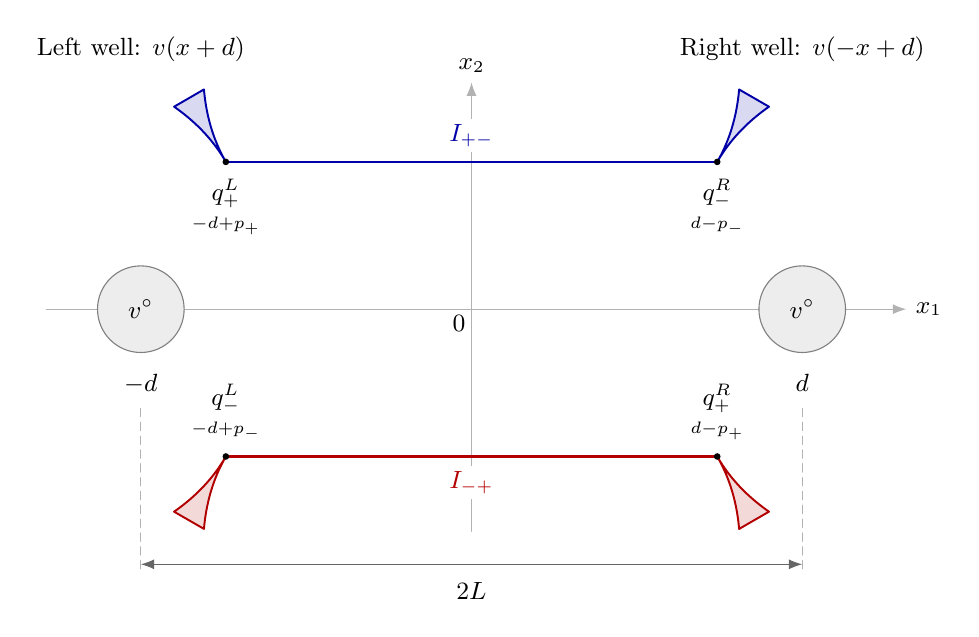
\begin{tikzpicture}[
  x=1.2cm,y=1.2cm,font=\small,
  line cap=round,line join=round,
  axis/.style={-{Latex[length=1.7mm]},black!30,thin},
  tiplabel/.style={align=center,inner sep=2pt}
]
  % Schematic dimensions.
  \def\figL{3.5}
  \def\figR{1.8}
  \pgfmathsetmacro{\figX}{\figL-\figR/2}
  \pgfmathsetmacro{\figY}{sqrt(3)*\figR/2}

  \coordinate (CL) at (-\figL,0);
  \coordinate (CR) at ( \figL,0);
  \coordinate (Lp) at (-\figX, \figY); % -d+p_+
  \coordinate (Lm) at (-\figX,-\figY); % -d+p_-
  \coordinate (Rm) at ( \figX, \figY); %  d-p_- (upper)
  \coordinate (Rp) at ( \figX,-\figY); %  d-p_+ (lower)

  % Axes and radial cores.
  \draw[axis] (-4.5,0) -- (4.6,0)
    node[right,text=black] {$x_1$};
  \draw[axis] (0,-2.35) -- (0,2.4)
    node[above,text=black] {$x_2$};
  \node[below left,inner sep=2pt] at (0,0) {$0$};

  \draw[black!50,fill=black!7] (CL) circle[radius=5.5mm]
    node[text=black] {$v^\circ$};
  \draw[black!50,fill=black!7] (CR) circle[radius=5.5mm]
    node[text=black] {$v^\circ$};
  \node[below=7mm] at (CL) {$-d$};
  \node[below=7mm] at (CR) {$d$};
  \node at (-\figL,2.75) {Left well: $v(x+d)$};
  \node at ( \figL,2.75) {Right well: $v(-x+d)$};

  % Quadratic cusps with local boundaries s = +/-0.30 t^2.
  % The right-hand cusps are obtained by inversion.
  \foreach \tipname/\cuspangle/\cuspcolor in {
    Lp/120/blue!65!black, Rm/60/blue!65!black,
    Lm/240/red!70!black, Rp/300/red!70!black}{
    \begin{scope}[shift={(\tipname)},rotate=\cuspangle]
      \path[draw=\cuspcolor,fill=\cuspcolor,fill opacity=0.15,
            line width=0.7pt]
        plot[domain=0:0.78,samples=25] (\x,{0.30*\x*\x})
        -- plot[domain=0.78:0,samples=25] (\x,{-0.30*\x*\x})
        -- cycle;
    \end{scope}
  }

  % The two dominant source pairings.
  \draw[blue!65!black,line width=1pt] (Lp) --
    node[above=3pt,fill=white,inner sep=2pt] {$I_{+-}$} (Rm);
  \draw[red!70!black,line width=1pt] (Lm) --
    node[below=3pt,fill=white,inner sep=2pt] {$I_{-+}$} (Rp);

  \foreach \tipname in {Lp,Lm,Rm,Rp}
    \fill (\tipname) circle[radius=1.2pt];

  \node[tiplabel,anchor=north,yshift=-4pt] at (Lp)
    {$q_+^L$\\[-1pt]$\scriptstyle -d+p_+$};
  \node[tiplabel,anchor=north,yshift=-4pt] at (Rm)
    {$q_-^R$\\[-1pt]$\scriptstyle d-p_-$};
  \node[tiplabel,anchor=south,yshift=4pt] at (Lm)
    {$q_-^L$\\[-1pt]$\scriptstyle -d+p_-$};
  \node[tiplabel,anchor=south,yshift=4pt] at (Rp)
    {$q_+^R$\\[-1pt]$\scriptstyle d-p_+$};

  % Separation of the well centers.
  \draw[black!30,densely dashed]
    (-\figL,-1.05) -- (-\figL,-2.8);
  \draw[black!30,densely dashed]
    ( \figL,-1.05) -- ( \figL,-2.8);
  \draw[{Latex[length=1.7mm]}-{Latex[length=1.7mm]},black!60]
    (-\figL,-2.7) --
    node[below=3pt,text=black] {$2L$} (\figL,-2.7);
\end{tikzpicture}
\caption{The two dominant cusp pairings in the inversion-symmetric
double well, with $d=(L,0)$ and $p_\pm=(R/2,\pm\sqrt{3}R/2)$.
Here $q_\pm^L(x)=q_\pm(x+d)$ and $q_\pm^R(x)=q_\pm(-x+d)$.
The upper pair joins $-d+p_+$ to $d-p_-$ and contributes $I_{+-}$;
the lower pair joins $-d+p_-$ to $d-p_+$ and contributes $I_{-+}$.
Thus opposite one-well labels correspond to cusps at the same physical
height. The colored segments denote source pairings in the hopping
integral. The geometry is schematic, with core sizes and cusp widths
enlarged for visibility.}
\label{fig:dominant-cusp-pairings}
\end{figure}

The choice of profile within each cusp is important. In the cusp
coordinates of \Cref{sec:construction}, its normal factor is
\[
 \exp\!\left[-\beta\left(\log\frac{t_*}{t}\right)^2\right],
 \qquad t>0,
\]
with fixed $\beta,t_*>0$ and smooth cutoffs away from the tip. This factor
vanishes to infinite order at $t=0$, so the sophons extend smoothly by zero.
The balance between this profile and the linear increase of the decay
action selects
\[
 t\asymp h\log(1/h).
\]
On this scale the transverse displacements contribute only
$\cO(h\log^2(1/h))=o(1)$ to the exponent and are therefore negligible.
Thus the fixed cusp geometry concentrates the leading interaction near
its tips as $h\to0$.

To evaluate that interaction, we first insert the radial ground-state
Ansatz into the hopping integral. In fact, outside the core the radial
ground state has the exact representation
\[
 \phi_h^\circ(x)=\Gamma_h K_h^{-E_h^\circ}(x),
 \qquad |x|>r_0,
 \qquad \Gamma_h>0,
\]
where $E_h^\circ$ is the scaled one-well energy and $K_h^\cE$ is the radial
amplitude factor of the Landau Hamiltonian resolvent, which has Gaussian
decay. Substituting its asymptotic expansion into the hopping integral,
we obtain an oscillatory integral whose exponent contains the two radial
decay actions, the action for propagation between the sophons (the
\emph{bridge action}), and the large magnetic phase. We then apply
steepest descent. The leading normal integrals take the form
\[
 \int_0^{t_0}t^2\chi_a(t)
 \exp\!\left[
 -\beta\left(\log\frac{t_*}{t}\right)^2
 -\frac{(\alpha-i\theta)t}{h}
 \right]\dd t,
 \qquad \alpha>0,
\]
where $\alpha$ and $\theta$ are the normal action and phase slopes, and the
factor $t^2$ comes from the cusp Jacobian. The logarithmic term produces
an $h$-dependent critical point near $t=0$. The complex saddle is described
by the principal branch of the Lambert-$W$ function. Holomorphic control
of the radial and resolvent expansions along the deformed contours gives
an error small relative to the positive envelope $\mathfrak a_h$.

Our use of the radial ground-state approximation to the exact one-well
ground state must be justified. On each sophon, we separate the source
into the incoming radial contribution and the scattered response generated
by the full perturbation $\eps(q_++q_-)$, including scattering involving
either cusp. The leading term contains two log-flat factors, one from each
sophon. Weighted resolvent estimates show that every term involving a
scattered response incurs at least one additional log-flat decay cost.
Such terms are smaller than the positive leading envelope by a factor
$e^{-c\log^2(1/h)}=o(h^N)$ for every fixed $N>0$, with $c>0$.
This separation allows the sophon amplitudes to remain fixed as $h=\lambda^{-1}\to0$.

As asserted in \Cref{eq:introestimrhol}, the two dominant contributions
are complex conjugates of one another and yield
\begin{align}\label{eq:cosine formula for rho}
 \rho_\lambda
 =-2|\mathscr C_*|\mathfrak a_{1/\lambda}
 \left[\cos\Theta(\lambda)
 +\cO\!\left((\log\lambda)^{-1}\right)\right],
 \qquad \mathscr C_*\ne0,
\end{align}
with the phase given by \Cref{eq:intro-phase}. The error in the spectral
reduction \Cref{eq:introestimgap}, divided by the positive envelope
$\mathfrak a_{1/\lambda}$, is $\mathcal O(e^{-c\lambda})$ for all
sufficiently large $\lambda$. This envelope measures the size of the
dominant contributions before their oscillatory cancellation and remains
positive even where $\rho_\lambda$ vanishes. At successive phase points
where the cosine is $+1$ and $-1$, the magnitude of $\rho_\lambda$ is
comparable to $\mathfrak a_{1/\lambda}$. The reduction error is therefore
too small to change the sign of $-2\rho_\lambda$, so the exact signed
splitting also alternates in sign. Continuity then yields infinitely many
hopping zeros and infinitely many exact eigenvalue crossings, although
the two sequences need not coincide.

\medskip\noindent\textbf{Organization of the paper.}
\Cref{sec:construction} constructs the fixed potential.
\Cref{sec:one-well-source} and~\Cref{sec:schur-reduction} control the
one-well source and carry out the parity Schur reductions.
\Cref{sec:exact-hopping} derives an exact formula for the hopping
coefficient (see also \cite[(2.29)]{FSW-absence}) and isolates the two
dominant contributions, which are evaluated in
\Cref{sec:active-integral}.
\Cref{sec:full-hopping-section} and~\Cref{sec:spectral-transfer}
establish the sign changes in the hopping coefficient and transfer them
to eigenvalue crossings in the exact spectrum of the magnetic double-well
Hamiltonian. The appendices contain auxiliary resolvent estimates\textcolor{blue}{,} the
complex steepest descent arguments and a formalization of the proof, up to classical results in the literature.

\begin{remark}
One can additionally impose reflection symmetry across the $x_2$-axis,
$v(-x_1,x_2)=v(x_1,x_2)$, resulting in four cusp components surrounding the
radial core instead of two. This symmetry is useful in multi-well
constructions; see \cite{FSW-PNAS}. Contributions from the additional cusp
components are negligible, as their actions are strictly larger than those
of the dominant contributions. Thus the same leading asymptotics hold.
\end{remark}

\begin{remark}
A similar asymptotic expansion in $L$ can be derived by the methods used
in the proof of \Cref{thm:main}. If we fix $\lambda$ instead of the
displacement $L$, the $L\to\infty$ asymptotic takes the form
\[
 \rho_L=-\cA_\lambda(L)\left[
 \cos\Theta_\lambda(L)+e^{-\frac34 b\lambda R^2}
 +O_\lambda\!\left(\frac{1}{\log L}\right)\right].
\]
Since $0<e^{-\frac34 b\lambda R^2}<1$, this yields infinitely many hopping
zeros provided $\cA_\lambda(L)>0$ and $\Theta_\lambda(L)$ is continuous and
unbounded. We shall return to these asymptotics and their spectral
consequences in \cite{FKSW-large-separation}.
\end{remark}

%\begin{remark}
%We previously found an example and subsequently used GPT-5.6 to help find
%the simpler example presented here. We take full responsibility for the
%contents of this paper.
%\end{remark}

\begin{remark}
The main difference from \cite{FSW-absence} is how the sophon contributions
are controlled. There, their $\lambda$-dependent sizes permit a perturbative
analysis; here, their fixed profiles are chosen so that the leading
interaction can be evaluated by contour deformation.
\end{remark}


\section*{AI statement}
The authors used a workflow combining ChatGPT Pro 5.5/5.6 and Claude Fable 5 during the development of this work. The authors first found an example independently and subsequently used AI models to help identify the simpler example presented here. This was achieved through a process of iterative prompting, refinement, and evaluation across multiple interactions rather than through a single model query thread. For example, we discarded several routes that were not promising and we refined the results of our main theorem multiple times. All mathematical statements and proofs were independently and rigorously verified by the authors, who take full responsibility for the contents of the paper.

\section*{Acknowledgements}
KB was partially supported by NSF under grant DMS-2434314. CF was supported in part by NSF grant DMS-1700180. JGS was partially supported by NSF, under Grants DMS-2245017,
DMS-2554957 and DMS-2434314. AH was partially supported by French National Research Agency (ANR), under grant ANR-24-ERCS-0010, and by Hi! PARIS and State funding managed by the ANR under the France 2030 program, ANR-23-IACL-0005. JS was supported in part by NSF grant DMS-2510207. MIW was supported in part by NSF grants DMS-1908657, DMS-1937254, DMS-2510769  and Simons Foundation Math + X Investigator Award \# 376319 (MIW). Part of this research was carried out during the 2023-24 academic year, when MIW was a Visiting Member in the School of Mathematics - Institute of Advanced Study, Princeton, supported by the Charles Simonyi Endowment, and a Visiting Fellow in the Department of Mathematics at Princeton University.

\section{Construction of the fixed potential}\label{sec:construction}

In this section we construct the potential
\begin{equation}\label{eq:voverview}
 v=v^\circ+\eps(q_++q_-).
\end{equation}
To begin, we will fix a radial core $v^\circ$ and control the exterior tail of its ground state.

We {will} then place two reflected one-sided cusps, $q_\pm$, at distance $R$ from the
core {as in \Cref{eq:cusplocation}} and fix their supports, log-flat profiles, and amplitudes.  These are treated as perturbations for our analysis, and their effects will be controlled. After the potential is
complete, a lower bound on the well separation is imposed by the action
certificate.

\subsection{Magnetic scaling and notation}\label{sec:framework}
Put $h=\lambda^{-1}$ and {introduce the semi-classically scaled Landau Hamiltonian}:
\begin{equation}\label{eq:Dh}
 H_h^L:=\left(hP-\frac b2x^\perp\right)^2.
\end{equation}
For a one-well potential $u$, write
\[
 H_h^{\rm atom}(u)=H_h^L+u.
\]

\subsection{The radial reference well}\label{sec:radial-one-well}
Fix $r_0>0$, and take the explicit radial core $v^\circ$ by
\begin{equation}\label{eq:explicit-core}
 v^\circ(x):=
 \begin{cases}
 -\exp\!\left(-\dfrac{|x|^2}{r_0^2-|x|^2}\right),&|x|<r_0,\\[1ex]
 0,&|x|\ge r_0.
 \end{cases}
\end{equation}
Then $v^\circ\in C_c^\infty(\R^2;[-1,0])$ and has the unique global minimum $v^\circ(0)=-1$. 
Additionally,
 $\nabla^2v^\circ(0)=\omega^2 I$ and $\omega^2=2/r_0^2$.
Denote the normalized ground-state pair of $H_h^{\rm atom}(v^\circ)$ by $(E_h^\circ,\phi_h^\circ)$.

\subsubsection{Radial spectral data}
Next compute the relevant properties of the base well, beginning with its energy and gap.
\begin{lemma}[Radial one-well energy and gap]\label{lem:radial-spectral}
Let
\begin{equation}\label{eq:oscillator-operator}
 \mathcal H_{\rm osc}
 :=\left(-i\nabla_y-\frac b2y^\perp\right)^2
 +\frac{\omega^2}{2}|y|^2,
\end{equation}
and let $(\mu_0,\psi_0)$ be its normalized positive ground pair.  There are
$h_0,c_{\rm gap}>0$ such that, for $0<h<h_0$,
\begin{equation}\label{eq:base-energy}
 E_h^\circ=-1+\mu_0h+\cO(h^{3/2}),
\end{equation}
and
\begin{equation}\label{eq:base-gap}
 \dist\!\left(E_h^\circ,\sigma(H_h^{\rm atom}(v^\circ))\setminus\{E_h^\circ\}\right)
 \ge c_{\rm gap}h.
\end{equation}
The ground state is simple, radial, and can be chosen as a strictly positive
function of $r$. Moreover, for
\begin{equation}\label{eq:rescaled-radial-ground-state}
 \psi_h(y):=h^{1/2}\phi_h^\circ(h^{1/2}y),
\end{equation}
one has $\psi_h\to\psi_0$ strongly in $L^2_{\rm loc}(\R^2)$. \end{lemma}

\begin{proof}
{This follows directly from \cite{HK24}.}
Noting the scaling relation
$H_h^{\rm atom}(v^\circ)=b^2\mathcal L_{h/b}^{\rm sw}(v^\circ/b^2)$ in the notation of
\cite[Theorem~1.1, Proposition~2.1]{HK24}, the energy expansion and the
order-$h$ gap follow from those results.  Ground-state simplicity, radiality,
strict positivity, and strong local convergence of the rescaled ground state follow from the rotational symmetry and the ground-state
characterization in \cite[Proposition~2.1]{HK24}.

\begin{formalisationaddition}{L2.1}
We keep the radial harmonic approximation as an explicitly identified spectral input, and separate its normalization from the calculations needed below. All scalar products are conjugate-linear in the first argument.

\begin{lemma}[Expansion of the fixed radial core]\label{sublemma:L2-1-core-taylor}
The potential in \eqref{eq:explicit-core} has its unique minimum $-1$ at $0$, and
\[
 v^\circ(x)=-1+\frac{|x|^2}{r_0^2}+O(|x|^4),\qquad
 D^2v^\circ(0)=\omega^2 I,\quad \omega^2=2/r_0^2.
\]
\end{lemma}
\begin{proof}
For $q=|x|^2<r_0^2$, write
$q/(r_0^2-q)=q/r_0^2+O(q^2)$ and use $e^{-z}=1-z+O(z^2)$.
The exponent is zero only at $q=0$ and strictly negative otherwise; outside the ball the potential is zero. The quadratic Taylor coefficient gives the Hessian. At the boundary, writing $r_0^2-q=s>0$ gives $v^\circ=-e\exp(-r_0^2/s)$; every derivative tends to zero as $s\downarrow0$. Thus extension by zero is smooth.
\end{proof}

\begin{lemma}[Unitary rescaling and limiting oscillator]\label{sublemma:L2-1-rescale}
The map $(V_hf)(y)=h^{1/2}f(\sqrt h\,y)$ is unitary on $L^2(\R^2)$. On compact sets,
\[
 V_h\frac{\Ho+1}{h}V_h^{-1}
 =\left(-i\nabla_y-\frac b2y^\perp\right)^2+
   \frac{v^\circ(\sqrt h\,y)+1}{h}
 =H_{\rm osc}+O(h|y|^4).
\]
\end{lemma}
\begin{proof}
The substitution $x=\sqrt h\,y$ has Jacobian $h$, which cancels the squared prefactor. Moreover
$V_h(hP_x)V_h^{-1}=\sqrt h P_y$ and
$V_h x V_h^{-1}=\sqrt h y$. Squaring the covariant momentum therefore produces exactly the factor $h$. Apply the preceding Taylor expansion; for every fixed compact set the error and any prescribed finite number of its derivatives are uniformly controlled.
\end{proof}

\begin{lemma}[Oscillator ground state and positive limiting gap]\label{sublemma:L2-1-oscillator}
Put $\nu=(b^2/4+\omega^2/2)^{1/2}$. The normalized oscillator ground state and its energy are
\[
 \psi_0(y)=\sqrt{\nu/\pi}\,e^{-\nu|y|^2/2},\qquad \mu_0=2\nu.
\]
The ground state is simple and the next oscillator energy is $\mu_0+(2\nu-b)$, where $2\nu-b>0$.
\end{lemma}
\begin{proof}
Expanding the square gives $H_{\rm osc}=-\Delta+\nu^2|y|^2-bL_z$, where $L_z=-i(y_1\partial_2-y_2\partial_1)$. The displayed Gaussian has $L_z\psi_0=0$ and
$-\Delta\psi_0=(2\nu-\nu^2|y|^2)\psi_0$; its squared integral is $(\nu/\pi)(\pi/\nu)=1$.
The two-dimensional isotropic oscillator, decomposed into angular modes $m\in\mathbb Z$ and radial indices $n\ge0$, has energies
$2\nu(2n+|m|+1)-bm$.
Subtracting $2\nu$ gives $4\nu n+2\nu|m|-bm\ge(2\nu-b)|m|+4\nu n$.
Since $\omega>0$, $\nu>b/2$. The smallest positive difference is attained at $(n,m)=(0,1)$ and equals $2\nu-b$. This also proves simplicity of the ground state. The standard oscillator mode decomposition is the spectral input to this last computation.
\end{proof}

\interface{The radial one-well harmonic-approximation theorem used in the original proof is [8, Theorem 1.1 and Proposition 2.1]: a smooth radial compactly supported well with a unique nondegenerate minimum has, after the above rescaling, convergence of the first fixed low eigenvalues to those of the oscillator, the ground-energy remainder $O(h^{3/2})$, a simple angular-momentum-zero positive ground state for small $h$, and convergence of its normalized rescaled eigenfunction locally in $L^2$. This is an external PDE/spectral theorem, not a finite calculation being hidden in a new sublemma. Its application requires precisely the hypotheses checked above. In the normalization of [8], use $\Ho=b^2L^{\rm sw}_{h/b}(v^\circ/b^2)$; both sides expand to the same differential expression.}

\begin{lemma}[Transfer of a separated oscillator pair]\label{sublemma:L2-1-gap-transfer}
If the first two rescaled eigenvalues converge to $\mu_0$ and $\mu_1>\mu_0$, then for small $h$ their unscaled difference is at least $\frac12(\mu_1-\mu_0)h$.
\end{lemma}
\begin{proof}
Choose $h_0$ so both rescaled errors have modulus at most $(\mu_1-\mu_0)/4$. Subtract the two inequalities and multiply by $h>0$. Adding the same shift $-1$ to both eigenvalues does not change their difference.
\end{proof}
\finish Apply this transfer with $\mu_1-\mu_0=2\nu-b$, and the stated radial harmonic approximation. It gives \eqref{eq:base-energy}--\eqref{eq:rescaled-radial-ground-state}, including the phase choice $\psi_h\to\psi_0$ and positivity of $\phi_h^\circ$. The constant $c_{\rm gap}$ may be any fixed positive number smaller than $(2\nu-b)/2$.
\end{formalisationaddition}

\end{proof}

In particular, after decreasing $h_0$ if necessary,
\begin{equation}\label{eq:radial-energy-window}
 \frac12<-E_h^\circ<\frac32.
\end{equation}
Thus the exterior energy parameter $\cE_h^\circ=-E_h^\circ$ remains in one
fixed compact subinterval of $(0,\infty)$, as required by the uniform
Landau-kernel estimates below. 

\subsection{Exact exterior tail and the bridge action}\label{sec:radial-exterior-tail}
Next we compute the exterior tail of the core well and its corresponding bridge action. Note that outside $\supp v^\circ$, the radial ground state solves the free Landau
equation
\[
 (H_h^L-E_h^\circ)\phi_h^\circ=0.
\]
Since $\cE_h^\circ=-E_h^\circ>0$ for small $h$, its decaying exterior branch is governed by the free Landau resolvent $(H_h^L+\cE)^{-1}$.  We first identify the exact resolvent representation and the exponential rate that it determines.

\subsubsection{Landau resolvent and the bridge action}
For $\cE>0$, the semigroup representation gives
\[
 (H_h^L+\cE)^{-1}
 =\int_0^\infty e^{-t\cE}e^{-tH_h^L}\,\dd t.
\]
In the symmetric gauge, the exact Landau heat kernel is
\[
 e^{-tH_h^L}(x,y)
 =\frac{b}{4\pi h\sinh(bht)}
 e^{-\frac{ib}{2h}x\wedgep y}
 \exp\!\left[-\frac{b}{4h}\coth(bht)|x-y|^2\right].
\]

Consequently, the Landau resolvent $(H_h^L+\cE)^{-1}$ has the symmetric-gauge kernel
\begin{equation}\label{eq:landau-kernel-master}
 (H_h^L+\cE)^{-1}(x,y)
 =e^{-\frac{ib}{2h}x\wedgep y}K_h^\cE(x-y),
\end{equation}
where $K_h^\cE$ is radial and real-valued.   After the change of variables $\tau=ht$, its radial part is
\begin{equation}\label{eq:K-integral}
 K_h^{\cE}(r)
 =\frac{b}{4\pi h^2}
 \int_0^\infty
 \frac{1}{\sinh(b\tau)}
 \exp\!\left[-\frac1h\left(
 \cE\tau+\frac b4\coth(b\tau)r^2
 \right)\right]\dd\tau,
 \qquad r>0.
\end{equation}
Set
\[
 \mathcal H(\tau;r,\cE)
 :=\cE\tau+\frac b4\coth(b\tau)r^2.
\]
Thus \Cref{eq:K-integral} is a one-dimensional Laplace integral with phase $\mathcal H$.  Its exponential rate is therefore the minimum of this phase in the proper-time variable.  We define the bridge action by
\begin{equation}\label{eq:J}
 \cJ_\cE(r)
 :=\inf_{\tau>0}\mathcal H(\tau;r,\cE)
 =\inf_{\tau>0}\left(\cE\tau+\frac b4\coth(b\tau)r^2\right).
\end{equation}
The point of this representation is that the same function $\cJ_\cE$ will govern both the Landau resolvent decay and the exterior radial tail.

\begin{proposition} \label{prop:Jminimizer}
For $r>0$ and $\cE>0$, the infimum in \Cref{eq:J} is attained at a unique point $\tau_*(r,\cE)>0$, which satisfies
\begin{equation}\label{eq:radial-tau-star}
 \sinh(b\tau_*(r,\cE))=\frac{br}{2\sqrt\cE}.
\end{equation}
Consequently,
\begin{align}
 \cJ_\cE(r)
 &=\frac{\cE}{b}\operatorname{arsinh}\!\left(\frac{br}{2\sqrt\cE}\right)
 +\frac b4r^2\sqrt{1+\frac{4\cE}{b^2r^2}},\label{eq:J-explicit}\\
 \partial_r\cJ_\cE(r)
 &=\frac12\sqrt{b^2r^2+4\cE}.
 \label{eq:radial-J-prime}
\end{align}
In particular,
\begin{equation}\label{eq:J-eikonal}
 \bigl(\partial_r\cJ_\cE(r)\bigr)^2
 =\cE+\frac{b^2r^2}{4},
 \qquad
 \cJ_\cE(r)
 =\int_0^r\sqrt{\cE+\frac{b^2s^2}{4}}\,\dd s.
\end{equation}
\end{proposition}
\begin{proof}
Differentiating the phase gives
\[
 \partial_\tau\mathcal H
 =\cE-\frac{b^2r^2}{4}\operatorname{csch}^2(b\tau),
\]
which strictly increases from $-\infty$ to $\cE$ on $(0,\infty)$.  Hence it
has a unique zero, and solving the critical-point equation gives
\Cref{eq:radial-tau-star}.  Moreover,
\[
 \partial_\tau^2\mathcal H(\tau_*)
 =\frac{b^3r^2}{2}\operatorname{csch}^2(b\tau_*)
  \coth(b\tau_*)>0.
\]
Put $s=br/(2\sqrt\cE)$.  At the critical point,
$b\tau_*=\operatorname{arsinh}s$ and
$\coth(b\tau_*)=\sqrt{1+s^2}/s$.  Substitution in
\Cref{eq:J} yields \Cref{eq:J-explicit}.  Finally, the critical point is
nondegenerate, so differentiation of the minimized action with respect to
$r$ gives
\[
 \partial_r\cJ_\cE(r)
 =\partial_r\mathcal H(\tau_*;r,\cE)
 =\frac b2r\coth(b\tau_*)
 =\frac12\sqrt{b^2r^2+4\cE},
\]
which is \Cref{eq:radial-J-prime}.  Squaring gives the eikonal identity in
\Cref{eq:J-eikonal}. Since $\cJ_\cE$ extends continuously to $r=0$ with $\cJ_\cE(0)=0$, integration yields the second formula there.

\begin{formalisationaddition}{P2.2}
Throughout this proof $b,r,E>0$ are fixed and $H(\tau)=E\tau+(br^2/4)\coth(b\tau)$.

\begin{lemma}[Derivatives and unique critical point]\label{sublemma:P2-2-critical}
For $\tau>0$,
\[
 H_\tau=E-\frac{b^2r^2}{4\sinh^2(b\tau)},\qquad
 H_{\tau\tau}=\frac{b^3r^2}{2}\frac{\cosh(b\tau)}{\sinh^3(b\tau)}>0.
\]
The unique minimum is attained at
$\tau_*=b^{-1}\operatorname{arsinh}(br/(2\sqrt E))$.
\end{lemma}
\begin{proof}
Differentiate $\coth x$ using $(\coth x)'=-\sinh^{-2}x$, and differentiate once more. As $\tau\downarrow0$, $H(\tau)\sim r^2/(4\tau)$ and $H_\tau\to-\infty$. As $\tau\to\infty$, $H(\tau)\to\infty$ and $H_\tau\to E>0$. Strict monotonicity of $H_\tau$ therefore gives exactly one zero and a global minimum. Solving $H_\tau=0$ gives $\sinh(b\tau_*)=br/(2\sqrt E)$, which is \eqref{eq:radial-tau-star}.
\end{proof}

\begin{lemma}[Value of the minimum]\label{sublemma:P2-2-action-value}
One has
\[
 \cJ_E(r)=\frac r4\sqrt{b^2r^2+4E}
       +\frac Eb\operatorname{arsinh}\frac{br}{2\sqrt E}.
\]
\end{lemma}
\begin{proof}
Put $z=br/(2\sqrt E)>0$. Then $\cosh(b\tau_*)=\sqrt{1+z^2}$ and $\coth(b\tau_*)=\sqrt{1+z^2}/z$. Consequently $(br^2/4)\coth(b\tau_*)=(r/4)\sqrt{b^2r^2+4E}$, while $E\tau_*=(E/b)\operatorname{arsinh}z$. Add these terms. This proves \eqref{eq:J-explicit}; replacing $\operatorname{arsinh}z$ by $\log(z+\sqrt{1+z^2})$ gives the equivalent logarithmic form.
\end{proof}

\begin{lemma}[Radial derivative and integral representation]\label{sublemma:P2-2-action-derivatives}
For $r>0$,
\[
 \cJ_E'(r)=\frac12\sqrt{b^2r^2+4E},\quad
 \cJ_E''(r)=\frac{b^2r}{2\sqrt{b^2r^2+4E}}>0,\quad
 \partial_EJ_E(r)=\tau_*(r,E).
\]
Furthermore $\cJ_E(0)=0$ by continuous extension and
$\cJ_E(r)=\int_0^r\sqrt{E+b^2s^2/4}\,\mathrm ds$.
\end{lemma}
\begin{proof}
The explicit formula for $\tau_*$ is smooth. The chain rule applied to $H(\tau_*(r,E);r,E)$ has no critical-point derivative contribution, since $H_\tau(\tau_*)=0$. Thus $\cJ_E'=(br/2)\coth(b\tau_*)$, which simplifies to the displayed square root, and $\partial_EJ_E=\tau_*$. Differentiate the square root to obtain $\cJ_E''$. Both terms in the preceding explicit value tend to zero as $r\downarrow0$; the fundamental theorem of calculus then gives the integral representation. Squaring the positive derivative gives $(\cJ_E')^2=E+b^2r^2/4$.
\end{proof}

\begin{lemma}[Useful large-radius and squared-radius bounds]\label{sublemma:P2-2-growth}
For $s>0$,
$\frac{\mathrm d}{\mathrm ds}\cJ_E(\sqrt s)=\frac14\sqrt{b^2+4E/s}\ge b/4$.
On every compact positive energy interval, $\cJ_E(r)=br^2/4+O(1+\log r)$ as $r\to\infty$.
\end{lemma}
\begin{proof}
Apply the chain rule to the previous derivative. For $r\ge1$ rationalization gives
\[
0\le \cJ_E'(r)-br/2
=\frac{2E}{\sqrt{b^2r^2+4E}+br}\le \frac{E}{br}.
\]
Integrate between $1$ and $r$; the integral on $[0,1]$ is uniformly bounded for the stated energies.
\end{proof}
\finish These sublemmas prove all the identities and uniqueness assertions in the proposition, as well as the growth estimate subsequently used in \eqref{eq:J-large-r}.
\end{formalisationaddition}

\end{proof}

As a useful consequence of the explicit formula, uniformly for $\cE$ in a compact subset of $(0,\infty)$, the large-$r$ expansions give that the explicit action satisfies
\begin{equation}\label{eq:J-large-r}
 \cJ_\cE(r)=\frac b4r^2+\cO(\log(2+r)),\qquad r\to\infty.
\end{equation}

\subsubsection{Landau kernel asymptotics}
We next apply Laplace's method to \Cref{eq:K-integral}.  This gives the complete differentiated expansion of the Landau kernel with exponential rate $\cJ_\cE$.
\begin{proposition}[Differentiated radial Laplace expansion]\label{prop:K-Laplace}
Fix compact intervals $I_r\Subset(0,\infty)$ and $I_\cE\Subset(0,\infty)$.  For every $N,k$ there are smooth functions $k_j(r,\cE)$, $0\le j<N$, such that, uniformly for $(r,\cE)\in I_r\times I_\cE$,
\begin{equation}\label{eq:K-expansion}
 K_h^\cE(r)
 =h^{-3/2}e^{-\cJ_\cE(r)/h}
 \left(\sum_{j=0}^{N-1}h^jk_j(r,\cE)+h^NR_{N,h}(r,\cE)\right),
\end{equation}
with
\begin{equation}\label{eq:K-remainder}
 \sup_{0\le \ell+m\le k}
 \abs{\partial_r^\ell\partial_\cE^mR_{N,h}(r,\cE)}\le C_{N,k}.
\end{equation}
The leading coefficient is strictly positive:
\begin{equation}\label{eq:k0}
 k_0(r,\cE)
 =\frac{b}{4\pi\sinh(b\tau_*)}
 \left(\frac{2\pi}{\partial_\tau^2\mathcal{H}(\tau_*;r,\cE)}\right)^{1/2}>0,
\end{equation}
where $\tau_*=\tau_*(r,\cE)$ is the minimizer from \Cref{prop:Jminimizer}.  The asymptotic expansion remains valid after taking any fixed spatial derivative provided one uses the rescaled derivative $(h\partial_{x})^{\alpha} = h^{|\alpha|}\partial_{x}^{\alpha}.$
\end{proposition}

\begin{proof}
For $(r,\cE)$ in the stated compact sets, the two ends of the integral {of \Cref{eq:K-integral}} are uniformly negligible because
\[
 \mathcal H(\tau;r,\cE)\sim \frac{r^2}{4\tau}
 \quad (\tau\downarrow0),
 \qquad
 \mathcal H(\tau;r,\cE)\sim \cE\tau+\frac{br^2}{4}
 \quad (\tau\to\infty).
\]
After restricting to a fixed compact interval in $\tau$, split \Cref{eq:K-integral} into a fixed neighborhood of $\tau_*$ and its complement.  On the complement, $\mathcal H$ exceeds its minimum by a fixed positive amount.  Since $e^{-\delta/h}$ decays faster than every power of $h$, the asymptotic expansion comes only from a neighborhood of $\tau_*$.  In that neighborhood use the Morse coordinate
\[
    y^2=2\bigl(H(\tau;r,E)-H(\tau_*;r,E)\bigr),
    \qquad {\operatorname{sgn} y=\operatorname{sgn}(\tau-\tau_*)}.
\]
{ Since the critical point is uniformly nondegenerate, this defines a
smooth change of variables $\tau=T(y;r,E)$, uniformly for
$(r,E)\in I_r\times I_E$, with
\[
    T(0;r,E)=\tau_*(r,E),
    \qquad
    \partial_y T(0;r,E)
    =\bigl(\partial_\tau^2H(\tau_*;r,E)\bigr)^{-1/2}.
\]
Thus the contribution from this neighborhood is
\[
 \frac{b}{4\pi h^2}e^{-J_E(r)/h}
 \int
 \frac{\partial_yT(y;r,E)}
      {\sinh(bT(y;r,E))}
 e^{-y^2/(2h)}\,dy.
\]
Taylor expand the smooth amplitude inside the integral at  $y=0$.  The odd Taylor terms integrate to zero, up to exponentially
small errors from the truncated Gaussian tails, while
\[
 \int_{\mathbb R} y^{2j}e^{-y^2/(2h)}\,dy
 = \sqrt{2\pi h}\,\frac{(2j)!}{2^j j!}\,h^j.
\]
It follows that the integral has a complete expansion in integer powers
of $h$.  Together with the prefactor $h^{-2}$, the Gaussian factor
$\sqrt h$ gives the overall power $h^{-3/2}$ in \Cref{eq:K-expansion}.  The
leading coefficient is
\[
 k_0(r,E)
 =\frac{b}{4\pi\sinh(b\tau_*)}
   \left(
      \frac{2\pi}
           {\partial_\tau^2H(\tau_*;r,E)}
   \right)^{1/2}>0,
\]
This} gives \Cref{eq:K-expansion}--\Cref{eq:k0}.  Uniform differentiated bounds follow because all critical-point derivatives are uniform on compact sets.  Spatial differentiation either differentiates a smooth coefficient or produces $h^{-1}\partial_r\cJ$; multiplying by the corresponding power of $h$ gives the final assertion.

\begin{formalisationaddition}{P2.3}
Write $p=(r,E)$, $J(p)=\cJ_E(r)$,
$a(\tau)=b/(4\pi\sinh(b\tau))$, and
$H(\tau;p)=E\tau+(br^2/4)\coth(b\tau)$. In this proof $E>0$ denotes the
positive resolvent parameter, not the negative eigenvalue. Choose compact
rectangles $P\subset\operatorname{int}P_1\subset(0,\infty)^2$, where
$P=I_r\times I_\cE$. All differentiations below are carried out on $P_1$
before restriction to $P$. Taylor remainder arguments use $N\ge1$;
the order-zero bounded expansion follows immediately from the case $N=1$.

\interface{The inputs used for the scalar analysis are the parameter-dependent
inverse-function theorem, differentiation under an integral with an integrable
majorant, and the real Gaussian integral. The Landau heat-kernel representation
is the already stated identity \Cref{eq:K-integral}. No asymptotic expansion
of this integral is taken as an additional input.}

\begin{lemma}[A compact critical graph with positive Hessian]\label{sublemma:P2-3-critical-compact}
There are $0<a_*<b_*<\infty$ and $m_*>0$ such that, on $P_1$,
$a_*\le\tau_*(p)\le b_*$ and
$H_{\tau\tau}(\tau_*(p);p)\ge m_*$. Every fixed derivative of
$\tau_*$ and $J$ is bounded there.
\end{lemma}
\begin{proof}
The explicit formula in \Cref{prop:Jminimizer} is
$\tau_*=b^{-1}\operatorname{arsinh}(br/(2\sqrt E))$.
It is positive and smooth for $r,E>0$. Its minimum and maximum on the
compact rectangle give $a_*,b_*$. The formula
$H_{\tau\tau}=b^3r^2\cosh(b\tau)/(2\sinh^3(b\tau))$ is positive on
this graph, so its minimum is positive as well. Smoothness of the explicit
formulas on a neighborhood of $P_1$ bounds all fixed derivatives.
\end{proof}

\begin{lemma}[Endpoint majorants, including differentiated amplitudes]\label{sublemma:P2-3-endpoint-majorants}
For any fixed parameter derivative order $m$, sufficiently small $\tau_-$
and sufficiently large $\tau_+$ can be chosen so that the normalized
endpoint integrands and their derivatives have integrable bounds of the form
\[
 C h^{-M}(1+\tau^M+\tau^{-M})a(\tau)
 e^{-\delta/h}
 \begin{cases}e^{-c/(h\tau)},&0<\tau<\tau_-,\\
 e^{-c\tau/h},&\tau>\tau_+.
 \end{cases}
\]
Here normalization means multiplication by $e^{J(p)/h}$, and all constants
are uniform in $p\in P_1$ and $0<h<1$.
\end{lemma}
\begin{proof}
If $r\ge r_->0$ and $E\ge E_->0$, then
$\coth(b\tau)\ge1/(b\tau)$ implies $H\ge r_-^2/(4\tau)$,
and $H\ge E_-\tau$. Also $J\le \cJ_+$ on $P_1$.
Decrease $\tau_-$ so $r_-^2/(8\tau)\ge \cJ_++\delta$ on that tail;
then $H-J\ge\delta+r_-^2/(8\tau)$. Increase $\tau_+$ so
$E_-\tau/2\ge \cJ_++\delta$, giving $H-J\ge\delta+E_-\tau/2$.
Parameter differentiation of $e^{-(H-J)/h}$ gives finite sums of products
of derivatives of $H-J$, with at most a fixed power of $h^{-1}$.
Those derivatives grow at most polynomially in $\tau,\tau^{-1}$.
The amplitude is $O(\tau^{-1})$ at zero and $O(e^{-b\tau})$ at infinity.
For integrability near zero use $u=1/\tau$; near infinity use the displayed
linear exponential. Reserving half of either endpoint exponential absorbs
all the fixed polynomial factors. This argument also justifies the claimed
bounds for any specified finite number of derivatives.
\end{proof}

\begin{lemma}[A uniform gap away from the critical graph]\label{sublemma:P2-3-offgraph-gap}
For any sufficiently small fixed $\epsilon>0$, the minimum of $H-J$ on
\[
 \{(\tau,p):\tau_-\le\tau\le\tau_+,\ p\in P_1,
                  |\tau-\tau_*(p)|\ge\epsilon\}
\]
is strictly positive.
\end{lemma}
\begin{proof}
This set is closed in a compact rectangle and hence compact. The function
$H-J$ is continuous, nonnegative, and vanishes exactly when
$\tau=\tau_*(p)$, by \Cref{prop:Jminimizer}. The set excludes all such
points. Its attained minimum is consequently positive. If the set is empty,
any positive gap works. This is a statement uniform in parameters, not just
a collection of pointwise strict inequalities.
\end{proof}

\begin{lemma}[Uniformly negligible noncritical heat times]\label{sublemma:P2-3-tails}
For a smooth localization equal to one near the critical graph, the
complementary integral $I_{\rm far}(p,h)$ satisfies, for every fixed
multi-index $\gamma$,
\[
 |\partial_p^\gamma(e^{J(p)/h}I_{\rm far}(p,h))|
       \le C_\gamma h^{-M_\gamma}e^{-\delta/h}.
\]
In particular $h^{-N-1/2}e^{J/h}I_{\rm far}$ and each fixed parameter
derivative are bounded, for every fixed $N$.
\end{lemma}
\begin{proof}
Use \ref{sublemma:P2-3-endpoint-majorants} at the endpoints and
\ref{sublemma:P2-3-offgraph-gap} on the compact middle interval.
Derivatives of the localization are supported in the same gapped middle
region and are bounded. Differentiation under the integral follows from
the endpoint majorants. Finally, for $q\ge0$ and $\delta>0$,
$h^{-q}e^{-\delta/h}\to0$: put $x=1/h$ and note
$q\log x-\delta x\to-\infty$. This also absorbs the factor $h^{-N-1/2}$.
\end{proof}

\begin{lemma}[Exact factorization of the phase at its minimum]\label{sublemma:P2-3-phase-factor}
Set $d=\tau-\tau_*(p)$ and
\[
 B(\tau,p)=2\int_0^1(1-s)
 H_{\tau\tau}(\tau_*(p)+sd;p)\,\mathrm ds.
\]
Then $H(\tau;p)-J(p)=d^2B(\tau,p)/2$ and
$B(\tau_*(p),p)=H_{\tau\tau}(\tau_*(p);p)$.
On a fixed neighborhood of the graph, $B\ge m_*/2$.
\end{lemma}
\begin{proof}
Apply the fundamental theorem of calculus twice to
$s\mapsto H(\tau_*+sd;p)$; the constant term is $J$ and the first
order term is zero. At $d=0$, $2\int_0^1(1-s)\,\mathrm ds=1$.
Uniform continuity of $H_{\tau\tau}$ near the compact graph and
\ref{sublemma:P2-3-critical-compact} give the last bound after the
neighborhood is decreased.
\end{proof}

\begin{lemma}[Uniform real Morse coordinate and coefficient formula]\label{sublemma:P2-3-morse}
The coordinate $y=d\sqrt{B(\tau,p)}$ has a smooth increasing inverse
$\tau=T(y;p)$ for $|y|<2\rho$, with one $\rho>0$ for all $p\in P_1$
after a harmless restriction of the parameter neighborhood. It satisfies
\[
 H(T(y;p);p)=J(p)+y^2/2,\qquad
 T_y(0;p)=H_{\tau\tau}(\tau_*(p);p)^{-1/2}.
\]
Its fixed derivatives are uniformly bounded on smaller neighborhoods.
\end{lemma}
\begin{proof}
The preceding factorization gives the phase identity. At $d=0$,
$\partial_\tau y=\sqrt{H_{\tau\tau}(\tau_*;p)}>0$.
The inverse-function theorem gives local inverses; uniform continuity
makes this derivative bounded below on a common tube around the graph.
Strict increase in $\tau$ gives uniqueness, so overlapping local inverses
agree. Compactness gives a common $y$ interval. Differentiating
$y(T(y;p),p)=y$ gives the displayed derivative and, iteratively, all fixed
derivative bounds; the denominator $\partial_\tau y$ stays bounded away
from zero.
\end{proof}

\begin{lemma}[A fixed integration domain after localization]\label{sublemma:P2-3-fixed-amplitude}
Choose an even smooth cutoff $\chi(y)$, equal to one for $|y|\le\rho/2$
and supported in $(-\rho,\rho)$. The function
\[
 A(y,p)=\chi(y)a(T(y;p))T_y(y;p)
\]
extended by zero is smooth on $\R\times P_1$, with bounded fixed mixed
derivatives. The localized heat-time integral is exactly
$e^{-J/h}\int_\R A(y,p)e^{-y^2/(2h)}\,\mathrm dy$.
\end{lemma}
\begin{proof}
The support of $\chi$ is strictly inside the domain of $T$, so extension
by zero creates no boundary derivative. Apply the increasing change of
variables from \ref{sublemma:P2-3-morse}. The complementary heat-time
localization vanishes near the critical graph and is covered by
\ref{sublemma:P2-3-tails}. Most importantly, the new integration domain
and the cutoff do not depend on $p$; no moving-boundary term appears in
subsequent parameter differentiations.
\end{proof}

\begin{lemma}[Gaussian recurrence and parity]\label{sublemma:P2-3-moment-recurrence}
For $h>0$, put $M_j(h)=\int_\R y^je^{-y^2/(2h)}\,\mathrm dy$.
All these integrals are absolutely convergent,
$M_{2j+1}=0$, $M_0=\sqrt{2\pi h}$, and
$M_{2j}=(2j-1)hM_{2j-2}$ for $j\ge1$.
\end{lemma}
\begin{proof}
Polynomial factors are dominated by a smaller Gaussian at infinity.
Reflection $y\mapsto-y$ gives the odd identity. The substitution
$y=\sqrt h\,x$ reduces $M_0$ to the real Gaussian integral.
For $j\ge1$, integrate the derivative of
$y^{2j-1}e^{-y^2/(2h)}$ on $[-R,R]$. Its boundary values tend to zero.
The identity
$0=(2j-1)M_{2j-2}-h^{-1}M_{2j}$ gives the recurrence.
\end{proof}

\begin{lemma}[Gaussian moments and the integrated Taylor remainder]\label{sublemma:P2-3-gaussian}
For $j\ge0$,
\[
 M_{2j}(h)=\sqrt{2\pi h}\frac{(2j)!}{2^jj!}h^j.
\]
If $A$ has bounded $2N$th $y$ derivative, its Taylor remainder after degree
$2N-1$ integrates against the Gaussian with absolute value at most
$C_N h^{N+1/2}$. The same assertion holds for a fixed parameter derivative
when the corresponding mixed derivative of $A$ is bounded.
\end{lemma}
\begin{proof}
Induct using \ref{sublemma:P2-3-moment-recurrence} and
$(2j)!/(2^jj!)=(2j-1)(2j-2)!/(2^{j-1}(j-1)!)$.
Taylor's integral remainder on the real line is
\[
 R(y,p)=\frac{y^{2N}}{(2N-1)!}\int_0^1(1-s)^{2N-1}
                   \partial_y^{2N}A(sy,p)\,\mathrm ds.
\]
Thus $|R|\le C|y|^{2N}$. The moment formula proves the bound.
Apply this same identity to $\partial_p^\gamma A$ for differentiated
remainders. The compactly supported amplitude in
\ref{sublemma:P2-3-fixed-amplitude} has all the required global bounds.
\end{proof}

\begin{lemma}[Coefficients and the power of the semiclassical prefactor]\label{sublemma:P2-3-coefficients}
The expansion coefficients are
\[
 k_j(p)=\frac{\sqrt{2\pi}}{2^jj!}\partial_y^{2j}A(0,p).
\]
The local kernel equals
$h^{-3/2}e^{-J/h}(\sum_{j<N}h^jk_j+O(h^N))$.
For $j=0$ this gives exactly the positive coefficient in \Cref{eq:k0}.
\end{lemma}
\begin{proof}
The Taylor coefficient of $y^{2j}$ is
$\partial_y^{2j}A(0,p)/(2j)!$. Multiply by the moment in the preceding
sublemma; the factorials cancel to give the displayed $k_j$.
Odd powers integrate to zero. The heat-kernel prefactor is $h^{-2}$,
and the Gaussian contributes $h^{1/2}$, so $h^{-2}h^{1/2}=h^{-3/2}$.
At $y=0$, $\chi=1$, $T=\tau_*$ and
$A(0,p)=a(\tau_*)H_{\tau\tau}(\tau_*;p)^{-1/2}$; all factors are positive.
\end{proof}

\begin{lemma}[Differentiating the normalized remainder, not the exponential]\label{sublemma:P2-3-normalized-derivatives}
Define the exact normalized remainder by
\[
 R_{N,h}(p)=h^{-N}\left[h^{3/2}e^{J(p)/h}K_h^E(r)
                           -\sum_{j<N}h^jk_j(p)\right].
\]
Every fixed mixed parameter derivative of $R_{N,h}$ is bounded uniformly
on $P$.
\end{lemma}
\begin{proof}
For the local part the expression is $h^{-N-1/2}$ times the integral
of the Taylor remainder from \ref{sublemma:P2-3-gaussian}.
Its differentiated integral is $O(h^{N+1/2})$, so the displayed
normalizing factor cancels exactly. Differentiation under this integral
is valid on a fixed domain with a Gaussian majorant.
For the complementary part use \ref{sublemma:P2-3-tails}, including its
bounds for derivatives of the already normalized integral. This explains
why differentiating $e^{-J/h}$ alone, and merely counting its powers of
$h^{-1}$, would not prove \Cref{eq:K-remainder}.
\end{proof}

\begin{lemma}[Semiclassical spatial differentiation on a fixed annulus]\label{sublemma:P2-3-spatial-recursion}
Let $G(x)=\cJ_E(|x|)$ on an annulus bounded away from zero. For a smooth
amplitude $B_h$,
\[
 h\partial_{x_i}(e^{-G/h}B_h)
       =e^{-G/h}\bigl(h\partial_{x_i}B_h-(\partial_{x_i}G)B_h\bigr).
\]
Iteration gives a finite sum with smooth bounded coefficients for each
fixed semiclassical spatial derivative of the kernel expansion.
\end{lemma}
\begin{proof}
The displayed formula is the product and chain rule. All fixed derivatives
of $|x|$ and $G$ are bounded on the annulus. Apply the formula successively;
at each step a derivative either hits a bounded coefficient or an amplitude,
and the factor $h$ is retained. The mixed derivative bounds of
\ref{sublemma:P2-3-normalized-derivatives} control the remainders.
If ordinary spatial derivatives are requested instead, divide by the
corresponding $h^{|\alpha|}$, an explicitly allowed polynomial loss.
\end{proof}
\finish The coefficient calculation and the normalized-remainder lemma give
\Cref{eq:K-expansion,eq:K-remainder,eq:k0}; the last lemma gives the
spatial assertion. All uniformity claims refer to the fixed parameter
rectangle and its larger neighborhood chosen before taking $h\downarrow0$.
\end{formalisationaddition}

\end{proof}

\subsubsection{Exact radial tail and absolute exterior control}
The preceding analysis concerns the free Landau kernel.  We now identify the exact exterior ground-state tail with that kernel.
\begin{proposition}[Exact radial exterior tail]\label{prop:exact-radial-tail}
There is a positive constant $\Gamma_h$ such that
\begin{equation}\label{eq:radial-tail}
 \phi_h^\circ(x)=\Gamma_hK_h^{\cE_h^\circ}(x),
 \qquad |x|>r_0,
 \qquad \cE_h^\circ=-E_h^\circ.
\end{equation}
In particular, on every compact annulus outside the core, \Cref{eq:K-expansion} gives a complete differentiated expansion for the exact normalized radial tail, and its leading coefficient is nonzero.
\end{proposition}

\begin{proof}
Recall from \Cref{lem:radial-spectral} that $\phi_h^\circ$ is positive and radial.  Since $K_h^\cE$ is the radial part of the resolvent kernel,
\[
 (H_h^L+\cE)K_h^\cE=0
 \qquad\text{on }\R^2\setminus\{0\}.
\]
Taking $\cE=\cE_h^\circ=-E_h^\circ$, both $K_h^{\cE_h^\circ}$ and $\phi_h^\circ$ therefore satisfy the same exterior equation.  For radial functions the angular momentum term in $H_h^L$ vanishes, so this equation is
\[
 -h^2\left(f''+\frac1rf'\right)+\frac{b^2r^2}{4}f=E_h^\circ f.
\]
The integral representation \Cref{eq:K-integral} shows that $K_h^{\cE_h^\circ}(r)>0$ and decays as $r\to\infty$.  The space of radial solutions decaying at infinity is one-dimensional.  Hence the two functions are proportional, and positivity of both functions gives $\Gamma_h>0$.

\begin{formalisationaddition}{P2.4}
\begin{lemma}[Radial exterior differential equation]\label{sublemma:P2-4-radial-ode}
Every radial solution of $(\HL+\Eo)f=0$ away from the origin solves
\[
 -h^2(f''+r^{-1}f')+(b^2r^2/4+\Eo)f=0.
\]
Both $f(r)=\phio(r)$ for $r>r_0$ and $k(r)=K_h^{\Eo}(r)$ for $r>0$ solve this equation; $k(r)>0$.
\end{lemma}
\begin{proof}
Expand $\HL=-h^2\Delta-bhL_z+b^2r^2/4$ and use $L_zf=0$ on radial functions. The core potential vanishes for $r>r_0$. The resolvent kernel column at the origin solves the homogeneous free equation off the origin, by the defining Green-kernel identity. Its radial factor is $K_h^{\Eo}$. The heat-time integral has strictly positive integrand for real positive parameters, which proves $k>0$.
\end{proof}

\begin{lemma}[At most one square-integrable exterior branch]\label{sublemma:P2-4-decaying-branch}
For each fixed $h>0$ and $E>0$, the space of radial solutions of
$-h^2(f''+r^{-1}f')+(b^2r^2/4+E)f=0$ in $L^2((r_1,\infty),r\,\mathrm dr)$ has dimension at most one.
\end{lemma}
\begin{proof}
We give the Wronskian argument, including the endpoint justification. A square-integrable solution has finite exterior energy on $(r_1+1,\infty)$: multiply the equation by $\chi_R^2\overline f$, where $\chi_R$ vanishes near $r_1$, equals one on $[r_1+1,R]$, and decreases to zero on $[R,2R]$ with $|\chi_R'|\le C/R$. Integration by parts and $2ab\le a^2/2+2b^2$ bound
$\int_{r_1+1}^R(|f'|^2+r^2|f|^2)r\,\mathrm dr$ by a fixed local term plus $C\int_R^{2R}|f|^2r\,\mathrm dr$ (constants may depend on this fixed $h$). Let $R\to\infty$.
For two such solutions $f,g$, their Wronskian satisfies
$(r(fg'-f'g))'=0$. Hence $r(fg'-f'g)=C_0$.
The nonnegative function $r(|f|^2+|f'|^2+|g|^2+|g'|^2)$ is integrable at infinity, so there is a sequence $r_n\to\infty$ along which it tends to zero. By $2|ab|\le|a|^2+|b|^2$, $|C_0|\to0$ along this sequence. Thus the Wronskian vanishes identically. Since $k>0$, $(f/k)'=0$, proving proportionality to $k$ whenever $k$ is square-integrable.
\end{proof}

\begin{lemma}[The Green column is an exterior square-integrable branch]\label{sublemma:P2-4-kernel-decay}
For each fixed $h,E>0$, $K_h^E(r)$ is square-integrable with measure $r\,\mathrm dr$ on $r\ge r_1>0$.
\end{lemma}
\begin{proof}
Since $\coth(b\tau)\ge1$,
\[
 K_h^E(r)\le e^{-br^2/(8h)}\frac b{4\pi h^2}
 \int_0^\infty\frac{\exp[-E\tau/h-(br_1^2/(8h))\coth(b\tau)]}{\sinh(b\tau)}\,\mathrm d\tau
 \quad(r\ge r_1).
\]
The remaining integral is finite: near zero its exponential dominates $\tau^{-1}$, and at infinity the factor $e^{-E\tau/h}/\sinh(b\tau)$ is integrable. The Gaussian factor in $r$ proves the claim.
\end{proof}
\finish The exterior ground state is radial, positive, and square-integrable by Lemma 2.1. The preceding sublemmas therefore yield $\phio(r)=\Gamma_hK_h^{\Eo}(r)$ for $r>r_0$. Evaluate at one exterior radius: both factors are positive, so $\Gamma_h>0$. Uniqueness of the ratio shows that it is independent of $r$. No estimate on its size has been used; that separate issue is treated in Appendix B.
\end{formalisationaddition}

\end{proof}

The exact representation \Cref{eq:radial-tail} contains the normalization factor $\Gamma_h$, which will be controlled separately.  For later estimates it is also useful to have an absolute exterior decay bound that does not depend on prior control of this factor.

\begin{lemma}[Absolute exterior Agmon bound]\label{lem:radial-agmon}
Let $K\Subset\R^2\setminus\overline{B_{r_0}(0)}$.  For every $k$ there are $c_K,C_{K,k},M_k>0$ such that
\begin{equation}\label{eq:absolute-agmon}
 \sup_{x\in K}\abs{(h\nabla)^\alpha\phi_h^\circ(x)}
 \le C_{K,k}h^{-M_k}e^{-c_K/h},
 \qquad |\alpha|\le k.
\end{equation}
The same estimate holds uniformly on any closed bounded set whose distance from $\supp v^\circ$ is positive.
\end{lemma}

\begin{proof}
Since $(H_h^{\rm atom}(v^\circ) - E_h^\circ)\phi_h^\circ = 0$, the standard magnetic Agmon identity for the full eigenfunction $\phi_h^\circ$ with a Lipschitz weight $\varphi \ge 0$ reads
\begin{equation}\label{eq:agmon-identity}
 \norm{\left(hP-\frac b2x^\perp\right)(e^{\varphi/h}\phi_h^\circ)}_{L^2}^2 
 + \int_{\R^2} \left(v^\circ(x) - E_h^\circ - |\nabla\varphi(x)|^2\right) e^{2\varphi(x)/h}|\phi_h^\circ(x)|^2 \, dx = 0.
\end{equation}
Let $U \Subset \R^2$ be an open neighborhood containing $\supp v^\circ$. Since $E_h^\circ = -1 + \cO(h)$ and $v^\circ = 0$ on $\R^2 \setminus \supp v^\circ$, we have $v^\circ(x) - E_h^\circ \ge 1/2$ on $\R^2 \setminus U$ for small $h > 0$. We select a smooth, Lipschitz weight function $\varphi \ge 0$ such that $\varphi \equiv 0$ on $U$, $\varphi(x) \ge c_K > 0$ on $K$, and $|\nabla\varphi|^2 \le 1/4$ almost everywhere on $\R^2$.

To control the integral in \Cref{eq:agmon-identity}, we split the integration domain into $U$ and $\R^2 \setminus U$.
On $U$, since $\varphi = 0$, we have $e^{2\varphi/h} = 1$. The potential term $v^\circ - E_h^\circ - |\nabla\varphi|^2$ is bounded below by a constant $-C_0 < 0$. Consequently,
 \[
   \int_U \left(v^\circ - E_h^\circ - |\nabla\varphi|^2\right) e^{2\varphi/h}|\phi_h^\circ|^2 \, dx 
   \ge -C_0 \int_U |\phi_h^\circ|^2 \, dx 
   \ge -C_0 \|\phi_h^\circ\|_{L^2}^2 = -C_0.
 \]
On the complement, we have $v^\circ - E_h^\circ - |\nabla\varphi|^2 \ge 1/2 - 1/4 = 1/4 > 0$, giving
 \[
   \int_{\R^2 \setminus U} \left(v^\circ - E_h^\circ - |\nabla\varphi|^2\right) e^{2\varphi/h}|\phi_h^\circ|^2 \, dx 
   \ge \frac{1}{4} \int_{\R^2 \setminus U} e^{2\varphi/h}|\phi_h^\circ|^2 \, dx.
 \]
Substituting these lower bounds into \Cref{eq:agmon-identity} yields
\[
 \frac{1}{4} \int_{\R^2 \setminus U} e^{2\varphi/h}|\phi_h^\circ|^2 \, dx + \norm{\left(hP-\frac b2x^\perp\right)(e^{\varphi/h}\phi_h^\circ)}_{L^2}^2 
 \le C_0.
\]
Adding $\frac{1}{4}\int_U e^{2\varphi/h}|\phi_h^\circ|^2 \, dx = \frac{1}{4}\int_U |\phi_h^\circ|^2 \, dx \le \frac{C_0}{4}$ to both sides establishes the global weighted bound
\[
 \norm{e^{\varphi/h}\phi_h^\circ}_{H^1_{A,h}(\R^2)} \le C_1,
 \qquad
 \norm{u}_{H^1_{A,h}}^2
 :=\norm{u}_{L^2}^2+\norm{\left(hP-\frac b2x^\perp\right)u}_{L^2}^2.
\]
Because $\varphi(x) \ge c_K > 0$ on $K$, applying standard semiclassical interior elliptic regularity estimates for $H_h^{\rm atom}(v^\circ) - E_h^\circ$ on a finite covering of $K$ upgrades this $H^1_{A,h}$ bound to the pointwise derivative bounds in \Cref{eq:absolute-agmon}. Uniformity for any closed bounded set at a positive distance from $\supp v^\circ$ follows identically by adjusting $U$ and $\varphi$.

\begin{formalisationaddition}{L2.5}
Put $D_h=hP-bx^\perp/2$. Scalar products are conjugate-linear in the first
entry. We use the magnetic form domain
$\mathcal Q_h=\{u\in L^2:D_{h,j}u\in L^2,\ j=1,2\}$, with derivatives
understood distributionally.

\interface{Weak product rules, density of compactly supported smooth
functions in the magnetic form norm, and interior elliptic regularity on
Euclidean balls are the general analytic inputs. The weighted identities
and the numerical estimates below are proved explicitly.}

\begin{lemma}[Bounded Lipschitz multipliers preserve the form domain]\label{sublemma:L2-5-multiplier-domain}
If $m,\nabla m$ are bounded and $m$ is Lipschitz, then for $u\in\mathcal Q_h$,
\[
 D_{h,j}(mu)=mD_{h,j}u-ih(\partial_jm)u,\qquad
 \|D_h(mu)\|\le\|m\|_\infty\|D_hu\|+h\|\nabla m\|_\infty\|u\|.
\]
In particular $w=e^{\phi/h}$, $w^{-1}$ and $w^2$ preserve $\mathcal Q_h$
when $\phi$ is bounded real Lipschitz and $h>0$ is fixed.
\end{lemma}
\begin{proof}
Apply the weak product rule to $\partial_j(mu)$ and use commutation of
multiplication by the vector potential with multiplication by $m$.
The two terms are in $L^2$, and the triangle inequality gives the bound.
For the stated exponential, $\nabla w=h^{-1}w\nabla\phi$ almost everywhere;
the same chain rule applies to $w^{-1}$ and $w^2$. Their bounds may depend
on fixed $h$; no uniform-in-$h$ multiplier norm is asserted here.
\end{proof}

\begin{lemma}[Cancellation of the weighted magnetic cross terms]\label{sublemma:L2-5-cross-term-cancellation}
Let $w=e^{\phi/h}$, $U=wu$ and $a=\nabla\phi$. Then
\[
 \Rea\sum_j\ip{D_{h,j}(w^2u)}{D_{h,j}u}
      =\|D_hU\|^2-\|aU\|^2.
\]
\end{lemma}
\begin{proof}
The previous product rule gives
$wD_{h,j}u=D_{h,j}U+ia_jU$ and
$D_{h,j}(w^2u)=w(D_{h,j}U-ia_jU)$.
For any two vectors $X,Y$ in a complex Hilbert space,
\[
 \ip{X-iY}{X+iY}
 =\|X\|^2-\|Y\|^2+i\ip XY+i\ip YX.
\]
Because $\ip XY+\ip YX=2\Rea\ip XY$ is real, the last two terms have
zero real part. Apply this calculation for each $j$ and add.
\end{proof}

\begin{lemma}[Magnetic weighted identity]\label{sublemma:L2-5-agmon-identity}
If $u\in\mathcal Q_h$ solves $(D_h^2+V-E)u=0$ in the form sense, with
bounded real $V$ and real $E$, then
\[
 \|D_h(e^{\phi/h}u)\|^2+
 \int(V-E-|\nabla\phi|^2)e^{2\phi/h}|u|^2=0
\]
for every bounded real Lipschitz $\phi$.
\end{lemma}
\begin{proof}
The test vector $w^2u$ belongs to the form domain by
\ref{sublemma:L2-5-multiplier-domain}. Take the real part of the weak
equation with that test vector and apply
\ref{sublemma:L2-5-cross-term-cancellation}. The potential term is real
and equals $\int(V-E)w^2|u|^2$. This proves the identity directly for a
Lipschitz weight: no second weak derivative is used. If the equation has
initially been stated only on a form core, extend it by form-norm density.
One does not need, or assert, approximation of an arbitrary Lipschitz
function in the strong $W^{1,\infty}$ norm.
\end{proof}

\begin{lemma}[A weight separated from the core]\label{sublemma:L2-5-weight}
Given $K\Subset\R^2\setminus\overline{B_{r_0}}$, there is a bounded
nonnegative Lipschitz $\phi$, zero near the core, constant and positive
near $K$, with $|\nabla\phi|\le1/2$ almost everywhere. The weight can
also be chosen positive on the whole exterior of a fixed larger ball.
\end{lemma}
\begin{proof}
Choose $r_0<r_1<\inf_{x\in K}|x|$ and $d_0>0$ so
$\dist(K,\overline{B_{r_1}})>2d_0$. Set
$\phi=\frac12\min(\dist(\cdot,\overline{B_{r_1}}),d_0)$.
The triangle inequality makes distance $1$-Lipschitz, and truncation is
$1$-Lipschitz. Thus the claimed derivative bound follows. The value is
$d_0/2$ wherever the distance is at least $d_0$, including a neighborhood
of $K$ and an unbounded exterior region. It is zero on $B_{r_1}$.
\end{proof}

\begin{lemma}[A global weighted norm and an unbounded exterior tail]\label{sublemma:L2-5-global-tail}
For the radial normalized state, the preceding weight gives
\[
 \|w\phio\|^2\le1+4C_0,\qquad \|D_h(w\phio)\|^2\le C_0,
\]
with a fixed $C_0$. In particular its $L^2$ norm on any region where
$\phi\ge d>0$ is at most $(1+4C_0)^{1/2}e^{-d/h}$, even if that region
is unbounded.
\end{lemma}
\begin{proof}
For small $h$, $-E_h^\circ\ge1/2$. Outside $B_{r_1}$ the radial potential
vanishes, so $v^\circ-E_h^\circ-|\nabla\phi|^2\ge1/4$.
Inside that ball $w=1$ and the negative part of the coefficient is bounded
by some $C_0$. The weighted identity therefore gives
$\|D_h(w\phio)\|^2+\frac14\|w\phio\|_{L^2(B_{r_1}^c)}^2\le C_0$.
The remaining $L^2$ norm is at most one, by normalization. On
$\{\phi\ge d\}$ factor out $e^{2d/h}$ from the weighted square norm and
take square roots. This supplies the global exterior version used in IMS
arguments; a compact-set estimate alone would not supply it.
\end{proof}

\begin{lemma}[Weighted norm and local derivative propagation]\label{sublemma:L2-5-decay}
For any fixed compact set separated from the core and every multi-index
$\alpha$,
$\sup_K|(h\nabla)^\alpha\phio|\le C_\alpha h^{-M_\alpha}e^{-c_K/h}$.
\end{lemma}
\begin{proof}
Choose the preceding weight constant positive on a larger neighborhood
$K_1$ of $K$. The last sublemma bounds the $L^2$ norm there exponentially.
For $x_0\in K$, use $B(x_0,2h)\subset K_1$ and put $x=x_0+hy$.
Then $D_h$ becomes $-i\nabla_y-b(x_0+hy)^\perp/2$, with uniformly
bounded coefficient derivatives for $x_0\in K$ and $0<h<1$.
The equation on $B_2$ is uniformly elliptic. Interior $H^{k+2}$ estimates
and $H^{k+2}(B_1)\hookrightarrow C^k(B_1)$ in two dimensions give the
pointwise derivatives from the local $L^2$ norm. The change of measure
costs $h^{-1}$ in the norm, and $\partial_y=h\partial_x$.
Any fixed additional polynomial losses are included in $M_\alpha$.
Uniformity in $x_0$ gives the supremum. This is the same general interior
argument detailed in \Cref{lem:weighted-interior-elliptic-propagation},
not a regularity assertion at a singular boundary.
\end{proof}
\finish Apply the last sublemma to the set in \Cref{eq:absolute-agmon}.
The weighted identity is \Cref{eq:agmon-identity}, and
\ref{sublemma:L2-5-global-tail} records its global consequence needed later.
\end{formalisationaddition}

\end{proof}

\subsection{Cusp geometry and action separation}
\label{ssec:geometry}

Now construct the full one-well potential by adding two exterior cusp-shaped pertubations. Fix $R>8r_0$ and set the cusp tips
\begin{equation}\label{eq:fixed-tips}
 p_+:=\left(\frac R2,\frac{\sqrt3R}{2}\right),
 \qquad
 p_-:=\left(\frac R2,-\frac{\sqrt3R}{2}\right),
 \qquad
 \cR(x_1,x_2)=(x_1,-x_2).
\end{equation}
Thus $|p_\pm|=R$ and $p_-=\cR p_+$.  Define the outgoing and tangential unit vectors, which determine the orientation of the cusps,
\begin{equation}\label{eq:fixed-frames}
 n_+:=\left(-\frac12,\frac{\sqrt3}{2}\right),
 \qquad
 \tau_+:=\left(-\frac{\sqrt3}{2},-\frac12\right),
 \qquad
 n_-:=\cR n_+,
 \qquad
 \tau_-:=\cR\tau_+.
\end{equation}

\begin{figure}[t]
\centering
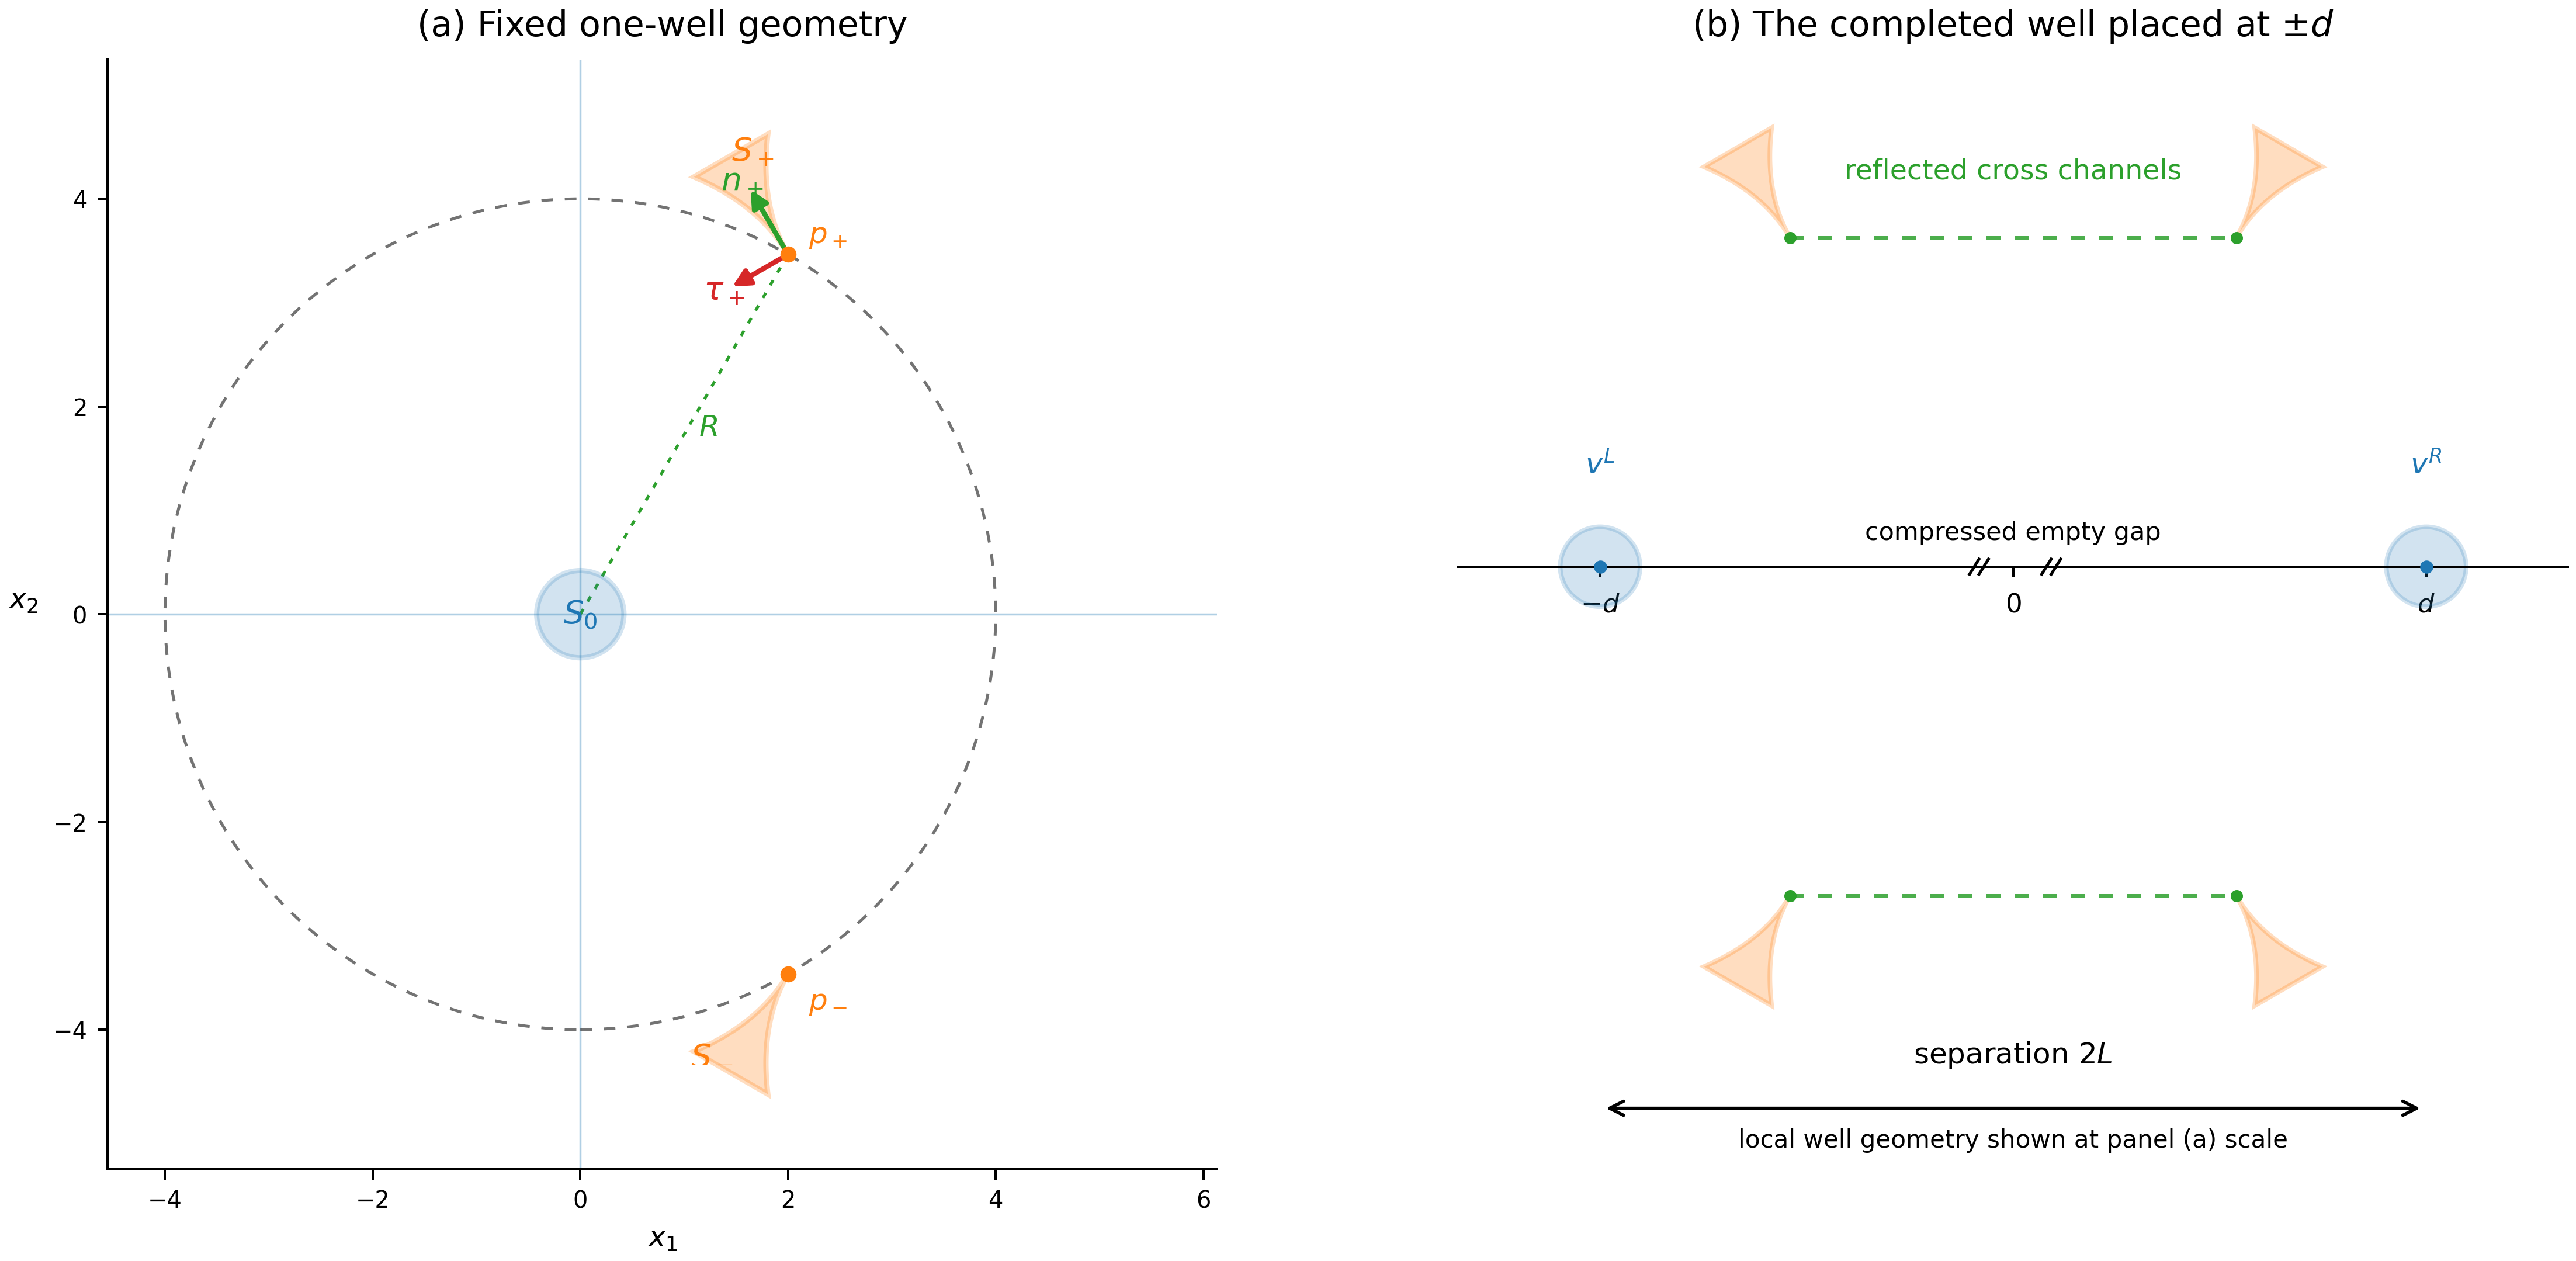
\includegraphics[width=\textwidth]{figures/figure1_fixed_cusp_geometry.png}
\caption{Geometry of the construction.  The radial core and the two
one-sided cusps are fixed before the separation is chosen.  Their tips
are the unique rightmost points of the cusp supports, while the outgoing
normal directions have strictly positive radial components.  The completed one-well potential is then placed at the two center $\pm d$, with separation $2L$.}
\label{fig:fixed-cusp-geometry}
\end{figure}
Note additionally that $p_\pm\cdot n_\pm=R/2$ and
$|\det(n_\pm,\tau_\pm)|=1$.  In particular, the directions $n_\pm$
point radially outward while their first components are negative.

\subsection{Double-well potential}

Let $d=(L,0)$.  We later impose stricter bound on $L > L_0(R)$, but in particular $2L>R$ ensures
\[
 p_++p_--2d=(R-2L,0)
\]
has negative first component.
To encode the cross-cusp channel that will later produce the leading hopping term, introduce its magnetic phase and corresponding total action by
\begin{equation}\label{eq:Phi}
 \Phi(z,w)=b\left[d\wedgep(z-w)+\frac12z\wedgep w\right]
\end{equation}
and
\begin{equation}\label{eq:A0-new}
 g_0(z)=\cJ_1(|z|),
 \qquad
 \cA_0(z,w)=g_0(z)+g_0(w)+\cJ_1(|z+w-2d|).
\end{equation} 
The normal action and phase slopes at the cross pair are
\begin{align}
m_R&:=\partial_{n_+}g_0(p_+){,}
\label{eq:mR_0}\\
 j&:=\partial_{n_+}\cJ_1(|z+w-2d|)\big|_{(p_+,p_-)}{,}
      \label{eq:j-new_0}\\
\alpha&:=\partial_{n_+}\cA_0(p_+,p_-){,}
 \label{eq:alpha-new_0}\\
\theta&:=\partial_{n_+}\Phi(p_+,p_-){.}
 \label{eq:theta-new_0}
\end{align}
The reflected $w$ derivatives have the same values.  The active phase is
\begin{equation}\label{eq:Phi-star}
 \Phi_*:=\Phi(p_+,p_-{).}
\end{equation}
The
quadratic cusp introduced below makes every
tangential displacement $O(t^2)$, while the outgoing action grows linearly in
$t$.

\begin{proposition}[Geometric certificate]\label{prop:geometry-certificate}
The geometry \Cref{eq:fixed-tips}--\Cref{eq:fixed-frames} has the following
properties.
\begin{enumerate}[label=\textup{(\roman*)},leftmargin=2.5em]
\item The {following} identities hold
{\begin{align}
m_R&=\frac12\cJ_1'(R)>0,\label{eq:mR}\\
 j&=\frac12\cJ_1'(2L-R)>0,\label{eq:j-new}\\
 \alpha&=m_R+j,\label{eq:alpha-new}\\
 \theta&=\frac{\sqrt3}{2}bL>0.\label{eq:theta-new}
\end{align}
}and
$\alpha-i\theta$ lies in the open right half-plane.
\item For every $\cE>0$, the same-cusp bridge gap at the tips satisfies
\begin{equation}\label{eq:same-tip-gap}
 \cJ_\cE\!\left(\sqrt{(2L-R)^2+3R^2}\right)-\cJ_\cE(2L-R)
 \ge \frac{3bR^2}{4}.
\end{equation}
\item Put
\[
 \delta_{\rm cp}:=\frac R2-r_0>0,
 \qquad
 \delta_{\rm cc}:=R-2r_0>0.
\]
The two quantities
\begin{align*}
 &\cJ_1(2L-R+\delta_{\rm cp})-\cJ_1(2L-R)-\cJ_1(R),\\
 &\cJ_1(2L-R+\delta_{\rm cc})-\cJ_1(2L-R)-2\cJ_1(R)
\end{align*}
are strictly increasing for $L>R/2$ and tend to $+\infty$ as
$L\to\infty$.
\end{enumerate}
\end{proposition}

\begin{proof}
The radial identities follow from
$p_+/R=(1/2,\sqrt3/2)$ and
$p_+\cdot n_+=R/2$.  Since the bridge vector at the cross pair is
$(R-2L,0)$, its gradient in the $z$ variable is
$-\cJ_1'(2L-R)e_1$, whose scalar product with $n_+$ is
$\cJ_1'(2L-R)/2$.  This proves \Cref{eq:mR}--\Cref{eq:alpha-new}.
Direct differentiation of \Cref{eq:Phi} gives
\[
 \nabla_z\Phi(p_+,p_-)
 =b\left(-\frac{\sqrt3R}{4},L-\frac R4\right),
\]
and its scalar product with $n_+$ is $\sqrt3bL/2$.  A direct wedge-product
calculation gives \Cref{eq:Phi-star}.

For $s>0$,
\[
 \frac{\dd}{\dd s}\cJ_\cE(\sqrt s)
 =\frac{1}{4}\sqrt{b^2+\frac{4\cE}{s}}
 \ge\frac b4.
\]
The two squared bridge lengths in \Cref{eq:same-tip-gap} differ by
$3R^2$, proving that inequality.

Finally, $\cJ_1'$ is strictly increasing.  Hence, for every fixed
$\delta>0$, the function
$D\mapsto\cJ_1(D+\delta)-\cJ_1(D)$ is strictly increasing.  Also
\[
 \cJ_1(D+\delta)-\cJ_1(D)
 \ge\frac b4\bigl((D+\delta)^2-D^2\bigr)
 \longrightarrow+\infty.
\]
This proves the last assertion.

\begin{formalisationaddition}{P2.6}
Let $D=2L-R>0$. The calculations below use only the coordinates in \eqref{eq:fixed-tips}--\eqref{eq:fixed-frames} and the action derivative from Proposition 2.2.

\begin{lemma}[Normal derivatives of the two real actions]\label{sublemma:P2-6-action-slopes}
At the upper and lower tips,
\[
 p_\sigma\cdot n_\sigma=R/2,\qquad
 \partial_{n_\sigma}\cJ_1(|z|)\big|_{p_\sigma}=\cJ_1'(R)/2=m_R.
\]
At $(p_+,p_-)$ the derivative of $\cJ_1(|z+w-2d|)$ in either outgoing normal variable is $\cJ_1'(D)/2=j$.
\end{lemma}
\begin{proof}
For the upper tip the dot product is $-R/4+3R/4=R/2$; reflection preserves it. The differential of $|z|$ is $z/|z|$, so its scalar product with the outgoing normal is $1/2$.
At the cross pair, $z+w-2d=(-D,0)$. The gradient of its norm in either variable is $(-1,0)$. Both normals have first coordinate $-1/2$, so the scalar product is again $1/2$. This proves the two action derivatives and their sum $\alpha=m_R+j>0$.
\end{proof}

\begin{lemma}[Magnetic phase, its sign, and its two slopes]\label{sublemma:P2-6-phase-calculation}
Writing $\Phi=b[L(z_2-w_2)+(z_1w_2-z_2w_1)/2]$, one has
\[
 \Phi(p_+,p_-)=\sqrt3\,bR(L-R/4)=\Phi_*,\qquad
 \partial_{n_+}^{z}\Phi=\partial_{n_-}^{w}\Phi=\sqrt3\,bL/2=\theta
\]
at the cross pair. In particular $\alpha-i\theta$ is in the open right half-plane.
\end{lemma}
\begin{proof}
Here $d\wedge(p_+-p_-)=\sqrt3LR$ and
$p_+\wedge p_-=-\sqrt3R^2/2$, which gives the value.
The two gradients are
\[
 \nabla_z\Phi=b(w_2/2,L-w_1/2),\qquad
 \nabla_w\Phi=b(-z_2/2,-L+z_1/2).
\]
At the tips these become $b(-\sqrt3R/4,L-R/4)$ and
$b(-\sqrt3R/4,-L+R/4)$. Their dot products with
$(-1/2,\sqrt3/2)$ and $(-1/2,-\sqrt3/2)$ are both
$\sqrt3bR/8+\sqrt3bL/2-\sqrt3bR/8=\sqrt3bL/2$.
The real part of $\alpha-i\theta$ is $\alpha>0$.
\end{proof}

\begin{lemma}[Same-cusp bridge penalty]\label{sublemma:P2-6-same-cusp}
The squared bridge lengths at a same-cusp pair and a cross pair differ by $3R^2$. Their actions therefore differ by at least $3bR^2/4$ for every $E>0$.
\end{lemma}
\begin{proof}
One has $2p_+-2d=(-D,\sqrt3R)$, whereas $p_++p_--2d=(-D,0)$. Their squared lengths are $D^2+3R^2$ and $D^2$. Integrate
$\frac{\mathrm d}{\mathrm ds}\cJ_E(\sqrt s)\ge b/4$ from $D^2$ to $D^2+3R^2$. Reflection gives the lower same-cusp pair. This proves \eqref{eq:same-tip-gap}.
\end{proof}

\begin{lemma}[Increasing and unbounded fixed-displacement reserves]\label{sublemma:P2-6-displacement}
For every fixed $\delta>0$, the function
$D\mapsto \cJ_1(D+\delta)-\cJ_1(D)$ is strictly increasing on $(0,\infty)$ and tends to $+\infty$.
\end{lemma}
\begin{proof}
Its derivative is $\cJ_1'(D+\delta)-\cJ_1'(D)>0$ because $\cJ_1''>0$. Also $\cJ_1'(r)\ge br/2$, so
\[
 \cJ_1(D+\delta)-\cJ_1(D)\ge\frac b4((D+\delta)^2-D^2)
 =\frac{b\delta}{2}D+\frac{b\delta^2}{4}\longrightarrow\infty.
\]
\end{proof}
\finish The two displacements in the proposition are positive since $R>8r_0$: $\delta_{cp}=R/2-r_0>0$ and $\delta_{cc}=R-2r_0>0$. Apply the last sublemma and subtract respectively the fixed numbers $\cJ_1(R)$ and $2\cJ_1(R)$. Since $D=2L-R$ is strictly increasing in $L$, all assertions follow. These are estimates uniform for all later larger displacements; none requires choosing a new cusp profile.
\end{formalisationaddition}

\end{proof}

\subsection{The fixed log-flat cusp profile and the
\texorpdfstring{$h\log(1/h)$}{h log(1/h)} scale}\label{ssec:construction}

The cusp must be fixed independently of $h$, while its leading contribution
must concentrate near its tip.  The log-flat profile used below has this
property and separates the incoming channel from the exact scattered
response in the geometry considered here.
Fix $t_*>0$ and define
\begin{equation}\label{eq:log-flat-function}
 \ell(t):=\log\frac{t_*}{t},
 \qquad 0<t<t_*.
\end{equation}

\subsubsection{Log-flat balance}

\begin{lemma}[Log-flat minimum]\label{lem:flat-min}
Let $A,\beta>0$ and $0<h<1$.  The function
\[
 t\longmapsto \beta\ell(t)^2+\frac{At}{h}
\]
has a unique critical point in $(0,t_*)$, given for small $h$ by
\begin{equation}\label{eq:log-flat-saddle-real}
 t_{A,h}=\frac{2\beta h}{A}
 W_0\!\left(\frac{At_*}{2\beta h}\right),
\end{equation}
where $W_0$ is the principal Lambert function.  At this point the minimum is
\begin{equation}\label{eq:log-flat-minimum}
 \beta\left(W_0\!\left(\frac{At_*}{2\beta h}\right)^2
 +2W_0\!\left(\frac{At_*}{2\beta h}\right)\right).
\end{equation}
In particular,
\begin{equation}\label{eq:log-flat-scale}
 t_{A,h}\asymp_A h\log(1/h),
 \qquad
 \min\left(\beta\ell(t)^2+\frac{At}{h}\right)
 =\beta\log^2(1/h)+O_A\bigl(\log(1/h)\log\log(1/h)\bigr).
\end{equation}
\end{lemma}

\begin{proof}
The critical-point equation is
\[
 \frac{At}{h}=2\beta\ell(t).
\]
Writing $w=\ell(t)$ and $t=t_*e^{-w}$ gives
$we^w=At_*/(2\beta h)$, which proves
\Cref{eq:log-flat-saddle-real}.  Substitution gives
\Cref{eq:log-flat-minimum}.  The standard expansion
$W_0(x)=\log x-\log\log x+O(1)$ proves
\Cref{eq:log-flat-scale}.

\begin{formalisationaddition}{L2.7}
\begin{lemma}[Convexity and the Lambert equation]\label{sublemma:L2-7-stationary}
For $f(t)=\beta\log^2(t_*/t)+At/h$ on $(0,t_*)$, one has
\[
 f'(t)=A/h-2\beta\ell(t)/t,\qquad
 f''(t)=2\beta(1+\ell(t))/t^2>0.
\]
Its unique critical point satisfies $t_A=(2\beta h/A)w$, where
$w>0$ solves $we^w=At_*/(2\beta h)$.
\end{lemma}
\begin{proof}
Differentiate using $\ell'(t)=-1/t$. The first derivative tends to $-\infty$ at zero and to $A/h>0$ at $t_*$. Strict convexity gives a unique minimum. If $w=\ell(t_A)>0$, the equation $f'(t_A)=0$ is $At_A/h=2\beta w$. Substitute $t_A=t_*e^{-w}$ to obtain $we^w=At_*/(2\beta h)$. The function $w\mapsto we^w$ is strictly increasing on $(0,\infty)$, with range $(0,\infty)$; its positive inverse is $W_0$. This proves \eqref{eq:log-flat-saddle-real}.
\end{proof}

\begin{lemma}[Minimum and elementary logarithmic scale]\label{sublemma:L2-7-value-scale}
At this critical point $f(t_A)=\beta(w^2+2w)$. If $A$ ranges in a compact subset of $(0,\infty)$, then
$w=\log(1/h)+O(\log\log(1/h))$ uniformly.
\end{lemma}
\begin{proof}
Insert $\ell(t_A)=w$ and $At_A/h=2\beta w$ in $f$.
Put $X=At_*/(2\beta h)$. For $X$ large, the equation $w+\log w=\log X$ gives
$\log X-\log\log X\le w\le\log X$; the lower bound follows by substituting $w\le\log X$ back into that equation. Uniform compact bounds on $A$ give $\log X=\log(1/h)+O(1)$. It follows that $t_A$ is bounded above and below by positive constants times $h\log(1/h)$ and
$\beta(w^2+2w)=\beta\ell_h^2+O(\ell_h\log\ell_h)$.
\end{proof}
\finish These are precisely \eqref{eq:log-flat-minimum}--\eqref{eq:log-flat-scale}. In particular the minimizer tends to zero and eventually lies in every fixed interval on which a cutoff equals one.
\end{formalisationaddition}

\end{proof}

\begin{lemma}[Real log-flat integral bounds]\label{lem:log-flat-L1}
Fix $k\in\R$, $0<t_0<t_*$, and a compact interval
$I_A\Subset(0,\infty)$.  Let
$\chi\in C_c^\infty((-t_*/2,t_0);[0,1])$ be equal to one near $t=0$.
For every $\eta>0$ there is $h_\eta>0$ such that, uniformly
for $A\in I_A$ and $0<h<h_\eta$,
\begin{equation}\label{eq:log-flat-integral-bounds}
 e^{-(\beta+\eta)\log^2(1/h)}
 \le
 \int_0^{t_0}t^k\chi(t)
 e^{-\beta\ell(t)^2-At/h}\dd t
 \le
 e^{-(\beta-\eta)\log^2(1/h)}.
\end{equation}
The same upper bound holds after multiplication by any fixed power of
$\ell(t)$ or $t^{-1}$.
\end{lemma}

\begin{proof}
The flat factor makes the integral finite for every fixed $k$.  The minimum
in \Cref{lem:flat-min} and the expansion
\Cref{eq:log-flat-scale} give the upper bound after splitting into a fixed
neighborhood of $t_{A,h}$ and its complement.  For the lower bound, integrate
over an interval of length $ct_{A,h}/\sqrt{\log(1/h)}$ centered at
$t_{A,h}$; the second derivative of the exponent there is
$O((h^2\log(1/h))^{-1})$, so the exponent increases by only $O(1)$.
All powers of $t_{A,h}^{\pm1}$ and $\ell(t_{A,h})$ contribute only
$O(\log(1/h))$ to the logarithm and are absorbed by $\eta\log^2(1/h)$.
Uniformity follows from compactness of $I_A$.

\begin{formalisationaddition}{L2.8}
It suffices to prove logarithmic asymptotics up to $o(\ell_h^2)$, uniformly for $A$ in its stated compact interval. The cutoff is bounded, nonnegative, and equals one near zero, as in the statement.

\begin{lemma}[Integrability and polynomial factors]\label{sublemma:L2-8-integrability}
For any real $k$ and fixed nonnegative integer $m$, the function
$t^k(1+\ell(t))^m e^{-\beta\ell(t)^2}$ is integrable near zero. Fixed extra powers of $t$ or $\ell(t)$ do not change the leading coefficient of $\ell_h^2$ in the logarithm of the integral below.
\end{lemma}
\begin{proof}
Use $y=\log(t_*/t)$ and $\mathrm dt=-t_*e^{-y}\mathrm dy$. The resulting factor is
$t_*^{k+1}(1+y)^m e^{-\beta y^2-(k+1)y}$, whose Gaussian decay makes it integrable for every real $k$. For every $\epsilon>0$, the linear term and $m\log(1+y)$ have modulus at most $\epsilon y^2+C_\epsilon$. This observation will also absorb them in the following upper bound; the lower-bound calculation treats them directly at the saddle scale.
\end{proof}

\begin{lemma}[Upper log-flat estimate]\label{sublemma:L2-8-upper}
For every $\eta>0$, uniformly in the given slopes,
\[
 \int_0^{t_0}t^k(1+\ell(t))^m e^{-\beta\ell(t)^2-At/h}\,\mathrm dt
 \le e^{-(\beta-\eta)\ell_h^2}
\]
for all sufficiently small $h$, after multiplication by any fixed bounded cutoff or fixed constant.
\end{lemma}
\begin{proof}
Fix small $\epsilon,\delta>0$ so that $(\beta-\epsilon)(1-\delta)^2>\beta-\eta/2$; when $\eta\ge\beta$ it is enough to prove a stronger estimate with a smaller positive $\eta$. In the $y$ variable, split at $Y=(1-\delta)\ell_h$.
For $y\ge Y$, discard $e^{-At_*e^{-y}/h}\le1$ and absorb the polynomial/linear factors into $e^{\epsilon y^2}$ as above. The elementary Gaussian tail estimate
$\int_Y^\infty e^{-c y^2}\mathrm dy\le e^{-cY^2}/(2cY)$ gives the desired bound with room in the exponent.
For $y_0=\log(t_*/t_0)\le y\le Y$, one has $At_*e^{-y}/h\ge A_{\min}t_*e^{\delta\ell_h}$. On this interval the remaining integrand is bounded by $C e^{C\ell_h}(1+\ell_h)^m$; the interval has length $O(\ell_h)$. The factor $\exp[-A_{\min}t_*e^{\delta\ell_h}]$ dominates $\exp[-M\ell_h^2]$ for every fixed $M$. Absorb constants and the two summands in the unused $\eta\ell_h^2/2$ margin.
\end{proof}

\begin{lemma}[Lower log-flat estimate on an explicit interval]\label{sublemma:L2-8-lower}
If $\chi=1$ near zero, then for every $\eta>0$,
\[
 \int_0^{t_0}t^k\chi(t)e^{-\beta\ell(t)^2-At/h}\,\mathrm dt
 \ge e^{-(\beta+\eta)\ell_h^2}
\]
uniformly in the stated slopes for small $h$.
\end{lemma}
\begin{proof}
Let $t_A$ be the preceding real minimizer and $w=\ell(t_A)\asymp\ell_h$. Integrate only over
$[t_A,t_A(1+w^{-1/2})]$, which lies where $\chi=1$ for small $h$. On this interval $t\asymp t_A$, and
$f''(t)\le Cw/t_A^2$. Since $f'(t_A)=0$, Taylor's integral formula gives $f(t)\le f(t_A)+C$ there. The interval length is $t_Aw^{-1/2}$, and $t^k\ge c_k t_A^k$. Hence the integral is at least
$c_k t_A^{k+1}w^{-1/2}e^{-f(t_A)-C}$.
Its logarithm is
$-\beta\ell_h^2+O(\ell_h\log\ell_h)$: use Lemma 2.7, $\log t_A=-\ell_h+O(\log\ell_h)$, and $\log w=O(\log\ell_h)$. The error is smaller than $\eta\ell_h^2$ for small $h$.
\end{proof}
\finish The upper and lower sublemmas give \eqref{eq:log-flat-integral-bounds}. An extra fixed negative power of $t$ is handled by replacing $k$ with another real number. An extra power of $\ell(t)$ is handled by the first two sublemmas. This proves the stated stability of the upper bound without restricting $k$ to be greater than $-1$.
\end{formalisationaddition}

\end{proof}

\subsubsection{Definition and admissibility of the exterior cusp components}

Choose $0<t_0<t_*$ and $s_0>0$.  Define
\begin{equation}\label{eq:chart}
 \Psi_+(t,s)=p_++tn_++t^2s\tau_+,
 \qquad
 \Psi_-(t,s)=\cR\Psi_+(t,s),
 \qquad 0< t<t_0,
 \quad |s|<s_0.
\end{equation}
Each map extends continuously to $t=0$, where the entire edge
$\{0\}\times(-s_0,s_0)$ collapses to the corresponding tip.  Thus
``embedding'' below always refers to the open strip $t>0$ {and, in particular,} the collapsed edge
belongs to the cusp closure, not to the embedding domain.

\begin{figure}[t]
    \centering
    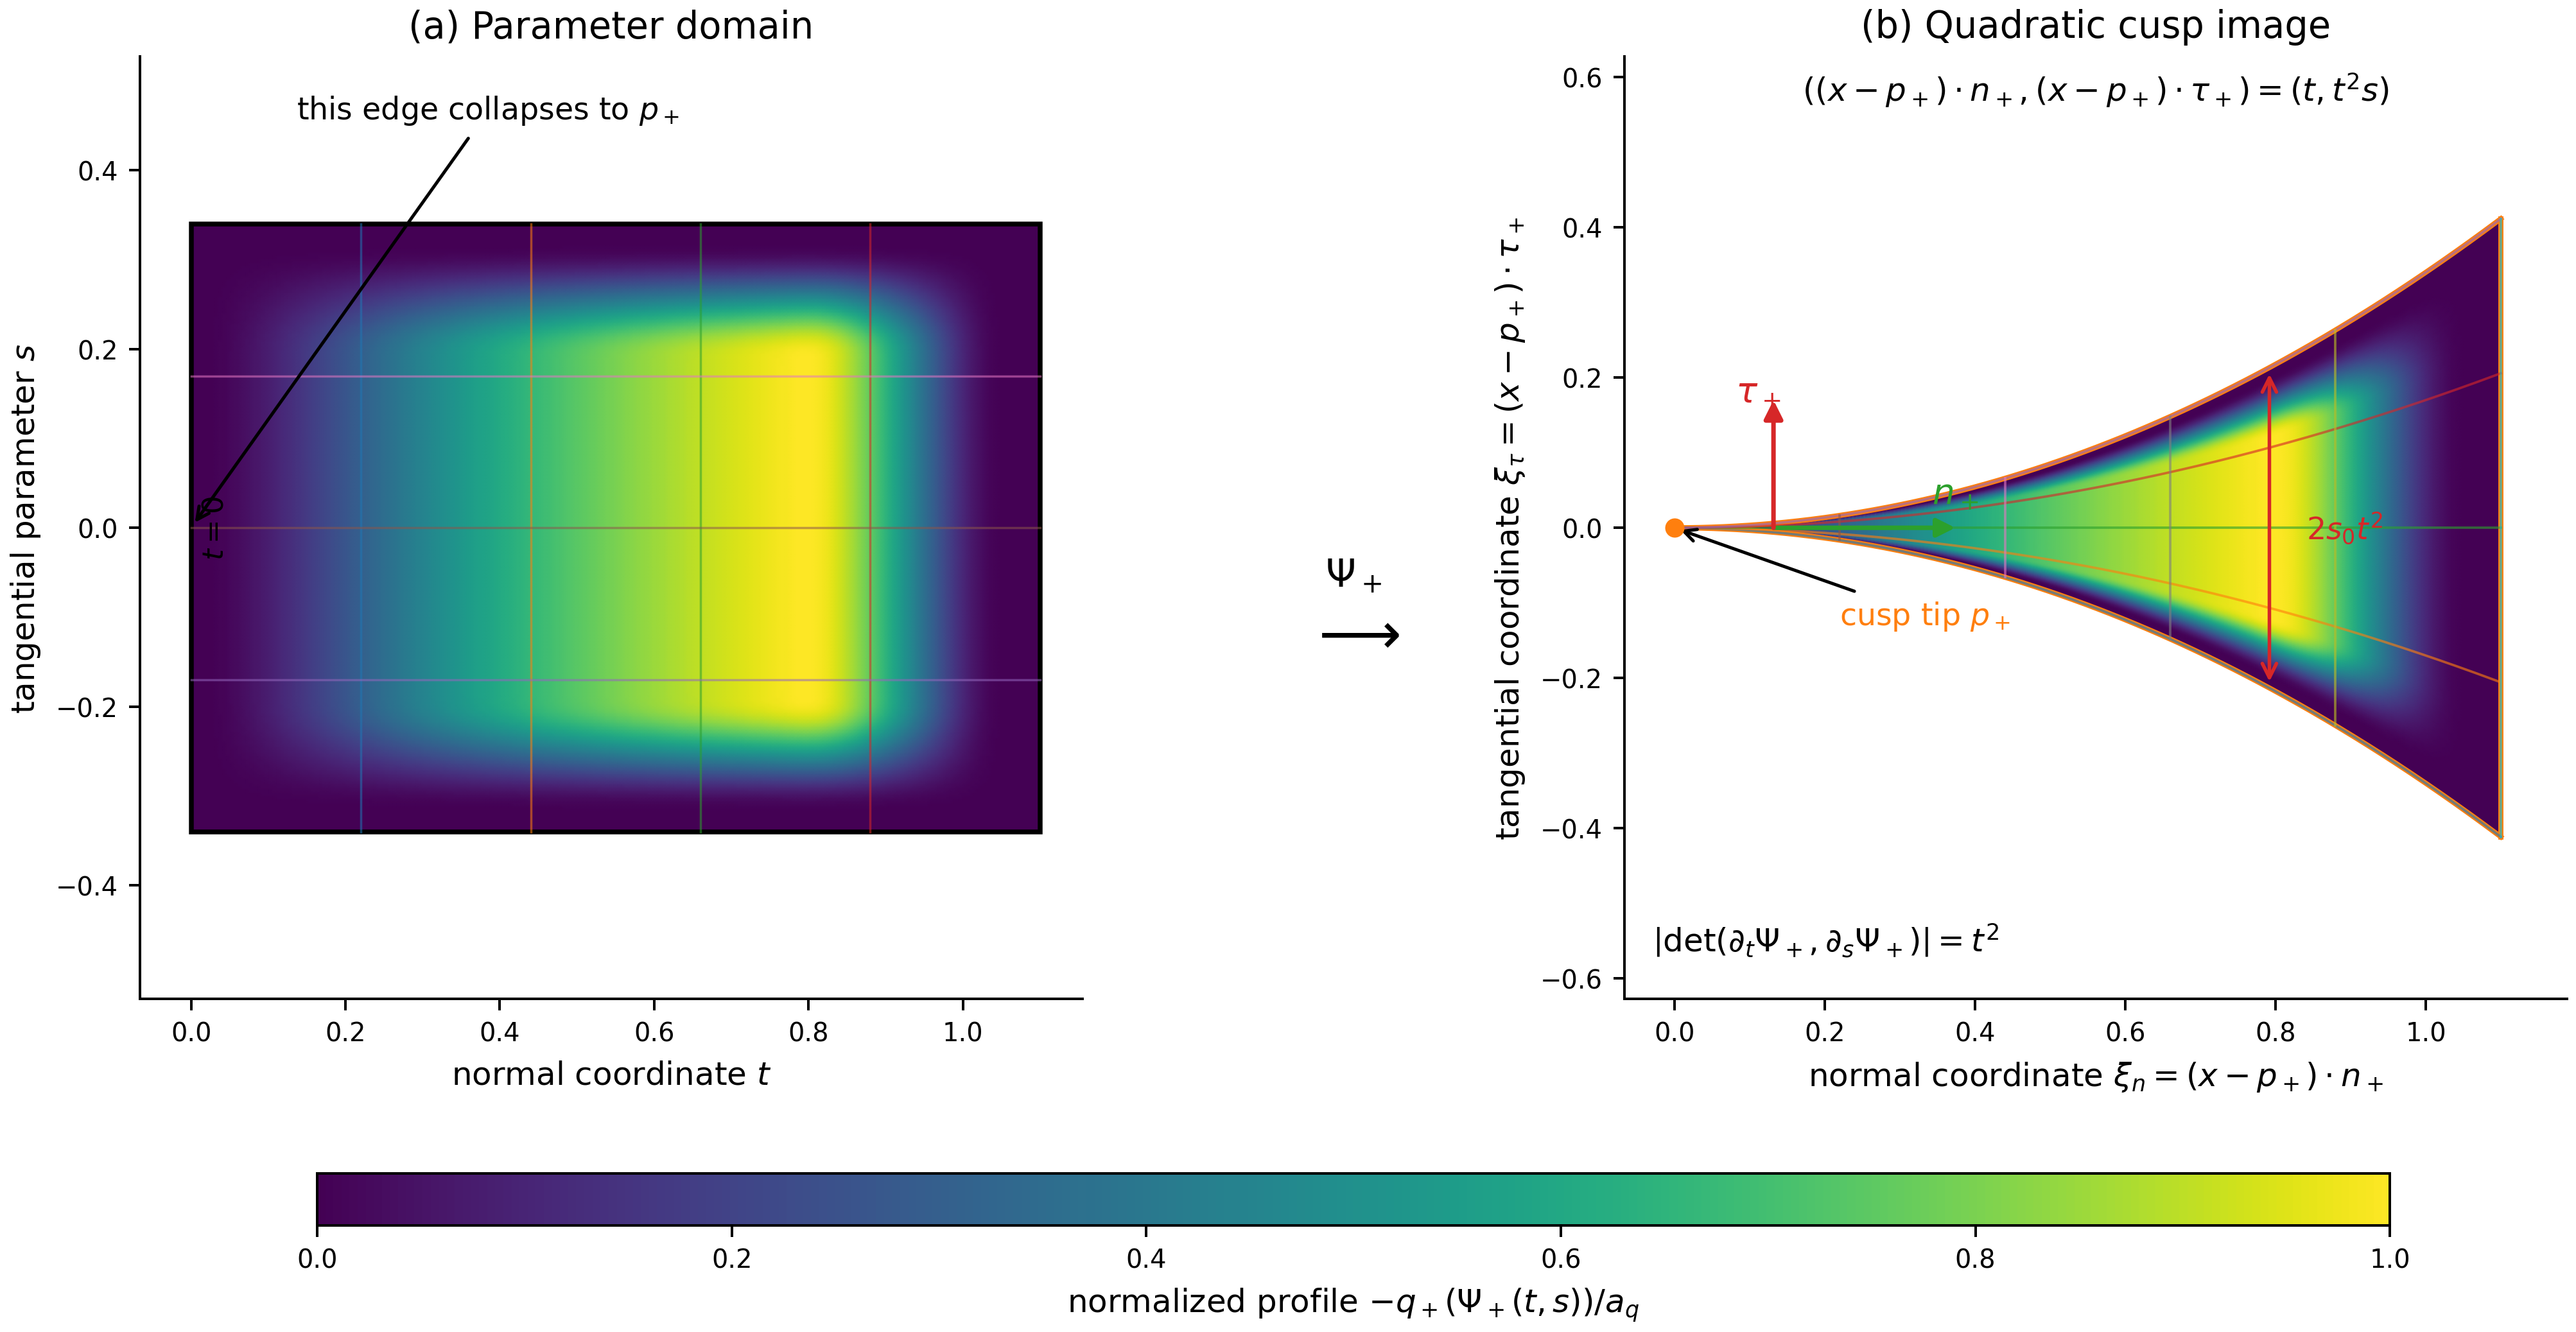
\includegraphics[width=\linewidth]{figures/figure2_quadratic_cusp_chart.png}
    \caption{The quadratic cusp chart. The parameter domain $0<t<t_0$, $s<s_0$ is mapped by $\Psi_+(t,s)=p_++tn_++t^2s\tau_+$. The edge $t=0$ collapses to the cusp tip $p_+$, while a section at fixed $t$ has width $2s_0t^2$ in the $\tau_+$ direction. Consequently $|\det(\partial_t\Psi_+, \partial_s\Psi_+)|=t^2$. The shading displays a representative normalized log-flat cusp profile.}
    \label{fig:quadratic-cusp-chart}
\end{figure}

The absolute Jacobian is exactly
\begin{equation}\label{eq:cusp-jacobian}
 \left|\det(\partial_t\Psi_\pm,\partial_s\Psi_\pm)\right|=t^2.
\end{equation}
Choose $\chi_a\in C_c^\infty((-t_*/2,t_0);[0,1])$ with
$\chi_a\equiv1$ on $[0,t_2]$ for some $0<t_2<t_0$, and choose an even
$\chi_b\in C_c^\infty((-s_0,s_0);[0,1])$, equal to one on
$[-s_0/2,s_0/2]$, with $\int\chi_b>0$.  For $a_q,\beta>0$, define
\begin{equation}\label{eq:cusp-def}
 q_+(\Psi_+(t,s))
 =-a_qe^{-\beta\ell(t)^2}\chi_a(t)\chi_b(s),
 \qquad t>0,
\end{equation}
set $q_+=0$ outside the chart image, and put $q_-=q_+\circ\cR$.  The final
one-well potential is
\begin{equation}\label{eq:final-v}
 v=v^\circ+\eps(q_++q_-).
\end{equation}
We impose
\begin{equation}\label{eq:epsilon-small}
 \eps a_q\le\delta_0<\frac14.
\end{equation}

\begin{lemma}[Smoothness, one-sidedness, and admissibility]
\label{lem:smooth-new}
After decreasing $s_0$ and $t_0$, the restrictions of $\Psi_\pm$ to
$(0,t_0)\times(-s_0,s_0)$ are embeddings with mutually disjoint images
disjoint from $\supp v^\circ$, and they extend continuously to their collapsed
tip edges.  The functions
$q_\pm$ belong to $C_c^\infty(\R^2)$ and are flat at their tips.  Moreover,
there are constants $c_x,c_r>0$ such that on either cusp support
\begin{align}
 (\Psi_\pm(t,s))_1&\le \frac R2-c_xt,\label{eq:one-sided-x}\\
 |\Psi_\pm(t,s)|&\ge R+c_rt.\label{eq:radial-outward}
\end{align}
On the upper cusp $(\Psi_+(t,s))_2\ge\sqrt3R/2$, and on the lower cusp
$(\Psi_-(t,s))_2\le-\sqrt3R/2$.  Consequently the potential
\Cref{eq:final-v} is smooth, compactly supported, nonpositive,
nonradial, invariant under $\cR$, and has the same unique nondegenerate
minimum as $v^\circ$.
\end{lemma}

\begin{proof}
In the orthonormal frame $(n_+,\tau_+)$, the chart coordinates of
$\Psi_+(t,s)-p_+$ are $(t,t^2s)$.  On $t>0$ the map
$(t,s)\mapsto(t,t^2s)$ has inverse $(t,\sigma)\mapsto(t,\sigma/t^2)$, hence
$\Psi_+$ is an embedding there, and \Cref{eq:cusp-jacobian} follows.  The
reflected chart has the same absolute Jacobian.  The continuous extension to
$t=0$ and collapse of the edge follow directly from the formula.  Since the
tips and the core are separated, shortening the charts makes the open images
disjoint.

Every Cartesian derivative of
$e^{-\beta\ell(t)^2}\chi_b(s)$, after it is expressed through the inverse
chart, is bounded by
\[
 C_Nt^{-N}(1+\ell(t))^N e^{-\beta\ell(t)^2}.
\]
This tends to zero faster than every power of $t$.  The extension by zero is
therefore smooth and flat at the tip.  The compact supports of the cutoffs
handle the other chart boundaries.

Using \Cref{eq:fixed-frames},
\[
 (\Psi_+(t,s))_1-\frac R2
 =-\frac t2-\frac{\sqrt3}{2}t^2s.
\]
For $\sqrt3s_0t_0\le1/2$, this is at most $-t/4$.  Moreover, orthonormality of $(n_+,\tau_+)$ and the fixed scalar products
with $p_+$ give the exact identity
\[
 |\Psi_+(t,s)|^2
 =R^2+Rt+(1-\sqrt3Rs)t^2+s^2t^4.
\]
If $s\le0$ the mixed correction is nonnegative.  If $s>0$, the condition
$\sqrt3s_0t_0\le1/2$ gives $\sqrt3st\le1/2$.  In both cases the right side is
at least $(R+t/4)^2$, and hence $|\Psi_+(t,s)|\ge R+t/4$.  Finally,
\[
 (\Psi_+(t,s))_2-\frac{\sqrt3R}{2}
 =\frac{\sqrt3}{2}t-\frac12t^2s\ge0
\]
when $s_0t_0\le\sqrt3$.  Reflection gives the lower-cusp statements.  The two packets are smooth,
nonpositive, nonzero, reflection-related, and supported away from the core and
from one another.  Their depth is at most $\delta_0<1/4$, whereas the unique
core minimum has value $-1$ and is unchanged in a neighborhood.  Thus no new
global minimum is introduced, and the packet geometry makes the sum
nonradial.  The remaining assertions about $v$ follow from the same support
separation and \Cref{eq:final-v}.

\begin{formalisationaddition}{L2.9}
All reductions of $s_0,t_0$ in this proof take place during construction of the potential, before it is fixed and before $L$ is chosen.

\begin{lemma}[Chart inverse and exact Jacobian]\label{sublemma:L2-9-chart-calculus}
In the orthonormal frame $(n_+,\tau_+)$, the chart is $(t,s)\mapsto(t,t^2s)$. On $t>0$ it is injective, its inverse is $(u,v)\mapsto(u,v/u^2)$, and its absolute Jacobian is $t^2$. In these coordinates
\[
 \partial_u=\partial_t-(2s/t)\partial_s,\qquad
 \partial_v=t^{-2}\partial_s.
\]
\end{lemma}
\begin{proof}
Equality of first coordinates gives equality of $t$; since $t^2>0$, equality of second coordinates then gives equality of $s$. The derivative matrix is
$\left(\begin{smallmatrix}1&0\\2ts&t^2\end{smallmatrix}\right)$ and has determinant $t^2$. An orthonormal change of frame has determinant of modulus one, so the absolute Cartesian Jacobian is the same. Differentiate $t=u$ and $s=v/u^2$ to obtain the two differential operators. Reflection has absolute determinant one and gives the identical conclusions for the lower chart. This proves \eqref{eq:cusp-jacobian}, independently of any smoothness assertion at the tip.
\end{proof}

\begin{lemma}[Flatness dominates all chart singularities]\label{sublemma:L2-9-flat-extension}
For every integer $m\ge0$, every Cartesian derivative of $q_+$ of order at most $m$ in its chart is bounded by
$C_m t^{-N_m}(1+\ell(t))^{N_m}e^{-\beta\ell(t)^2}$ for some $N_m$. This bound tends to zero faster than every power of the distance to the tip as $t\downarrow0$.
\end{lemma}
\begin{proof}
The derivative of $e^{-\beta\ell^2}$ is $(2\beta\ell/t)e^{-\beta\ell^2}$. Repeated differentiation therefore gives that exponential times a polynomial in $\ell$ and inverse powers of $t$. The chart differential operators in the preceding sublemma add only further such factors; derivatives of the compactly supported cutoffs are bounded. Induction on $m$ gives the bound.
Write $t=t_*e^{-y}$. For every fixed $N,M$, the logarithm of
$t^{-N-M}(1+\ell)^N e^{-\beta\ell^2}$ equals $-\beta y^2+(N+M)y+N\log(1+y)+O(1)$, which tends to $-\infty$. Also
$|\Psi_+(t,s)-p_+|=t\sqrt{1+t^2s^2}\asymp t$ on the fixed parameter rectangle.
At lateral and outer chart boundaries the cutoffs vanish on neighborhoods, so zero extension is smooth there. At the tip all derivatives tend to zero with the bounds just proved. To justify extension rather than only formal limits, extend each derivative by zero and use the difference quotient estimate $|D^\alpha q(x)|=o(|x-p_+|)$; induct on $|\alpha|$. This gives a $C^\infty$ extension with every derivative zero at the tip. The same argument applies after reflection.
\end{proof}

\begin{lemma}[Explicit one-sided coordinate inequalities]\label{sublemma:L2-9-coordinate-inequalities}
By taking $s_0t_0$ sufficiently small, for both signs and all chart points,
$x_1\le R/2-t/4$ and $|x|\ge R+t/4$. For the upper chart $x_2\ge\sqrt3R/2$, and the lower inequality is its reflection.
\end{lemma}
\begin{proof}
Direct substitution gives
\[
 x_1=R/2-t/2-\sqrt3t^2s/2,\qquad
 x_2=\sqrt3R/2+\sqrt3t/2-t^2s/2,
\]
\[
 |x|^2=R^2+Rt+(1-\sqrt3Rs)t^2+s^2t^4.
\]
Require $\sqrt3s_0t_0\le1/2$ and $s_0t_0\le\sqrt3$.
Then $x_1\le R/2-t/4$ and $x_2\ge\sqrt3R/2$.
Moreover
\[
 |x|^2-(R+t/4)^2
 =Rt/2-\sqrt3Rs t^2+(15/16)t^2+s^2t^4\ge0,
\]
since $\sqrt3s t\le1/2$. Both radii are nonnegative, so taking square roots proves the radial inequality. These yield \eqref{eq:one-sided-x}--\eqref{eq:radial-outward}, with $c_x=c_r=1/4$ if desired.
\end{proof}

\begin{lemma}[Support separation and admissibility]\label{sublemma:L2-9-potential}
The supports of the core and the two cusp components are pairwise disjoint for sufficiently small fixed chart parameters. The resulting $v$ belongs to $C_c^\infty(\R^2;[-1,0])$, has the same unique minimum and Hessian as $v^\circ$, is reflection-symmetric, and is not radial.
\end{lemma}
\begin{proof}
The tips are at radius $R>r_0$, are distinct, and are separated from the core by a positive distance. The chart displacements have length at most $t_0\sqrt{1+t_0^2s_0^2}$, so take this length smaller than one third of the relevant distances. Smoothness follows from the flat-extension sublemma. Since the supports are disjoint, at most one of $v^\circ,\eps q_+,\eps q_-$ is nonzero at a point. The core takes values in $[-1,0]$ and the cusp depths are at most $\eps a_q\le\delta_0<1$, because the cutoffs are chosen between zero and one. Thus no new minimum of value $-1$ is created; near zero nothing is changed. The definition $q_-=q_+\circ R$ gives the reflection symmetry.
Finally choose a point in the interior of the upper cusp where both cutoffs are positive. At its radius, larger than $r_0$, there is an angular point outside the two short cusp neighborhoods. The potential is negative at the first and zero at the second. Therefore it is not radial.
\end{proof}
\finish The chart, flatness, one-sidedness and support assertions of the lemma all follow. The proof also specifies how all inequalities can be made strict before fixing the final potential.
\end{formalisationaddition}

\end{proof}

\subsection{Outgoing-cusp control}\label{sec:outgoing-cusp}
To condense notation, we introduce
\[
g_h(x) := \cJ_{\cE^\circ_h}(|x|)
\]
\begin{lemma}[Outgoing-cusp inequality]\label{lem:outgoing-cusp}
After decreasing $s_0$ and $t_0$ once more, there are constants
$0<a_-<a_+<\infty$, independent of $h$, such that
\begin{align}
 g_h(\Psi_\pm(t,s))&\ge g_h(p_\pm)+a_-t,\label{eq:cusp-growth-master}\\
 g_h(\Psi_\pm(t,s))&\le g_h(p_\pm)+a_+t,
 \label{eq:cusp-growth-upper}
\end{align}
for $0<t<t_0$, $|s|\le s_0$, and all sufficiently small $h$, where
$g_h(x)=\cJ_{-E_h^\circ}(|x|)$.  The constant $a_-$ may be chosen
arbitrarily close from below to $m_R$ in \Cref{eq:mR}.
\end{lemma}

\begin{proof}
At the tip,
\[
 \nabla g_0(p_\pm)\cdot n_\pm=m_R>0.
\]
The derivative of the chart is
$\partial_t\Psi_\pm=n_\pm+2ts\tau_\pm$.  Since
$-E_h^\circ\to1$, the gradients $\nabla g_h$ converge to $\nabla g_0$ in
$C^1$ on fixed neighborhoods of the tips.  Uniform continuity therefore
gives positive upper and lower bounds for
$\nabla g_h(\Psi_\pm)\cdot\partial_t\Psi_\pm$ after $t_0$ is chosen small.
Integration in $t$ proves the result.

\begin{formalisationaddition}{L2.10}
\begin{lemma}[Tip derivative and compact uniformity]\label{sublemma:L2-10-normal-derivative}
Let $g_E(x)=\cJ_E(|x|)$. For either sign,
\[
 \partial_t\big[g_E(\Psi_\sigma(t,s))\big]_{t=0}=\tfrac12\cJ_E'(R),
\]
independently of $s$. The derivative is continuous jointly in $(E,t,s)$ near the compact set $\{1\}\times\{0\}\times[-s_0,s_0]$.
\end{lemma}
\begin{proof}
Since $\partial_t\Psi_\sigma(0,s)=n_\sigma$, the chain rule gives
$\cJ_E'(R)(p_\sigma/R)\cdot n_\sigma=\cJ_E'(R)/2$ by Proposition 2.6. The chart is polynomial and its radii stay away from zero. Proposition 2.2 gives smooth dependence of $\cJ_E$ on positive $E,r$, proving the continuity claim.
\end{proof}

\begin{lemma}[From a tip slope to a whole-cusp bound]\label{sublemma:L2-10-integrated-slope}
For any $0<a_-<m_R$ sufficiently close to $m_R$, choose $a_+>m_R$. After reducing the construction parameters and then choosing $h_0$, one has
\[
 a_-\le\partial_t g_{\Eo}(\Psi_\sigma(t,s))\le a_+,
\quad
 a_-t\le g_{\Eo}(\Psi_\sigma(t,s))-\cJ_{\Eo}(R)\le a_+t
\]
for both signs, $|s|\le s_0$, $0\le t\le t_0$, and $h<h_0$.
\end{lemma}
\begin{proof}
Choose a tolerance smaller than both $m_R-a_-$ and $a_+-m_R$. Uniform continuity on a compact neighborhood makes the derivative differ from $m_R$ by less than that tolerance when $|E-1|$ and $t_0$ are sufficiently small. Now use $\Eo\to1$ from Lemma 2.1 to choose $h_0$. Integrating the derivative from $0$ to $t$ gives the second pair of inequalities, since the value at $0$ is $\cJ_{\Eo}(R)$.
\end{proof}
\finish These inequalities are \eqref{eq:cusp-growth-master}--\eqref{eq:cusp-growth-upper}. Their parameter choice depends on the radial core and cusp geometry, not on the later well separation $L$.
\end{formalisationaddition}

\end{proof}

For later use, set
\begin{equation}\label{eq:component-supports}
 S_0:=\supp v^\circ,
 \qquad
 S_+:=\supp q_+,
 \qquad
 S_-:=\supp q_-.
\end{equation}
These three compact sets are pairwise disjoint.  The potential and its entire
one-well geometry are now fixed.

\paragraph{Parameter hierarchy and separation threshold.}
First fix $v^\circ$, $b$, and $r_0$, and choose $R>8r_0$.  Next fix the
tips and frames in \Cref{eq:fixed-tips}--\Cref{eq:fixed-frames}; choose the
cusp widths, cutoffs, and cusp parameters $a_q,\beta,\delta_0,\eps$ so that
\Cref{lem:smooth-new}, \Cref{lem:outgoing-cusp}, and
\Cref{eq:epsilon-small} hold.  At this point the single-well potential
$v$ and every parameter entering its definition are fixed, independently of
both $L$ and $h$.  Put
\begin{equation}\label{eq:support-radius-a}
 a:=\sup\{|x|:x\in\supp v\}<\infty
\end{equation}
and
\begin{equation}\label{eq:delta-hop}
 \delta_{\rm hop}:=\frac{bR^2}{64}.
\end{equation}
By \Cref{prop:geometry-certificate}, the same-cusp point gap is
at least $48\delta_{\rm hop}$, while the core--cusp and core--core reserves
tend to infinity with $L$.  Choose $L_0>\max\{a,R\}$ so that both reserves at
$(\cE,\cE^\circ)=(1,1)$ are at least $32\delta_{\rm hop}$ when $L=L_0$.
For $\delta\in\{\delta_{\rm cp},\delta_{\rm cc}\}$ and positive energy
parameters, set
\[
 \Delta_\delta(L;\cE,\cE^\circ)
 :=\cJ_\cE(2L-R+\delta)-\cJ_\cE(2L-R)
   -m_\delta\cJ_{\cE^\circ}(R),
 \qquad
 m_{\delta_{\rm cp}}=1,
 \quad m_{\delta_{\rm cc}}=2.
\]
For every fixed $(\cE,\cE^\circ)$,
\[
 \partial_L\Delta_\delta
 =2\left[
 \cJ_\cE'(2L-R+\delta)-\cJ_\cE'(2L-R)
 \right]>0.
\]
Continuity at $(L_0,1,1)$ gives a compact interval
$I_\cE\Subset(0,\infty)$ containing $1$ such that both reserves are at least
$24\delta_{\rm hop}$ for $L=L_0$ and
$(\cE,\cE^\circ)\in I_\cE^2$; monotonicity propagates the same bounds to
every $L\ge L_0$.  No parameter of the potential is changed in this final
choice.

\paragraph{Standing convention.}
Fix henceforth any $L\ge L_0$ and set $d=(L,0)$.  All constants and small-$h$
thresholds may depend on this fixed choice unless explicitly stated
otherwise.  The potential, cusp geometry, and cusp profile remain the
same for every admissible $L$.

\section{The exact one-well source and control on the cusp supports}\label{sec:one-well-source}

In this section we determine the exact normalized one-well ground state $\phi_h$ of the one-well Hamiltonian $H_h^{\rm atom}(v)$
on the supports of the two cusp components $q_+$ and $q_-$.  

The analysis begins by comparing the exact one-well ground state with the radial reference state through a Feshbach decomposition. Complement coercivity gives a unique low eigenvalue, an exponentially small energy shift, and an order-$h$ gap above the exact ground state. We then decompose the cusp source into the incoming radial contribution and the response generated by the cusp perturbation. Control of the latter is derived by a weighted inverse and local elliptic propagation, yielding the source estimates needed for the analysis of \Cref{sec:active-integral}.

\subsection{The exact final one-well ground state}\label{sec:one-well-feshbach}
Let 
\[
W:=\eps(q_++q_-)
\]
denote the fixed exterior cusp contribution of \Cref{eq:final-v}, so that $v=v^\circ+W$. By
\Cref{eq:cusp-def} and \Cref{eq:epsilon-small}, $W\in C_c^\infty(\R^2;[-\delta_0,0])$
is supported on the two disjoint cusp supports and vanishes on a neighborhood of the
core support.  

For ease of notation set
\[
 H_h^{\rm atom}:=H_h^{\rm atom}(v^\circ+W).
\]
Let $(E_h,\phi_h)$ be a normalized ground-state pair of $H_h^{\rm atom}$. Additionally, this ground state will be shown to be simple. Thus
\begin{equation}\label{eq:final-operator}
 H_h^{\rm atom}\phi_h=E_h\phi_h,
 \qquad \norm{\phi_h}_{L^2}=1.
\end{equation}
Choose the constant phase so that
\begin{equation}\label{eq:positive-overlap}
 c_h:=\ip{\phi_h^\circ}{\phi_h}\geq0.
\end{equation}
Additionally, let
\begin{equation}\label{eq:PQ}
 \cP_h=\phi_h^\circ\otimes(\phi_h^\circ)^*,
 \qquad \cQ_h=1-\cP_h.
\end{equation}
Finally, set
\begin{equation}\label{eq:phi-decomp}
 \eta_h:=\cQ_h\phi_h,
 \qquad
 \phi_h=c_h\phi_h^\circ+\eta_h,
 \qquad \eta_h\in\Ran\cQ_h.
\end{equation}

We aim to derive the exact formula for $\eta_h$, but first need the following lemma. 

\begin{lemma}[Complement coercivity uniform in the fixed cusps]\label{lem:complement-coercivity}
After first choosing $\delta_0$ in \Cref{eq:epsilon-small} sufficiently small and then $h_0$ sufficiently small, there is $c>0$ such that
\begin{equation}\label{eq:compressed-gap}
 \ip{u}{\cQ_h(H_h^{\rm atom}-E_h^\circ)\cQ_hu}
 \ge ch\norm{u}^2,
 \qquad u\in\Ran\cQ_h.
\end{equation}
The same bound, with $c/2$, holds with $E_h^\circ$ replaced by any $E$ satisfying $|E-E_h^\circ|\le ch/2$.
\end{lemma}

\begin{proof}
Choose a fixed IMS partition $\chi_0^2+\chi_1^2=1$ such that $\chi_0=1$ 
on a neighborhood of $\supp v^\circ$, $\chi_1=1$ on the two cusp
supports, and the transition region lies where $v^\circ=W=0$.  For
$u\in\Ran\cQ_h$, the magnetic IMS formula gives
\[
 \ip{u}{(H_h^{\rm atom}-E_h^\circ)u}
 =\sum_{j=0}^1\ip{\chi_ju}{(H_h^{\rm atom}-E_h^\circ)\chi_ju}
 -h^2\sum_{j=0}^1\norm{|\nabla\chi_j|u}^2.
\]
On the outer piece,
$H_h^{\rm atom}-E_h^\circ\ge-\delta_0-E_h^\circ\ge1/2$ for small $h$.  On the inner
piece $W=0$.  Since $u\perp\phi_h^\circ$,
\[
 \ip{\phi_h^\circ}{\chi_0u}
 =-\ip{(1-\chi_0)\phi_h^\circ}{u},
\]
and \Cref{lem:radial-agmon} makes the right side exponentially small.
The radial gap \Cref{eq:base-gap} therefore yields
\[
 \ip{\chi_0u}{(H_h^{\rm atom}(v^\circ)-E_h^\circ)\chi_0u}
 \ge \frac{c_{\rm gap}}2h\norm{\chi_0u}^2
 -Ce^{-c/h}\norm u^2.
\]
The IMS error is $O(h^2)\norm u^2$ and is absorbed by the order-$h$ inner
gap and the order-one outer bound.  This proves \Cref{eq:compressed-gap}.
Replacing $E_h^\circ$ by $E$ changes the form by at most $ch/2$ and gives
the final assertion after decreasing $c$.

\begin{formalisationaddition}{L3.1}
Let $q_H$ denote the closed magnetic quadratic form. Compressions are understood through their restricted closed forms; the resulting operator on $\Ran Q_h$ is self-adjoint. The only spectral input is the radial gap from Lemma 2.1.

\begin{lemma}[Magnetic IMS identity]\label{sublemma:L3-1-ims}
For real smooth cutoffs with $\sum_j\chi_j^2=1$,
\[
 q_H(u)-E\norm u^2
 =\sum_j\big(q_H(\chi_ju)-E\norm{\chi_ju}^2\big)
       -h^2\int\sum_j|\nabla\chi_j|^2|u|^2.
\]
\end{lemma}
\begin{proof}
Expand $D_h(\chi_ju)=\chi_jD_hu-ih(\nabla\chi_j)u$. The squared terms involving $D_hu$ sum to $|D_hu|^2$, while the cross terms cancel because $\sum_j\chi_j\nabla\chi_j=\frac12\nabla\sum_j\chi_j^2=0$. The remaining terms are $h^2\sum_j|\nabla\chi_j|^2|u|^2$. The potential and energy terms sum exactly because $\sum_j\chi_j^2=1$. Density extends the calculation from smooth compactly supported $u$ to the form domain.
\end{proof}

\begin{lemma}[Localized orthogonality and the radial gap]\label{sublemma:L3-1-local-orthogonality}
Choose a fixed two-part IMS partition so that $\chi_0=1$ near the entire core, $\supp\chi_0\cap\supp W=\varnothing$, and $v^\circ=0$ on $\supp\chi_1$. If $u\perp\phio$, then
\[
 |\ip{\phio}{\chi_0u}|\le C e^{-c_0/h}\norm u,
\]
\[
 q_{\Ho}(\chi_0u)-E_h^\circ\norm{\chi_0u}^2
 \ge c_{\rm gap}h\norm{\chi_0u}^2-Ce^{-c_0/h}\norm u^2.
\]
\end{lemma}
\begin{proof}
The support separation allows such cutoffs: interpolate between zero and one in the fixed annulus separating the core from the cusps, using sine and cosine of a smooth transition function to ensure the sum-of-squares identity. Orthogonality gives
$\ip{\phio}{\chi_0u}=\ip{(\chi_0-1)\phio}{u}$.
The global exterior $L^2$ form of Lemma 2.5 bounds the first factor exponentially. The radial spectral gap yields, for any form-domain $v$,
$q_{\Ho}(v)-E_h^\circ\norm v^2\ge c_{\rm gap}h(\norm v^2-|\ip{\phio}{v}|^2)$. Apply this to $v=\chi_0u$ and absorb polynomial prefactors into a smaller exponential.
\end{proof}

\begin{lemma}[Exterior positivity and absorption]\label{sublemma:L3-1-exterior}
For small $h$,
$q_{\Ha}(\chi_1u)-E_h^\circ\norm{\chi_1u}^2\ge\frac12\norm{\chi_1u}^2$.
Consequently $q_{\Ha}(u)-E_h^\circ\norm u^2\ge c h\norm u^2$ on $u\perp\phio$, for a fixed $c>0$.
\end{lemma}
\begin{proof}
On $\supp\chi_1$, $v=W\ge-\delta_0$. Since $E_h^\circ\to-1$ and $\delta_0<1/4$, $v-E_h^\circ\ge1/2$ for small $h$; the magnetic kinetic form is nonnegative. On the inner piece $W=0$. Combine this with the preceding sublemma and IMS. The cutoff error is at most $Ch^2\norm u^2$. Since $\norm{\chi_0u}^2+\norm{\chi_1u}^2=\norm u^2$, the main part is at least $\min(c_{\rm gap}h,1/2)\norm u^2$. For small $h$, both the $Ch^2$ error and the exponential error are less than, say, $c_{\rm gap}h/4$. Choose a smaller fixed $c$; it may in particular be chosen below $c_{\rm gap}/8$ for the later weighted argument.
\end{proof}
\finish This proves \eqref{eq:compressed-gap}. Replacing $E_h^\circ$ by any real $E$ with $|E-E_h^\circ|\le ch/2$ subtracts at most $ch\norm u^2/2$ and leaves the lower bound $ch/2$. The bounded perturbation $W$ and the fixed-domain compression cause no domain change. Uniformity uses only the stated support separation, fixed cutoff bounds, and the depth bound on $W$, not a perturbative smallness assumption of order $h$ on $W$.
\end{formalisationaddition}

\end{proof}

\begin{proposition}[Exact Feshbach equations]\label{prop:Feshbach}
For small $h$, the spectral projection of $H_h^{\rm atom}$ onto
$(-\infty,E_h^\circ+ch/2]$ has rank one.  Its unique eigenvalue $E_h$ is the
ground energy and lies in $[E_h^\circ-ch/4,E_h^\circ+ch/4]$.  Moreover, $\eta_h$ satisfies the exact formula
\begin{equation}\label{eq:eta-Feshbach}
 \eta_h
 =-c_h\Bigl[\cQ_h(H_h^{\rm atom}-E_h)\cQ_h\big|_{\Ran\cQ_h}\Bigr]^{-1}
 \cQ_hW\phi_h^\circ.
\end{equation}
Here and below, every compressed inverse is taken on $\Ran\cQ_h$.
Moreover,
\begin{align}
 \norm{\eta_h}
 &\le Ch^{-1}\norm{W\phi_h^\circ},\label{eq:eta-L2}\\
 |E_h-E_h^\circ|
 &\le C\left(\norm{W\phi_h^\circ}^2h^{-1}
 +\abs{\ip{\phi_h^\circ}{W\phi_h^\circ}}\right),\label{eq:energy-shift}\\
 |c_h-1|&\le C\norm{\eta_h}^2.
 \label{eq:c-close}
\end{align}
\end{proposition}
\begin{proof}
For $u=a\phi_h^\circ+\eta$, $\eta\perp\phi_h^\circ$, \Cref{lem:complement-coercivity} and completion of the square give

$$
 \ip{u}{(H_h^{\rm atom}-E_h^\circ)u}
 \ge -|a|^2\abs{\ip{\phi_h^\circ}{W\phi_h^\circ}}
 -Ch^{-1}|a|^2\norm{W\phi_h^\circ}^2
 +\frac c2h\norm{\eta}^2.
$$

By \Cref{lem:radial-agmon}, the first two terms on the right-hand side are $\cO(e^{-c/h})$ up to powers of $h^{-1}$. Together with the Rayleigh upper bound obtained from $\phi_h^\circ$, this places the ground energy inside the stated window.

To count all spectrum below the upper endpoint, let $V$ be any two-dimensional subspace. Since $\Ran\cQ_h$ has codimension one, $V$ contains a nonzero vector $u\in\Ran\cQ_h$. \Cref{lem:complement-coercivity} gives

$$
 \frac{\ip{u}{H_h^{\rm atom}u}}{\|u\|^2}\ge E_h^\circ+ch.
$$

The min--max principle therefore implies that the spectral projection of $H_h^{\rm atom}$ below $E_h^\circ+ch/2$ has rank at most one, while the Rayleigh bound gives rank at least one. Thus there is exactly one spectral point below that threshold, namely the simple global ground energy $E_h$.

Projecting the eigenvalue equation onto $\Ran\cQ_h$ gives \Cref{eq:eta-Feshbach}; the inverse exists by \Cref{lem:complement-coercivity}. \Cref{eq:eta-L2} and \Cref{eq:energy-shift} follow by taking norms and then projecting onto $\phi_h^\circ$. Finally,

$$
 1=c_h^2+\norm{\eta_h}^2
$$

gives \Cref{eq:c-close}. Since $\norm{W\phi_h^\circ}=\cO(h^{-M}e^{-c/h})$, \Cref{eq:eta-L2} and \Cref{eq:c-close} also give $c_h\to1$ and, after shrinking $h_0$, $c_h\ge\tfrac12$.

\begin{formalisationaddition}{P3.2}
Write $H=\Ha$, $H_0=\Ho$, $E_0=E_h^\circ$, $\phi_0=\phio$,
$P=\phi_0\otimes\phi_0^*$, $Q=1-P$, $b_h=QW\phi_0$ and
$w_{00}=\ip{\phi_0}{W\phi_0}\le0$.
Set $g=ch>0$, where $c$ is the complement constant in
\Cref{lem:complement-coercivity}.

\interface{For the operator statements, $H_0$ is lower-bounded
self-adjoint, $W$ is bounded self-adjoint, $\phi_0\in\mathcal D(H_0)$
is a unit eigenvector, and $H=H_0+W$ is defined on $\mathcal D(H_0)$.
The closed-form representation and the spectral theorem are the analytic
interfaces. The block and rank arguments below use only these hypotheses
and the stated complement lower bound. They are independent of the PDE.}

\begin{lemma}[Orthogonal coordinates and a well-defined compression]\label{sublemma:P3-2-domain-coordinates}
Every $u$ has the unique representation $u=a\phi_0+\eta$ with
$a=\ip{\phi_0}u$, $\eta=Qu$ and
$\|u\|^2=|a|^2+\|\eta\|^2$. The projection $Q$ preserves both the
operator and form domains. The compression of $H$ to $Q\mathcal H$ is
self-adjoint on $\mathcal D(H)\cap Q\mathcal H$.
\end{lemma}
\begin{proof}
The orthogonal projection identities give the representation and
Pythagoras. Subtraction of the vector $a\phi_0\in\mathcal D(H)$ proves
operator-domain preservation; the same argument works for the form domain.
Put $B=QH\phi_0=QW\phi_0=b_h$. The off-diagonal operator
$\phi_0\otimes B^*+B\otimes\phi_0^*$ is bounded self-adjoint.
Subtracting it from $H$ leaves a self-adjoint operator reducing the
orthogonal decomposition $\C\phi_0\oplus Q\mathcal H$; its second block
is the stated compression. This justifies the domain of the block inverse,
rather than treating an unbounded block matrix as a formal matrix.
\end{proof}

\begin{lemma}[A numerical completion of the square]\label{sublemma:P3-2-young}
For $X,Y\ge0$ and $g>0$,
$2XY\le(g/2)Y^2+(2/g)X^2$.
\end{lemma}
\begin{proof}
Expand $(\sqrt{g/2}\,Y-\sqrt{2/g}\,X)^2\ge0$.
The square-root product is one, so the cross term is exactly $-2XY$.
\end{proof}

\begin{lemma}[Block quadratic form and a lower energy bound]\label{sublemma:P3-2-block-form}
For $u=a\phi_0+\eta$ in the form domain,
\[
 \ip u{(H-E_0)u}=|a|^2w_{00}
 +2\Rea(\overline a\ip{b_h}\eta)
 +\ip\eta{Q(H-E_0)Q\eta}.
\]
Consequently
\[
 \ip u{(H-E_0)u}\ge
 -\left(|w_{00}|+2\|b_h\|^2/g\right)|a|^2+(g/2)\|\eta\|^2.
\]
\end{lemma}
\begin{proof}
Expand the four terms of the sesquilinear form. The eigenvector identity
for $H_0$ removes its two mixed terms. Since $\eta\perp\phi_0$,
$\ip{W\phi_0}\eta=\ip{b_h}\eta$; the two mixed terms are conjugate.
Their sum is bounded below by $-2|a|\|b_h\|\|\eta\|$.
Apply \ref{sublemma:P3-2-young} with $X=|a|\|b_h\|$, $Y=\|\eta\|$,
and use complement coercivity $g\|\eta\|^2$.
In particular the spectral bottom is at least
$E_0-|w_{00}|-2\|b_h\|^2/g$, because $|a|^2\le\|u\|^2$.
\end{proof}

\begin{lemma}[A codimension bound for a spectral projection]\label{sublemma:P3-2-spectral-rank-bound}
Let $T$ be lower-bounded self-adjoint and $V$ an $m$-dimensional subspace.
If its form is at least $b\|u\|^2$ on $V^\perp$, then, for $a<b$,
$\operatorname{rank}\mathbf1_{(-\infty,a]}(T)\le m$.
\end{lemma}
\begin{proof}
Since $T$ is lower bounded, the spectral interval $(-\infty,a]$ is bounded
on its spectrum; its spectral subspace lies in $\mathcal D(T)$.
If that subspace contained $m+1$ independent vectors, the linear map
sending their span to their $m$ scalar products with a basis of $V$
would have nontrivial kernel. A nonzero vector in this kernel belongs to
$V^\perp$ and has Rayleigh quotient at most $a$, by spectral integration.
This contradicts the lower bound $b$. The argument bounds the entire
spectral projection, not only a preselected list of eigenvectors.
\end{proof}

\begin{lemma}[Exactly one low-dimensional spectral direction]\label{sublemma:P3-2-rank-one}
For small $h$, $\mathbf1_{(-\infty,E_0+g/2]}(H)$ has rank one, and its
eigenvalue $E_h$ belongs to $[E_0-g/4,E_0]$.
\end{lemma}
\begin{proof}
Apply \ref{sublemma:P3-2-spectral-rank-bound} with $V=\C\phi_0$,
$b=E_0+g$ and $a=E_0+g/2$. The trial vector $\phi_0$ has quotient
$E_0+w_{00}\le E_0<a$, so the projection cannot be zero: otherwise
spectral integration would make all Rayleigh quotients at least $a$.
A one-dimensional reducing spectral subspace consists of a simple
eigenvector. Moreover
$\|b_h\|\le\|W\phi_0\|$ and
$|w_{00}|\le\|W\phi_0\|$. The exterior estimate gives
$\|W\phi_0\|\le Ch^{-M}e^{-d/h}$. Hence
$|w_{00}|+2\|b_h\|^2/g=o(h)$, which is at most $g/4$ for small $h$.
Use the lower bound of \ref{sublemma:P3-2-block-form} and the trial upper
bound to obtain the window. It is the global ground level since all
spectrum below $a$ lies in this rank-one subspace.
\end{proof}

\begin{lemma}[Nonzero overlap and an inverse in the energy window]\label{sublemma:P3-2-overlap-inverse}
The ground state has nonzero $\phi_0$ component. Its phase can be chosen
so that $c_h>0$. For
$A_h=Q(H-E_h)Q|_{Q\mathcal H}$ one has
$A_h\ge(g/2)I$ and $\|A_h^{-1}\|\le2/g$.
\end{lemma}
\begin{proof}
A ground vector orthogonal to $\phi_0$ would have quotient at least
$E_0+g$, contradicting $E_h\le E_0$. Multiply the vector by the inverse
of the unit phase of its nonzero overlap. Subtraction of $E_h-E_0$
from the complement bound leaves at least $g-|E_h-E_0|\ge3g/4$,
hence at least $g/2$. The self-adjoint compression is justified by
\ref{sublemma:P3-2-domain-coordinates}. The spectral theorem applied to
$x\mapsto x^{-1}$ on $[g/2,\infty)$ gives a bounded everywhere-defined
inverse with the claimed norm.
\end{proof}

\begin{lemma}[Exact projected eigenvalue equations]\label{sublemma:P3-2-feshbach-algebra}
For $\phih=c_h\phi_0+\eta_h$,
\[
 A_h\eta_h=-c_hb_h,\qquad
 (E_0+w_{00}-E_h)c_h+\ip{b_h}{\eta_h}=0,
 \qquad \eta_h=-c_hA_h^{-1}b_h.
\]
\end{lemma}
\begin{proof}
Apply $Q$ to $(H-E_h)(c_h\phi_0+\eta_h)=0$. Its $Q$ components are
$c_hb_h$ and $A_h\eta_h$. Take the scalar product with $\phi_0$ for the
second equation; self-adjointness gives its mixed coefficient $\ip{b_h}{\eta_h}$.
Apply the inverse from \ref{sublemma:P3-2-overlap-inverse} to the first
equation. This is the full compressed inverse, not a perturbative series.
\end{proof}

\begin{lemma}[Exact scalar shift and its sign]\label{sublemma:P3-2-scalar-shift}
One has
\[
 E_h-E_0=w_{00}-\ip{b_h}{A_h^{-1}b_h},\qquad
 0\le\ip{b_h}{A_h^{-1}b_h}\le(2/g)\|b_h\|^2.
\]
\end{lemma}
\begin{proof}
Insert $\eta_h=-c_hA_h^{-1}b_h$ into the scalar equation above and
divide by the strictly positive $c_h$. Positivity of $A_h^{-1}$ makes
the correction nonnegative; Cauchy--Schwarz and its inverse norm give
the upper bound. This also proves $E_h\le E_0$ directly from the scalar
formula, consistently with the variational bound.
\end{proof}

\begin{lemma}[Normalization without a square-root loss]\label{sublemma:P3-2-normalization}
Normalization implies
$c_h^2+\|\eta_h\|^2=1$, $0<c_h\le1$ and
$1-c_h=\|\eta_h\|^2/(1+c_h)\le\|\eta_h\|^2$.
\end{lemma}
\begin{proof}
Use the orthogonal norm identity from
\ref{sublemma:P3-2-domain-coordinates}. Then
$1-c_h^2=(1-c_h)(1+c_h)$, and the denominator $1+c_h$ is at least one.
No division by $\|\eta_h\|$ is required; the identity also covers
$\eta_h=0$.
\end{proof}

\begin{lemma}[Norm and normalization estimates]\label{sublemma:P3-2-estimates}
The preceding identities imply \Cref{eq:eta-L2,eq:energy-shift,eq:c-close},
and $c_h\to1$ with $c_h\ge1/2$ for all sufficiently small $h$.
\end{lemma}
\begin{proof}
The vector equation gives
$\|\eta_h\|\le c_h(2/g)\|b_h\|\le(2/(ch))\|W\phi_0\|$.
The scalar-shift bound gives
$|E_h-E_0|\le|w_{00}|+(2/(ch))\|W\phi_0\|^2$.
The normalization lemma gives the third claimed inequality with constant
one. The exterior estimate implies $h^{-1}\|W\phi_0\|\to0$, so
$\|\eta_h\|\to0$ and $c_h\to1$. Choose one threshold below all the
previous thresholds for which $|c_h-1|\le1/2$.
\end{proof}
\finish The rank statement was established before the eigenvector and
inverse were used. The projected vector identity is
\Cref{eq:eta-Feshbach}, with the exact energy $E_h$ and the full fixed
perturbation $W$.
\end{formalisationaddition}

\end{proof}

\begin{lemma}[Order-$h$ gap above the exact one-well ground state]
\label{lem:exact-one-well-gap}
There is $g_*>0$ such that, for all small $h$, the exact final one-well
Hamiltonian $H_h^{\rm atom}=H_h^{\rm atom}(v)$ satisfies
\begin{equation}\label{eq:exact-one-well-gap}
 \dist\!\left(E_h,\sigma(H_h^{\rm atom}(v))\setminus\{E_h\}\right)
 \ge g_*h.
\end{equation}
\end{lemma}

\begin{proof}
By \Cref{prop:Feshbach}, $H_h^{\rm atom}$ has exactly one spectral point
$E_h$ below $E_h^\circ+ch/2$, and $E_h$ lies in
\[
 [E_h^\circ-ch/4,E_h^\circ+ch/4].
\]
Moreover, the cusp support lies a fixed positive distance from the core.
\Cref{lem:radial-agmon} and \Cref{prop:Feshbach} therefore give
\[
 |E_h-E_h^\circ|
 \le Ch^{-1}\|W\phi_h^\circ\|^2
 +|\ip{\phi_h^\circ}{W\phi_h^\circ}|
 =\cO(e^{-c_1/h}).
\]
Every other point of $\sigma(H_h^{\rm atom})$ is at least $E_h^\circ+ch/2$, by
the rank-one conclusion of \Cref{prop:Feshbach}.  Hence
\[
 \dist\left(E_h,\sigma(H_h^{\rm atom})\setminus\{E_h\}\right)
 \ge \frac c2h-\cO(e^{-c_1/h})
 \ge \frac c4h.
\]
Taking $g_*=c/4$ proves \Cref{eq:exact-one-well-gap}.

\begin{formalisationaddition}{L3.3}
\begin{lemma}[Transfer from a rank-one spectral window]\label{sublemma:L3-3-gap}
Suppose a self-adjoint operator has exactly one spectral direction below $E_0+ch/2$, with eigenvalue $E_h$ satisfying $|E_h-E_0|\le ch/4$. Then its spectrum on the orthogonal complement of the normalized ground state is at least $E_h+ch/4$.
\end{lemma}
\begin{proof}
The complementary spectral subspace has spectrum in $[E_0+ch/2,\infty)$, by the spectral theorem and the rank-one assertion. Since $E_h\le E_0+ch/4$, subtracting $E_h$ leaves at least $ch/4$. The spectral inequality is equivalent to the corresponding quadratic-form inequality on that complement.
\end{proof}

\begin{lemma}[Energy and phase-coefficient consequences]\label{sublemma:L3-3-energy-coefficient}
One has $E_h-E_h^\circ=O(e^{-c_1/h})$ for some $c_1>0$, and consequently $\mathcal E_h=1+O(h)$; also $1/2\le c_h\le1$ for small $h$.
\end{lemma}
\begin{proof}
The support of $W$ is a fixed positive distance from the core. Lemma 2.5 bounds $\norm{W\phio}$ and $|\ip{\phio}{W\phio}|$ by a fixed power of $h^{-1}$ times $e^{-c_0/h}$. Insert these bounds into Proposition 3.2. Any fixed power is absorbed after replacing $c_0$ by a smaller positive constant, since $h\log(1/h)\to0$. Combine with $E_h^\circ=-1+\mu_0h+O(h^{3/2})$. Finally $c_h^2=1-\norm{\eta_h}^2$ and $\norm{\eta_h}\to0$ give the stated coefficient bounds.
\end{proof}
\finish Apply the first sublemma to Proposition 3.2 and take $g_*=c/4$. This proves \eqref{eq:exact-one-well-gap}, with \eqref{eq:final-energy-scale}--\eqref{eq:ch-lower} supplied by the second sublemma. This exact one-well gap is the input to the later two-well localization.
\end{formalisationaddition}

\end{proof}

Since $E_h^\circ=-1+\cO(h)$ and $|E_h-E_h^\circ|$ is exponentially small, we also have
\begin{equation}\label{eq:final-energy-scale}
 E_h=-1+\cO(h).
\end{equation}
For later use, the final sentence of the proof gives
\begin{equation}\label{eq:ch-lower}
 c_h=1+o(1),
 \qquad \frac12\le c_h\le1
\end{equation}
for all sufficiently small $h$.

\subsection{Global source bounds on the cusp supports}\label{sec:global-source}
We now pass from the eigenfunction itself to the source that enters the exact Landau-resolvent representation of the hopping coefficient. Several weighted estimates can be found in \Cref{app:control-scat-response}. For the final one-well ground pair $(E_h,\phi_h)$, define the exact unscaled source
\begin{equation}\label{eq:source-exact-master}
 F_\lambda=h^{-2}v\phi_h,
 \qquad
 (H_h^L-E_h)\phi_h=-v\phi_h.
\end{equation}
This source will appear exactly in the hopping coefficient $\rho_\lambda$ in \Cref{sec:exact-hopping}. For $\alpha\in\{0,+,-\}$, set
\[
 F_\alpha:=\mathbf 1_{S_\alpha}F_\lambda,
 \qquad
 F_\lambda=F_0+F_++F_-.
\]

Recall $\cE_h^\circ=-E_h^\circ$ and
\begin{equation}\label{eq:radial-tail-again}
 \phi_h^\circ(z)=\Gamma_hK_h^{\cE_h^\circ}(z)
 \qquad (z\notin B_{r_0}(0)).
\end{equation}
Now split the cusp source using the Feshbach decomposition of $\phi_h$ from \Cref{prop:Feshbach},
\begin{equation}\label{eq:source-split}
 F_\lambda^{\rm in}
 :=h^{-2}\eps(q_++q_-)c_h\phi_h^\circ,
 \qquad
 F_\lambda^{\rm sc}
 :=h^{-2}\eps(q_++q_-)\eta_h.
\end{equation}
The superscripts refer to the incoming radial tail from the radial core and the exact scattered
response induced by the cusp perturbations.  Set
\begin{equation}\label{eq:ell-h}
 \ell_h:=\log(1/h),
\end{equation}
and fix a number $\beta_0$ such that
\begin{equation}\label{eq:beta0-choice}
 \frac{2\beta}{3}<\beta_0<\beta.
\end{equation}
The strict first inequality is used in \Cref{sec:active-integral}:
three log-flat costs with coefficient $\beta_0$ dominate the two active costs
with coefficient $\beta$.

Since both cusps lie at tip radius $R$, denote their common radial action by
\begin{equation}
    G_{p, h} := g_h(p_+) = g_h(p_-) = \cJ_{\cE^\circ_h}(R).
\end{equation}

For the scattered response, let
\[
 \overline{S_+\cup S_-}\subset U'_{\rm pkt}\Subset U_{\rm pkt}
\]
and let $T$ be the cusp-adapted weight furnished by \Cref{lem:cusp-weight} in \Cref{app:control-scat-response}; in particular, $T(\Psi_\pm(t,s))=t$ on the cusp supports. Fix also $\varkappa>0$ as in \Cref{eq:kappa-weight}. The same appendix gives the weighted compressed inverse of \Cref{lem:weighted-inverse} and the weighted interior elliptic propagation of \Cref{lem:weighted-interior-elliptic-propagation} used below.

\begin{theorem}[Exact incoming and scattered bounds on the cusp supports]
\label{thm:source-new}
After the cusp charts and the weight $T$ have been fixed, there are
$C,M,h_0>0$ such that, on either cusp and for $0<h<h_0$,
\begin{align}
 |F_\lambda^{\rm in}(\Psi_\pm(t,s))|
 &\le Cc_h\Gamma_hh^{-7/2}e^{-G_{p,h}/h}
 \exp\!\left[-\beta\ell(t)^2-\frac{a_-t}{h}\right],
 \label{eq:source-in-bound}\\
 |F_\lambda^{\rm sc}(\Psi_\pm(t,s))|
 &\le Cc_h\Gamma_hh^{-M}e^{-G_{p,h}/h}
 e^{-\beta_0\ell_h^2}
 \exp\!\left[-\beta_0\ell(t)^2-\frac{\varkappa t}{h}\right].
 \label{eq:source-sc-bound}
\end{align}
More precisely, for every multi-index $\gamma$ and every
$\beta_{\rm in}<\beta$ there are $C_\gamma,M_\gamma>0$ such that
\begin{align}
 |(h\nabla)^\gamma F_\lambda^{\rm in}(\Psi_\pm(t,s))|
 &\le C_\gamma c_h\Gamma_hh^{-M_\gamma}e^{-G_{p,h}/h}
 e^{-\beta_{\rm in}\ell(t)^2-a_-t/h},
 \label{eq:source-in-derivative-bound}\\
 |(h\nabla)^\gamma F_\lambda^{\rm sc}(\Psi_\pm(t,s))|
 &\le C_\gamma c_h\Gamma_hh^{-M_\gamma}e^{-G_{p,h}/h}
 e^{-\beta_0\ell_h^2}
 e^{-\beta_0\ell(t)^2-\varkappa t/h}.
 \label{eq:source-sc-derivative-bound}
\end{align}
\end{theorem}

\begin{proof}
On a cusp, \Cref{prop:K-Laplace},
\Cref{eq:radial-tail-again}, and \Cref{lem:outgoing-cusp} give
\[
 |\phi_h^\circ(\Psi_\pm(t,s))|
 \le C\Gamma_hh^{-3/2}e^{-G_{p,h}/h}e^{-a_-t/h}.
\]
Multiplication by $h^{-2}\eps|q_\pm|$ proves
\Cref{eq:source-in-bound}.

We next estimate the forcing in the exact Feshbach equation.  Since
$T(\Psi_\pm(t,s))=t$, the cusp Jacobian is $t^2$, and
$a_--\varkappa>0$, one has
\begin{align}
 \norm{e^{\varkappa T/h}W\phi_h^\circ}^2
 &\le C\Gamma_h^2h^{-3}e^{-2G_{p,h}/h}
 \int_0^{t_0}t^2
 e^{-2\beta\ell(t)^2-2(a_--\varkappa)t/h}\dd t.
 \label{eq:weighted-source-integral}
\end{align}
Squaring the pointwise envelope replaces $(\beta,a_--\varkappa)$ by
$(2\beta,2(a_--\varkappa))$ exactly.  Apply \Cref{lem:log-flat-L1} with
a loss chosen so that the resulting squared-log coefficient is $2\beta_0$,
and only then take the square root.  The strict inequality
$\beta_0<\beta$ therefore gives
\begin{equation}\label{eq:weighted-source-norm}
 \norm{e^{\varkappa T/h}W\phi_h^\circ}
 \le C\Gamma_hh^{-M}e^{-G_{p,h}/h}e^{-\beta_0\ell_h^2}.
\end{equation}
The rank-one projection in \Cref{eq:eta-Feshbach} does not alter this scale:
by property \textup{(T4)} of \Cref{lem:cusp-weight},
\[
 \norm{e^{\varkappa T/h}\cQ_hW\phi_h^\circ}
 \le C\norm{e^{\varkappa T/h}W\phi_h^\circ}.
\]
The weighted inverse, \Cref{lem:weighted-inverse}, therefore gives
\begin{equation}\label{eq:eta-weighted-L2}
 \norm{e^{\varkappa T/h}\eta_h}
 \le Cc_h\Gamma_hh^{-M}e^{-G_{p,h}/h}e^{-\beta_0\ell_h^2}.
\end{equation}

For pointwise control, use the exact equation
\begin{equation}\label{eq:eta-local-equation}
 (H_h^{\rm atom}-E_h)\eta_h
 =-c_hW\phi_h^\circ+c_h(E_h-E_h^\circ)\phi_h^\circ
 =:f_h.
\end{equation}
We claim that, for every fixed integer $k$,
\begin{equation}\label{eq:eta-forcing-derivatives}
 \sum_{|\gamma|\le k}
 \|e^{\varkappa T/h}(h\nabla)^\gamma f_h\|_{L^2(U_{\rm pkt})}
 \le C_kc_h\Gamma_hh^{-M_k}e^{-G_{p,h}/h}
 e^{-\beta_0\ell_h^2}.
\end{equation}
Indeed, the differentiated radial expansion
\Cref{eq:K-expansion}, the identity $T=t$ on the cusp supports, and
\[
 t^{-N}(1+\ell(t))^Ne^{-\beta\ell(t)^2}
 \le C_{N,\beta_1}e^{-\beta_1\ell(t)^2}
 \qquad(\beta_0<\beta_1<\beta)
\]
reduce every derivative of $W\phi_h^\circ$ to the same real log-flat
integral as in \Cref{eq:weighted-source-integral}.  
\Cref{lem:log-flat-L1} then gives the right side of
\Cref{eq:eta-forcing-derivatives}.  For the second term in
\Cref{eq:eta-local-equation}, \Cref{eq:energy-shift} and
\Cref{eq:weighted-source-norm} give
\[
 |E_h-E_h^\circ|
 \le C\Gamma_hh^{-M}e^{-G_{p,h}/h}e^{-\beta_0\ell_h^2};
\]
property \textup{(T4)}, together with differentiated interior Agmon
estimates on the fixed forbidden set $U_{\rm pkt}$, controls all derivatives
of $e^{\varkappa T/h}\phi_h^\circ$ by a polynomial power of $h^{-1}$.
This proves \Cref{eq:eta-forcing-derivatives}.

Next apply \Cref{lem:weighted-interior-elliptic-propagation} to
$U'_{\rm pkt}\Subset U_{\rm pkt}$, using
\Cref{eq:eta-weighted-L2} and \Cref{eq:eta-forcing-derivatives}.  Since
$U'_{\rm pkt}$ contains the closed cusp supports, including their tips, we
obtain, for every fixed multi-index $\alpha$,
\begin{equation}\label{eq:eta-pointwise}
 e^{\varkappa t/h}
 |(h\nabla)^\alpha\eta_h(\Psi_\pm(t,s))|
 \le C_\alpha c_h\Gamma_hh^{-M_\alpha}
 e^{-G_{p,h}/h}e^{-\beta_0\ell_h^2}.
\end{equation}
Multiplying by $h^{-2}\eps|q_\pm|$ proves
\Cref{eq:source-sc-bound}.  The derivative statement follows from the same
flat-factor inequality above: derivatives of the incoming source factor may use any
coefficient below $\beta$, while the strict inequality $\beta_0<\beta$
allows all derivatives of the scattered source multiplier to retain the
coefficient $\beta_0$.

\begin{formalisationaddition}{T3.4}
Choose fixed intermediate numbers
$\beta_0<\beta_1<\beta_2<\beta_3<\beta$. They are bookkeeping constants,
not changes to the potential. Write $w=e^{\varkappa T/h}$ and
$\ell_h=\log(1/h)$. The weighted inverse and interior estimates in
Appendix A depend on the radial estimates and complement coercivity,
not on this source theorem.

\begin{lemma}[Absorbing inverse powers in a strict log-flat margin]\label{sublemma:T3-4-logloss}
For $N,p\ge0$, $d>0$ and $0<t\le t_0<t_*$,
$t^{-N}(1+\ell(t))^p e^{-d\ell(t)^2}\le C_{N,p,d}$.
In particular a finite derivative loss can be absorbed by replacing a
coefficient $\beta$ with any smaller positive coefficient.
\end{lemma}
\begin{proof}
Put $y=\ell(t)>0$, so $t^{-N}=t_*^{-N}e^{Ny}$.
Since $\log(1+y)\le y$, the logarithm of the remaining expression is at
most $(N+p)y-dy^2$ plus the constant $-N\log t_*$.
Completing the square gives
$(N+p)y-dy^2\le(N+p)^2/(4d)$. Exponentiate.
The same calculation works for every fixed derivative order, with a
constant depending on that order but not on $t$ or $h$.
\end{proof}

\begin{lemma}[Semiclassical Leibniz rule with all powers of h retained]\label{sublemma:T3-4-leibniz}
For a multi-index $\gamma$,
\[
 (h\partial)^\gamma(fg)=\sum_{\nu\le\gamma}
  \binom\gamma\nu (h\partial)^\nu f\,
                         (h\partial)^{\gamma-\nu}g.
\]
Thus only finitely many local profile losses occur for a fixed $\gamma$.
\end{lemma}
\begin{proof}
Multiply the ordinary multi-index product rule by $h^{|\gamma|}$.
In every term $|\nu|+|\gamma-\nu|=|\gamma|$, so the factor splits
exactly as displayed. Induction on $|\gamma|$ proves the multi-index
rule itself from the one-derivative product rule and Pascal's identity.
\end{proof}

\begin{lemma}[Incoming bound and its derivatives]\label{sublemma:T3-4-incoming}
The incoming source satisfies \Cref{eq:source-in-bound}. Each of its fixed
semiclassical derivatives satisfies \Cref{eq:source-in-derivative-bound}
for any prescribed $\beta_{\rm in}<\beta$.
\end{lemma}
\begin{proof}
On a cusp, $F^{\rm in}=h^{-2}c_hW\phio$,
$\phio=\Gamma_hK_h^{\Eo}$ and
$|K_h^{\Eo}|\le Ch^{-3/2}e^{-g_h/h}$.
Use $g_h\ge G_{p,h}+a_-t$ and
$|W|\le\eps a_qe^{-\beta\ell(t)^2}$ there. The power is exactly
$h^{-2}h^{-3/2}=h^{-7/2}$.
For derivatives use \ref{sublemma:T3-4-leibniz}, the differentiated
kernel bound on the fixed exterior annulus, and the inverse-chart
bounds of \ref{sublemma:L2-9-flat-extension}. Each latter bound has
only powers of $t^{-1}$ and $1+\ell(t)$ in addition to the flat factor.
Absorb them with \ref{sublemma:T3-4-logloss} using
$d=\beta-\beta_{\rm in}>0$. The finitely many powers of $h^{-1}$ are
collected in $M_\gamma$. No derivative of the Lipschitz weight is taken.
\end{proof}

\begin{lemma}[The exact square-norm integral in the cusp charts]\label{sublemma:T3-4-square-integral}
With $a_--\varkappa>0$,
\[
 \|wW\phio\|^2\le C\Gamma_h^2h^{-3}e^{-2G_{p,h}/h}
 \int_0^{t_0}t^2
 e^{-2\beta\ell(t)^2-2(a_--\varkappa)t/h}\,\mathrm dt.
\]
\end{lemma}
\begin{proof}
Remove the factor $c_hh^{-2}$ from the undifferentiated incoming
calculation. On the support of $W$ the weight is $e^{\varkappa t/h}$,
so its linear exponential is $e^{-(a_--\varkappa)t/h}$.
Square before integrating: this doubles both coefficients and changes
$h^{-3/2}$ to $h^{-3}$. The two supports are disjoint, so the square
norm is the sum of two chart integrals, with no mixed term.
Each Jacobian is $t^2$ and the compact tangential integral is a fixed
constant. This is exactly \Cref{eq:weighted-source-integral}.
\end{proof}

\begin{lemma}[Quantified real moment loss]\label{sublemma:T3-4-real-moment}
If $B>B'>0$, $A>0$ is fixed and $j\in\R$, then for small $h$,
\[
 \int_0^{t_0}t^je^{-2B\ell(t)^2-2At/h}\,\mathrm dt
                    \le C e^{-2B'\ell_h^2}.
\]
Fixed powers of $\ell(t)$ or $t^{-1}$ can be included by decreasing
$B$ first by an arbitrarily small fixed amount.
\end{lemma}
\begin{proof}
Choose $B''$ strictly between $B'$ and $B$. Apply the real log-flat
integral estimate \Cref{lem:log-flat-L1} with coefficient $2B$,
slope $2A$, and loss less than $2(B-B'')$ near $t=0$.
A smooth cutoff equal to one near zero may be inserted there. Its
complement is a fixed interval bounded away from zero and contributes
$Ce^{-c/h}$, which is at most $e^{-2B'\ell_h^2}$ for small $h$ because
$h\ell_h^2\to0$. The gap $B''-B'$ absorbs the fixed multiplicative
constant. Extra powers are handled by \ref{sublemma:T3-4-logloss} or
by the corresponding assertion of \Cref{lem:log-flat-L1}.
\end{proof}

\begin{lemma}[Taking a square root preserves one full global cost]\label{sublemma:T3-4-square-root}
If $X\ge0$ and
$X^2\le C\Gamma_h^2h^{-m}e^{-2G/h}e^{-2B'\ell_h^2}$ with
$\Gamma_h>0$, then
$X\le\sqrt C\,\Gamma_hh^{-m/2}e^{-G/h}e^{-B'\ell_h^2}$.
\end{lemma}
\begin{proof}
All factors are nonnegative, so apply the increasing nonnegative square
root to both sides. The identities $\sqrt{\Gamma_h^2}=\Gamma_h$ and
$\sqrt{e^{2x}}=e^x$ give every factor in the displayed conclusion.
This step would give the wrong coefficient if the integral estimate
were applied with $\beta$, rather than $2\beta$, to a squared norm.
\end{proof}

\begin{lemma}[Weighted forcing norm with one log-flat cost]\label{sublemma:T3-4-weighted-forcing}
For any fixed $k$,
\[
 \sum_{|\gamma|\le k}\|w(h\nabla)^\gamma(W\phio)\|
 \le C_k\Gamma_hh^{-M_k}e^{-G_{p,h}/h}e^{-\beta_1\ell_h^2}.
\]
\end{lemma}
\begin{proof}
For $k=0$, combine \ref{sublemma:T3-4-square-integral},
\ref{sublemma:T3-4-real-moment} and \ref{sublemma:T3-4-square-root}.
For a derivative, the incoming calculation without $c_hh^{-2}$ and
\ref{sublemma:T3-4-logloss} leave profile coefficient $\beta_3$;
the weight leaves the positive slope $a_--\varkappa$ unchanged.
After squaring, apply the real-moment lemma with $B=\beta_3$ and
$B'=\beta_2$, and then take the square root. There are finitely many
multi-indices; collect their constants and choose the largest polynomial
loss. Weaken $\beta_2$ to $\beta_1$ if needed. This proves the displayed
bound without using any estimate for the scattered response itself.
\end{proof}

\begin{lemma}[Projection of the weighted forcing]\label{sublemma:T3-4-weighted-projection}
For $g\in L^2$,
$\|wQg\|\le C\|wg\|$, where $Q=1-\phio\otimes{\phio}^*$.
\end{lemma}
\begin{proof}
Write $wQg=(wQw^{-1})(wg)$.
By \ref{sublemma:LA-2-rank-one-norm},
$wQw^{-1}=I-(w\phio)\otimes(w^{-1}\phio)^*$ has norm at most a fixed
constant, using (T4) and $w^{-1}\le1$.
Thus a weighted estimate may pass through $Q$ at bounded cost, but
$Q$ and $w$ are not being assumed to commute.
\end{proof}

\begin{lemma}[Exact weighted response]\label{sublemma:T3-4-weighted-response}
The exact Feshbach formula yields
\[
 \|w\eta_h\|\le Cc_h\Gamma_hh^{-M}e^{-G_{p,h}/h}
                              e^{-\beta_0\ell_h^2}.
\]
\end{lemma}
\begin{proof}
Let $A_h=Q(\Ha-E_h)Q|_{Q\mathcal H}$. Then
$w\eta_h=-c_h(wA_h^{-1}Qw^{-1})(wW\phio)$.
The first factor has norm $Ch^{-1}$ by \Cref{lem:weighted-inverse};
$E_h$ is in its window by \Cref{prop:Feshbach}.
Use \ref{sublemma:T3-4-weighted-forcing}, add one to its polynomial
loss, and weaken $\beta_1$ to $\beta_0$.
The factor $c_h$ is retained and the inverse already includes the
projection. This proves \Cref{eq:eta-weighted-L2}.
\end{proof}

\begin{lemma}[An uncompressed equation with controlled data]\label{sublemma:T3-4-uncompressed}
The exact equation is
\[
 (\Ha-E_h)\eta_h=-c_hW\phio+c_h(E_h-E_h^\circ)\phio=:f_h.
\]
\end{lemma}
\begin{proof}
Insert $\eta_h=\phih-c_h\phio$ into the left side.
The first term vanishes by the exact eigenvalue equation.
For the second use
$(\Ha-E_h)\phio=W\phio+(E_h^\circ-E_h)\phio$.
Multiplication by $-c_h$ gives the two displayed signs.
The equation is in Euclidean neighborhoods of the cusps, not just on a
compressed space, so interior elliptic estimates can be applied to it.
\end{proof}

\begin{lemma}[A single-forcing-factor bound on the energy shift]\label{sublemma:T3-4-energy-forcing}
For small $h$,
$|E_h-E_h^\circ|\le C\|W\phio\|\le C\|wW\phio\|$.
\end{lemma}
\begin{proof}
The scalar-shift estimate from \ref{sublemma:P3-2-scalar-shift} is at most
$\|W\phio\|+Ch^{-1}\|W\phio\|^2$.
The exterior Agmon estimate implies $h^{-1}\|W\phio\|\to0$; choose
$h$ so this quantity is at most one, absorbing its fixed coefficient
in $C$. Finally $w\ge1$ pointwise.
This avoids introducing an unwanted second factor of $\Gamma_h$ into
the bound for the local forcing.
\end{proof}

\begin{lemma}[Every fixed forcing derivative has the same global cost]\label{sublemma:T3-4-forcing-derivatives}
For fixed $k$,
\[
 \sum_{|\gamma|\le k}\|w(h\nabla)^\gamma f_h\|_{L^2(U_{\rm pkt})}
 \le C_kc_h\Gamma_hh^{-M_k}e^{-G_{p,h}/h}e^{-\beta_0\ell_h^2}.
\]
\end{lemma}
\begin{proof}
The first term in the exact equation is bounded by
\ref{sublemma:T3-4-weighted-forcing}. For the second, apply
\ref{sublemma:T3-4-energy-forcing} and then the same forcing bound.
The remaining weighted radial derivatives on $U_{\rm pkt}$ have only
polynomial growth. Indeed, choose a larger bounded neighborhood of its
closure, still outside the radial core. The radial state solves the
homogeneous free magnetic equation there. Apply the $h$-ball rescaling
argument of \Cref{lem:weighted-interior-elliptic-propagation} to this
radial equation, using the global bound $\|w\phio\|\le C$ from (T4).
It gives $\|w(h\nabla)^\gamma\phio\|_{L^2(U_{\rm pkt})}\le Ch^{-M}$.
This uses only the same fixed smooth coefficients and the Lipschitz
oscillation of the weight, not differentiability of $w$ to order $k$.
The finite derivative sums and polynomial losses leave the claimed
coefficient $\beta_0<\beta_1$.
\end{proof}

\begin{lemma}[Weighted interior propagation for the exact response]\label{sublemma:T3-4-response-interior}
For $|\alpha|\le k$ and $x\in U'_{\rm pkt}$,
\[
 w(x)|(h\nabla)^\alpha\eta_h(x)|
 \le C_kc_h\Gamma_hh^{-M_k}e^{-G_{p,h}/h}e^{-\beta_0\ell_h^2}.
\]
\end{lemma}
\begin{proof}
Apply \Cref{lem:weighted-interior-elliptic-propagation} to the equation
in \ref{sublemma:T3-4-uncompressed}. Its solution norm is controlled
by \ref{sublemma:T3-4-weighted-response}, and every data norm by
\ref{sublemma:T3-4-forcing-derivatives}. Enlarge $M_k$ to absorb the
polynomial constant in the interior estimate. The closed cusp supports,
including the tips, lie inside $U'_{\rm pkt}$, so all these points are
interior points of the PDE domain.
\end{proof}

\begin{lemma}[Pointwise response and the second local profile factor]\label{sublemma:T3-4-pointwise-response}
The scattered source obeys \Cref{eq:source-sc-bound,eq:source-sc-derivative-bound}.
Its factors $e^{-\beta_0\ell_h^2}$ and $e^{-\beta_0\ell(t)^2}$ have
separate origins and are both retained.
\end{lemma}
\begin{proof}
Use $F^{\rm sc}=h^{-2}W\eta_h$. On a cusp, $w=e^{\varkappa t/h}$,
so \ref{sublemma:T3-4-response-interior} supplies
$e^{-\varkappa t/h}$ and the global factor
$e^{-\beta_0\ell_h^2}$ for each derivative of $\eta_h$.
For a derivative of $W$, its inverse-chart factors are absorbed by
\ref{sublemma:T3-4-logloss} with $d=\beta-\beta_0$; this leaves
$e^{-\beta_0\ell(t)^2}$. Apply the finite Leibniz sum in
\ref{sublemma:T3-4-leibniz}, retain $h^{-2}$, and collect the polynomial
losses. At a tip the extension of $W$ and all its derivatives is zero,
so the estimates extend there by continuity. The global factor is never
spent to absorb a local inverse power of $t$.
\end{proof}
\finish The incoming lemma proves the first and third source estimates,
and the last lemma proves the second and fourth. The square-norm,
square-root and local-multiplier steps explain separately every log-flat
coefficient in the assertion.
\end{formalisationaddition}

\end{proof}

We have therefore established the two one-well inputs needed below. An order-$h$ spectral gap for the exact one-well Hamiltonian and sharp incoming/scattered bounds for its cusp source. The former enters the Schur reduction of \Cref{sec:schur-reduction}, while the latter enters the source-cell analysis of \Cref{sec:exact-hopping} and~\Cref{sec:active-integral}.

\section{Parity Schur reduction}\label{sec:schur-reduction}
In this section, we show that the low-energy spectral subspace of the double-well Hamiltonian is controlled by the two translated one-well ground states, $\phi_h^L$ and $\phi_h^R$. We first establish exponential localization and an order-$h$ spectral gap on their orthogonal complement. We then pass to the even and odd combinations and apply a Schur/Feshbach reduction, obtaining one simple low eigenvalue in each parity sector and an exact scalar equation for each.

\subsection{Scaled double-well algebra}\label{sec:scaled-double-well}
The original double-well problem is written in the unscaled energy normalization.  For the
spectral reduction it is convenient to divide the operator by $\lambda^2$.  Let
\begin{equation}\label{eq:magnetic-translation}
 (\mathsf T_a^h f)(x)
 :=\exp\!\left(-\frac{ib}{2h}x\wedgep a\right)f(x-a),
 \qquad a\in\R^2,
\end{equation}
where $\mathsf T_a^h$ denotes magnetic translation by $a$. Denote $(\mathsf Pf)(x)=f(-x)$.  The magnetic translations commute with $H_h^L$,
and $\mathsf P H_h^L=H_h^L\mathsf P$.  Then we can define the translated wells and ground states by
\begin{align}
 v^L(x)&:=v(x+d),& v^R(x)&:=v(-x+d),\label{eq:translated-potentials}\\
 \phi_h^L&:=\mathsf T_{-d}\phi_h,&
 \phi_h^R&:=\mathsf P\phi_h^L.\label{eq:translated-states}
\end{align}
This implies
\begin{equation}\label{eq:one-well-equations}
 (H_h^L+v^L)\phi_h^L=E_h\phi_h^L,
 \qquad
 (H_h^L+v^R)\phi_h^R=E_h\phi_h^R,
 \qquad
 \norm{\phi_h^L}=\norm{\phi_h^R}=1.
\end{equation}
The scaled double-well operator can then be written
\begin{equation}\label{eq:Hh}
 H_h:=H_h^L+v^L+v^R,
\end{equation}
and the original operator is $H_v(\lambda)=h^{-2}H_h$.  The two single-well supports are disjoint because $L>a$ in the standing convention after \Cref{eq:support-radius-a}.
Moreover $[H_h,\mathsf P]=0$.

Set
\begin{align}
 s_h&:=\ip{\phi_h^L}{\phi_h^R},\label{eq:overlap-def}\\
 \widehat\delta_h
 &:=\ip{\phi_h^L}{(H_h-E_h)\phi_h^L}
 =\ip{\phi_h^L}{v^R\phi_h^L},\label{eq:delta-scaled}\\
 \widehat\rho_h
 &:=\ip{\phi_h^L}{(H_h-E_h)\phi_h^R}
 =\ip{\phi_h^L}{v^L\phi_h^R}
 =:h^2\rho_\lambda.\label{eq:rho-scaled}
\end{align}
All three quantities are real. In fact, $s_h=\ip{\phi_h^L}{\mathsf P\phi_h^L}$,
while $\mathsf P$ preserves $\mathcal D(H_h)$ and commutes with $H_h$, so
$(H_h-E_h)\mathsf P$ is self-adjoint on $\mathcal D(H_h)$. By reflection,
the right state has the same diagonal defect as the left. We also denote
\begin{equation}\label{eq:Vspan}
 \mathcal V_h:=\operatorname{span}\{\phi_h^L,\phi_h^R\}.
\end{equation}

\subsection{Two-well complement coercivity}
\label{sec:complement-coercivity}

Choose fixed smooth functions $\chi_L,\chi_R,\chi_0$ such that
\begin{equation}\label{eq:IMS-partition}
 \chi_L^2+\chi_R^2+\chi_0^2=1,
\end{equation}
which will form the basis for an  Ismagilov-Morgan-Simon (IMS) decomposition. 

Additionally choose the functions such that $\chi_L$ equals one on a closed neighborhood of $\supp v^L$,
and $\chi_R$ equals one on a closed neighborhood of $\supp v^R$; these
neighborhoods and the supports of $\chi_L,\chi_R$ have disjoint closures.
The transition regions are a fixed positive distance from the corresponding
potential supports, and $v^L=v^R=0$ on $\supp\chi_0$.  Such a partition exists because the shifted supports are disjoint.

\begin{lemma}[Exponential one-well tail outside the IMS core]
\label{lem:IMS-tail}
There are $c,C>0$ such that
\begin{equation}\label{eq:IMS-tail-bound}
 \norm{(1-\chi_L)\phi_h^L}
 +\norm{(1-\chi_R)\phi_h^R}
 \le Ce^{-c/h}.
\end{equation}
\end{lemma}

\begin{proof}
Each cutoff equals one on a fixed neighborhood of the full corresponding one-well
support.  Outside that neighborhood the potential vanishes and hence
\[
H_h^L-E_h\ge bh-E_h\ge1/2
\]
for small $h$.  

Choose a fixed Lipschitz
Agmon weight $\varphi\ge0$ which vanishes near the potential support, equals
a fixed positive constant on $\supp(1-\chi_{L,R})$, and satisfies
\[
|\nabla\varphi|^2\le1/4.  
\]
The magnetic Agmon identity then gives
\[
 \norm{e^{\varphi/h}\phi_h^{L,R}}_{H^1_{A,h}}
 \le Ch^{-M}.
\]
Since the distance from $\supp(1-\chi_{L,R})$ to the corresponding potential support
is positive, the polynomial factor is absorbed into a slightly smaller exponential.

\begin{formalisationaddition}{L4.1}
\begin{lemma}[Agmon weight around the entire one-well support]\label{sublemma:L4-1-global-tail}
Let $u$ be the normalized exact one-well ground state and $K=\supp v$. If $\chi=1$ on a neighborhood of $K$, then
$\norm{(1-\chi)u}\le Ce^{-c/h}$ for small $h$, provided $0\le\chi\le1$ is a fixed localization cutoff with its transition a positive distance from $K$.
\end{lemma}
\begin{proof}
Choose an intermediate neighborhood $K_1$ of $K$ whose distance from $\supp(1-\chi)$ is positive. Put $\phi(x)=\epsilon\min\{\dist(x,K_1),d_0\}$, with $d_0>0$ small and $\epsilon^2\le1/4$. Then $\phi=0$ on $K_1$, is bounded below by a positive constant on $\supp(1-\chi)$, and has small gradient. Outside $K_1$, $v=0$ and $-E_h\ge1/2$ for small $h$. The magnetic weighted identity from Sous-lemme~\ref{sublemma:L2-5-agmon-identity} gives $\norm{e^{\phi/h}u}\le C$, exactly as in Lemma 2.5. This bound is global because the weight saturates at a positive value even at spatial infinity. On the support of $1-\chi$, divide by its exponential lower bound to obtain the conclusion.
\end{proof}

\begin{lemma}[Transport by the magnetic symmetries]\label{sublemma:L4-1-transport}
The same exterior bound holds for the translated left state and its inverted right state, with the corresponding translated/reflected cutoffs.
\end{lemma}
\begin{proof}
The magnetic translation in \eqref{eq:magnetic-translation} is a usual translation times a complex phase of modulus one, so it preserves $L^2$ norms and support distances. Inversion has Jacobian of modulus one and also preserves those norms. The potential support and the cutoff neighborhoods are transported at the same time. Thus the preceding inequality becomes exactly the left and right estimates in \eqref{eq:IMS-tail-bound}.
\end{proof}
\finish The fixed cutoffs of the two-well IMS construction satisfy these support conditions. A finite collection of constants is made uniform by taking their maximum and the minimum of their positive decay exponents.
\end{formalisationaddition}

\end{proof}

\begin{theorem}[Two-well complement gap]\label{thm:two-well-gap}
There are $c_{\rm dw},h_0>0$ such that
\begin{equation}\label{eq:Vperp-gap}
 \ip{u}{(H_h-E_h)u}
 \ge c_{\rm dw}h\norm{u}^2,
 \qquad
 u\in\mathcal V_h^\perp,
 \qquad 0<h<h_0.
\end{equation}

\end{theorem}

\begin{proof}
The exact one-well operator has the order-$h$ spectral gap of \Cref{lem:exact-one-well-gap}, which we now propagate to the two-well operator by an IMS decomposition.

On $\supp\chi_L$ the right potential vanishes, so
$H_h=H_h^L+v^L$.  By \Cref{eq:exact-one-well-gap},
\begin{equation}\label{eq:left-gap-local}
 \ip{\chi_Lu}{(H_h-E_h)\chi_Lu}
 \ge g_*h\left(
 \norm{\chi_Lu}^2-|\ip{\phi_h^L}{\chi_Lu}|^2
 \right).
\end{equation}
Since $u\perp\phi_h^L$,
\[
 |\ip{\phi_h^L}{\chi_Lu}|
 =|\ip{(1-\chi_L)\phi_h^L}{u}|
 \le Ce^{-c/h}\norm{u}
\]
by \Cref{lem:IMS-tail}.  The same estimate holds on the right.
On $\supp\chi_0$ both potentials vanish, and the bottom Landau level gives
\begin{equation}\label{eq:exterior-gap}
 \ip{\chi_0u}{(H_h-E_h)\chi_0u}
 =\ip{\chi_0u}{(H_h^L-E_h)\chi_0u}
 \ge(bh-E_h)\norm{\chi_0u}^2
 \ge\frac12\norm{\chi_0u}^2.
\end{equation}
The IMS error is $\cO(h^2)\norm{u}^2$.  Combining
\Cref{eq:left-gap-local}--\Cref{eq:exterior-gap} and using
\Cref{eq:IMS-partition} proves \Cref{eq:Vperp-gap} for small $h$.

\begin{formalisationaddition}{T4.2}
The argument uses the \emph{exact} one-well gap of Lemma 3.3, not the radial gap for an approximate atom.

\begin{lemma}[Localized one-well forms]\label{sublemma:T4-2-localized}
For $u\perp\mathcal V_h$, the left localization satisfies
\begin{equation*}
 \ip{\chi_Lu}{(H_h-E_h)\chi_Lu}
 \ge g_*h\left(\norm{\chi_Lu}^2-
             |\ip{\phi_h^L}{\chi_Lu}|^2\right),
\end{equation*}
and $|\ip{\phi_h^L}{\chi_Lu}|\le Ce^{-c/h}\norm u$. The analogous right assertions hold.
\end{lemma}
\begin{proof}
The other well's potential vanishes on $\supp\chi_L$, so the localized double-well form is exactly the left atom form. Lemma 3.3 and magnetic translation give its lower bound on the ground-state complement, yielding \eqref{eq:left-gap-local} for arbitrary $\chi_Lu$ after its orthogonal decomposition. Since $u\perp\phi_h^L$,
$\ip{\phi_h^L}{\chi_Lu}=\ip{(\chi_L-1)\phi_h^L}{u}$. Apply Lemma 4.1 and Cauchy--Schwarz. Inversion proves the right assertion with the same constants.
\end{proof}

\begin{lemma}[The exterior piece has a fixed positive reserve]\label{sublemma:T4-2-outside}
For sufficiently small $h$,
\begin{equation*}
 \ip{\chi_0u}{(H_h-E_h)\chi_0u}
 \ge(bh-E_h)\norm{\chi_0u}^2\ge\tfrac12\norm{\chi_0u}^2.
\end{equation*}
\end{lemma}
\begin{proof}
Both potentials vanish on this cutoff support. The free Landau operator has lower bound $bh$; equivalently this follows from the usual covariant-momentum factorization (the commutator is $[D_1,D_2]=ibh$ and $\norm{(D_1+iD_2)u}^2=\norm{D_1u}^2+\norm{D_2u}^2-bh\norm u^2$ with the appropriate sign convention). In any case nonnegativity alone and $-E_h\to1$ suffice for the second inequality. Use the actual free lower bound to obtain the first one as written.
\end{proof}

\begin{lemma}[Combining the three local estimates]\label{sublemma:T4-2-absorption}
There is $c_{\rm dw}>0$ such that
$\ip u{(H_h-E_h)u}\ge c_{\rm dw}h\norm u^2$ on $\mathcal V_h^\perp$ for small $h$.
\end{lemma}
\begin{proof}
Apply the magnetic IMS identity from Sous-lemme~\ref{sublemma:L3-1-ims} to $(\chi_L,\chi_R,\chi_0)$. The squared localized norms sum to $\norm u^2$. The two small projection errors are at most $Ce^{-c/h}\norm u^2$, and the fixed IMS error is $Ch^2\norm u^2$. For small $h$, the sum of these errors is less than half of $\min(g_*h,1/2)\norm u^2$. For instance any fixed $c_{\rm dw}<g_*/2$ is then admissible after decreasing $h_0$.
\end{proof}
\finish This is \eqref{eq:Vperp-gap}. The same proof establishes the corresponding restricted closed-form inequality, which is the form needed when constructing compressed inverses later.
\end{formalisationaddition}

\end{proof}

\subsection{Coarse localization of the two-well data}\label{sec:overlap-ledger}\label{sec:coarse-defect-residual}

\begin{theorem}[Overlap and off-diagonal localization]\label{thm:overlap-ledger}
There are $c,C>0$ such that, for all sufficiently small $h$,
\begin{equation}\label{eq:overlap-small}
 |s_h|+|\widehat\rho_h|\le Ce^{-c/h}.
\end{equation}
In particular $s_h=o(1)$ and $\widehat\rho_h=o(h)$.
\end{theorem}
\begin{proof}
Choose the cutoffs in \Cref{lem:IMS-tail} with disjoint left and
right cores.  Splitting $\phi_h^L=\chi_L\phi_h^L+(1-\chi_L)\phi_h^L$ gives
\[
 |\ip{\phi_h^L}{\phi_h^R}|
 \le \|(1-\chi_L)\phi_h^L\|+\|\chi_L\phi_h^R\|.
\]
The first term is exponentially small by \Cref{lem:IMS-tail};
on $\supp\chi_L$ one has $1-\chi_R=1$, so the second term is controlled by
the corresponding right-well estimate.  Likewise, $v^L$ is supported inside
the left core, where the right orbital is exponentially small, and therefore
$|\widehat\rho_h|=|\ip{\phi_h^L}{v^L\phi_h^R}|\le Ce^{-c/h}$.

\begin{formalisationaddition}{T4.3}
\begin{lemma}[Reality from the inversion symmetry]\label{sublemma:T4-3-reality}
The overlap $s_h=\ip{\phi_h^L}{\phi_h^R}$ and $\rh$ are real.
\end{lemma}
\begin{proof}
Inversion $\mathcal P$ is a self-adjoint unitary and $\phi_h^R=\mathcal P\phi_h^L$, so the overlap equals its complex conjugate. For the hopping, the one-well equations imply
\[
 \ip{\phi_h^L}{v^L\phi_h^R}
 =\ip{\phi_h^L}{v^R\phi_h^R},
\]
by subtracting the two expressions for $\ip{\phi_h^L}{\HL\phi_h^R}$ using self-adjointness and the equal atomic energy. Taking a complex conjugate and applying inversion exchanges the two states and the two real potentials; the right side becomes the original hopping. Thus it is real.
\end{proof}

\begin{lemma}[Overlap of disjoint localized states]\label{sublemma:T4-3-overlap-bound}
With the disjoint cutoffs of Lemma 4.1,
$|s_h|\le\norm{(1-\chi_L)\phi_h^L}+\norm{(1-\chi_R)\phi_h^R}$.
\end{lemma}
\begin{proof}
Split the first state into $(1-\chi_L)\phi_h^L+\chi_L\phi_h^L$. The first scalar product is bounded by the first norm. On $\supp\chi_L$, the right cutoff is zero, so in the second scalar product replace the right state by $(1-\chi_R)\phi_h^R$. Cauchy--Schwarz and $\norm{\chi_L\phi_h^L}\le1$ give the second term.
\end{proof}

\begin{lemma}[Off-diagonal potential matrix element]\label{sublemma:T4-3-hopping-bound}
One has $|\rh|\le\norm{v^L}_\infty\norm{(1-\chi_R)\phi_h^R}$.
\end{lemma}
\begin{proof}
The support of $v^L$ is disjoint from $\supp\chi_R$. Hence $v^L\phi_h^R=v^L(1-\chi_R)\phi_h^R$. Apply Cauchy--Schwarz against the normalized left state and the multiplication-operator bound for $v^L$.
\end{proof}
\finish Lemma 4.1 turns both bounds into \eqref{eq:overlap-small}. In particular $|s_h|<1/2$ for small $h$, which proves linear independence of the two states and positivity of the parity normalization denominators used below.
\end{formalisationaddition}

\end{proof}

Define the scaled left and right residuals
\begin{equation}\label{eq:residuals}
 r_h^L:=(H_h-E_h)\phi_h^L=v^R\phi_h^L,
 \qquad
 r_h^R:=(H_h-E_h)\phi_h^R=v^L\phi_h^R.
\end{equation}
\begin{lemma}[Coarse defect and residual bounds]\label{lem:coarse-defect-residual}
There are $c,C>0$ such that, for all sufficiently small $h$,
\begin{equation}\label{eq:coarse-defect-residual}
 |\widehat\delta_h|+\|r_h^L\|+\|r_h^R\|\le Ce^{-c/h}.
\end{equation}
\end{lemma}
\begin{proof}
The support of the right potential lies a fixed positive distance from the full
left one-well support.  Hence \Cref{lem:IMS-tail} gives
$\|\phi_h^L\|_{L^2(\supp v^R)}\le Ce^{-c/h}$ after decreasing $c$ if
necessary.  Since $v^R$ is a fixed bounded multiplier, this proves the left
residual bound and, by
$\widehat\delta_h=\ip{\phi_h^L}{v^R\phi_h^L}$, the diagonal bound.  Reflection
gives the right residual estimate.

\begin{formalisationaddition}{L4.4}
\begin{lemma}[Residual identities and exterior support]\label{sublemma:L4-4-residual}
The residuals in \eqref{eq:residuals} satisfy
$\norm{r_h^L}\le\norm{v^R}_\infty\norm{(1-\chi_L)\phi_h^L}$ and the reflected right inequality.
\end{lemma}
\begin{proof}
Subtract the left atom equation from the double-well equation applied to $\phi_h^L$; this gives $(H_h-E_h)\phi_h^L=v^R\phi_h^L$. Since the two supports are separated, $\chi_L=0$ on the right potential support. Therefore $v^R\phi_h^L=v^R(1-\chi_L)\phi_h^L$. Take norms and apply the multiplication bound. Inversion gives the other identity and inequality.
\end{proof}

\begin{lemma}[The diagonal defect is a localized squared mass]\label{sublemma:L4-4-diagonal}
One has
$|\deltah|\le\norm{v^R}_\infty\norm{(1-\chi_L)\phi_h^L}^2$.
\end{lemma}
\begin{proof}
The defect is the integral $\int v^R(x)|\phi_h^L(x)|^2\,\mathrm dx$. On this support $1-\chi_L=1$. Take the absolute value inside the integral and bound the potential by its supremum. This also shows $\deltah\le0$, though that sign is not needed for the bound.
\end{proof}
\finish Apply Lemma 4.1, and decrease the positive exponential constant once to combine the three estimates. This proves \eqref{eq:coarse-defect-residual}. The sharper squared-mass structure is retained for Section 8; the coarse estimate alone is not used to compare with a tunneling envelope.
\end{formalisationaddition}

\end{proof}

\subsection{Parity trial states and coarse Schur data}\label{sec:parity-trial-data}
For $\sigma\in\{+1,-1\}$, where $+1$ denotes the even sector and $-1$ the odd
sector, let
\begin{equation}\label{eq:parity-space}
 \mathcal H_\sigma:=\{u\in L^2(\R^2):\mathsf Pu=\sigma u\}.
\end{equation}
Define
\begin{equation}\label{eq:psi-sigma}
 \psi_{h,\sigma}
 :=\frac{\phi_h^L+\sigma\phi_h^R}
 {\sqrt{2(1+\sigma s_h)}}.
\end{equation}
By \Cref{thm:overlap-ledger}, $s_h=o(1)$, so the denominator is positive for small $h$. Moreover,
$\mathsf P\psi_{h,\sigma}=\sigma\psi_{h,\sigma}$. Let $\Pi_{h,\sigma}$ denote the orthogonal projection onto
$\C\psi_{h,\sigma}$ in $\mathcal H_\sigma$, and write $Q_{h,\sigma}=1-\Pi_{h,\sigma}$ on $\mathcal H_\sigma$.
Whenever a compressed inverse
$[Q_{h,\sigma}(H_h-E)Q_{h,\sigma}]^{-1}$ appears below, it denotes the inverse
of the restriction of the compressed operator to $\Ran Q_{h,\sigma}$.

For real $E$, define the low-energy window by
\begin{equation}\label{eq:low-window}
 |E-E_h|\le\frac14c_{\rm dw}h.
\end{equation}
\begin{corollary}[Parity complement inverse]
For each parity $\sigma$ and every real $E$ in \Cref{eq:low-window},
\begin{equation}\label{eq:parity-compressed-inverse}
 \left\|
 \left[
 Q_{h,\sigma}(H_h-E)Q_{h,\sigma}
 \big|_{\Ran Q_{h,\sigma}}
 \right]^{-1}
 \right\|
 \le\frac{2}{c_{\rm dw}h}.
\end{equation}
\end{corollary}

\begin{proof}
Take $u\in\Ran Q_{h,\sigma}\subset\mathcal H_\sigma$.  Parity gives
\[
 \ip{u}{\phi_h^R}=\sigma\ip{u}{\phi_h^L}.
\]
Orthogonality to $\psi_{h,\sigma}$ therefore implies
\[
 0=\ip{u}{\phi_h^L+\sigma\phi_h^R}
 =2\ip{u}{\phi_h^L},
\]
so $u\in\mathcal V_h^\perp$.  Subtracting
$|E-E_h|\norm{u}^2$ from \Cref{eq:Vperp-gap} yields a lower bound
$\frac12c_{\rm dw}h\norm{u}^2$ under \Cref{eq:low-window}.  The spectral
theorem gives \Cref{eq:parity-compressed-inverse}.

\begin{formalisationaddition}{C4.5}
\begin{lemma}[Parity orthogonality implies two-well orthogonality]\label{sublemma:C4-5-orthogonality}
If $u\in\mathcal H_\sigma$ and $\ip{\psi_{h,\sigma}}u=0$, then $u\perp\phi_h^L,\phi_h^R$.
\end{lemma}
\begin{proof}
Self-adjointness of $\mathcal P$ and $\mathcal Pu=\sigma u$ give
$\ip{\phi_h^R}u=\ip{\mathcal P\phi_h^L}u=\sigma\ip{\phi_h^L}u$.
By \eqref{eq:psi-sigma}, orthogonality to $\psi_{h,\sigma}$ therefore reads
$2\ip{\phi_h^L}u/\sqrt{2(1+\sigma s_h)}=0$.
The denominator is positive by Theorem 4.3. Both scalar products vanish.
\end{proof}

\begin{lemma}[Coercivity gives the inverse norm]\label{sublemma:C4-5-inverse}
For real $|E-E_h|\le c_{\rm dw}h/4$, the restricted form on $\Ran Q_{h,\sigma}$ is at least $(3/4)c_{\rm dw}h$ times the norm squared. Its associated inverse has norm at most $2/(c_{\rm dw}h)$.
\end{lemma}
\begin{proof}
Apply Theorem 4.2 to the preceding orthogonality conclusion and subtract $(E-E_h)\norm u^2$. This leaves at least $(3/4)c_{\rm dw}h\norm u^2$, and hence also $(1/2)c_{\rm dw}h\norm u^2$. A self-adjoint operator bounded below by $aI$ for $a>0$ has spectrum in $[a,\infty)$; the spectral theorem gives its everywhere-defined inverse and $\norm{A^{-1}}\le a^{-1}$. Alternatively the same statement follows from coercivity of its closed form.
\end{proof}
\finish This is \eqref{eq:parity-compressed-inverse}, uniformly in the two parities and throughout the prescribed real window. The compression is to the parity complement, not to the full Hilbert space with its kernel left in place.
\end{formalisationaddition}

\end{proof}

The exact Rayleigh quotient of the parity trial state is
\begin{equation}\label{eq:exact-rayleigh}
 a_{h,\sigma}
 :=\ip{\psi_{h,\sigma}}{H_h\psi_{h,\sigma}}
 =E_h+\frac{\widehat\delta_h+\sigma\widehat\rho_h}
 {1+\sigma s_h}.
\end{equation}

Define the complement coupling
\begin{equation}\label{eq:B-sigma}
 B_{h,\sigma}
 :=Q_{h,\sigma}H_h\psi_{h,\sigma}
 =Q_{h,\sigma}(H_h-E_h)\psi_{h,\sigma}.
\end{equation}

\begin{corollary}[Coarse Schur correction bound]\label{cor:finite-certificate}
Uniformly in $\sigma\in\{+1,-1\}$ and in the window
\Cref{eq:low-window},
\begin{equation}\label{eq:finite-certificate}
 \norm{B_{h,\sigma}}^2
 \left\|
 \left[
 Q_{h,\sigma}(H_h-E)Q_{h,\sigma}
 \big|_{\Ran Q_{h,\sigma}}
 \right]^{-1}
 \right\|
 \le Ce^{-c/h}=o(h).
\end{equation}
\end{corollary}

\begin{proof}
By \Cref{eq:residuals} and \Cref{eq:psi-sigma},
\[
 (H_h-E_h)\psi_{h,\sigma}
 =\frac{r_h^L+\sigma r_h^R}{\sqrt{2(1+\sigma s_h)}}.
\]
\Cref{thm:overlap-ledger} makes the denominator uniformly bounded away
from zero, while \Cref{lem:coarse-defect-residual} gives an exponential
bound on the numerator.  Combine this with
\Cref{eq:parity-compressed-inverse}; the polynomial factor $h^{-1}$ is absorbed
by decreasing the exponential constant.

\begin{formalisationaddition}{C4.6}
\begin{lemma}[A normalized residual formula]\label{sublemma:C4-6-residual-formula}
The off-diagonal Schur vector is
\[
 B_{h,\sigma}=\frac{Q_{h,\sigma}(r_h^L+\sigma r_h^R)}{\sqrt{2(1+\sigma s_h)}}.
\]
Consequently $\norm{B_{h,\sigma}}^2\le C(\norm{r_h^L}^2+\norm{r_h^R}^2)$ for small $h$.
\end{lemma}
\begin{proof}
Apply $H_h-E_h$ to the defining linear combination \eqref{eq:psi-sigma}, use \eqref{eq:residuals}, and then apply the orthogonal projection $Q_{h,\sigma}$. Orthogonal projections have norm at most one, $1+\sigma s_h\ge1/2$, and $\norm{x+y}^2\le2\norm x^2+2\norm y^2$. These facts give the inequality.
\end{proof}

\begin{lemma}[Coarse Schur cost is smaller than the window]\label{sublemma:C4-6-smallness}
Uniformly in the window, $\norm{B_{h,\sigma}}^2\norm{A_{h,\sigma}(E)^{-1}}\le Ce^{-c/h}=o(h)$.
\end{lemma}
\begin{proof}
Lemma 4.4 bounds both residual norms exponentially. Corollary 4.5 contributes only $Ch^{-1}$. The elementary inequality $h^{-M}e^{-a/h}\le Ce^{-a/(2h)}$, valid for each fixed $M,a>0$ and small $h$, absorbs that factor. Dividing the resulting bound by $h$ still tends to zero by the same inequality.
\end{proof}
\finish This proves \eqref{eq:finite-certificate}. At this stage the comparison is only with the order-$h$ spectral window; an envelope-relative estimate will be proved separately in Corollary 8.4.
\end{formalisationaddition}

\end{proof}

\subsection{Parity Schur reduction}\label{sec:parity-schur-reduction}
For real $E$ in the low-energy window, set
\begin{equation}\label{eq:A-compressed}
 \mathcal A_{h,\sigma}(E)
 :=Q_{h,\sigma}(H_h-E)Q_{h,\sigma}
 \big|_{\Ran Q_{h,\sigma}}.
\end{equation}
By \Cref{eq:parity-compressed-inverse},
$\mathcal A_{h,\sigma}(E)$ is positive and invertible.  Define
\begin{equation}\label{eq:Sigma}
 \Sigma_{h,\sigma}(E)
 :=\ip{B_{h,\sigma}}
 {\mathcal A_{h,\sigma}(E)^{-1}B_{h,\sigma}}.
\end{equation}
The function is nonnegative and real analytic in the window.  Since
$\partial_E\mathcal A_{h,\sigma}(E)=-I$ on $\Ran Q_{h,\sigma}$,
\begin{equation}\label{eq:Sigma-derivative}
 \Sigma_{h,\sigma}'(E)
 =\left\|
 \mathcal A_{h,\sigma}(E)^{-1}B_{h,\sigma}
 \right\|^2\ge0.
\end{equation}

\begin{theorem}[Parity Schur reduction and the two low eigenvalues]
\label{thm:parity-schur}
For all sufficiently small $h$, each parity restriction
$H_h|_{\mathcal H_\sigma}$ has exactly one eigenvalue
$E_{h,\sigma}$ in the window \Cref{eq:low-window}.  It is simple and
satisfies the exact scalar equation
\begin{equation}\label{eq:schur-equation}
 E_{h,\sigma}
 =a_{h,\sigma}-\Sigma_{h,\sigma}(E_{h,\sigma}).
\end{equation}
More generally, for every $E$ in the window, the Feshbach map is isospectral:
$E$ is an eigenvalue of $H_h|_{\mathcal H_\sigma}$ if and only if
\begin{equation}\label{eq:scalar-feshbach-function}
 F_{h,\sigma}(E)
 :=a_{h,\sigma}-E-\Sigma_{h,\sigma}(E)=0,
\end{equation}
and the kernel dimensions agree.  At a zero, an associated eigenvector is
\begin{equation}\label{eq:feshbach-eigenvector}
 \psi_{h,\sigma}
 -\mathcal A_{h,\sigma}(E)^{-1}B_{h,\sigma}.
\end{equation}
Moreover, uniformly throughout the window,
\begin{equation}\label{eq:feshbach-envelope-certificate}
 0\leq\Sigma_{h,\sigma}(E)
 \leq C e^{-c/h}.
\end{equation}
Consequently,
\begin{equation}\label{eq:E-sigma-expansion}
 E_{h,\sigma}
 =E_h+\frac{\widehat\delta_h+\sigma\widehat\rho_h}
 {1+\sigma s_h}
 +\cO\!\left(e^{-c/h}\right),
\end{equation}
and $E_{h,+},E_{h,-}$ are the two lowest eigenvalues of $H_h$ on
$L^2(\R^2)$.
\end{theorem}

\begin{proof}
Relative to
$\mathcal H_\sigma=\C\psi_{h,\sigma}\oplus\Ran Q_{h,\sigma}$, the operator
$H_h-E$ has the block form
\[
 \begin{pmatrix}
 a_{h,\sigma}-E & B_{h,\sigma}^*\\
 B_{h,\sigma} & \mathcal A_{h,\sigma}(E)
 \end{pmatrix}.
\]
The lower-right block is positive and invertible by
\Cref{eq:parity-compressed-inverse}.  If a vector in the kernel is written as
$c\psi_{h,\sigma}+\eta$, the lower block equation gives
\[
 \eta=-c\,\mathcal A_{h,\sigma}(E)^{-1}B_{h,\sigma}.
\]
Substitution into the upper equation gives
$F_{h,\sigma}(E)c=0$.  Conversely, a zero of
$F_{h,\sigma}$ produces the vector \Cref{eq:feshbach-eigenvector}.
This proves the isospectral statement and equality of kernel dimensions.

\Cref{cor:finite-certificate} gives, uniformly in the window,
\[
 0\le\Sigma_{h,\sigma}(E)
 \le \norm{B_{h,\sigma}}^2
 \norm{\mathcal A_{h,\sigma}(E)^{-1}}
 \le Ce^{-c/h},
\]
which proves \Cref{eq:feshbach-envelope-certificate}.  Moreover, \Cref{lem:coarse-defect-residual} and \Cref{thm:overlap-ledger} imply
\[
 a_{h,\sigma}=E_h+o(h),
 \qquad
 \Sigma_{h,\sigma}(E)=o(h)
\]
uniformly in the window.  Put
\[
 g_{h,\sigma}(E):=E-a_{h,\sigma}+\Sigma_{h,\sigma}(E).
\]
At the two endpoints of \Cref{eq:low-window},
\begin{align*}
 g_{h,\sigma}\!\left(E_h-\frac14c_{\rm dw}h\right)
 &=-\frac14c_{\rm dw}h+o(h)<0,\\
 g_{h,\sigma}\!\left(E_h+\frac14c_{\rm dw}h\right)
 &=\frac14c_{\rm dw}h+o(h)>0.
\end{align*}
By \Cref{eq:Sigma-derivative},
\[
g_{h,\sigma}'(E)=1+\Sigma_{h,\sigma}'(E)\ge1.
\]
Thus there is exactly one zero $E_{h,\sigma}$ in the window.  The kernel
corresponding to that zero is one-dimensional, so the eigenvalue is simple.
\Cref{eq:E-sigma-expansion} follows from
\Cref{eq:schur-equation}, \Cref{eq:exact-rayleigh}, and
\Cref{eq:feshbach-envelope-certificate}.

Finally, $E_{h,\sigma}=E_h+o(h)$.  For every two-dimensional subspace of
$\mathcal H_\sigma$, there is a nonzero vector orthogonal to
$\psi_{h,\sigma}$; as above, such a vector lies in $\mathcal V_h^\perp$, so \Cref{thm:two-well-gap} gives its Rayleigh quotient
at least $E_h+c_{\rm dw}h$.  Hence the second min--max value in each parity
sector is at least $E_h+c_{\rm dw}h$, whereas $E_{h,\sigma}=E_h+o(h)$.
Therefore $E_{h,\sigma}$ is the simple ground eigenvalue in its parity sector.
Since $L^2(\R^2)=\mathcal H_+\oplus\mathcal H_-$, the two parity ground
values are exactly the two lowest eigenvalues of the full operator.

\begin{formalisationaddition}{T4.7}
Fix a parity $\sigma\in\{1,-1\}$ and work in its complex Hilbert space.
Write $\psi=\psi_{h,\sigma}$, $Q=Q_{h,\sigma}$, $a=a_{h,\sigma}$,
$B=B_{h,\sigma}$, and $A(E)=\mathcal A_{h,\sigma}(E)$.
All scalar products are conjugate-linear in the first entry.

\interface{The PDE inputs are only the complement gap, coarse overlap,
and residual bounds established earlier. Self-adjoint compression and the
spectral theorem supply the inverse on its correct domain. The following
Schur algebra is otherwise a Hilbert-space calculation and can be
formalized separately from the magnetic operator.}

\begin{lemma}[Normalization and parity of the trial states]\label{sublemma:T4-7-trial-normalization}
If $\|\phi_h^L\|=\|\phi_h^R\|=1$, $\mathsf P\phi_h^L=\phi_h^R$ and
$s_h=\ip{\phi_h^L}{\phi_h^R}\in\R$ with $|s_h|<1$, then
\[
 \|\phi_h^L+\sigma\phi_h^R\|^2=2(1+\sigma s_h)>0,
 \qquad \mathsf P\psi_{h,\sigma}=\sigma\psi_{h,\sigma}.
\]
The two trial states are orthogonal, and $\dim\mathcal V_h=2$.
\end{lemma}
\begin{proof}
Expand the squared norm into its two diagonal and two conjugate mixed
terms; $\sigma$ is real and $\sigma^2=1$. Applying $\mathsf P$ swaps
the two orbitals and gives the parity identity. Eigenvectors of the
self-adjoint involution $\mathsf P$ with eigenvalues $1,-1$ are orthogonal:
$\ip uv=\ip{\mathsf Pu}{\mathsf Pv}=-\ip uv$.
Both trial vectors are nonzero and span the same space as the orbitals,
so this space is two-dimensional.
\end{proof}

\begin{lemma}[Exact Rayleigh-quotient algebra]\label{sublemma:T4-7-rayleigh}
One has
$a=E_h+(\deltah+\sigma\rh)/(1+\sigma s_h)$.
\end{lemma}
\begin{proof}
The two diagonal entries of $H_h-E_h$ are $\deltah$, by inversion.
Both mixed entries are $\rh$, by self-adjointness and reality of
$\rh$. Expansion on $\phi_h^L+\sigma\phi_h^R$ therefore gives
$2\deltah+2\sigma\rh$ in the numerator. Divide by the positive squared
norm in \ref{sublemma:T4-7-trial-normalization}, then add $E_h$.
This is \Cref{eq:exact-rayleigh}.
\end{proof}

\begin{lemma}[Domain and block coordinates in the parity sector]\label{sublemma:T4-7-block-domain}
Under $u=z\psi+v$ with $v\in Q\mathcal H_\sigma$, the domain is
$\C\oplus\mathcal D(A(E))$, and
\[
 (H_h-E)(z,v)=((a-E)z+B^*v,\ zB+A(E)v),\quad B^*v=\ip Bv.
\]
The operator $A(E)$ is self-adjoint with an everywhere-defined bounded
inverse $R_E$ satisfying $\|R_E\|\le2/(c_{\rm dw}h)$ in the window.
\end{lemma}
\begin{proof}
The trial vector is a linear combination of one-well eigenfunctions in
the operator domain; adding the bounded second potential leaves this
domain unchanged. Hence subtracting $\ip\psi u\psi$ preserves it.
The off-diagonal operator $\psi\otimes B^*+B\otimes\psi^*$ is bounded
self-adjoint. Subtract it from $H_h$ to obtain a reducing diagonal
operator, exactly as in \ref{sublemma:P3-2-domain-coordinates}.
This proves the compression assertion and the displayed blocks.
\Cref{eq:parity-compressed-inverse} gives the inverse bound. In
particular $R_E$ maps the Hilbert space into $\mathcal D(A(E))$.
\end{proof}

\begin{lemma}[Triangular Schur factorization on the operator domain]\label{sublemma:T4-7-triangular}
Put $F(E)=a-E-B^*R_EB$. Then
\[
 \begin{pmatrix}a-E&B^*\\B&A(E)\end{pmatrix}
 =\begin{pmatrix}1&B^*R_E\\0&I\end{pmatrix}
  \begin{pmatrix}F(E)&0\\0&A(E)\end{pmatrix}
  \begin{pmatrix}1&0\\R_EB&I\end{pmatrix}.
\]
Both triangular factors have bounded inverses obtained by changing their
off-diagonal signs. The right factor preserves $\C\oplus\mathcal D(A(E))$.
\end{lemma}
\begin{proof}
Multiply the last two factors first. Their lower-left block is
$A(E)R_EB=B$. Multiplication by the first factor gives upper-left
$F(E)+B^*R_EB=a-E$ and upper-right $B^*R_EA(E)=B^*$ on the domain.
The other blocks are $B,A(E)$. Each triangular off-diagonal map has
square zero, so $(I+N)^{-1}=I-N$ by direct multiplication.
Domain preservation follows from $R_EB\in\mathcal D(A(E))$.
\end{proof}

\begin{lemma}[Kernel identification with the scalar kernel]\label{sublemma:T4-7-kernel-map}
The kernel is
$\{(z,-zR_EB):zF(E)=0\}$. If $F(E)=0$, the map
$z\mapsto z(\psi-R_EB)$ is a linear bijection from $\C$ to that kernel.
\end{lemma}
\begin{proof}
The lower block equation gives $v=-zR_EB$ because $A(E)$ is invertible.
Substitute it into the upper block equation to get $zF(E)=0$.
Conversely these two identities imply both original block equations.
The vector $\psi-R_EB$ has $\psi$ component one, so it is nonzero;
its $Q$ component lies in the domain. Projection on $\psi$ supplies
the inverse of the asserted linear bijection.
\end{proof}

\begin{lemma}[A bounded full resolvent when the scalar is nonzero]\label{sublemma:T4-7-explicit-inverse}
If $F(E)\ne0$, the solution of $(H_h-E)(z,v)=(f,g)$ is
\[
 z=F(E)^{-1}(f-B^*R_Eg),\qquad v=R_Eg-zR_EB.
\]
Moreover
$\|(H_h-E)^{-1}\|\le\|R_E\|+(1+\|R_E\|\|B\|)^2/|F(E)|$.
\end{lemma}
\begin{proof}
Solve the lower block equation first and substitute into the upper one.
The displayed expression is defined for every $(f,g)$, has its second
component in $\mathcal D(A(E))$, and substitution verifies both equations.
It is the sum of $\operatorname{diag}(0,R_E)$ and the rank-one operator
$F(E)^{-1}(1,-R_EB)\otimes(1,-R_EB)^*$.
The norm of each vector in the rank-one factor is
$\sqrt{1+\|R_EB\|^2}\le1+\|R_E\|\|B\|$.
Cauchy--Schwarz and the triangle inequality prove the bound.
\end{proof}

\begin{lemma}[Schur equivalence for the entire spectrum in the window]\label{sublemma:T4-7-schur}
For real $E$ in the window, $E\in\sigma(H_h|_{\mathcal H_\sigma})$
if and only if $F(E)=0$. At a zero it is an eigenvalue with one-dimensional
kernel spanned by $\psi-R_EB$.
\end{lemma}
\begin{proof}
A zero gives the nonzero kernel vector from
\ref{sublemma:T4-7-kernel-map}. A nonzero scalar gives the bounded
inverse from \ref{sublemma:T4-7-explicit-inverse}, so it excludes all
spectrum, including continuous spectrum. The same kernel lemma gives
its dimension. This is stronger than just checking that every given
eigenvector solves the scalar equation.
\end{proof}

\begin{lemma}[Resolvent difference and its norm derivative]\label{sublemma:T4-7-resolvent-difference}
For $E,E'$ in the window,
\[
 R_{E'}-R_E=(E'-E)R_{E'}R_E,\qquad \frac{\mathrm d}{\mathrm dE}R_E=R_E^2
\]
in operator norm.
\end{lemma}
\begin{proof}
The operators have a common domain and
$A(E')=A(E)-(E'-E)I$. Insert these identities between the two bounded
inverses to get the difference formula. Its norm is at most
$|E'-E|\|R_{E'}\|\|R_E\|$, so $R_{E'}\to R_E$.
Divide by $E'-E\ne0$ and let $E'\to E$; multiplication of bounded
operators is norm-continuous, giving the derivative.
\end{proof}

\begin{lemma}[Derivative sign and uniqueness of a zero]\label{sublemma:T4-7-monotonicity}
With $\Sigma(E)=\ip B{R_EB}$,
\[
 \Sigma(E)\ge0,\qquad \Sigma'(E)=\|R_EB\|^2\ge0,
 \qquad F'(E)=-1-\Sigma'(E)\le-1.
\]
Thus $F$ has at most one zero in the real window.
\end{lemma}
\begin{proof}
Positivity follows from positivity of $A(E)$ and its inverse.
Differentiate using \ref{sublemma:T4-7-resolvent-difference}; since
$R_E$ is self-adjoint, $\ip B{R_E^2B}=\ip{R_EB}{R_EB}$.
The derivative of $a-E$ is $-1$. The real mean-value theorem now gives
$F(E')-F(E)\le-(E'-E)<0$ whenever $E'>E$.
\end{proof}

\begin{lemma}[Endpoint signs and existence in each parity]\label{sublemma:T4-7-existence}
There is exactly one zero $E_{h,\sigma}$ in the window and it satisfies
$E_{h,\sigma}=a-\Sigma(E_{h,\sigma})$.
\end{lemma}
\begin{proof}
Put $d_h=c_{\rm dw}h/4$. The Rayleigh calculation and coarse bounds give
$|a-E_h|=o(h)$, while \Cref{cor:finite-certificate} gives
$0\le\Sigma(E)=o(h)$ uniformly. Choose $h$ so each error is at most
$d_h/4$. At $E_h-d_h$, $F\ge d_h-d_h/4-d_h/4=d_h/2>0$.
At $E_h+d_h$, $F\le-d_h+d_h/4<0$.
Continuity and the intermediate value theorem give a zero, and
\ref{sublemma:T4-7-monotonicity} makes it unique.
\ref{sublemma:T4-7-schur} makes it a simple eigenvalue. Rearranging
$F=0$ gives the displayed identity.
\end{proof}

\begin{lemma}[Quantitative correction and the eigenvalue expansion]\label{sublemma:T4-7-correction-expansion}
Uniformly in the window,
$0\le\Sigma(E)\le\|B\|^2\|R_E\|\le Ce^{-c'/h}$.
Consequently \Cref{eq:E-sigma-expansion} holds.
\end{lemma}
\begin{proof}
Cauchy--Schwarz gives $|\ip B{R_EB}|\le\|B\|^2\|R_E\|$;
the right-hand side is the certificate in \Cref{cor:finite-certificate}.
Insert this estimate into the exact equation in the previous lemma and
then insert \ref{sublemma:T4-7-rayleigh}. In particular
$E_{h,\sigma}=E_h+o(h)$ uniformly for the two values of $\sigma$.
\end{proof}

\begin{lemma}[No additional lower eigenvalues or spectral component]\label{sublemma:T4-7-lowest-two}
For small $h$, the full spectral projection below
$E_h+c_{\rm dw}h/2$ has rank exactly two, supplied by the two parity
values above, counted with multiplicity.
\end{lemma}
\begin{proof}
Apply \ref{sublemma:P3-2-spectral-rank-bound} with
$V=\mathcal V_h$, $m=2$, and the lower bound
$E_h+c_{\rm dw}h$ on its orthogonal complement from
\Cref{thm:two-well-gap}. This gives rank at most two.
The two constructed eigenvalues lie below the threshold by the previous
lemma; their eigenvectors are in orthogonal parity sectors, so the rank
is at least two even if the eigenvalues coincide. The entire projection
is exhausted, which rules out any additional lower spectral component.
\end{proof}
\finish These statements give \Cref{eq:schur-equation,eq:scalar-feshbach-function,eq:feshbach-eigenvector,eq:feshbach-envelope-certificate,eq:E-sigma-expansion}.
Simplicity is within a parity sector; the allowed full-space multiplicity
two at a crossing is preserved.
\end{formalisationaddition}

\end{proof}

\paragraph{Return to the tunneling analysis.}
\Cref{sec:active-integral} will construct a positive unscaled active
envelope $\mathfrak a_h$; set
$\widehat{\mathfrak a}_h:=h^2\mathfrak a_h$.  
To turn the exact Schur equations
into a signed splitting asymptotic, it remains only to prove
\begin{equation}\label{eq:schur-sharp-interface}
 |\widehat\delta_h|
 +h^{-1}\bigl(\|r_h^L\|^2+\|r_h^R\|^2\bigr)
 +\sup_{\sigma,E}\Sigma_{h,\sigma}(E)
 =o(\widehat{\mathfrak a}_h),
\end{equation}
where the supremum is over the low-energy window
\Cref{eq:low-window}. That is, the errors incurred by the reduction must be small relative to the size of the hopping coefficient. This will be addressed in \Cref{sec:spectral-transfer} after the full derivation of the envelope in \Cref{sec:active-integral}.

\section{Exact hopping formula and the nine-cell ledger}\label{sec:exact-hopping}

The previous section treated $\rho_\lambda$ only as an algebraic off-diagonal
matrix element.  We now derive its exact two-source Landau-resolvent representation.  This
derivation identifies the gauge-invariant phase $\Phi$ used earlier to design the
cusp geometry and converts the three support components of the one-well
source into a $3\times3$ family of ordered cells. Seven of the nine cells are shown to have a fixed positive action gap relative to the two cross cells $I_{+-}$ and $I_{-+}$.

\subsection{Exact source--source formula}\label{sec:framework-exact}
In one-well coordinates, the exact formula is given by the following proposition; 
{see also \cite[eqn (2.29)]{FSW-absence})}.

\begin{proposition}[Exact source--source resolvent representation]
\label{prop:hopping-derivation}
The hopping coefficient admits the exact representation
\begin{equation}\label{eq:exact-source-cell-total}
 \rho_\lambda
 =-h^2\iint_{\R^2\times\R^2}
 \overline{F_\lambda(z)}
 K_h^{-E_h}(z+w-2d)
 e^{i\Phi(z,w)/h}
 F_\lambda(w)\dd z\dd w,
\end{equation}
where $F_\lambda=h^{-2}v\phi_h$ is the one-well source
from \Cref{eq:source-exact-master} and $\Phi$ is given by
\Cref{eq:Phi}.
\end{proposition}

\begin{proof}
We first express the right one-well state through the free Landau resolvent,
and then undo the magnetic translations to return to the common one-well
coordinates.

By \Cref{eq:one-well-equations},
\[
 (H_h^L-E_h)\phi_h^R=-v^R\phi_h^R.
\]
Since $E_h<0$, $H_h^L-E_h$ is invertible, and therefore
\begin{equation}\label{eq:right-source-eq}
 \phi_h^R
 =-h^2(H_h^L-E_h)^{-1}
 \bigl(h^{-2}v^R\phi_h^R\bigr).
\end{equation}
Substituting this identity into
$\rho_\lambda=h^{-2}\ip{v^L\phi_h^L}{\phi_h^R}$ gives
\begin{equation}\label{eq:rho-resolvent-intermediate}
 \rho_\lambda
 =-h^2
 \ip{h^{-2}v^L\phi_h^L}
 {(H_h^L-E_h)^{-1}(h^{-2}v^R\phi_h^R)}.
\end{equation}
By the definition of the magnetic translations,
\begin{align}
 h^{-2}v^L(x)\phi_h^L(x)
 &=e^{\frac{ib}{2h}x\wedgep d}F_\lambda(x+d),\\
 h^{-2}v^R(y)\phi_h^R(y)
 &=e^{-\frac{ib}{2h}y\wedgep d}F_\lambda(d-y).
\end{align}
Using the symmetric-gauge kernel \Cref{eq:landau-kernel-master},
\Cref{eq:rho-resolvent-intermediate} becomes
\[
 \rho_\lambda
 =-h^2\iint
 \overline{F_\lambda(x+d)}
 K_h^{-E_h}(x-y)
 F_\lambda(d-y)
 \exp\!\left[
 -\frac{ib}{2h}
 \bigl(x\wedgep d+y\wedgep d+x\wedgep y\bigr)
 \right]
 \dd x\dd y .
\]

Now set
\[
 z=x+d,\qquad w=d-y.
\]
Then $x-y=z+w-2d$, and
\[
 x\wedgep d+y\wedgep d+x\wedgep y
 =-2d\wedgep(z-w)-z\wedgep w.
\]
Hence
\[
 -\frac b2
 \bigl(x\wedgep d+y\wedgep d+x\wedgep y\bigr)
 =
 b\left[d\wedgep(z-w)+\frac12z\wedgep w\right]
 =\Phi(z,w).
\]
Thus the phase introduced in the geometric construction of \Cref{sec:construction} is exactly the magnetic phase produced by the two-source resolvent representation. Since the change of variables has unit Jacobian,
\Cref{eq:exact-source-cell-total} follows.

\begin{formalisationaddition}{P5.1}
The resolvent and magnetic Green kernel in \eqref{eq:landau-kernel-master}--\eqref{eq:K-integral} are used here as the stated free-operator interface. We keep every source normalization and every conjugation explicit.

\begin{lemma}[A one-well state as a free resolvent of its source]\label{sublemma:P5-1-source-resolvent}
With $R_{\mathcal E_h}=(\HL+\mathcal E_h)^{-1}$, the right state satisfies
\begin{equation*}
 \phi_h^R=-h^2R_{\mathcal E_h}\big(h^{-2}v^R\phi_h^R\big).
\end{equation*}
Consequently
\begin{equation*}
 \rho_\lambda=-h^2\ip{h^{-2}v^L\phi_h^L}
 {R_{\mathcal E_h}(h^{-2}v^R\phi_h^R)}.
\end{equation*}
\end{lemma}
\begin{proof}
The right atom equation is $(\HL+v^R)\phi_h^R=E_h\phi_h^R$. Since $\mathcal E_h=-E_h>0$, rearrange it to
$(\HL+\mathcal E_h)\phi_h^R=-v^R\phi_h^R$ and apply the bounded inverse. This gives \eqref{eq:right-source-eq}.
By definition $\rho_\lambda=h^{-2}\ip{\phi_h^L}{v^L\phi_h^R}$.
Because $v^L$ is real, this equals
$\ip{h^{-2}v^L\phi_h^L}{\phi_h^R}$. Substitute \eqref{eq:right-source-eq}; this gives \eqref{eq:rho-resolvent-intermediate} with the factor $-h^2$, not $-h^{-2}$.
\end{proof}

\begin{lemma}[Gauge factors of both sources]\label{sublemma:P5-1-gauge-sources}
For $F_\lambda=h^{-2}v\phih$, the two sources are
\begin{align*}
 h^{-2}v^L(x)\phi_h^L(x)
 &=e^{ibx\wedge d/(2h)}F_\lambda(x+d),\\
 h^{-2}v^R(y)\phi_h^R(y)
 &=e^{-iby\wedge d/(2h)}F_\lambda(d-y).
\end{align*}
\end{lemma}
\begin{proof}
For the left state use $a=-d$ in \eqref{eq:magnetic-translation}:
$\phi_h^L(x)=e^{ibx\wedge d/(2h)}\phih(x+d)$, while $v^L(x)=v(x+d)$.
For the right state apply inversion, not complex conjugation:
$\phi_h^R(y)=\phi_h^L(-y)=e^{-iby\wedge d/(2h)}\phih(d-y)$.
Multiply by $h^{-2}v(d-y)$. This proves both formulas with their indicated signs.
\end{proof}

\begin{lemma}[Change of variables and exact phase identity]\label{sublemma:P5-1-wedge-phase}
Under $z=x+d$ and $w=d-y$, the product of the three kernel/source phases in \eqref{eq:rho-resolvent-intermediate} is $e^{i\Phi(z,w)/h}$, and $x-y=z+w-2d$.
\end{lemma}
\begin{proof}
The first source occurs in the first, conjugate-linear entry of the scalar product. The full phase is therefore
$\exp[-ib(x\wedge d+y\wedge d+x\wedge y)/(2h)]$.
Substitute $x=z-d$ and $y=d-w$. Bilinearity and antisymmetry of the wedge give
\[
 \begin{split}
 x\wedge d&=z\wedge d,\\
 y\wedge d&=-w\wedge d,\\
 x\wedge y&=z\wedge d-z\wedge w+d\wedge w,
 \end{split}
 \qquad
 x\wedge d+y\wedge d+x\wedge y
 =-2d\wedge(z-w)-z\wedge w.
\]
Thus minus $b/2$ times this sum is $b[d\wedge(z-w)+z\wedge w/2]=\Phi(z,w)$. The affine substitutions have Jacobians of absolute value one, and direct subtraction gives the kernel argument.
\end{proof}

\begin{lemma}[Absolute integrability of the changed expression]\label{sublemma:P5-1-fubini}
The resulting double source integral is absolutely convergent for each sufficiently small fixed $h$.
\end{lemma}
\begin{proof}
Both source supports are compact. They have finite $L^1$ norms by Cauchy--Schwarz and the boundedness of the potential. Since $L>a$, every $z,w$ on the atomic supports satisfy
$|z+w-2d|\ge2(L-a)>0$. The scalar kernel is continuous and bounded on the resulting compact annulus. The phase has modulus one on real variables. The absolute integral is therefore at most a fixed kernel supremum times the product of the two $L^1$ norms. This justifies the kernel substitution, Fubini, and the affine change of variables.
\end{proof}
\finish Substituting these identities in \eqref{eq:rho-resolvent-intermediate} gives exactly
\[
 \rho_\lambda=-h^2\iint\overline{F_\lambda(z)}\,
 K_h^{\mathcal E_h}(z+w-2d)e^{i\Phi(z,w)/h}F_\lambda(w)\,\mathrm dz\,\mathrm dw,
\]
which is \eqref{eq:exact-source-cell-total}. The bar on the first source is essential; the exact atomic state is not assumed real.
\end{formalisationaddition}

\end{proof}

\subsection{Three source components and nine ordered cells}
\label{ssec:global}
Recall from \Cref{sec:global-source} that
\[
 F_\alpha:=\mathbf 1_{S_\alpha}F_\lambda,
 \qquad \alpha\in\{0,+,-\},
 \qquad F_\lambda=F_0+F_++F_-.
\]
Decomposing both source variables in \Cref{eq:exact-source-cell-total}, define the ordered source cell
\begin{equation}\label{eq:cell-ab}
 I_{\alpha\beta}(h)
 :=-h^2\iint_{S_\alpha\times S_\beta}
 \overline{F_\lambda(z)}K_h^{-E_h}(z+w-2d)
 e^{i\Phi(z,w)/h}F_\lambda(w)\dd z\dd w.
\end{equation}
Then the hopping coefficient has the exact
nine-cell decomposition
\begin{equation}\label{eq:nine-cell-decomp}
 \rho_\lambda=\sum_{\alpha,\beta\in\{0,+,-\}}I_{\alpha\beta}(h).
\end{equation}
The cells $I_{+-}$ and $I_{-+}$ will be evaluated in \Cref{sec:active-integral}.  The purpose of this construction is to control the
remaining seven cells.

Recall $\cR(x_1,x_2)=(x_1,-x_2)$ and let $(\mathfrak C f)(x)=\overline{f(\cR x)}$.
\begin{lemma}[Antiunitary reflection symmetry]\label{lem:antiunitary-master}
If $v\circ\cR=v$, then $\mathfrak C H_h^{\rm atom}(v)=H_h^{\rm atom}(v)\mathfrak C$.  If the one-well ground state is simple, its constant phase may be chosen so that
\[
 \phi_h(\cR x)=\overline{\phi_h(x)},\qquad F_\lambda(\cR x)=\overline{F_\lambda(x)}.
\]
\end{lemma}
\begin{proof}
Complex conjugation combined with $x_2\mapsto-x_2$ changes the sign of the first magnetic momentum component and preserves the second.  Hence it commutes with $H_h^L$ and with the real reflection-invariant potential.  Simplicity fixes the phase by checking that $\mathfrak C\phi_{h}$ is also an eigenmode of $H_h^{\rm atom}$ associated to $E_{h}$.

\begin{formalisationaddition}{L5.2}
Let $R(x_1,x_2)=(x_1,-x_2)$ and $(Cf)(x)=\overline{f(Rx)}$.

\begin{lemma}[Antiunitarity and covariant-momentum signs]\label{sublemma:L5-2-antiunitary-calculus}
The operator $C$ is an antilinear isometric involution, and on smooth functions
\[
 C D_1=-D_1C,\qquad CD_2=D_2C,
 \quad D_1=-ih\partial_1+bx_2/2,\quad D_2=-ih\partial_2-bx_1/2.
\]
Thus $C(D_1^2+D_2^2)=(D_1^2+D_2^2)C$.
\end{lemma}
\begin{proof}
Complex conjugation makes $C$ antilinear, reflection preserves Lebesgue measure, and applying both operations twice gives $C^2=I$. The chain rule yields
$\partial_1(Cf)=\overline{(\partial_1f)(Rx)}$ and
$\partial_2(Cf)=-\overline{(\partial_2f)(Rx)}$.
Substitute these identities into $D_1Cf$ and $D_2Cf$, remembering that the reflected second coordinate is $-x_2$. This gives the displayed signs. Applying the relations twice gives commutation with the squares; the real signs are unchanged by antilinearity.
\end{proof}

\begin{lemma}[Preservation of the atomic operator and its ground line]\label{sublemma:L5-2-ground-line}
If $v$ is real and $v\circ R=v$, then $C\Ha=\Ha C$. A simple ground eigenspace admits a normalized vector fixed by $C$.
\end{lemma}
\begin{proof}
One has $C(vf)(x)=v(Rx)\overline{f(Rx)}=v(x)Cf(x)$. Combine this with the covariant-momentum calculation. It first proves preservation of the closed quadratic form and its domain, and hence commutation with the associated self-adjoint operator. If $\varphi$ spans a simple eigenspace with real eigenvalue, then $C\varphi=\zeta\varphi$ for some $|\zeta|=1$. Choosing a phase $e^{i\gamma}$ with $e^{2i\gamma}=\zeta$ makes $C(e^{i\gamma}\varphi)=e^{i\gamma}\varphi$.
\end{proof}

\begin{lemma}[Compatibility with the already chosen radial overlap]\label{sublemma:L5-2-phase-choice}
The phase choice $c_h=\ip{\phio}{\phih}>0$ from Proposition 3.2 already satisfies $C\phih=\phih$. Therefore $\phih(Rx)=\overline{\phih(x)}$ and $F_\lambda(Rx)=\overline{F_\lambda(x)}$.
\end{lemma}
\begin{proof}
The radial positive state satisfies $C\phio=\phio$. If $C\phih=\zeta\phih$, antiunitarity gives
$\ip{\phio}{C\phih}=\overline{\ip{C\phio}{\phih}}=c_h$.
The left side also equals $\zeta c_h$. Since $c_h>0$, $\zeta=1$. Apply the definition of $C$, and then multiply by the real reflection-invariant function $h^{-2}v$, to obtain the two pointwise symmetry identities. Equality initially almost everywhere becomes pointwise for the smooth eigenfunction.
\end{proof}
\finish This proves the antiunitary statement without making a new, incompatible phase normalization of the exact atom.
\end{formalisationaddition}

\end{proof}

\begin{lemma}[Exact cell symmetries]\label{lem:cell-symmetries}
For every $h$ for which the cells are defined,
\begin{equation}\label{eq:swap-symmetry}
 I_{\beta\alpha}=\overline{I_{\alpha\beta}}.
\end{equation}
Let $0^\sharp=0$, $+^\sharp=-$, and $-^\sharp=+$ denote the reflection
involution on support labels.  Then
\begin{equation}\label{eq:reflection-cell-symmetry}
 I_{\alpha^\sharp\beta^\sharp}
 =\overline{I_{\alpha\beta}}
 =I_{\beta\alpha}.
\end{equation}
Consequently,
\begin{equation}\label{eq:cell-symmetry-list}
 I_{00}\in\R,
 \quad I_{++}=I_{--}\in\R,
 \quad I_{0-}=I_{+0}=\overline{I_{0+}},
 \quad I_{-0}=I_{0+},
 \quad I_{-+}=\overline{I_{+-}}.
\end{equation}
\end{lemma}

\begin{proof}
The kernel is real and symmetric, and $\Phi(w,z)=-\Phi(z,w)$.  Taking the
complex conjugate of \Cref{eq:cell-ab} and interchanging $z,w$ gives
\Cref{eq:swap-symmetry}.  Under the reflection $\cR$ one has
$K_h^{-E_h}(\cR\zeta)=K_h^{-E_h}(\zeta)$,
$\Phi(\cR z,\cR w)=-\Phi(z,w)$, and, componentwise,
\begin{equation}\label{eq:component-reflection}
 F_{\alpha^\sharp}(\cR x)=\overline{F_\alpha(x)}
 \qquad(\alpha\in\{0,+,-\})
\end{equation}
by \Cref{lem:antiunitary-master} and the reflected cusp construction.
Changing variables $(z,w)=(\cR z',\cR w')$ gives
\Cref{eq:reflection-cell-symmetry}.  The listed relations follow immediately.

\begin{formalisationaddition}{L5.3}
Let $\alpha^\sharp$ denote the involution $0^\sharp=0$, $+^\sharp=-$, $-^\sharp=+$. All integral manipulations below are justified by the compact-support integrability argument in Proposition 5.1.

\begin{lemma}[Swapping two source labels]\label{sublemma:L5-3-swap}
For every ordered pair, $I_{\beta\alpha}=\overline{I_{\alpha\beta}}$.
\end{lemma}
\begin{proof}
Conjugate the formula \eqref{eq:cell-ab}. The kernel and prefactor $-h^2$ are real, so the integrand becomes
$F_\alpha(z)K_h^{\mathcal E_h}(z+w-2d)e^{-i\Phi(z,w)/h}\overline{F_\beta(w)}$.
Interchange $z,w$. The kernel argument is unchanged, and
$\Phi(w,z)=-\Phi(z,w)$, because both $d\wedge(w-z)$ and $w\wedge z$ change sign. The resulting expression is precisely $I_{\beta\alpha}$. This is \eqref{eq:swap-symmetry}.
\end{proof}

\begin{lemma}[Reflection of both labels]\label{sublemma:L5-3-reflection}
Componentwise one has
\begin{equation*}
 F_{\alpha^\sharp}(Rx)=\overline{F_\alpha(x)}\quad(\alpha\in\{0,+,-\}),
\end{equation*}
and $I_{\alpha^\sharp\beta^\sharp}=\overline{I_{\alpha\beta}}$.
\end{lemma}
\begin{proof}
The component potentials are real; the core is reflection-invariant and the two cusp potentials are reflections of each other. Lemma 5.2 therefore proves \eqref{eq:component-reflection}.
Since $Rd=d$ and reflection reverses the wedge, one has
$\Phi(Rz,Rw)=-\Phi(z,w)$ and
$K_h^{\mathcal E_h}(R(z+w-2d))=K_h^{\mathcal E_h}(z+w-2d)$.
In the cell with reflected labels, substitute $(z,w)=(Rz',Rw')$. Both Jacobians have absolute value one. The first conjugated source becomes $F_\alpha(z')$, and the second source becomes $\overline{F_\beta(w')}$. The integrand is thus the conjugate of the original cell integrand. This proves \eqref{eq:reflection-cell-symmetry}.
\end{proof}

\begin{lemma}[Complete finite symmetry ledger]\label{sublemma:L5-3-ledger}
The diagonal cells are real, $I_{++}=I_{--}$, and
\[
 I_{0-}=I_{+0}=\overline{I_{0+}},\qquad
 I_{-0}=I_{0+},\qquad I_{-+}=\overline{I_{+-}}.
\]
\end{lemma}
\begin{proof}
Set $\alpha=\beta$ in the swap relation to get reality of every diagonal cell. Apply reflection to $(+,+)$ to obtain $I_{--}=\overline{I_{++}}=I_{++}$. Swap $(0,+)$ to get $I_{+0}=\overline{I_{0+}}$, and reflect it to get $I_{0-}=\overline{I_{0+}}$. Swapping $(0,-)$ then gives $I_{-0}=I_{0+}$. Finally swap $(+,-)$. These exhaust the relations in \eqref{eq:cell-symmetry-list}.
\end{proof}
\finish The two cross cells are conjugates, not in general equal real numbers. Their sum is real because it is twice the real part of either one.
\end{formalisationaddition}

\end{proof}

\subsection{Action geometry of the nine cells}
The exact decomposition \Cref{eq:nine-cell-decomp} contains two cross cells
and seven competitors.  The competitors are separated by elementary support
inequalities: the cusp tips are the unique rightmost points of the cusp
supports, and a same-cusp pair retains a fixed vertical separation from the
opposite cusp.

Set $\cE_h:=-E_h>0$, and recall that
$\cE_h^\circ=-E_h^\circ$.
Define the active reference action
\begin{equation}\label{eq:active-reference-action}
 A_{*,h}:=2G_{p,h}+\cJ_{\cE_h}(2L-R).
\end{equation}
For a pair of cusp variables, the real exponential cost in the integrand is
the sum of the two incoming radial-tail actions and the bridge action.  Set
\begin{equation}\label{eq:cusp-full-action}
 \cA_h(z,w):=g_h(z)+g_h(w)+\cJ_{\cE_h}(|z+w-2d|).
\end{equation}
Since $|p_\pm|=R$, one has
\[
 A_{*,h}=\cA_h(p_+,p_-)=\cA_h(p_-,p_+).
\]

\begin{theorem}[Linear growth on the cross supports]
\label{lem:cross-support-growth}
There are $b_{\rm br},c_{\rm cross},h_0>0$ such that the following holds.
For $\sigma\in\{+,-\}$, let $-\sigma$ denote the opposite sign and write
\[
 z=\Psi_\sigma(t,s),\qquad w=\Psi_{-\sigma}(u,r).
\]
Then, for all $0<h<h_0$,
\begin{equation}\label{eq:cross-bridge-distance-growth}
 |z+w-2d|\ge 2L-R+c_x(t+u),
\end{equation}
and hence
\begin{equation}\label{eq:bridge-linear-response}
 \cJ_{\cE_h}(|z+w-2d|)
 \ge \cJ_{\cE_h}(2L-R)+b_{\rm br}(t+u).
\end{equation}
Moreover,
\begin{equation}\label{eq:cross-action-growth}
 \cA_h(z,w)
 \ge A_{*,h}+c_{\rm cross}(t+u).
\end{equation}
One may take $c_{\rm cross}=a_-+b_{\rm br}$.
\end{theorem}

\begin{proof}
\Cref{lem:smooth-new} gives
\[
 z_1\le R/2-c_xt,
 \qquad
 w_1\le R/2-c_xu.
\]
Since $2L>R$, the first component of $z+w-2d$ is negative, and therefore
\[
 |z+w-2d|\ge 2L-z_1-w_1
 \ge 2L-R+c_x(t+u),
\]
which proves \Cref{eq:cross-bridge-distance-growth}.  Since the energy
parameters remain in the fixed compact neighborhood chosen after
\Cref{eq:delta-hop}, the mean-value theorem gives $b_{\rm br}>0$ such that
\Cref{eq:bridge-linear-response} holds uniformly for both cross orders and
all small $h$.

The outgoing-cusp inequality gives
\[
 g_h(z)+g_h(w)\ge2G_{p,h}+a_-(t+u).
\]
Combining this with \Cref{eq:bridge-linear-response} and
\Cref{eq:active-reference-action} proves \Cref{eq:cross-action-growth}
with $c_{\rm cross}=a_-+b_{\rm br}$.

\begin{formalisationaddition}{T5.4}
\begin{lemma}[A horizontal bound on every real cross pair]\label{sublemma:T5-4-distance}
If $z=\Psi_\sigma(t,s)$ and $w=\Psi_{-\sigma}(u,r)$, then
$|z+w-2d|\ge2L-R+c_x(t+u)$.
\end{lemma}
\begin{proof}
Lemma 2.9 gives $z_1\le R/2-c_xt$ and $w_1\le R/2-c_xu$. Hence the first component of the bridge vector is at most $-(2L-R)-c_x(t+u)<0$. The Euclidean norm is at least the absolute value of each component. Thus
$|z+w-2d|\ge2L-z_1-w_1\ge2L-R+c_x(t+u)$, proving \eqref{eq:cross-bridge-distance-growth}. No condition on cancellation of the vertical coordinates is needed for this inequality.
\end{proof}

\begin{lemma}[Bridge action grows at a fixed linear rate]\label{sublemma:T5-4-bridge-action}
There is $b_{\rm br}>0$ such that
$\cJ_{\mathcal E_h}(|z+w-2d|)\ge \cJ_{\mathcal E_h}(2L-R)+b_{\rm br}(t+u)$.
\end{lemma}
\begin{proof}
The derivative is $\cJ_E'(r)=\frac12\sqrt{b^2r^2+4E}$. Since the energy window is a compact subset of $(0,\infty)$, $\cJ_E'(r)\ge\sqrt{E_{\min}}>0$ for all $r\ge0$ and energies in that window. Integrating the derivative from $D=2L-R$ to $D+c_x(t+u)$ and using the preceding distance bound proves the claim with $b_{\rm br}=c_x\sqrt{E_{\min}}$. For a fixed $L$ a larger lower bound could be used, but is unnecessary. This proves \eqref{eq:bridge-linear-response} for both orders.
\end{proof}

\begin{lemma}[Sum of the two incoming actions and bridge]\label{sublemma:T5-4-total-action}
The full action obeys $A_h(z,w)\ge A_{*,h}+(a_-+b_{\rm br})(t+u)$.
\end{lemma}
\begin{proof}
Lemma 2.10 gives $g_h(z)+g_h(w)\ge2G_{p,h}+a_-(t+u)$. Add the preceding bridge inequality and use $A_{*,h}=2G_{p,h}+\cJ_{\mathcal E_h}(2L-R)$. This is \eqref{eq:cross-action-growth} with $c_{\rm cross}=a_-+b_{\rm br}>0$.
\end{proof}
\finish All bounds are uniform on the full real cross supports, including their closures at the tips. This is a real-variable estimate and is not asserted on complex contours.
\end{formalisationaddition}

\end{proof}

At the exponential level, each cusp source contributes the baseline incoming-tail
cost $G_{p,h}$, whereas the core source carries no such cost.  Thus the
reference costs for the core--core, core--cusp, and same-cusp cells contain,
respectively, zero, one, and two factors of $G_{p,h}$ in addition to the
bridge action.  The following theorem computes lower bounds on the action
gaps of the inactive support pairs. This will be used in
\Cref{prop:inactive-cell-ledger} to show that these channels have
exponentially smaller contributions than the cross-channels.

\begin{theorem}[Seven inactive support gaps]
\label{thm:support-action-separation}
There is $h_0>0$ such that, for $0<h<h_0$, the following estimates hold.
For each $\sigma\in\{+,-\}$,
\begin{align}
 \inf_{z,w\in S_0}\cJ_{\cE_h}(|z+w-2d|)
 &\ge A_{*,h}+8\delta_{\rm hop},
 \label{eq:core-core-gap}\\
 G_{p,h}+\inf_{\substack{z\in S_0\\w\in S_\sigma}}
 \cJ_{\cE_h}(|z+w-2d|)
 &\ge A_{*,h}+8\delta_{\rm hop},
 \label{eq:core-cusp-gap}\\
 2G_{p,h}+\inf_{z,w\in S_\sigma}
 \cJ_{\cE_h}(|z+w-2d|)
 &\ge A_{*,h}+8\delta_{\rm hop}.
 \label{eq:same-cusp-gap}
\end{align}
The core--cusp estimate also holds with the order of the variables reversed.
Thus the seven cells covered are the core--core cell, the four mixed cells,
and the two same-cusp cells.  The only cells not covered are the cross cells
\end{theorem}

\begin{proof}
If $z,w\in S_0$, then
\[
|z+w-2d|\ge 2L-2r_0=2L-R+\delta_{\rm cc}.
\]  
Since $\cJ_{\cE_h}$ is increasing, the difference between the left side of \Cref{eq:core-core-gap} and $A_{*,h}$ is bounded below by
\begin{align*}
&\cJ_{\cE_h}(2L-R+\delta_{\rm cc})
-\cJ_{\cE_h}(2L-R)-2G_{p,h}\\
&\qquad=
\cJ_{\cE_h}(2L-R+\delta_{\rm cc})
-\cJ_{\cE_h}(2L-R)-2\cJ_{\cE_h^\circ}(R).
\end{align*}
This is precisely
$\Delta_{\delta_{\rm cc}}(L;\cE_h,\cE_h^\circ)$. By the separation choice
made after \Cref{eq:delta-hop}, this reserve is at least
$24\delta_{\rm hop}$ whenever
$(\cE_h,\cE_h^\circ)\in I_\cE^2$. Since
$\cE_h,\cE_h^\circ\to1$, this holds for all sufficiently small $h$. In particular, \Cref{eq:core-core-gap} holds.

Fix $\sigma\in\{+,-\}$. If $z\in S_0$ and $w\in S_\sigma$, then
$z_1\le r_0$ and $w_1\le R/2$.  Therefore
\[
 |z+w-2d|\ge 2L-\frac R2-r_0
 =2L-R+\delta_{\rm cp}.
\]
Again using the monotonicity of $\cJ_{\cE_h}$, the difference between the
left-hand side of \Cref{eq:core-cusp-gap} and $A_{*,h}$ is bounded below by
\begin{align*}
&G_{p,h}
+\cJ_{\cE_h}(2L-R+\delta_{\rm cp})
-A_{,h}\\
&\qquad=
\cJ_{\cE_h}(2L-R+\delta_{\rm cp})
-\cJ_{\cE_h}(2L-R)-\cJ_{\cE_h^\circ}(R).
\end{align*}
This is precisely
$\Delta_{\delta_{\rm cp}}(L;\cE_h,\cE_h^\circ)$, which is at least
$24\delta_{\rm hop}$ for all sufficiently small $h$ by the same separation
choice and the convergence $\cE_h,\cE_h^\circ\to1$. In particular, it is at
least $8\delta_{\rm hop}$.  The reversed order is identical, proving \Cref{eq:core-cusp-gap}.

Finally, if $z,w\in S_+$, \Cref{lem:smooth-new} gives
$z_1+w_1\le R$ and $z_2+w_2\ge\sqrt3R$.  Hence
\[
 |z+w-2d|^2\ge (2L-R)^2+3R^2.
\]
Reflection gives the same inequality on $S_-\times S_-$.  Since
$\frac{\dd}{\dd s}\cJ_\cE(\sqrt s)\ge b/4$, it follows that
\begin{align*}
\cJ_{\cE_h}(|z+w-2d|)-\cJ_{\cE_h}(2L-R)
&\ge
\frac b4\Bigl(|z+w-2d|^2-(2L-R)^2\Bigr)\\
&\ge\frac{3bR^2}{4}
=48\delta_{\rm hop}.
\end{align*}
Since the two $G_{p,h}$ terms cancel upon subtracting $A_{*,h}$,
this proves \Cref{eq:same-cusp-gap}, thus finishing the theorem.

\begin{formalisationaddition}{T5.5}
Put $D=2L-R$ and $\delta=\delta_{\rm hop}$. The construction in \eqref{eq:component-supports}--\eqref{eq:delta-hop} provides core--cusp and core--core reserves at least $24\delta$ for the chosen real energy windows. We use the two actual energies $\Eo$ and $\mathcal E_h$ separately; neither is silently replaced by $1$.

\begin{lemma}[Core--core distance and action]\label{sublemma:T5-5-core-core}
For $z,w\in S_0$,
$|z+w-2d|\ge2L-2r_0=D+\delta_{cc}$ and
$\cJ_{\mathcal E_h}(|z+w-2d|)\ge A_{*,h}+24\delta$ for small $h$.
\end{lemma}
\begin{proof}
Use $z_1,w_1\le r_0$ and $2L>2r_0$. Monotonicity of $\cJ_{\mathcal E_h}$ gives the action at $D+\delta_{cc}$. The chosen reserve is
$\cJ_{\mathcal E_h}(D+\delta_{cc})-\cJ_{\mathcal E_h}(D)-2\cJ_{\Eo}(R)\ge24\delta$.
This is exactly the desired action inequality since $G_{p,h}=\cJ_{\Eo}(R)$.
\end{proof}

\begin{lemma}[Core--cusp distance in both orders]\label{sublemma:T5-5-core-cusp}
For a core point and either cusp point, in either order,
$|z+w-2d|\ge D+\delta_{cp}$ and
$G_{p,h}+\cJ_{\mathcal E_h}(|z+w-2d|)\ge A_{*,h}+24\delta$.
\end{lemma}
\begin{proof}
The core first coordinate is at most $r_0$ and the cusp first coordinate is at most $R/2$. Thus the horizontal distance is at least
$2L-r_0-R/2=D+(R/2-r_0)$. Apply the selected reserve
$\cJ_{\mathcal E_h}(D+\delta_{cp})-\cJ_{\mathcal E_h}(D)-\cJ_{\Eo}(R)\ge24\delta$.
The sum of the two positions is symmetric, so swapping their order makes no change. There are four ordered cells of this kind.
\end{proof}

\begin{lemma}[Same-cusp vertical separation]\label{sublemma:T5-5-same-cusp}
For $z,w\in S_+$ or $z,w\in S_-$,
$|z+w-2d|^2\ge D^2+3R^2$, and
$2G_{p,h}+\cJ_{\mathcal E_h}(|z+w-2d|)\ge A_{*,h}+48\delta$.
\end{lemma}
\begin{proof}
In the upper case $z_1+w_1\le R$ and $z_2+w_2\ge\sqrt3R$ by Lemma 2.9. The horizontal bridge component is nonpositive with modulus at least $D$, while the vertical one is at least $\sqrt3R$. Squaring and adding proves the distance inequality. The lower case is its reflection. Proposition 2.6 gives a bridge-action difference at least $3bR^2/4$. Since $\delta=bR^2/64$, this is $48\delta$. Add $2G_{p,h}$.
\end{proof}
\finish There is one core--core cell, four ordered core--cusp cells, and two same-cusp cells. All seven lower bounds imply the weaker $8\delta$ reserves stated in \eqref{eq:core-core-gap}--\eqref{eq:same-cusp-gap}. Their constants persist for all $L\ge L_0$: for each allowed energy, $D\mapsto \cJ_E(D+\delta_{cp})-\cJ_E(D)$ and its core--core counterpart are increasing. The continuity check for the two energy parameters need therefore only be made at $L_0$, after the real reserves there have been fixed with room to spare.
\end{formalisationaddition}

\end{proof}

\subsection{Absolute bounds for the inactive cells}
Next we combine the action separation above with the global source and kernel bounds to derive the exponentially small bounds of the inactive channels.
\begin{lemma}[Componentwise $L^1$ source bounds]
\label{lem:component-source-L1}
For every $\eta>0$ there are $C_\eta,M>0$ such that
\begin{align}
 \norm{F_0}_{L^1}&\le Ch^{-2},\label{eq:F0-L1}\\
 \norm{F_+}_{L^1}+\norm{F_-}_{L^1}
 &\le C_\eta h^{-M}\Gamma_he^{-G_{p,h}/h}
 e^{-(\beta_0-\eta)\ell_h^2}.
 \label{eq:Fcusp-L1}
\end{align}
\end{lemma}

\begin{proof}
The first estimate follows from compact support, boundedness of $v^\circ$,
and $\norm{\phi_h}=1$.  For a cusp component, use the decomposition
\Cref{eq:source-split}, \Cref{thm:source-new}, and the cusp Jacobian
$t^2$.  \Cref{lem:log-flat-L1} bounds the incoming integral.  The scattered
part contains the additional factor $e^{-\beta_0\ell_h^2}$ and is smaller
after polynomial losses are absorbed into $h^{-M}$.

\begin{formalisationaddition}{L5.6}
\begin{lemma}[Core source norm]\label{sublemma:L5-6-core-source}
The core source satisfies $\norm{F_0}_{L^1}\le Ch^{-2}$.
\end{lemma}
\begin{proof}
By definition $F_0=h^{-2}v^\circ\phih$. Cauchy--Schwarz on the finite-measure support gives
$\norm{F_0}_1\le h^{-2}\norm{v^\circ}_\infty|S_0|^{1/2}\norm{\phih}_2$.
The last norm is one. This proves \eqref{eq:F0-L1}; no exterior normalization $\Gamma_h$ is used in this core estimate.
\end{proof}

\begin{lemma}[Cusp source norms]\label{sublemma:L5-6-cusp-source}
For every $\eta>0$, the sum of the two cusp $L^1$ source norms is bounded by
$C_\eta h^{-M}\Gamma_he^{-G_{p,h}/h}e^{-(\beta_0-\eta)\ell_h^2}$.
\end{lemma}
\begin{proof}
Use $F=F^{\rm in}+F^{\rm sc}$ on each cusp. Integrating the bounds of Theorem 3.4 in the chart, the compact tangential integral costs a constant and the Jacobian contributes $t^2$.
For the incoming source apply Lemma 2.8 with coefficient $\beta$ and slope $a_->0$. Since $\beta>\beta_0$, its upper bound is stronger than the displayed one after a sufficiently small loss.
For the scattered source there is already an external factor $e^{-\beta_0\ell_h^2}$, and its remaining integral has coefficient $\beta_0$ and slope $\varkappa>0$. Lemma 2.8 bounds that integral by $e^{-(\beta_0-\epsilon)\ell_h^2}$ for small $\epsilon$. Thus this term is also stronger than required. Retain the common factors $\Gamma_he^{-G_{p,h}/h}$, use $c_h\le1$, and absorb all fixed powers into $h^{-M}$. When $\eta\ge\beta_0$, the conclusion is weaker than the one with a smaller positive $\eta$ and follows immediately.
\end{proof}
\finish This proves \eqref{eq:Fcusp-L1}. The estimate uses absolute values and therefore remains valid for the complex exact atomic source.
\end{formalisationaddition}

\end{proof}

\begin{lemma}[Landau kernel bounds on the cell supports]
\label{lem:global-kernel-bound}
For every pair $\alpha,\beta\in\{0,+,-\}$ there is $C>0$ such that
\begin{equation}\label{eq:cell-kernel-bound}
 \sup_{z\in S_\alpha,w\in S_\beta}
 |K_h^{\cE_h}(z+w-2d)|
 \le Ch^{-3/2}
 \exp\!\left[-\frac1h
 \inf_{S_\alpha\times S_\beta}
 \cJ_{\cE_h}(|z+w-2d|)\right].
\end{equation}
The same estimate holds after any fixed number of semiclassical spatial or
energy derivatives, with a larger polynomial power of $h^{-1}$.
\end{lemma}

\begin{proof}
Because the two shifted supports are disjoint and compact, every vector
$z+w-2d$ occurring in a cell remains in a compact annulus bounded away from
the origin.  \Cref{prop:K-Laplace}
and compactness give the assertion.

\begin{formalisationaddition}{L5.7}
\begin{lemma}[A compact bridge annulus common to the nine cells]\label{sublemma:L5-7-annulus}
For every pair of source points, one has
$2(L-a)\le|z+w-2d|\le2(L+a)$, where $a$ bounds the support radius and $L>a$.
\end{lemma}
\begin{proof}
Both $|z|$ and $|w|$ are at most $a$. The reverse triangle inequality gives
$|2d-z-w|\ge2L-|z|-|w|\ge2(L-a)>0$; the ordinary triangle inequality gives the upper bound. The same annulus applies to every choice of source labels.
\end{proof}

\begin{lemma}[Replacing the pointwise action by the support infimum]\label{sublemma:L5-7-kernel-infimum}
On $S_\alpha\times S_\beta$,
\[
 |K_h^{\mathcal E_h}(z+w-2d)|\le
 Ch^{-3/2}\exp\!\left[-h^{-1}\inf_{S_\alpha\times S_\beta}
 \cJ_{\mathcal E_h}(|z+w-2d|)\right].
\]
\end{lemma}
\begin{proof}
Apply Proposition 2.3 with $N=1$ on the compact bridge annulus and the compact energy interval. The normalized coefficient $k_0+hR_{1,h}$ is uniformly bounded, so the kernel is at most $Ch^{-3/2}e^{-J/h}$. At each point $J$ is at least its infimum; since $h>0$, exponentiation reverses that inequality in the required direction. The infimum exists on the compact product of closed supports.
\end{proof}
\finish This is \eqref{eq:cell-kernel-bound}. For any fixed number of derivatives the differentiated version of Proposition 2.3 gives the same exponential and only additional powers of $h^{-1}$. The positive distance between supports avoids the diagonal singularity of the Green kernel.
\end{formalisationaddition}

\end{proof}

\begin{proposition}[Inactive-cell action ledger]
\label{prop:inactive-cell-ledger}
For the seven inactive ordered cells there are $C,M>0$ such that
\begin{equation}\label{eq:inactive-cell-absolute}
 \sum_{(\alpha,\beta)\notin\{(+,-),(-,+)\}}
 |I_{\alpha\beta}(h)|
 \le Ch^{-M}(\Gamma_h^2+1)
 \exp\!\left[-\frac{A_{*,h}+7\delta_{\rm hop}}h\right].
\end{equation}
The three possible normalization factors $1,\Gamma_h,\Gamma_h^2$ are all bounded by a constant multiple of $\Gamma_h^2+1$.
\end{proposition}

\begin{proof}
Use the exact cell formula \Cref{eq:cell-ab}, the $L^1$ source bounds, and
\Cref{lem:global-kernel-bound}.  \Cref{thm:support-action-separation}
provides an $8\delta_{\rm hop}$ action gap.  Weakening it to
$7\delta_{\rm hop}$ absorbs all polynomial and subexponential prefactors.  The core--core, mixed, and same-packet source factors are all covered
by the common envelope $\Gamma_h^2+1$, using the elementary inequality
$\Gamma_h\le \Gamma_h^2+1$.  Thus no lower bound on $\Gamma_h$ is needed for
this absolute estimate.  Summing the seven cells proves
\Cref{eq:inactive-cell-absolute}.

\begin{formalisationaddition}{P5.8}
\begin{lemma}[Product estimate for one ordered cell]\label{sublemma:P5-8-product}
For each pair of labels,
\[
 |I_{\alpha\beta}|\le Ch^{1/2}\norm{F_\alpha}_1\norm{F_\beta}_1
 \exp\!\left[-h^{-1}\inf_{S_\alpha\times S_\beta}\cJ_{\mathcal E_h}(|z+w-2d|)\right].
\]
\end{lemma}
\begin{proof}
Take the absolute value of the cell formula \eqref{eq:cell-ab}. On real variables the phase has modulus one. Bound the kernel by Lemma 5.7 and use Tonelli on the nonnegative product. The prefactor is $h^2h^{-3/2}=h^{1/2}$. Complex conjugation of the first source does not change its modulus.
\end{proof}

\begin{lemma}[Separate ledgers for the three inactive types]\label{sublemma:P5-8-three-types}
For fixed constants $C,M$, the core--core, ordered core--cusp, and same-cusp bounds are respectively
\[
 Ch^{-M}e^{-(A_{*,h}+8\delta_{\rm hop})/h},\quad
 Ch^{-M}\Gamma_he^{-(A_{*,h}+8\delta_{\rm hop})/h},\quad
 Ch^{-M}\Gamma_h^2e^{-(A_{*,h}+8\delta_{\rm hop})/h}.
\]
\end{lemma}
\begin{proof}
Use Lemma 5.6 in the preceding product estimate. A core source contributes no $\Gamma_h$ or $e^{-G_{p,h}/h}$, while each cusp source contributes one of each. The log-flat factors may be discarded because their exponents are negative after choosing a loss smaller than $\beta_0$.
Theorem 5.5 says that the bridge action plus zero, one, or two copies of $G_{p,h}$ is at least $A_{*,h}+8\delta_{\rm hop}$ for exactly these three types. This proves each line without identifying $\Gamma_h$ with a bounded constant.
\end{proof}

\begin{lemma}[Summation without a normalization loss]\label{sublemma:P5-8-sum}
The sum of the seven inactive absolute cell values is bounded as in \eqref{eq:inactive-cell-absolute}.
\end{lemma}
\begin{proof}
There are respectively one, four, and two cells of the three types. Since $\Gamma_h>0$, the elementary inequality $\Gamma_h\le1+\Gamma_h^2$ bounds every prefactor by $C(1+\Gamma_h^2)$. Sum the finitely many estimates and weaken the reserve from $8\delta_{\rm hop}$ to $7\delta_{\rm hop}$; this only increases the right-hand side. The resulting expression is exactly
$Ch^{-M}(1+\Gamma_h^2)e^{-(A_{*,h}+7\delta_{\rm hop})/h}$.
\end{proof}
\finish This proof does not yet compare the result with the active envelope, which contains $\Gamma_h^2|\mathcal S_*(h)|^2$. That division is deferred to Lemma 7.1, after the lower bound on $\Gamma_h$ from Appendix B is available. The exact conjugacy of the remaining two cells then gives \eqref{eq:rho-active-reduction}.
\end{formalisationaddition}

\end{proof}

Combining the exact decomposition with the proposition gives
\begin{equation}\label{eq:rho-active-reduction}
 \rho_\lambda=I_{+-}(h)+I_{-+}(h)
 +\cO\!\left(h^{-M}(\Gamma_h^2+1)
 e^{-(A_{*,h}+7\delta_{\rm hop})/h}\right).
\end{equation}

By \Cref{lem:cell-symmetries}, $I_{-+}=\overline{I_{+-}}$, so equivalently
\[
 \rho_\lambda=2\Rea I_{+-}(h)
 +\cO\!\left(h^{-M}(\Gamma_h^2+1)
 e^{-(A_{*,h}+7\delta_{\rm hop})/h}\right).
\]
We have therefore reduced the hopping coefficient to the two cross cells,
which are exact complex conjugates, while every other cell carries a fixed
positive $h^{-1}$ action reserve.  The next section evaluates $I_{+-}$.

\section{Evaluation of the two cross channels}\label{sec:active-integral}
In this section we evaluate
\[
 I_{+-}(h)
 :=-h^2\iint_{S_+\times S_-}
 \overline{F_\lambda(z)}K_h^{-E_h}(z+w-2d)
 e^{i\Phi(z,w)/h}F_\lambda(w)\dd z\dd w.
\]
Since $I_{-+}=\overline{I_{+-}}$ exactly by \Cref{lem:cell-symmetries},
this determines both cross channels; \Cref{sec:full-hopping-section}
combines them with the seven inactive cells.

Recall from \Cref{eq:source-split} that on $S_+\cup S_-$,
\[
 F_\lambda=F_\lambda^{\rm in}+F_\lambda^{\rm sc},
\]
where
\[
F_\lambda^{\rm in} = h^{-2}\varepsilon(q_++q_-)c_h\phi^\circ_h
\]
is the direct radial core tail arriving at the cusps and
\[
F_\lambda^{\rm sc} = h^{-2}\varepsilon(q_++q_-)\eta_h
\]
is the exact scattered response generated by the perturbation.  The incoming
source is explicit and admits the local analytic continuation used below;
the scattered source is never analytically continued and will instead be
controlled by the global bounds of \Cref{sec:global-source}.  Accordingly,
\begin{equation}\label{eq:cross-source-four}
 I_{+-}=I_{+-}^{\rm in,in}+I_{+-}^{\rm in,sc}
 +I_{+-}^{\rm sc,in}+I_{+-}^{\rm sc,sc}.
\end{equation}
\Cref{sec:boundary-layer}--\Cref{sec:complete-incoming-cross} evaluate
$I_{+-}^{\rm in,in}$, while \Cref{sec:scat-exclusion} proves that the
other three terms are smaller by a strict log-flat margin

\subsection{Complex continuation of the Landau kernel}
For a complex vector $\zeta\in\C^2$, put
$\mathfrak r(\zeta)=(\zeta_1^2+\zeta_2^2)^{1/2}$, using the branch positive on the
relevant real annulus.

\begin{theorem}[Complex-parameter Landau kernel continuation]
\label{thm:complex-kernel}
Fix compact intervals $K_r\Subset(0,\infty)$ and
$K_\cE\Subset(0,\infty)$.  There are simply connected complex
neighborhoods $\mathcal N_r\supset K_r$ and
$\mathcal N_\cE\supset K_\cE$ on which $\Rea(r^2)>0$,
$\Rea r>0$, and $\Rea\cE>0$, such that the heat-kernel integral
\Cref{eq:K-integral}, with $|z|^2$ replaced by $r^2$, is holomorphic in
$(r,\cE)$ and admits the expansion
\begin{equation}\label{eq:complex-K-expansion-r}
 K_h^\cE(r)=h^{-3/2}e^{-\cJ_\cE(r)/h}
 \left(\sum_{j=0}^{N-1}h^jk_j(r,\cE)
       +h^NR_{N,h}(r,\cE)\right).
\end{equation}
Every fixed derivative of $R_{N,h}$ is uniformly bounded on smaller fixed
neighborhoods, and $k_0$ has no zero there.  The same conclusions hold
after a fixed number of spatial and energy derivatives.
\end{theorem}

\begin{proof}
The complete contour argument is given in
\Cref{app:complex-landau-kernel}.

\begin{formalisationaddition}{T6.1}
The heat-time integral in this theorem is the same integral as in \eqref{eq:K-integral}; in particular its prefactor is $h^{-2}$. The full contour construction is in Appendix C below. We record explicitly how its conclusions give the present statement, rather than taking a complex version of the real Laplace theorem for granted.

\begin{lemma}[Assembly of the complex heat-time expansion]\label{sublemma:T6-1-assembly}
Suppose, on fixed complex parameter neighborhoods, that the integral without its prefactor is
\[
 e^{-\cJ_E(r)/h}h^{1/2}\left(\sum_{j=0}^{N-1}h^jk_j(r,E)+h^NR_{N,h}(r,E)\right),
\]
where the normalized remainder is holomorphic and uniformly bounded on a slightly larger neighborhood. Multiplication by $h^{-2}$ gives \eqref{eq:complex-K-expansion-r}, and every fixed derivative of its normalized remainder is uniformly bounded on each smaller neighborhood.
\end{lemma}
\begin{proof}
The power of $h$ is $h^{-2}h^{1/2}=h^{-3/2}$. For a multi-index $\gamma$, choose fixed-radius polydiscs around the smaller compact parameter set, contained in the larger neighborhood. Iterated Cauchy estimates give $|\partial^\gamma R_{N,h}|\le \gamma!\,C\delta^{-|\gamma|}$, with $\delta>0$ independent of $h$. These are estimates on the remainder \emph{after} extracting $e^{-\cJ_E/h}h^{-3/2}$; differentiation of the full kernel also differentiates this explicit exponential.
\end{proof}

\finish Sublemma~\ref{sublemma:C6-1-holomorphy} proves convergence and holomorphy of the defining integral. Sublemmas~\ref{sublemma:C6-1-critical-gap}--\ref{sublemma:C6-1-contour} construct the uniform complex saddle and the admissible contour, including the endpoint and connector estimates. Sublemma~\ref{sublemma:C6-1-expansion} supplies precisely the expansion just used and the nonvanishing of $k_0$. Finally Sublemma~\ref{sublemma:C6-1-spatial} supplies the spatial square-root branch and the spatial derivative bounds. These arguments prove the theorem, including its uniformity and differentiated assertions.
\end{formalisationaddition}

\end{proof}

\begin{corollary}[Complex action expansion on the active scale]
\label{cor:complex-action-active}
Choose the neighborhoods in \Cref{thm:complex-kernel} to contain the
radial and bridge arguments arising from the cross cell.  If
$|\Ima\zeta|\le Ch\ell_h$ and $\Rea\zeta$ lies in the corresponding real
annulus, then $\mathfrak r(\zeta)\in\mathcal N_r$ and
\begin{equation}\label{eq:complex-action-split-new}
 \frac{\cJ_\cE(\mathfrak r(\zeta))}{h}
 =\frac{\cJ_\cE(|\Rea\zeta|)}h
 +\frac{\partial_r\cJ_\cE(|\Rea\zeta|)}h
  \frac{\Rea\zeta}{|\Rea\zeta|}\cdot
  (\zeta-\Rea\zeta)
 +\cO(h\ell_h^2).
\end{equation}
\end{corollary}

\begin{proof}
This is the first-order Taylor expansion of the holomorphic action on the
fixed neighborhoods supplied by \Cref{thm:complex-kernel}; the
quadratic remainder is $O(|\zeta-\Rea\zeta|^2/h)=O(h\ell_h^2)$.

\begin{formalisationaddition}{C6.2}
Write $x=\Rea\zeta$ and $v=\zeta-x$. All parameter neighborhoods below are fixed once $L$ is fixed; only the upper bound on $h$ is subsequently decreased.

\begin{lemma}[Derivative of the complex radial action]\label{sublemma:C6-2-derivative}
On a sufficiently small fixed complex neighborhood of the real annulus, the function $F_E(\zeta)=\cJ_E(r(\zeta))$ is holomorphic, has uniformly bounded second derivatives, and satisfies
\[
 \mathrm dF_E(x)[v]=\cJ_E'(|x|)\frac{x\cdot v}{|x|}
 \quad\text{for real }x\ne0.
\]
Here $x\cdot v=\sum_{j=1}^2x_jv_j$ is complex bilinear, not Hermitian.
\end{lemma}
\begin{proof}
The branch from Theorem 6.1 satisfies $r(\zeta)^2=\zeta\cdot\zeta$ and is nonzero on a smaller neighborhood. Differentiation yields $\mathrm dr(\zeta)[v]=(\zeta\cdot v)/r(\zeta)$. At a real point $r(x)=|x|$. The chain rule gives the displayed identity. Holomorphy on a larger fixed neighborhood and compactness of the smaller one bound the Hessian uniformly, also for the prescribed energy parameters.
\end{proof}

\begin{lemma}[Taylor remainder on the active scale]\label{sublemma:C6-2-remainder}
If $|v|\le Ch\ellh$, then for small $h$ the segment $x+[0,1]v$ stays in the chosen complex neighborhood and
\[
 \left|\frac{F_E(x+v)-F_E(x)-\mathrm dF_E(x)[v]}h\right|
 \le C' h\ellh^2.
\]
\end{lemma}
\begin{proof}
Since $h\ellh\to0$, the segment lies in a fixed tubular neighborhood of the real compact annulus. Applying the fundamental theorem of calculus twice to $s\mapsto F_E(x+sv)$ gives the exact remainder
$\int_0^1(1-s)\mathrm d^2F_E(x+sv)[v,v]\,\mathrm ds$. Its modulus is at most $C''|v|^2$. Divide by $h$ and use the assumed bound. The same neighborhood construction ensures $r(\zeta)\in N_r$.
\end{proof}
\finish Substitution of the derivative into this Taylor formula is exactly \eqref{eq:complex-action-split-new}.
\end{formalisationaddition}

\end{proof}

\subsection{Boundary-layer form of the incoming source}\label{sec:boundary-layer}
Set
\[
 k_p:=k_0(R,1)>0,
\]
and
\begin{equation}\label{eq:mRh}
 m_{R,h}:=\frac12\cJ_{\cE_h^\circ}'(R)=m_R+\cO(h).
\end{equation}
The following expansion is only asserted on the active boundary layer; the
global bounds of \Cref{thm:source-new} are used outside it.

\begin{lemma}[Incoming source expansion on the active scale]
\label{lem:incoming-boundary-layer}
Fix $M_0>0$.  Let $\Psi_\sigma^\C(t,s)$ denote the polynomial
complexification of the cusp chart for $\sigma\in\{+,-\}$.  On the local
complex deformations with $|s|\le s_0$ and $|t|\le M_0h\ell_h$, there are
holomorphic remainders $\rho_{\sigma,h}(t,s)$ satisfying
\begin{equation}\label{eq:incoming-action-remainder}
 |\rho_{\sigma,h}(t,s)|\le C|t|^2
\end{equation}
and
\begin{align}
 F_\lambda^{\rm in}(\Psi_\sigma^\C(t,s))
 &=-\eps a_qc_h\Gamma_hh^{-7/2}e^{-G_{p,h}/h}
 e^{-\beta\ell(t)^2}
 e^{-[m_{R,h}t+\rho_{\sigma,h}(t,s)]/h}\chi_b(s)
 \left(k_p+\cO(h+|t|)\right).
 \label{eq:incoming-complex-expansion}
\end{align}
In particular, uniformly for real $0<t\le M_0h\ell_h$,
\begin{equation}\label{eq:incoming-local-expansion}
 F_\lambda^{\rm in}(\Psi_\sigma(t,s))
 =-\eps a_qc_h\Gamma_hh^{-7/2}e^{-G_{p,h}/h}
 e^{-\beta\ell(t)^2-m_{R,h}t/h}\chi_b(s)
 \left(k_p+\cO(h\ell_h^2)\right).
\end{equation}
The principal branch of $\log(t_*/t)$ is used on the complex deformations.
\end{lemma}

\begin{proof}
On the cusp support, $\chi_a=1$ on the stated scale for small $h$.  Insert
\Cref{eq:radial-tail-again} and the differentiated expansion
\Cref{eq:K-expansion}.  For the complex statement, \Cref{thm:complex-kernel}
applies after decreasing $t_0$ so that one common complex disc in $t$ remains
inside the spatial-radius neighborhood for both cusp charts and the fixed
energy window \Cref{eq:radial-energy-window}.  Taylor expansion of the
holomorphic action gives
\[
 \cJ_{\cE_h^\circ}\!\left(\mathfrak r(\Psi_\sigma^\C(t,s))\right)
 =G_{p,h}+m_{R,h}t+\rho_{\sigma,h}(t,s),
 \qquad |\rho_{\sigma,h}(t,s)|\le C|t|^2.
\]
The leading kernel coefficient equals $k_p+\cO(h+|t|)$ uniformly on this
fixed neighborhood, which proves \Cref{eq:incoming-complex-expansion}.
On the real active scale,
$\rho_{\sigma,h}/h=\cO(h\ell_h^2)$, while $h+|t|=\cO(h\ell_h)$; expanding
the quadratic action remainder therefore gives
\Cref{eq:incoming-local-expansion}.

\begin{formalisationaddition}{L6.3}
The cutoffs and the potential have already been fixed. We do \emph{not} decrease $t_0$ in this proof. Instead we choose a smaller neighborhood only for the analytic argument and then decrease the admissible upper bound on $h$. The tangential variable $s$ in the source formula remains real.

\begin{lemma}[An analytic germ without changing the cutoff]\label{sublemma:L6-3-germ}
There are $t_2>0$ and a fixed analytic radius $r_{\rm an}>0$ such that $\chi_a=1$ on $[0,t_2]$, and such that the complex radial action and kernel coefficients can be composed with both polynomial charts for $|t|<r_{\rm an}$ and $|s|\le s_0$. For each fixed $M_0$, the active scale satisfies $M_0h\ellh<\min(t_2,r_{\rm an})$ for small $h$.
\end{lemma}
\begin{proof}
The first assertion is part of the chosen cutoff. At $t=0$ both complexified charts equal their real tip, of radius $R>0$. Compactness in the real tangential parameter and continuity of the polynomial charts put their complex images in the radius neighborhood of Theorem 6.1 for sufficiently small $|t|$. Their energies also lie in its fixed energy neighborhood. Finally $h\ellh\to0$. We analytically continue the local formula on which $\chi_a=1$, not the smooth cutoff itself; no analyticity of $\chi_a$ or $\chi_b$ is asserted.
\end{proof}

\begin{lemma}[Uniform action and amplitude Taylor formulas]\label{sublemma:L6-3-taylor}
For each sign $\sigma$ one has
\[
 \cJ_{\Eo}\bigl(r(\Psi_\sigma^{\C}(t,s))\bigr)
 =\Gp+m_{R,h}t+\rho_{\sigma,h}(t,s),\qquad
 |\rho_{\sigma,h}(t,s)|\le C|t|^2,
\]
where $m_{R,h}=\tfrac12\cJ_{\Eo}'(R)=m_R+O(h)$. Moreover the normalized kernel amplitude equals $k_p+O(h+|t|)$ uniformly in the same domain.
\end{lemma}
\begin{proof}
At $t=0$, $\Psi_\sigma=p_\sigma$ and $\partial_t\Psi_\sigma=n_\sigma$. The radial derivative is $(p_\sigma/R)\cdot n_\sigma=1/2$, independently of $s$. Thus the constant and linear action terms have the displayed values. The integral Taylor remainder in $t$ is bounded by the uniform second derivative on a slightly larger complex neighborhood. This also makes $\rho_{\sigma,h}$ holomorphic in the chart variables wherever that neighborhood is defined. The energy estimate $\Eo=1+O(h)$ and smoothness of $J'_E(R)$ give the slope estimate. Finally the normalized kernel is $k_0(r,\Eo)+hR_{1,h}$, with bounded holomorphic remainder. Since $r=R+O(|t|)$ and $\Eo=1+O(h)$, its value is $k_0(R,1)+O(h+|t|)$.
\end{proof}

\begin{lemma}[Source prefactor and the real-scale error]\label{sublemma:L6-3-source}
The preceding Taylor formula gives \eqref{eq:incoming-complex-expansion}, and its restriction to $0<t\le M_0h\ellh$ gives \eqref{eq:incoming-local-expansion}.
\end{lemma}
\begin{proof}
Insert $\phio=\Gamma_hK_h^{\Eo}$ into $F_\lambda^{\rm in}=h^{-2}\eps(q_++q_-)c_h\phio$. On one cusp only its own component is nonzero, and its local expression is $-a_qe^{-\beta\ell(t)^2}\chi_b(s)$. The kernel contributes $h^{-3/2}e^{-\cJ_{\Eo}(r)/h}$. Multiplication gives the sign and power $-\eps a_qc_h\Gamma_hh^{-7/2}$ in \eqref{eq:incoming-complex-expansion}. The principal logarithm is single-valued on the deformations specified in Appendix D. On the real active interval $|\rho_{\sigma,h}|/h\le CM_0^2h\ellh^2\to0$. The identity $e^z-1=z\int_0^1e^{sz}\,\mathrm ds$ bounds the effect of this exponential by $O(h\ellh^2)$; the amplitude error $O(h+|t|)=O(h\ellh)$ is smaller. This proves \eqref{eq:incoming-local-expansion}.
\end{proof}
\finish The action remainder just constructed is \eqref{eq:incoming-action-remainder}; the last sublemma proves both asserted source formulas. On a real cusp the incoming source is real. Therefore, when it is the conjugated first source of the cell integral, its continuation is the continuation of that same real restriction, rather than an antiholomorphic conjugate.
\end{formalisationaddition}

\end{proof}

\subsection{A log-flat Lambert-\texorpdfstring{$W$}{W} saddle}
For $k>-1$ and $\Rea c>0$, define
\begin{equation}\label{eq:Ik-def}
 \mathcal I_k(c,h)
 :=\int_0^{t_0}t^k\chi_a(t)
 \exp\!\left[-\beta\ell(t)^2-\frac{ct}{h}\right]\dd t.
\end{equation}

\begin{theorem}[Complex log-flat saddle]
\label{thm:log-flat-complex-saddle}
Let $c$ range in a compact subset $K$ of the open right half-plane and let
$k>-1$ be fixed.  Put
\begin{align}
 w_k(c,h)&:=W_0\!\left(
 \frac{ct_*}{2\beta h}e^{(k+1)/(2\beta)}\right),
 \label{eq:wk-def}\\
 \mathcal S_k(c,h)&:=t_*^{k+1}
 \sqrt{\frac{\pi}{\beta(1+w_k)}}
 \exp\!\left[-\beta(w_k^2+2w_k)
 +\frac{(k+1)^2}{4\beta}\right].
 \label{eq:Qk-def}
\end{align}
Here $W_0$ is the principal Lambert function and the square root is continued
from positive $c$.  Then, uniformly for $c\in K$,
\begin{equation}\label{eq:Ik-asymptotic}
 \mathcal I_k(c,h)=\mathcal S_k(c,h)
 \left(1+\cO\!\left(|w_k|^{-1}\right)\right).
\end{equation}
The expansion may be differentiated a fixed number of times in $c$.
Moreover, the part on which $\chi_a=1$ can be deformed to a contour through
the principal saddle on which the integral of the absolute value is bounded
by $C|\mathcal S_k(c,h)|$.
\end{theorem}

\begin{proof}
The complete contour argument is given in
\Cref{app:lambert-saddle}.

\begin{formalisationaddition}{T6.4}
The complete one-dimensional contour proof is in Appendix D. The following assembly step identifies exactly which estimates are needed here.

\begin{lemma}[From the saddle integral to the cutoff integral]\label{sublemma:T6-4-assembly}
Suppose that the part of $\mathcal I_k(c,h)$ on which $\chi_a=1$ has value $\mathcal S_k(c,h)(1+O(|w_k|^{-1}))$, and that the omitted cutoff part is $O(e^{-a/h})$ uniformly on the given compact set, for some $a>0$. If $\log|\mathcal S_k|=-\beta\ellh^2+2\beta\ellh\log\ellh+O(\ellh)$ and $|w_k|\asymp\ellh$, then \eqref{eq:Ik-asymptotic} holds for the complete integral.
\end{lemma}
\begin{proof}
The ratio of the omitted part to $|\mathcal S_k|$ is bounded by $C\exp(-a/h+C'\ellh^2)$ for small $h$. Since $h\ellh^2\to0$, this is at most $Ce^{-a/(2h)}$, which is $o(|w_k|^{-1})$. Add it to the relative saddle error.
\end{proof}
\finish Sublemmas~\ref{sublemma:D6-4-lambert} and \ref{sublemma:D6-4-critical-calculation} construct and evaluate the principal saddle. Sublemmas~\ref{sublemma:D6-4-branches} and \ref{sublemma:D6-4-deformation} justify its branch and the contour, with the stated cutoff error. Sublemmas~\ref{sublemma:D6-4-phase-difference}--\ref{sublemma:D6-4-gaussian-evaluation} prove the relative Gaussian estimate and the absolute-contour bound, including the cubic cancellation. Sublemma~\ref{sublemma:D6-4-size-derivatives} proves the size estimate used above and the differentiated assertion. More precisely, for each fixed integer $m\ge0$ it proves
\[
 |\partial_c^m(\mathcal I_k-\mathcal S_k)|\le C_m|w_k|^{m-1}|\mathcal S_k|,
 \qquad |\partial_c^mS_k|\le C_m|w_k|^m|\mathcal S_k|.
\]
These absolute estimates are the meaning of differentiation of the asymptotic expansion; no division by a possibly vanishing derivative is needed.
\end{formalisationaddition}

\end{proof}

The principal-branch expansion of $W_0$ gives, uniformly for $c\in K$,
\begin{align}
 w_k(c,h)&=\ell_h+\cO(\log\ell_h),\label{eq:wk-size}\\
 \log|\mathcal S_k(c,h)|
 &=-\beta\ell_h^2+2\beta\ell_h\log\ell_h+\cO(\ell_h).
 \label{eq:Sk-log-size}
\end{align}
In particular, for some $C_K>0$,
\begin{equation}\label{eq:Qk-lower-rough}
 |\mathcal S_k(c,h)|
 \ge\exp\!\left[-\beta\ell_h^2
 +2\beta\ell_h\log\ell_h-C_K\ell_h\right].
\end{equation}

\begin{corollary}[Comparison of fixed log-flat slopes]
\label{cor:log-flat-slope-comparison}
Let $K\Subset\{c:\Rea c>0\}$ and fix $k>-1$.  There is $C_K>0$ such that,
for $c_1,c_2\in K$ and small $h$,
\begin{equation}\label{eq:Q-slope-comparison}
 h^{C_K}
 \le\frac{|\mathcal S_k(c_1,h)|}{|\mathcal S_k(c_2,h)|}
 \le h^{-C_K}.
\end{equation}
The same comparison holds between
$\int_0^{t_0}t^ke^{-\beta\ell(t)^2-At/h}\dd t$ and
$|\mathcal S_k(c,h)|$ when $A$ ranges in a fixed compact subset of
$(0,\infty)$ and $c\in K$.
\end{corollary}

\begin{proof}
For $c_1,c_2$ in a fixed compact set, the principal-branch expansion of
$W_0$ gives $w_k(c_1,h)-w_k(c_2,h)=O(1)$ and
$\Rea w_k(c_j,h)=\ell_h+O(\log\ell_h)$.  Substitution in
\Cref{eq:Qk-def} shows that the difference of the logarithms of the two
moduli is $O(\ell_h)$, which is equivalent to
\Cref{eq:Q-slope-comparison}.  The final assertion follows from
\Cref{thm:log-flat-complex-saddle} with the positive real value
$c=A$.

\begin{formalisationaddition}{C6.5}
All comparisons are uniform on the prescribed fixed compact sets, and all powers of $h$ below may be enlarged to absorb fixed multiplicative constants.

\begin{lemma}[Variation of the logarithmic saddle amplitude]\label{sublemma:C6-5-log-derivative}
On a fixed compact subset of the right half-plane containing the line segments joining the slopes under consideration,
\[
 \partial_c w_k=\frac{w_k}{c(1+w_k)},\qquad
 \partial_c\log \mathcal S_k=-\frac{2\beta w_k}{c}
       -\frac{w_k}{2c(1+w_k)^2}.
\]
Consequently $|\log|\mathcal S_k(c_1,h)|-\log|\mathcal S_k(c_2,h)||\le C\ellh$.
\end{lemma}
\begin{proof}
Differentiate $w_ke^{w_k}=ct_*e^{(k+1)/(2\beta)}/(2\beta h)$. Division is legitimate because $c\ne0$ and $\Rea(1+w_k)>0$ for small $h$. For the second identity take the continuous logarithm of \eqref{eq:Qk-def}:
\[
 \log \mathcal S_k=(k+1)\log t_*+\tfrac12\log(\pi/\beta)
 -\tfrac12\Log(1+w_k)-\beta(w_k^2+2w_k)+(k+1)^2/(4\beta).
\]
Substitution of the derivative cancels $1+w_k$ in the quadratic term and gives the formula. The compact convex hull of the slope sets stays a positive distance from the imaginary axis. There $|w_k|\le C\ellh$, $|c|$ is bounded below, and $|1+w_k|\asymp\ellh$. Integrating the derivative along a segment of uniformly bounded length proves the assertion after taking real parts.
\end{proof}

\begin{lemma}[Removal of a real cutoff]\label{sublemma:C6-5-uncut}
Uniformly for $A$ in a fixed compact subset of $(0,\infty)$,
\[
 \int_0^{t_0}t^ke^{-\beta\ell(t)^2-At/h}\,\mathrm dt
 =\mathcal S_k(A,h)(1+O(\ellh^{-1})).
\]
\end{lemma}
\begin{proof}
Subtract $\mathcal I_k(A,h)$. The difference is supported in $[t_2,t_0]$, for a fixed $t_2>0$, and its modulus is at most $Ce^{-A_{\min}t_2/h}$; on this interval all remaining factors are bounded. Theorem 6.4 applies to $\mathcal I_k(A,h)$. Its leading value $\mathcal S_k(A,h)$ is positive and has the subexponential size just proved in Appendix D. The exponentially small difference is therefore negligible relative to it, uniformly in $A$.
\end{proof}
\finish Exponentiating the first sublemma gives $e^{-C\ellh}\le |\mathcal S_k(c_1,h)|/|\mathcal S_k(c_2,h)|\le e^{C\ellh}$, or precisely \eqref{eq:Q-slope-comparison} after using $e^{-\ellh}=h$. Apply this also to the positive real slopes and use the second sublemma to obtain the final comparison.
\end{formalisationaddition}

\end{proof}

\begin{lemma}[Active normal truncation]\label{lem:active-normal-tail}
Let $K\Subset\{c:\Rea c>0\}$, let $A_0>0$, and fix $k>-1$.  For every
$N>0$ there is $M_0>0$ such that, with
\begin{equation}\label{eq:active-normal-scale}
 t_h^{\rm act}:=M_0h\ell_h,
\end{equation}
one has, uniformly for $c\in K$, $A\ge A_0$, and small $h$,
\begin{equation}\label{eq:active-normal-tail}
 \int_{t_h^{\rm act}}^{t_0}t^k
 e^{-\beta\ell(t)^2-At/h}\dd t
 \le h^N|\mathcal S_k(c,h)|.
\end{equation}
The principal saddle lies inside $|t|<t_h^{\rm act}/2$.  In the contour proof of
\Cref{thm:log-flat-complex-saddle}, the real segment
$[0,t_h^{\rm act}]$ may be deformed to a contour contained in $|t|\le t_h^{\rm act}$. Its outer
connector also contributes at most $h^N|\mathcal S_k(c,h)|$.
\end{lemma}

\begin{proof}
The proof is given in \Cref{app:lambert-saddle}.

\begin{formalisationaddition}{L6.6}
The real-tail and contour estimates are proved in Appendix D, after the proof of Theorem 6.4. Here we make explicit the order of their choices.

\begin{lemma}[One truncation parameter for all required estimates]\label{sublemma:L6-6-common-choice}
For the fixed compact slope set, $A_0>0$, $k>-1$, and $N>0$, one may choose a single $M_0$ satisfying the real-tail estimate, the saddle-location estimate, and the outer-connector estimate in this lemma. After this choice, $h$ alone is decreased so that $M_0h\ellh<t_2$, where $\chi_a=1$ on $[0,t_2]$.
\end{lemma}
\begin{proof}
Sublemma~\ref{sublemma:D6-6-monotonicity} requires a fixed lower bound on $M_0$. Sublemma~\ref{sublemma:D6-6-tail} requires that a quantity of the form $A_0M_0-C\log M_0-C'$ exceed the prescribed exponent and the polynomial losses. This holds for every sufficiently large $M_0$. Sublemma~\ref{sublemma:D6-6-contour-location} requires another fixed lower bound. Finally Sublemma~\ref{sublemma:D6-6-connector} has the same linear-versus-logarithmic condition with a fixed positive constant in place of $A_0$. Take $M_0$ above all these thresholds. Since $h\ellh\to0$, the stated restriction on $h$ is then possible. The potential, $t_0$, and the cutoff have not changed.
\end{proof}
\finish The four cited sublemmas prove \eqref{eq:active-normal-tail}, put the saddle in $|t|<t_h^{\rm act}/2$, and construct the requested contour inside $|t|\le t_h^{\rm act}$ with its connector bounded by $h^N|\mathcal S_k|$. They also show uniformity for all $A\ge A_0$, since increasing $A$ can only decrease the real tail.
\end{formalisationaddition}

\end{proof}

\subsection{The complete incoming cross cell}\label{sec:complete-incoming-cross}

Set
\begin{equation}\label{eq:c-star-def}
 c_*:=\alpha-i\theta,
\end{equation}
where $\alpha$ and $\theta$ are given by
\Cref{eq:alpha-new} and \Cref{eq:theta-new}; in particular $\Rea c_*=\alpha>0$.
Specializing the scalar saddle to the cusp Jacobian power $k=2$, define
\begin{align}
 w_*(h)&:=w_2(c_*,h)
 =W_0\!\left(
 \frac{c_*t_*}{2\beta h}e^{3/(2\beta)}\right),
 \label{eq:w-star}\\
 \mathcal S_*(h)&:=\mathcal S_2(c_*,h)
 =t_*^3\sqrt{\frac{\pi}{\beta(1+w_*(h))}}
 \exp\!\left[-\beta(w_*(h)^2+2w_*(h))
 +\frac{9}{4\beta}\right].
 \label{eq:Q-star}
\end{align}
Also set
\begin{equation}\label{eq:kb-Bs}
 k_b:=k_0(2L-R,1)>0,
 \qquad
 B_s:=\int_{\R}\chi_b(s)\dd s>0.
\end{equation}

\begin{proposition}[Incoming--incoming cross cell]
\label{prop:incoming-cross-cell}
Define the complex active amplitude and its positive envelope by
\begin{align}
 \mathcal M_h
 &:=\eps^2a_q^2c_h^2\Gamma_h^2h^{-13/2}
 e^{-A_{*,h}/h}\mathcal S_*(h)^2,
 \label{eq:active-complex-amplitude}\\
 \mathfrak a_h&:=|\mathcal M_h|
 =\eps^2a_q^2c_h^2\Gamma_h^2h^{-13/2}
 e^{-A_{*,h}/h}|\mathcal S_*(h)|^2>0.
 \label{eq:active-envelope}
\end{align}
Thus
\begin{equation}\label{eq:M-phase}
 \mathcal M_h=\mathfrak a_h e^{2i\arg\mathcal S_*(h)}.
\end{equation}
Define also the nonzero real constant
\begin{equation}\label{eq:C-star}
 \mathscr C_*:=-k_p^2k_bB_s^2\ne0.
\end{equation}
The power $h^{-13/2}$ in \Cref{eq:active-complex-amplitude} comes from
$h^2(h^{-7/2})^2h^{-3/2}$.  As $h\to0$,
\begin{equation}\label{eq:incoming-cell-asymptotic}
 I_{+-}^{\rm in,in}(h)
 =\mathscr C_*e^{i\Phi_*/h}\mathcal M_h
 \left(1+\cO(\ell_h^{-1})\right).
\end{equation}
\end{proposition}

\begin{proof}
We first truncate to a normal box.  Choose $M_0$ in
\Cref{lem:active-normal-tail} with $k=2$ and $c=c_*$, and use the
corresponding scale $t_h^{\rm act}$ from \Cref{eq:active-normal-scale}.
The principal saddle lies in $|t|<t_h^{\rm act}/2$.  Split the two real
normal integrations into the active box
\[
0<t,u<t_h^{\rm act}
\] 
and its complement.  On the complement,
\Cref{thm:source-new} and
\Cref{eq:cross-action-growth} give a product of real log-flat integrals with
strictly positive linear slopes.  \Cref{lem:active-normal-tail} controls
the variable outside the active interval, while \Cref{cor:log-flat-slope-comparison} shows that changing one fixed
positive slope to another changes the corresponding $\mathcal Q_2$ by at
most a power of $h^{-1}$.
Choosing $N$ to dominate these polynomial losses
therefore gives
\begin{equation}\label{eq:active-box-tail}
 I_{+-}^{\rm in,in}
 -I_{+-}^{\rm in,in}\big|_{0<t,u<t_h^{\rm act}}
 =O(h^N\mathfrak a_h).
\end{equation}
In particular, this controls both the interval
$t_h^{\rm act}<t<t_2$, where $\chi_a=1$, and the fixed region where the
cutoff changes.

We next expand the joint phase and amplitude on the active box.  On the real
cusp support $F_\lambda^{\rm in}$ is real, so
$\overline{F_\lambda^{\rm in}}=F_\lambda^{\rm in}$ there; we analytically
continue this common real restriction.  Put
\[
 z=\Psi_+^\C(t,s),\qquad w=\Psi_-^\C(u,r),
\]
and define on the swept product domain
\begin{equation}\label{eq:complex-total-action}
 \cA_h^\C(z,w)
 :=\cJ_{\cE_h^\circ}(\mathfrak r(z))
 +\cJ_{\cE_h^\circ}(\mathfrak r(w))
 +\cJ_{\cE_h}(\mathfrak r(z+w-2d)),
\end{equation}
using the branches fixed by \Cref{thm:complex-kernel}.  On the real
cross support, $\cA_h^\C=\cA_h$.

\Cref{lem:incoming-boundary-layer} applies to both sources, and
\Cref{thm:complex-kernel} applies to the bridge because the cusp
charts are polynomial and the complex radial and bridge arguments remain in
fixed neighborhoods.  Put
\begin{equation}\label{eq:jh}
 j_h:=\frac12\cJ_{\cE_h}'(2L-R)=j+\cO(h).
\end{equation}
Then \Cref{eq:mRh} gives
$m_{R,h}+j_h=\alpha+\cO(h)$.  The normal phase slope is $\theta$ by
\Cref{eq:theta-new}.  Uniformly for $|s|,|r|\le s_0$ and
$|t|,|u|\le t_h^{\rm act}$ on the swept contours, Taylor expansion gives
\begin{equation}\label{eq:coupled-active-phase}
 \cA_h^\C(z,w)-i\Phi(z,w)
 =A_{*,h}-i\Phi_*+c_*(t+u)+\mathcal R_h(t,u,s,r),
\end{equation}
where
\begin{equation}\label{eq:coupled-active-remainder}
 |\mathcal R_h(t,u,s,r)|
 \le C\bigl(|t|^2+|u|^2+|tu|+h(|t|+|u|)\bigr).
\end{equation}
The quadratic terms arise from the Taylor remainders of the two
radial actions, the bridge action, and the magnetic phase.  The final term accounts for
$m_{R,h}+j_h$ and its limit $\alpha$.  Since
$|t|,|u|\le M_0h\ell_h$,
\begin{equation}\label{eq:coupled-remainder-small}
 \sup\frac{|\mathcal R_h|}{h}=O(h\ell_h^2)=o(\ell_h^{-1}).
\end{equation}

After extracting the common prefactor
\[
\eps^2a_q^2c_h^2\Gamma_h^2h^{-13/2}e^{-A_{*,h}/h}
\] 
and the phase $e^{i\Phi_*/h}$, the remaining amplitude is jointly
holomorphic in $(t,u)$ on the swept product domain and satisfies
\begin{equation}\label{eq:active-amplitude-limit}
 \mathcal B_h(t,u,s,r)
 =-k_p^2k_b\chi_b(s)\chi_b(r)+O(h\ell_h)
\end{equation}
uniformly there.  Here the exact quadratic action remainders have already
been placed in $\mathcal R_h$; the remaining kernel coefficients vary by
$O(h+|t|+|u|)=O(h\ell_h)$.  The two cusp Jacobians supply the factors
$t^2u^2$.  Thus the remaining normal dependence has the form
\[
t^2u^2
e^{-\beta\ell(t)^2-c_*t/h}
e^{-\beta\ell(u)^2-c_*u/h}
e^{-\mathcal R_h(t,u,s,r)/h}
\mathcal B_h(t,u,s,r).
\]

Now deform the two normal contours one at a time, using the truncated contour from
\Cref{lem:active-normal-tail}, denoted now by $\gamma_h^{\rm sd}$.  Joint holomorphy permits the first
deformation uniformly in the second variable and then the second deformation
uniformly on the first contour.  The same lemma controls the
outer connectors on the scale of the discarded normal tails; together with
the slope comparison used in \Cref{eq:active-box-tail}, their total
contribution is absorbed into the error there. The flat factor makes the
endpoint at zero harmless, so no additional side contribution remains.
Moreover, the absolute-contour bound in
\Cref{thm:log-flat-complex-saddle} gives
\[
 \int_{\gamma_h^{\rm sd}}|t|^2
 \left|e^{-\beta\ell(t)^2-c_*t/h}\right||\dd t|
 \le C|\mathcal S_*(h)|.
\]

The absolute-contour estimate allows \Cref{eq:coupled-remainder-small} and
\Cref{eq:active-amplitude-limit} to be inserted under the product integral
with a relative error $O(h\ell_h^2)$.  The two scalar normal integrals are
\[
    \mathcal S_*(h)(1+O(\ell_h^{-1})).
\] 
The tangential variables remain real and compactly supported, and the
leading tangential factor is
\[
 \iint\chi_b(s)\chi_b(r)\dd s\dd r=B_s^2.
\]
The limiting amplitude is therefore
\[
    -k_p^2k_bB_s^2=\mathscr C_*\neq0.
\] 
Since $h\ell_h^2=o(\ell_h^{-1})$, the scalar saddle error dominates the
local phase and amplitude errors. Combining this calculation with \Cref{eq:active-box-tail} proves
\Cref{eq:incoming-cell-asymptotic}.

\begin{formalisationaddition}{P6.7}
Put $D=2L-R>0$, $T_h=M_0h\ell_h$, and
\[
 \mathcal N_h=\eps^2a_q^2c_h^2\Gamma_h^2h^{-13/2}e^{-A_{*,h}/h}>0,
 \qquad \mathfrak a_h=\mathcal N_h|\mathcal S_*(h)|^2.
\]
The displacement $L$ is already fixed. Enlarging $M_0$ below changes
only the active integration window, never the potential or its cutoffs.
Tangential variables $s,r$ remain real throughout.

\begin{lemma}[The exact sign and power of the prefactor]\label{sublemma:P6-7-prefactor}
The product of the two incoming-source prefactors, the bridge prefactor
and the cell factor $-h^2$ equals
$-\eps^2a_q^2c_h^2\Gamma_h^2h^{-13/2}$.
The three baseline actions add to $A_{*,h}$.
\end{lemma}
\begin{proof}
Each source contributes $-\eps a_qc_h\Gamma_hh^{-7/2}$ and baseline
$e^{-G_{p,h}/h}$. The bridge contributes $h^{-3/2}$ and
$e^{-\cJ_{\EE}(D)/h}$. The signs are $(-1)(-1)(-1)=-1$.
The $h$ exponent is $2-7/2-7/2-3/2=-13/2$.
The baseline sum is $2G_{p,h}+\cJ_{\EE}(D)=A_{*,h}$ by its definition.
After extracting the positive $\mathcal N_h$, the negative sign must
therefore remain in the leading amplitude.
\end{proof}

\begin{lemma}[Real incoming sources and their analytic germs]\label{sublemma:P6-7-real-germ}
On a real cusp, $F^{\rm in}$ is real, and its conjugate has the same
restriction. For fixed real $s$, its active-scale analytic continuation
is obtained by continuing that restriction, not by conjugating the
continued values. The two real changes of variable have Jacobians
$t^2$ and $u^2$.
\end{lemma}
\begin{proof}
The constants $c_h,\Gamma_h$, the radial kernel on real arguments and
the profile are real. Thus $\overline{F^{\rm in}}=F^{\rm in}$ on the
original integration domain. By uniqueness of holomorphic continuation
their germs from this real interval agree. Complex conjugation at a
nonreal point would instead give an antiholomorphic expression and is
not the operation used here. The determinants of the real cusp charts
have absolute values $t^2,u^2$ by \Cref{eq:cusp-jacobian}.
After the real change of variables, these polynomial factors are
continued as $t^2,u^2$, not as $|t|^2,|u|^2$ inside the analytic integral.
Absolute values are used only in subsequent estimates.
\end{proof}

\begin{lemma}[A product-tail bound with an explicit polynomial budget]\label{sublemma:P6-7-product-tail}
Let $g_h(t)\ge0$ on $(0,t_0)$, and suppose
$\int g_h\le C h^{-q}|\mathcal S_*|$ and
$\int_{T_h}^{t_0}g_h\le h^{N+q+1}|\mathcal S_*|$.
Then its product integral outside $(0,T_h)^2$ is at most
$2C h^{N+1}|\mathcal S_*|^2$.
\end{lemma}
\begin{proof}
The complement of the box is contained in the union of
$\{t\ge T_h\}$ and $\{u\ge T_h\}$.
The integral of a nonnegative function over a union is at most the sum
of its integrals on the two sets. Tonelli's theorem factors each of
the two product integrals. Multiplication gives
$h^{N+q+1}h^{-q}=h^{N+1}$ in both terms. The possible double counting
of the corner is harmless because this is an upper bound.
\end{proof}

\begin{lemma}[Discarding the complement of the active box]\label{sublemma:P6-7-real-truncation}
For every $N>0$, one can fix $M_0$ so
$|I_{+-}^{\rm in,in}-I_{+-,\mathrm{box}}^{\rm in,in}|
 \le Ch^N\mathfrak a_h$, where $I_{+-,\mathrm{box}}^{\rm in,in}$ denotes
the cell with both normal integrations restricted to $(0,T_h)^2$.
\end{lemma}
\begin{proof}
The global incoming-source bound and the bridge growth estimate bound
the absolute integrand after tangential integration by
$C\mathcal N_hg_h(t)g_h(u)$, with
$g_h(t)=t^2e^{-\beta\ell(t)^2-At/h}$ and fixed
$A=a_-+b_{\rm br}>0$. Smooth cutoffs are bounded by one.
The slope-comparison corollary gives
$\int g_h\le Ch^{-q}|\mathcal S_*|$ for some fixed $q$.
\ref{sublemma:D6-6-tail} supplies the other hypothesis of
\ref{sublemma:P6-7-product-tail}, with as many extra powers of $h$
as needed. If a larger polynomial prefactor was used in the global
bounds, increase that exponent before choosing $M_0$.
Multiplication by $\mathcal N_h$ gives the conclusion and
\Cref{eq:active-box-tail}, including the region where $\chi_a$ changes.
\end{proof}

\begin{lemma}[A common holomorphic domain for the three radii]\label{sublemma:P6-7-common-domain}
For $|s|,|r|\le s_0$ there is a fixed bidisc in $(t,u)$ on which
\[
 \mathfrak r(\Psi_+^\C(t,s)),\quad
 \mathfrak r(\Psi_-^\C(u,r)),\quad
 \mathfrak r(\Psi_+^\C(t,s)+\Psi_-^\C(u,r)-2d)
\]
are holomorphic with bounded fixed derivatives, uniformly in $s,r$.
For small $h$ this bidisc contains the entire product of swept truncated
contours. The cutoff $\chi_a$ equals one on their real source intervals.
\end{lemma}
\begin{proof}
At $(t,u)=(0,0)$ the three radii are $R,R,D>0$.
The charts are polynomials with coefficients bounded for real
$|s|,|r|\le s_0$.
\ref{sublemma:C6-1-spatial} and compactness therefore give a common
bidisc mapping into fixed permitted radius neighborhoods. The energies
$\Eo,\EE$ belong to fixed neighborhoods of one for small $h$.
All swept contours satisfy $|t|,|u|\le T_h$ by
\ref{sublemma:D6-6-contour-location}, and $T_h\to0$.
Also $T_h<t_2$ eventually, so the active germ is defined with
$\chi_a=1$. No holomorphic extension of the nonconstant part of
$\chi_a$, or of the tangential cutoffs, is involved.
\end{proof}

\begin{lemma}[Derivatives of the holomorphic radius and normal slopes]\label{sublemma:P6-7-radius-derivatives}
For $\mathfrak r(z)=(z\cdot z)^{1/2}$ on the chosen branch,
\[
 D\mathfrak r(z)[a]=\frac{z\cdot a}{\mathfrak r(z)},\qquad
 D^2\mathfrak r(z)[a,b]=\frac{a\cdot b}{\mathfrak r(z)}
       -\frac{(z\cdot a)(z\cdot b)}{\mathfrak r(z)^3}.
\]
Each radial source has initial normal-radius derivative $1/2$;
the bridge has derivative $1/2$ in each normal variable.
\end{lemma}
\begin{proof}
Differentiate $\mathfrak r(z)^2=z\cdot z$, using the complex bilinear
dot product, and divide by its nonzero radius. Differentiate the
result once more for the Hessian formula.
At a source tip, $p_\pm\cdot n_\pm=R/2$ and $|p_\pm|=R$.
At the bridge, its vector is $(-D,0)$ and both normal vectors have
first component $-1/2$, so the scalar product is $D/2$ and the radius
is $D$. Tangential displacements are quadratic in their normal
variable and contribute no first derivative at zero.
\end{proof}

\begin{lemma}[An exact polynomial expansion of the magnetic phase]\label{sublemma:P6-7-magnetic-polynomial}
For $z=p_++\delta z$ and $w=p_-+\delta w$,
\[
 \Phi(z,w)=\Phi_*+
 b\bigl[d\wedge\delta z+\tfrac12\delta z\wedge p_-\bigr]
 +b\bigl[-d\wedge\delta w+\tfrac12p_+\wedge\delta w\bigr]
 +\tfrac b2\delta z\wedge\delta w.
\]
In chart variables this is
$\Phi_*+\theta(t+u)+O(|t|^2+|u|^2+|tu|)$,
with $\theta=\sqrt3bL/2$ in both normal variables.
\end{lemma}
\begin{proof}
Expand the two wedge products in \Cref{eq:Phi} by bilinearity and
collect constant, linear and mixed terms. For the $t$ coefficient,
$d\wedge n_+=\sqrt3 L/2$ and $n_+\wedge p_-=0$.
For the $u$ coefficient, $-d\wedge n_-=\sqrt3 L/2$ and
$p_+\wedge n_-=0$. Multiply by $b$.
Insert $\delta z=tn_++t^2s\tau_+$ and
$\delta w=un_-+u^2r\tau_-$ into the remaining exact expression.
On a fixed small bidisc the linear tangential terms are bounded by
$C(|t|^2+|u|^2)$ and the mixed term by $C|tu|$.
This yields the stated uniform remainder.
\end{proof}

\begin{lemma}[Joint phase and its normal Taylor coefficients]\label{sublemma:P6-7-joint-phase}
For the joint complex action $A_h^\C$ of the original proof,
\[
 A_h^\C(z,w)-i\Phi(z,w)
     =A_{*,h}-i\Phi_*+c_*(t+u)+R_h(t,u,s,r),
\]
where
$|R_h|\le C(|t|^2+|u|^2+|tu|+h(|t|+|u|))$.
\end{lemma}
\begin{proof}
The constant action is $A_{*,h}$.
\ref{sublemma:P6-7-radius-derivatives} gives the action coefficient
$m_{R,h}+j_h$, with
$m_{R,h}=\frac12\cJ_{\Eo}'(R)$ and
$j_h=\frac12\cJ_{\EE}'(D)$.
Smooth energy dependence and $\Eo=1+O(h)$, $\EE=1+O(h)$ give
$m_{R,h}+j_h=\alpha+O(h)$.
Subtract the phase expansion of
\ref{sublemma:P6-7-magnetic-polynomial} to get coefficient
$c_*+O(h)=\alpha-i\theta+O(h)$.
For the quadratic remainder, apply real integral Taylor's formula to
$\xi\mapsto(A_h^\C-i\Phi)(\xi t,\xi u)$ on $0\le\xi\le1$.
The second derivative is a sum of bounded Hessian entries times
$t^2,2tu,u^2$, using \ref{sublemma:P6-7-common-domain}.
The $O(h)$ linear-coefficient error gives the final
$h(|t|+|u|)$ term.
\end{proof}

\begin{lemma}[Scale and prefactor calculations for the amplitude]\label{sublemma:P6-7-amplitude}
After extracting $\mathcal N_he^{i\Phi_*/h}$, the integrand is
\[
 t^2u^2e^{-\beta\Log^2(t_*/t)-c_*t/h}
       e^{-\beta\Log^2(t_*/u)-c_*u/h}e^{-R_h/h}B_h(t,u,s,r),
\]
where $B_h$ is holomorphic in $(t,u)$ for fixed real $s,r$, and
\[
 B_h=-k_p^2k_b\chi_b(s)\chi_b(r)+O(h\ell_h)
\]
uniformly on the swept domain.
\end{lemma}
\begin{proof}
Use \ref{sublemma:P6-7-prefactor} for the sign and powers, and
\ref{sublemma:P6-7-real-germ} for the Jacobians and continuation.
The normalized kernel amplitudes are
$k_p+O(h+|t|)$, $k_p+O(h+|u|)$ and
$k_b+O(h+|t|+|u|)$ by complex kernel continuation.
For bounded numbers, the exact telescoping identity
$abc-a_0b_0c_0=(a-a_0)bc+a_0(b-b_0)c+a_0b_0(c-c_0)$
bounds their product error by $C(h+|t|+|u|)$.
Multiply by the bounded real tangential cutoffs and use
$|t|,|u|\le M_0h\ell_h$, $\ell_h\ge1$.
All action remainders are already in $R_h$, so none is also charged
as an amplitude error.
\end{proof}

\begin{lemma}[Uniform exponential substitution with a relative error budget]\label{sublemma:P6-7-exponential-budget}
On the swept domain,
$\sup|R_h|/h\le Ch\ell_h^2$ and
\[
 |e^{-R_h/h}-1|\le Ch\ell_h^2,
 \quad
 |e^{-R_h/h}B_h+k_p^2k_b\chi_b(s)\chi_b(r)|\le Ch\ell_h^2.
\]
Moreover $h\ell_h^2=o(\ell_h^{-1})$.
\end{lemma}
\begin{proof}
Divide the remainder bound of
\ref{sublemma:P6-7-joint-phase} by $h$ and insert
$T_h=M_0h\ell_h$. Its quadratic terms give $O(h\ell_h^2)$ and
its linear energy terms give $O(h\ell_h)$.
For complex $z$, $e^z-1=z\int_0^1e^{sz}\,\mathrm ds$ implies
$|e^z-1|\le |z|e^{|z|}$.
As $h\ell_h^2\to0$, this proves the first error estimate.
Combine it with the boundedness of $B_h$ and the amplitude estimate
in \ref{sublemma:P6-7-amplitude} to obtain the second.
Finally $h\ell_h^3=e^{-\ell_h}\ell_h^3\to0$, which gives the
claimed comparison with the scalar saddle error.
\end{proof}

\begin{lemma}[One-variable contour deformation with the other variable fixed]\label{sublemma:P6-7-one-contour}
For a fixed value of the other normal variable in its swept domain,
each normal contour may be deformed within the sector to its truncated
saddle path. The inner endpoint contribution tends to zero uniformly
in the other parameters, at fixed $h$.
\end{lemma}
\begin{proof}
Joint holomorphy is supplied by
\ref{sublemma:P6-7-common-domain} and the preceding phase and amplitude
lemmas. Apply Cauchy's theorem on the sector annulus with inner radius
$\delta>0$ and outer radius $T_h$.
On its inner arc, $t^2$ times the flat factor has modulus at most
$C\delta^2e^{-\beta\log^2(t_*/\delta)}$.
The factor $e^{-c_*t/h}$ is bounded by $e^{|c_*|\delta/h}$;
$e^{-R_h/h}B_h$ is uniformly bounded on the swept product domain.
The arc length is $O(\delta)$, so the inner contribution tends to
zero. Dependence on the fixed other variable factors through its
model normal factor; its absolute integral is finite by the real or
contour bounds. Thus dominated integration justifies removing the inner
arc after integrating in that variable as well.
\end{proof}

\begin{lemma}[Two successive contour deformations with a relative absolute bound]\label{sublemma:P6-7-product-contour}
Both normal contours may be deformed successively to $\gamma_h$,
with total connector contribution $O(h^N\mathfrak a_h)$ for any
prescribed fixed $N$. Each model factor obeys
\[
 \int_{\gamma_h}|t|^2|e^{-\beta\Log^2(t_*/t)-c_*t/h}|\,|\mathrm dt|
                    \le C|\mathcal S_*|.
\]
\end{lemma}
\begin{proof}
Use \ref{sublemma:P6-7-one-contour} first in $t$ with $u$ real,
then in $u$ with $t$ on its new contour.
The one-dimensional absolute bound is
\ref{sublemma:D6-6-common-choice}. During the first deformation a
connector bound $h^{N'}|\mathcal S_*|$ is multiplied by a real absolute
integral bounded by $Ch^{-q}|\mathcal S_*|$ via slope comparison.
During the second it is multiplied by a contour absolute integral
bounded by $C|\mathcal S_*|$. The joint factors are uniformly bounded
by \ref{sublemma:P6-7-exponential-budget}.
Choose $N'>N+q+1$ before fixing $M_0$; both products are then
$O(h^N|\mathcal S_*|^2)$.
Multiply by $\mathcal N_h$ and integrate the bounded tangential domain.
These absolute bounds also justify Fubini and all iterated integrals;
a cancellation estimate alone would not justify this step.
\end{proof}

\begin{lemma}[Multiplying the two scalar saddle approximations]\label{sublemma:P6-7-scalar-product}
If each deformed scalar integral is
$\mathcal S_*(1+e_j)$ with $|e_j|\le C\ell_h^{-1}$, then their product
is $\mathcal S_*^2(1+O(\ell_h^{-1}))$.
The tangential integral of the leading factor is
$\int\!\int\chi_b(s)\chi_b(r)\,\mathrm ds\mathrm dr=B_s^2$.
\end{lemma}
\begin{proof}
Expand $(1+e_1)(1+e_2)-1=e_1+e_2+e_1e_2$.
For $\ell_h\ge1$ the modulus is at most
$(2C+C^2)\ell_h^{-1}$.
The tangential product is integrable with compact support, so Fubini
factors it into the square of $\int\chi_b=B_s$.
The required individual scalar approximations follow from
\Cref{thm:log-flat-complex-saddle}, the real-tail bound and the
connector bound; their losses can be made $O(h^N)$ in addition to
$O(\ell_h^{-1})$.
\end{proof}

\begin{lemma}[Evaluation of the product and its error]\label{sublemma:P6-7-evaluation}
The cell satisfies
\[
 I_{+-}^{\rm in,in}
 =\mathcal N_he^{i\Phi_*/h}\left[
 -k_p^2k_bB_s^2\mathcal S_*^2
 +O\bigl((\ell_h^{-1}+h\ell_h^2)|\mathcal S_*|^2\bigr)\right].
\]
\end{lemma}
\begin{proof}
On the product contour replace $e^{-R_h/h}B_h$ by its leading value.
\ref{sublemma:P6-7-exponential-budget} bounds the supremum error by
$Ch\ell_h^2$. Multiplying this by the absolute product-contour bound
in \ref{sublemma:P6-7-product-contour} and the finite tangential measure
gives absolute error
$C\mathcal N_hh\ell_h^2|\mathcal S_*|^2$.
For the leading constant amplitude apply
\ref{sublemma:P6-7-scalar-product}.
Add the real-box and connector errors, choosing $N=1$ or larger;
$h^N=O(\ell_h^{-1})$ makes them part of the displayed remainder.
Since $k_p,k_b,B_s>0$, the coefficient is the nonzero
$\mathscr C_*=-k_p^2k_bB_s^2$.
Also $\mathcal S_*\ne0$. Division by this nonzero complex model
amplitude is legitimate because its modulus is exactly
$|\mathcal S_*|^2$, not an oscillatory real part.
\end{proof}
\finish Use $h\ell_h^2=o(\ell_h^{-1})$ and
$\mathcal N_h\mathcal S_*^2=\mathcal M_h$ to obtain
\Cref{eq:incoming-cell-asymptotic}. Positivity of $\mathcal N_h$ and
nonvanishing of $\mathcal S_*$ give \Cref{eq:active-envelope}.
\end{formalisationaddition}

\end{proof}

\subsection{Exclusion of every cusp-induced response term}\label{sec:scat-exclusion}
It remains to show that the three response terms in
\Cref{eq:cross-source-four} are smaller than the incoming--incoming term by
a strict log-flat margin.

\begin{table}[H]
\centering
\small
\begin{tabular}{lcc}
\toprule
Cross-cell contribution & Leading log-flat costs & Leading exponent\\
\midrule
incoming--incoming & two local cusp integrals & $2\beta\ell_h^2$\\
incoming--scattered & two local integrals plus one global response cost
& $(\beta+2\beta_0)\ell_h^2\ge3\beta_0\ell_h^2$\\
scattered--scattered & two local integrals plus two global response costs
& $4\beta_0\ell_h^2$\\
\bottomrule
\end{tabular}
\caption{The response margin.  The choice
$2\beta/3<\beta_0<\beta$ makes the mixed and double-scattered costs strictly
larger than the two-cost active envelope.  The proof below derives these
entries from the actual product integrals.}
\label{tab:response-costs}
\end{table}

\begin{proposition}[Three-versus-two log-flat margin]
\label{prop:response-exclusion}
There is $c_\beta>0$ such that
\begin{align}
 |I_{+-}^{\rm in,sc}|+|I_{+-}^{\rm sc,in}|
 &\le C\mathfrak a_he^{-c_\beta\ell_h^2},
 \label{eq:mixed-response-small}\\
 |I_{+-}^{\rm sc,sc}|
 &\le C\mathfrak a_he^{-2c_\beta\ell_h^2}.
 \label{eq:double-response-small}
\end{align}
Consequently,
\begin{equation}\label{eq:exact-cross-asymptotic}
 I_{+-}(h)
 =\mathscr C_*\mathfrak a_h
 e^{i(\Phi_*/h+2\arg \mathcal S_*(h))}
 \left(1+\cO(\ell_h^{-1})\right).
\end{equation}
\end{proposition}

\begin{proof}
Write $z=\Psi_+(t,s)$ and $w=\Psi_-(u,r)$.  The bridge estimate
\Cref{eq:bridge-linear-response} from \Cref{lem:cross-support-growth}
gives a positive bridge slope $b_{\rm br}$ for both variables.  Thus an
incoming variable has the positive total slope $a_-+b_{\rm br}$, while a
scattered variable has the positive total slope $\varkappa+b_{\rm br}$.

Apply the pointwise estimates of \Cref{thm:source-new}, the kernel
bound from \Cref{prop:K-Laplace}, the cusp Jacobians $t^2u^2$,
and \Cref{eq:bridge-linear-response}.  All fixed amplitudes and powers of
$h^{-1}$ are absorbed in $Ch^{-M}$.  For a mixed cell this gives
\begin{align}
 |I_{+-}^{\rm in,sc}|
 &\le Ch^{-M}\Gamma_h^2e^{-A_{*,h}/h}e^{-\beta_0\ell_h^2}
 \int_0^{t_0}t^2e^{-\beta\ell(t)^2-(a_-+b_{\rm br})t/h}\dd t\notag\\
 &\hspace{3.3cm}\times
 \int_0^{t_0}u^2e^{-\beta_0\ell(u)^2-(\varkappa+b_{\rm br})u/h}\dd u.
 \label{eq:mixed-response-product}
\end{align}
The same bound holds with the two source labels interchanged.  The product
factorizes, so applying \Cref{lem:log-flat-L1} to the two factors with
total loss $\eta>0$ gives
\begin{equation}\label{eq:mixed-response-absolute}
 |I_{+-}^{\rm in,sc}|+|I_{+-}^{\rm sc,in}|
 \le Ch^{-M}\Gamma_h^2e^{-A_{*,h}/h}
 e^{-(\beta+2\beta_0-\eta)\ell_h^2}
 \le Ch^{-M}\Gamma_h^2e^{-A_{*,h}/h}
 e^{-(3\beta_0-\eta)\ell_h^2}.
\end{equation}
For the double-scattered cell there are two global response factors and two
local cusp integrals.  Applying the same one-dimensional log-flat estimate
to each factor gives
\begin{equation}\label{eq:double-response-absolute}
 |I_{+-}^{\rm sc,sc}|
 \le Ch^{-M}\Gamma_h^2e^{-A_{*,h}/h}
 e^{-(4\beta_0-\eta)\ell_h^2}.
\end{equation}
These are estimates of the exact two-variable integrals; no cancellation is
used.

On the other hand, \Cref{eq:Qk-lower-rough} with $k=2$ implies, after
weakening the bound by a power of $h$,
\begin{equation}\label{eq:Qstar-lower-response}
 |\mathcal S_*(h)|^2\ge h^M e^{-(2\beta+\eta)\ell_h^2}.
\end{equation}
Choose $\eta>0$ so small that
$3\beta_0-2\beta-2\eta>0$, which is possible by
\Cref{eq:beta0-choice}.  Dividing
\Cref{eq:mixed-response-absolute} and
\Cref{eq:double-response-absolute} by the active envelope
\Cref{eq:active-envelope}, the remaining polynomial powers of $h^{-1}$ are
absorbed by a smaller fixed fraction of the positive $\ell_h^2$ margins.
This proves \Cref{eq:mixed-response-small} and
\Cref{eq:double-response-small} for a sufficiently small $c_\beta>0$.
Combining them with \Cref{prop:incoming-cross-cell} and
\Cref{eq:M-phase} proves \Cref{eq:exact-cross-asymptotic}.

\begin{formalisationaddition}{P6.8}
Only real supports and absolute values are used here. In particular, the scattered response is never analytically continued.

\begin{lemma}[Factorization of the mixed absolute bound]\label{sublemma:P6-8-mixed}
For every sufficiently small fixed $\eta>0$, some $C,M$ satisfy
\begin{align*}
 |I^{\rm in,sc}_{+-}|&\le Ch^{-M}\Gamma_h^2e^{-\Ast/h}e^{-\beta_0\ellh^2}
 \left(\int_0^{t_0}t^2e^{-\beta\ell(t)^2-(a_-+b_{\rm br})t/h}\,\mathrm dt\right)\notag\\
 &\hspace{18mm}\cdot
 \left(\int_0^{t_0}u^2e^{-\beta_0\ell(u)^2-(\varkappa+b_{\rm br})u/h}\,\mathrm du\right),\\
 |I^{\rm in,sc}_{+-}|+|I^{\rm sc,in}_{+-}|
 &\le Ch^{-M}\Gamma_h^2e^{-\Ast/h}
 e^{-(\beta+2\beta_0-\eta)\ellh^2}
 \le Ch^{-M}\Gamma_h^2e^{-\Ast/h}e^{-(3\beta_0-\eta)\ellh^2}.
\end{align*}
\end{lemma}
\begin{proof}
Insert the two pointwise bounds of Theorem 3.4 and the bridge bound of Theorem 5.4 into the exact cell integral. Each source contributes $e^{-\Gp/h}$ and one $\Gamma_h$. The incoming source has local profile $e^{-\beta\ell(t)^2}$ and slope $a_-$. The scattered source has local profile $e^{-\beta_0\ell(u)^2}$, slope $\varkappa$, and the additional, global response factor $e^{-\beta_0\ellh^2}$. The bridge supplies $e^{-\cJ_{\EE}(2L-R)/h}$ and adds $b_{\rm br}$ to each slope. Thus the fixed action is exactly $\Ast$. The Jacobians supply $t^2u^2$ and the bounded tangential integrals supply only a constant. All remaining fixed amplitudes and powers of $h^{-1}$ are absorbed in $Ch^{-M}$. This proves \eqref{eq:mixed-response-product}. Lemma 2.8 applied separately to the two positive-slope integrals, with losses summing to $\eta$, gives their costs $\beta$ and $\beta_0$. The same reasoning applies with the source roles interchanged. Finally $\beta>\beta_0$ gives the second inequality in \eqref{eq:mixed-response-absolute}.
\end{proof}

\begin{lemma}[The double-scattered cost]\label{sublemma:P6-8-double}
With the same convention on the small total loss $\eta$,
\begin{equation*}
 |I^{\rm sc,sc}_{+-}|\le Ch^{-M}\Gamma_h^2e^{-\Ast/h}
                 e^{-(4\beta_0-\eta)\ellh^2}.
\end{equation*}
\end{lemma}
\begin{proof}
There are now two global response factors $e^{-\beta_0\ellh^2}$, one for each source. The two local integrals each have profile coefficient $\beta_0$ and positive slope $\varkappa+b_{\rm br}$. Lemma 2.8 contributes another total cost $2\beta_0-\eta$. Adding these four costs gives $4\beta_0-\eta$, without using cancellation.
\end{proof}

\begin{lemma}[Comparison with the positive two-cost envelope]\label{sublemma:P6-8-envelope}
The bounds just proved imply \eqref{eq:mixed-response-small} and \eqref{eq:double-response-small} for some $c_\beta>0$.
\end{lemma}
\begin{proof}
The scalar amplitude estimate \eqref{eq:Qk-lower-rough} implies, after enlarging a fixed $M$ if necessary,
\begin{equation*}
 |\mathcal S_*(h)|^2\ge h^M e^{-(2\beta+\eta)\ellh^2}.
\end{equation*}
Indeed its sharper logarithmic lower bound is $-2\beta\ellh^2+4\beta\ellh\log\ellh-C\ellh$, which is larger for small $h$. Divide \eqref{eq:mixed-response-absolute} and \eqref{eq:double-response-absolute} by \eqref{eq:active-envelope}. The factors $\Gamma_h^2e^{-\Ast/h}$ cancel exactly. The factor $c_h^{-2}$ is bounded because $c_h\ge1/2$, while all other omitted factors cost at most a fixed power of $h^{-1}$. The remaining quadratic logarithmic margins are
\[
 d_1=3\beta_0-2\beta-2\eta,
 \qquad d_2=4\beta_0-2\beta-2\eta.
\]
Choose $\eta>0$ so small that both are positive; this is possible because $\beta_0>2\beta/3$. For any fixed power $M'$, $M'\ellh=o(\ellh^2)$, so $h^{-M'}$ can be absorbed by half of either margin. Choose $c_\beta>0$ with $c_\beta<d_1/2$ and $2c_\beta<d_2/2$. This proves the two asserted bounds.
\end{proof}
\finish Decompose the exact cell as in \eqref{eq:cross-source-four}. Proposition 6.7 evaluates its incoming--incoming term; the three remaining terms are bounded above by the preceding sublemma and are $o(\ellh^{-1}\ah)$. Since $M_h=\ah e^{2i\arg \mathcal S_*}$, their addition gives \eqref{eq:exact-cross-asymptotic}. The argument uses only the strictly positive envelope, even at phases where the two conjugate cells will later cancel.
\end{formalisationaddition}

\end{proof}

By \Cref{lem:cell-symmetries},
$I_{-+}=\overline{I_{+-}}$ exactly, so \Cref{eq:exact-cross-asymptotic}
evaluates both cross channels.  \Cref{sec:full-hopping-section} now
combines them with the inactive remainder from \Cref{sec:exact-hopping}.

\section{Full hopping asymptotic and sign changes}
\label{sec:full-hopping-section}
In this section we combine the inactive-cell reduction of
\Cref{sec:exact-hopping} with the cross-channel asymptotic of
\Cref{sec:active-integral} to obtain the full hopping asymptotic.  We
then analyze the Lambert-$W$ phase correction and prove that the hopping
coefficient changes sign infinitely often as $\lambda\to\infty$.

\subsection{Conjugate cross channels and the full asymptotic}\label{sec:full-hopping-asymptotic}
By \Cref{lem:cell-symmetries},
$I_{-+}=\overline{I_{+-}}$ exactly.  Since
$\mathscr C_*=-k_p^2k_bB_s^2<0$, \Cref{prop:response-exclusion}
therefore gives
\begin{equation}\label{eq:two-active-cosine}
 I_{+-}+I_{-+}
 =-2|\mathscr C_*|\mathfrak a_h
 \left[
 \cos\!\left(\frac{\Phi_*}{h}+2\arg \mathcal S_*(h)\right)
 +\cO(\ell_h^{-1})
 \right].
\end{equation}
The cosine is a consequence of exact inversion/reflection symmetry, not an
approximate symmetry of the local calculation.

\paragraph{Restoring the seven inactive cells.}
We now use the polynomial normalization bound proved in \Cref{app:radial-normalization}:
\begin{equation}\label{eq:Gamma-main-input}
 \Gamma_h\ge ch^{3/2},\qquad \Gamma_h^{-1}\le Ch^{-3/2}.
\end{equation}
Thus missing factors of $\Gamma_h$ contribute only polynomial losses.
\begin{lemma}[Inactive cells are negligible on the active envelope]
\label{lem:inactive-relative}
There is $c>0$ such that
\begin{equation}\label{eq:inactive-relative}
 \sum_{(\alpha,\beta)\notin\{(+,-),(-,+)\}}
 |I_{\alpha\beta}(h)|
 \le C\mathfrak a_he^{-c/h}.
\end{equation}
\end{lemma}

\begin{proof}
Divide \Cref{eq:inactive-cell-absolute} by
\Cref{eq:active-envelope}.  \Cref{lem:Gamma-lower} and $\Gamma_h>0$ give
\[
 \frac{\Gamma_h^2+1}{\Gamma_h^2}
 =1+\Gamma_h^{-2}\le Ch^{-3},
\]
so the normalization mismatch contributes only a polynomial loss.  By
\Cref{eq:Qk-lower-rough} with $k=2$,
\[
 |\mathcal S_*(h)|^{-2}
 \le \exp\!\left[
 2\beta\ell_h^2-4\beta\ell_h\log\ell_h+C\ell_h
 \right].
\]
These subexponential losses are absorbed by the fixed factor
$e^{-7\delta_{\rm hop}/h}$, proving the claim after decreasing the exponential
constant.

\begin{formalisationaddition}{L7.1}
The only issue not visible in the strict action gap itself is the different number of factors $\Gamma_h$ in different cells. We separate this normalization issue from the elementary comparison of decay rates.

\begin{lemma}[An exponential absorbs polynomial and log-square losses]\label{sublemma:L7-1-absorption}
For fixed $a>0$, $C_0\ge0$ and $M\ge0$, there is $h_0>0$ such that
\[
 h^{-M}\exp(C_0\ellh^2-a/h)\le \exp(-a/(2h)),\qquad 0<h<h_0.
\]
\end{lemma}
\begin{proof}
Taking logarithms reduces the assertion to $Mh\ellh+C_0h\ellh^2\le a/2$. Both terms on the left tend to zero: with $x=\ellh\to\infty$ they are $Mx e^{-x}$ and $C_0x^2e^{-x}$. This proves the assertion. A fixed multiplicative constant can either be kept in front or absorbed in the same way.
\end{proof}

\begin{lemma}[Normalization of the inactive-cell ledger]\label{sublemma:L7-1-ratio}
The ratio of the right-hand side of \eqref{eq:inactive-cell-absolute} to $\ah$ is bounded by
\[
 Ch^{-M}\exp(C_0\ellh^2-7\delta_{\rm hop}/h)
\]
for fixed constants $C_0,M$.
\end{lemma}
\begin{proof}
Divide the bound in \eqref{eq:inactive-cell-absolute} by the positive expression \eqref{eq:active-envelope}. The common action $e^{-\Ast/h}$ cancels. The factor $c_h^{-2}$ is bounded since $c_h\ge1/2$, and all fixed positive amplitudes and powers of $h$ cost only $Ch^{-M}$. By Lemma B.2,
\[
 \frac{1+\Gamma_h^2}{\Gamma_h^2}=1+\Gamma_h^{-2}\le Ch^{-3}.
\]
Thus the missing core normalization factors are only polynomial. Finally \eqref{eq:Qk-lower-rough} gives
\[
 |\mathcal S_*(h)|^{-2}\le
 \exp(2\beta\ellh^2-4\beta\ellh\log\ellh+C\ellh)
 \le \exp(C_0\ellh^2)
\]
for small $h$. This proves the displayed ratio bound without making any upper-bound assumption on $\Gamma_h$.
\end{proof}
\finish Apply the first sublemma with $a=7\delta_{\rm hop}>0$ to the second one. Multiplication by $\ah$ gives \eqref{eq:inactive-relative}. The proof of Lemma B.2 is independent of this comparison and of the cross-channel calculation, so this use of the normalization bound is not circular.
\end{formalisationaddition}

\end{proof}

\begin{theorem}[Full hopping asymptotic]
\label{thm:full-hopping}
As $\lambda\to\infty$,
\begin{equation}\label{eq:full-hopping}
 \rho_\lambda
 =-2|\mathscr C_*|\mathfrak a_{1/\lambda}
 \left[\cos\Theta(\lambda)
 +\cO\!\left((\log\lambda)^{-1}\right)\right],
\end{equation}
\begin{equation}\label{eq:Theta}
 \Theta(\lambda):=\lambda\Phi_*+2\Ima\log \mathcal S_*(\lambda^{-1}).
\end{equation}
Since $\mathcal S_*(h)\ne0$ for small $h$, the logarithm in
\Cref{eq:Theta} is chosen continuously along the positive $\lambda$-axis
for large $\lambda$.
\end{theorem}

\begin{proof}
Combine \Cref{eq:rho-active-reduction}, \Cref{eq:two-active-cosine}, and
\Cref{lem:inactive-relative}, and set $h=\lambda^{-1}$.

\begin{formalisationaddition}{T7.2}
We use the exact cell symmetries, not an approximate symmetry of the saddle expansion.

\begin{lemma}[Taking the real part of a relative complex asymptotic]\label{sublemma:T7-2-real-part}
If $I=\mathscr C_*a e^{i\Theta}(1+r)$, where $a>0$, $\mathscr C_*<0$ and $|r|\le\epsilon$, then
\[
 I+\overline I=-2|\mathscr C_*|a(\cos\Theta+e),\qquad |e|\le\epsilon.
\]
\end{lemma}
\begin{proof}
Take twice the real part and put $e=\Rea(e^{i\Theta}r)$. Since $|e^{i\Theta}|=1$, $|e|\le|r|$. There is no division by $\cos\Theta$, so the assertion remains uniform at its zeros.
\end{proof}

\begin{lemma}[A continuous choice of the explicit phase]\label{sublemma:T7-2-phase}
For sufficiently large $\lambda$, $\mathcal S_*(\lambda^{-1})$ is nonzero and possesses the continuous logarithm obtained from its explicit formula using the branch of $\Log(1+w_*)$ with $\Rea(1+w_*)>0$.
\end{lemma}
\begin{proof}
The explicit scalar amplitude is a product of the positive constant $t_*^3\sqrt{\pi/\beta}$, the nonzero factor $(1+w_*)^{-1/2}$ and an exponential. The principal saddle varies continuously and stays in $\Rea(1+w_*)>0$ for small $h$. Consequently
\[
 \log \mathcal S_* =3\log t_*+\tfrac12\log(\pi/\beta)
 -\tfrac12\Log(1+w_*)-\beta(w_*^2+2w_*)+\frac9{4\beta}
\]
provides such a logarithm. Its imaginary part gives the phase of $\mathcal S_*$ modulo $2\pi$, which suffices for the exponential and cosine.
\end{proof}
\finish Proposition 6.8 and $M_h=\ah e^{2i\arg \mathcal S_*}$ give the hypothesis of the first sublemma with $\epsilon=C\ellh^{-1}$ and $\Theta=\Phi_*/h+2\Ima\log \mathcal S_*(h)$. Lemma 5.3 gives $I_{-+}=\overline{I_{+-}}$ exactly. Add the seven inactive cells using Lemma 7.1; their total absolute error divided by $\ah$ is $O(e^{-c/h})=o(\ellh^{-1})$. Finally $h=\lambda^{-1}$ and $\ellh=\log\lambda$ give \eqref{eq:full-hopping}--\eqref{eq:Theta}.
\end{formalisationaddition}

\end{proof}

\subsection{Phase monotonicity and sign changes}\label{sec:phase-monotonicity}
The remaining point is to control the phase correction in \Cref{eq:Theta}.

\begin{lemma}[Phase asymptotics]\label{lem:phase-asymptotics}
As $\lambda\to\infty$,
\begin{equation}\label{eq:vartheta-bounds}
 \vartheta(\lambda)=\cO(\log\lambda),
 \qquad
 \vartheta'(\lambda)=\cO(\lambda^{-1}),
\end{equation}
and consequently
\begin{equation}\label{eq:phase-derivative}
 \Theta(\lambda)=\lambda\Phi_*+\cO(\log\lambda),
 \qquad
 \Theta'(\lambda)=\Phi_*+\cO(\lambda^{-1}).
\end{equation}
In particular, $\Theta$ is strictly increasing for all sufficiently large
$\lambda$ and tends to $+\infty$.
\end{lemma}

\begin{proof}
Put
\begin{equation}\label{eq:w-star-lambda}
 \omega_*(\lambda)
 :=w_*(\lambda^{-1})
 =W_0\!\left(
 \frac{c_*t_*}{2\beta}e^{3/(2\beta)}\lambda\right).
\end{equation}
The argument of the Lambert function lies on a fixed ray contained in the open
right half-plane.  Thus \Cref{eq:wk-size} gives
$\Rea\omega_*(\lambda)=\log\lambda+\cO(\log\log\lambda)$, while
$\Ima\omega_*(\lambda)=\cO(1)$.  The explicit formula \Cref{eq:Q-star}
therefore gives
\[
 \Ima\log\mathcal S_*(\lambda^{-1})=\cO(\log\lambda),
\]
which proves the first estimate in \Cref{eq:vartheta-bounds}.

Since
$\omega_*'=\omega_*/[\lambda(1+\omega_*)]$, direct differentiation of
\Cref{eq:Q-star} gives the exact identity
\begin{equation}\label{eq:dlogQ}
 \frac{\dd}{\dd\lambda}\log \mathcal S_*(\lambda^{-1})
 =-\frac{2\beta \omega_*(\lambda)}{\lambda}
 -\frac{\omega_*(\lambda)}{2\lambda(1+\omega_*(\lambda))^2}.
\end{equation}
Taking imaginary parts and using $\Ima\omega_*(\lambda)=\cO(1)$ gives
$\vartheta'(\lambda)=\cO(\lambda^{-1})$.  The two conclusions in
\Cref{eq:phase-derivative} now follow from \Cref{eq:Theta} and $\Phi_*>0$.

\begin{formalisationaddition}{L7.3}
All differentiations in this proof concern the explicit leading phase, not the error in the hopping asymptotic.

\begin{lemma}[Derivative of the principal saddle along the coupling ray]\label{sublemma:L7-3-saddle-derivative}
Put
\begin{equation*}
 \omega_*(\lambda)=w_*(\lambda^{-1})
 =W_0\left(\frac{c_*t_*}{2\beta}e^{3/(2\beta)}\lambda\right).
\end{equation*}
Then $\omega_*'=\omega_*/[\lambda(1+\omega_*)]$, $\Rea\omega_*=\log\lambda+O(\log\log\lambda)$ and $\Ima\omega_*=O(1)$.
\end{lemma}
\begin{proof}
The argument stays on a fixed ray in the open right half-plane. The bounds follow from Sublemma~\ref{sublemma:D6-4-lambert}. Differentiating $\omega_*e^{\omega_*}=C\lambda$ gives $e^{\omega_*}(1+\omega_*)\omega_*'=C$. Substitute $C=\omega_*e^{\omega_*}/\lambda$ and divide by the nonzero factors.
\end{proof}

\begin{lemma}[Exact logarithmic derivative and its imaginary part]\label{sublemma:L7-3-log-derivative}
For the continuous logarithm used in Theorem 7.2,
\begin{equation*}
 \frac{\mathrm d}{\mathrm d\lambda}\log \mathcal S_*(\lambda^{-1})
 =-\frac{2\beta\omega_*(\lambda)}{\lambda}
 -\frac{\omega_*(\lambda)}{2\lambda(1+\omega_*(\lambda))^2}.
\end{equation*}
Its imaginary part is $O(\lambda^{-1})$ and its imaginary primitive is $O(\log\lambda)$.
\end{lemma}
\begin{proof}
Differentiate the explicit logarithm in Sublemma~\ref{sublemma:T7-2-phase}. The square-root term contributes $-\omega_*'/[2(1+\omega_*)]$ and the quadratic term contributes $-2\beta(1+\omega_*)\omega_*'$. Insert the preceding derivative to obtain \eqref{eq:dlogQ}. The imaginary part of its first term is bounded by $C/\lambda$, because $\Ima\omega_*$ is bounded. For the second term use $|\omega_*|\le C\log\lambda$ and $|1+\omega_*|\ge c\log\lambda$, giving an absolute bound $C/(\lambda\log\lambda)$. Integrating from a fixed sufficiently large $\lambda_0$ to $\lambda$ bounds the imaginary primitive by its finite initial value plus $C\log(\lambda/\lambda_0)$. Any other continuous logarithm differs by a constant multiple of $2\pi i$, which does not affect these conclusions.
\end{proof}

\begin{lemma}[Eventual monotonicity of the complete phase]\label{sublemma:L7-3-monotonicity}
For $\vartheta(\lambda)=2\Ima\log \mathcal S_*(\lambda^{-1})$ one has $\vartheta=O(\log\lambda)$ and $\vartheta'=O(\lambda^{-1})$. Hence $\Theta'=\Phi_*+O(\lambda^{-1})\ge\Phi_*/2>0$ for large $\lambda$, and $\Theta(\lambda)\to+\infty$.
\end{lemma}
\begin{proof}
The first two assertions follow by multiplication of the preceding bounds by two. Add $\lambda\Phi_*$ and differentiate. Proposition 2.6 gives $\Phi_*>0$. Choose the lower bound on $\lambda$ so that the absolute derivative error is less than $\Phi_*/2$. Also $\Theta/\lambda=\Phi_*+O((\log\lambda)/\lambda)\to\Phi_*$, which proves divergence.
\end{proof}
\finish These are precisely \eqref{eq:vartheta-bounds}--\eqref{eq:phase-derivative} and their stated consequences.
\end{formalisationaddition}

\end{proof}

\begin{corollary}[Infinitely many hopping sign changes and zeros]
\label{cor:hopping-zeros}
There are interlaced sequences
$\lambda_n^+,\lambda_n^-\to\infty$ such that
\begin{equation}\label{eq:hopping-signs}
 \rho_{\lambda_n^+}>0,
 \qquad
 \rho_{\lambda_n^-}<0.
\end{equation}
Consequently the hopping coefficient has infinitely many zeros tending to
infinity.
\end{corollary}

\begin{proof}
For each sufficiently large integer $n$, \Cref{lem:phase-asymptotics}
gives unique phase points $\lambda_n^-$ and $\lambda_n^+$ at which
$\Theta$ equals $2\pi n$ and $(2n+1)\pi$, respectively.  The error in
\Cref{eq:full-hopping} tends to zero and the envelope is positive, so
\Cref{eq:full-hopping} has the signs asserted in \Cref{eq:hopping-signs} at
these points.  The isolated simple one-well ground-state projection depends
continuously on $h=\lambda^{-1}$, and hence so does the defining hopping
matrix element.  The intermediate value theorem therefore gives a zero
between each consecutive pair.

\begin{formalisationaddition}{C7.4}
We shall use the continuity of the hopping coefficient established independently in Lemma 8.6 below. Its proof uses only the simple one-well spectral projection and not any sign change.

\begin{lemma}[Interlacing phase points]\label{sublemma:C7-4-phase-points}
For every sufficiently large integer $n$ there are unique $\lambda_n^-<\lambda_n^+<\lambda_{n+1}^-$ with
\[
 \Theta(\lambda_n^-)=2\pi n,\qquad
 \Theta(\lambda_n^+)=(2n+1)\pi.
\]
Both sequences tend to infinity.
\end{lemma}
\begin{proof}
Restrict $\Theta$ to the half-line on which Lemma 7.3 makes it continuous and strictly increasing. Its range is a half-line because it tends to infinity. The intermediate value theorem supplies each inverse image, strict monotonicity makes it unique, and the ordering of the prescribed phase values proves interlacing. A bounded sequence of inverse images would have bounded phase values by continuity on a compact interval, contradicting their divergence.
\end{proof}

\begin{lemma}[Signs and zeros without a relative error at a zero]\label{sublemma:C7-4-signs}
For all sufficiently large $n$, $\rho_{\lambda_n^-}<0$ and $\rho_{\lambda_n^+}>0$. Each open interval between consecutive points of the interlaced sequences contains a zero of $\rho$.
\end{lemma}
\begin{proof}
Write \eqref{eq:full-hopping} as $\rho_\lambda=-2|\mathscr C_*|a_{1/\lambda}(\cos\Theta+e_\lambda)$, where $|e_\lambda|\le C/\log\lambda$. At all sufficiently large phase points this error is less than $1/2$. At $\lambda_n^-$ the bracket is positive, and at $\lambda_n^+$ it is negative. The prefactor is strictly negative because the envelope is positive. This proves the asserted signs. Continuity and the intermediate value theorem then give an interior zero between opposite-sign endpoints. The intervals are disjoint and escape to infinity, so the zeros are distinct and tend to infinity.
\end{proof}
\finish This proves \eqref{eq:hopping-signs} and the stated infinitely many zeros. No uniqueness of a zero within any of these intervals is asserted or needed.
\end{formalisationaddition}

\end{proof}

We have therefore established the oscillatory asymptotic and infinitely many
sign changes of the hopping coefficient itself.  To obtain exact eigenvalue
crossings, it remains to show that the defect, residual, and Schur terms are
negligible relative to the active hopping envelope.  This is the purpose of
\Cref{sec:spectral-transfer}.

\section{Envelope-relative spectral transfer and exact crossings}
\label{sec:spectral-transfer}
We now return to the Schur equations of \Cref{sec:schur-reduction}.
The objective is to verify the interface
\Cref{eq:schur-sharp-interface}: every nonoscillatory defect, residual, and
Schur correction is $o(\widehat{\mathfrak a}_h)$, where
$\widehat{\mathfrak a}_h>0$ is the scaled active envelope.  The key point is
that a residual is a one-source-to-one-target propagation and, after it is
squared in the Schur correction, carries one additional complete bridge
action compared with the hopping term.  This fixed bridge reserve makes the
Schur-reduction errors exponentially small relative to the active envelope.

\paragraph{Scaled active envelope.}
Recall
\begin{equation}\label{eq:scaled-envelope}
 \widehat{\mathfrak a}_h:=h^2\mathfrak a_h.
\end{equation}
Also put
\begin{equation}\label{eq:Jstar-positive}
 J_{*,h}:=\cJ_{\cE_h}(2L-R).
\end{equation}
Since $2L-R>0$ and $\cE_h\to1$, there is
$j_*>0$ such that
\begin{equation}\label{eq:Jstar-lower}
 J_{*,h}\ge j_*
\end{equation}
for all sufficiently small $h$.

\subsection{Envelope-relative defect and residual estimates}
\label{sec:defect-residual}
Choose
\begin{equation}\label{eq:asrc}
 a_{\rm src}:=\frac12\min\{a_-,\varkappa\}>0.
\end{equation}
\Cref{thm:source-new}, after weakening $\beta$ to $\beta_0$, gives the
coarse route bound
\begin{equation}\label{eq:cusp-source-route-bound}
 |F_\lambda(\Psi_\pm(t,s))|
 \le C h^{-M}c_h\Gamma_h
 e^{-(G_{p,h}+a_{\rm src}t)/h}e^{-\beta_0\ell(t)^2}.
\end{equation}
The additional global log-flat factor in the scattered part has simply been
discarded in this upper bound.

For a source component $\alpha$ and target component $\beta$, define the
one-source route action by
\begin{equation}\label{eq:joint-route-action}
 D_{\alpha\beta,h}(z,w)
 :=\begin{cases}
 \cJ_{\cE_h}(|z+w-2d|),&\alpha=0,\\
 G_{p,h}+a_{\rm src}t+\cJ_{\cE_h}(|z+w-2d|),
 &z=\Psi_\alpha(t,s),\ \alpha\in\{+,-\}.
 \end{cases}
\end{equation}
The active one-source route action is
\begin{equation}\label{eq:Dstar}
 D_{*,h}:=G_{p,h}+J_{*,h}.
\end{equation}
Since $A_{*,h}=2G_{p,h}+J_{*,h}$, one also has
$A_{*,h}-D_{*,h}=G_{p,h}>0$.  The comparison below uses that squaring this
active one-source route leaves one additional complete bridge action relative
to the hopping action $A_{*,h}$.

\begin{lemma}[One-source route comparison]\label{lem:route-ledger}
There are $c_{\rm rt}>0$ and $h_0>0$ such that
\begin{align}
 \inf_{S_+\times S_-}D_{+-,h}
 &=D_{*,h},
 &
 \inf_{S_-\times S_+}D_{-+,h}
 &=D_{*,h},
 \label{eq:active-route-min}
\end{align}
with unique minimizing tip pairs.  Every other source--target route satisfies
\begin{equation}\label{eq:inactive-route-gap}
 \inf_{S_\alpha\times S_\beta}D_{\alpha\beta,h}
 \ge D_{*,h}+c_{\rm rt},
 \qquad
 (\alpha,\beta)\notin\{(+,-),(-,+)\}.
\end{equation}
The same lower bound holds on either active route outside a fixed neighborhood
of its tip pair.
\end{lemma}

\begin{proof}
Consider first $S_+\times S_-$.  If
$z=\Psi_+(t,s)$ and $w=\Psi_-(u,r)$, then
\Cref{eq:one-sided-x} gives
\[
 |z+w-2d|\ge2L-R+c_x(t+u).
\]
Hence
\begin{align*}
 D_{+-,h}(z,w)
 &\ge G_{p,h}+a_{\rm src}t
 +\cJ_{\cE_h}(2L-R+c_x(t+u))\\
 &\ge D_{*,h}
 +a_{\rm src}t
 +c_x\inf_{\rho\in[2L-R,\,2L-R+2c_xt_0]}
   \cJ_{\cE_h}'(\rho)(t+u).
\end{align*}
The derivative in the last line has a fixed positive lower bound for small
$h$.  Equality is therefore possible only when $t=u=0$, proving the first
identity and uniqueness.  Reflection gives the second active route.  On the
compact complement of any fixed neighborhood of the two tip pairs, the
continuous excess action has a positive minimum.

For the inactive routes, use 
\Cref{thm:support-action-separation} directly.  Fix $\sigma\in\{+,-\}$.
If the source is the core and the target is the cusp $S_\sigma$, then
\Cref{eq:core-cusp-gap} and
$A_{*,h}=2G_{p,h}+J_{*,h}$ give
\[
 \inf D_{0\sigma,h}
 =\inf_{S_0\times S_\sigma}\cJ_{\cE_h}(|z+w-2d|)
 \ge G_{p,h}+J_{*,h}+8\delta_{\rm hop}
 =D_{*,h}+8\delta_{\rm hop}.
\]
For the reversed mixed route, the reversed form of
\Cref{eq:core-cusp-gap} gives
\begin{align*}
 \inf D_{\sigma0,h}
 &\ge G_{p,h}
 +\inf_{S_\sigma\times S_0}\cJ_{\cE_h}(|z+w-2d|)\\
 &\ge A_{*,h}+8\delta_{\rm hop}
 \ge D_{*,h}+8\delta_{\rm hop}.
\end{align*}
For a same-cusp route, \Cref{eq:same-cusp-gap} implies
\[
 \inf_{S_\sigma\times S_\sigma}\cJ_{\cE_h}(|z+w-2d|)
 \ge J_{*,h}+8\delta_{\rm hop},
\]
and hence
\[
 \inf D_{\sigma\sigma,h}
 \ge G_{p,h}+J_{*,h}+8\delta_{\rm hop}
 =D_{*,h}+8\delta_{\rm hop}.
\]
Finally, \Cref{eq:core-core-gap} gives
\[
 \inf D_{00,h}
 =\inf_{S_0\times S_0}\cJ_{\cE_h}(|z+w-2d|)
 \ge A_{*,h}+8\delta_{\rm hop}
 \ge D_{*,h}+8\delta_{\rm hop}.
\]
Taking the minimum of these finitely many reserves and the two active
off-tip reserves proves \Cref{eq:inactive-route-gap}.

\begin{formalisationaddition}{L8.1}
Recall that a route action contains a source action only at the source point. A target cusp does not automatically contribute another $G_{p,h}$. Put $D=2L-R$ and $\cJ_{*,h}=\cJ_{\EE}(D)$, so $D_{*,h}=\Gp+\cJ_{*,h}$ and $\Ast=2\Gp+\cJ_{*,h}$.

\begin{lemma}[The active route has a unique minimizing point pair]\label{sublemma:L8-1-active}
On $S_+\times S_-$,
\[
 D_{+-,h}(\Psi_+(t,s),\Psi_-(u,r))
 \ge D_{*,h}+a_{\rm src}t+b_1(t+u)
\]
for a fixed $b_1>0$ and all small $h$. The minimum equals $D_{*,h}$ and is attained only at $(p_+,p_-)$. The reflected assertion holds on $S_-\times S_+$.
\end{lemma}
\begin{proof}
By the geometric coordinate inequalities, $|z+w-2d|\ge D+c_x(t+u)$. The derivative $\cJ_{\EE}'(\rho)=\sqrt{b^2\rho^2+4\EE}/2$ has a fixed positive lower bound on the relevant compact interval, uniformly because $\EE\to1$. The fundamental theorem of calculus therefore bounds the bridge excess below by $b_1(t+u)$. Add the source cost $\Gp+a_{\rm src}t$. At the tips $t=u=0$ the action equals $D_{*,h}$ exactly. If equality holds, positivity of $b_1$ forces $t=u=0$, and the chart collapses to its tip at zero normal coordinate. Thus uniqueness concerns the physical point pair, not the redundant tangential coordinates at $t=0$. Reflection preserves the real action and proves the second assertion.
\end{proof}

\begin{lemma}[The four types of inactive route]\label{sublemma:L8-1-inactive}
Every inactive ordered route has action at least $D_{*,h}+8\delta_{\rm hop}$.
\end{lemma}
\begin{proof}
Fix $\sigma\in\{+,-\}$ and apply Theorem 5.5. For a core source and cusp target, \eqref{eq:core-cusp-gap} reads $\Gp+\inf \cJ_{\EE}(|z+w-2d|)\ge\Ast+8\delta_{\rm hop}$; subtracting $\Gp$ gives the desired lower bound for $D_{0\sigma,h}$, which has no source cusp cost. For a cusp source and core target, add its nonnegative source cost $\Gp+a_{\rm src}t$ to the same bridge lower bound, obtaining at least $\Ast+8\delta_{\rm hop}\ge D_{*,h}+8\delta_{\rm hop}$. For a same-cusp route, \eqref{eq:same-cusp-gap} gives a bridge of at least $\cJ_{*,h}+8\delta_{\rm hop}$; adding $\Gp+a_{\rm src}t$ gives the result. For the core--core route, \eqref{eq:core-core-gap} gives at least $\Ast+8\delta_{\rm hop}$, which is again sufficient because $\Gp>0$. These cases enumerate all seven inactive ordered routes.
\end{proof}

\begin{lemma}[Uniform separation away from the active tips]\label{sublemma:L8-1-off-tip}
Fix a neighborhood of each minimizing tip pair in its compact support product. There is a positive action reserve on the complement, uniform for small $h$.
\end{lemma}
\begin{proof}
On the closed cusp support the normal coordinate is the continuous function $t=(z-p_\sigma)\cdot n_\sigma\ge0$, and $t=0$ occurs only at the tip. On the compact complement of the chosen tip neighborhood, $t+u$ therefore has a positive minimum: otherwise compactness would give a point with $t=u=0$ in that complement. The first sublemma bounds the action excess there by $b_1$ times this positive minimum, uniformly in $h$. The reflected route is identical. Take the minimum of these two reserves and the fixed inactive reserve from the previous sublemma.
\end{proof}
\finish The first sublemma gives \eqref{eq:active-route-min}; the last two give \eqref{eq:inactive-route-gap} and its off-tip assertion. The reserve for an active route may depend on the fixed neighborhood being excluded, as it must when that neighborhood shrinks.
\end{formalisationaddition}

\end{proof}

For $\beta\in\{0,+,-\}$, write
\begin{equation}\label{eq:translated-supports}
 S_\beta^L:=\{x\in\R^2:x+d\in S_\beta\},
 \qquad
 S_\beta^R:=\{x\in\R^2:-x+d\in S_\beta\}.
\end{equation}
Thus $S_\beta^L$ and $S_\beta^R$ are the corresponding support components of
the left and right wells.

If $x$ lies in $S_\beta^R$ and $w=-x+d\in S_\beta$, the exact
source representation of the left orbital gives
\begin{equation}\label{eq:left-tail-route-representation}
 |\phi_h^L(x)|
 \le h^2\sum_{\alpha\in\{0,+,-\}}
 \int_{S_\alpha}|F_\alpha(z)|
 K_h^{\cE_h}(z+w-2d)\dd z.
\end{equation}
The magnetic phases have modulus one and do not enter this estimate.

\begin{lemma}[Left-orbital tail on the right support]
\label{lem:right-support-tail}
There are $C,M,c_0>0$ such that
\begin{align}
 \sup_{x\in S_+^R\cup S_-^R}|\phi_h^L(x)|
 &\le Ch^{-M}c_h\Gamma_h
 e^{-D_{*,h}/h},
 \label{eq:tail-right-cusps}\\
 \sup_{x\in S_0^R}|\phi_h^L(x)|
 &\le Ch^{-M}c_h\Gamma_h
 e^{-(D_{*,h}+c_0)/h}.
 \label{eq:tail-right-core}
\end{align}
The reflected estimates with left and right interchanged also hold.
\end{lemma}

\begin{proof}
Fix a target point $x\in S_\beta^R$ and put $w=-x+d\in S_\beta$.  \Cref{prop:K-Laplace} gives, uniformly for
$z\in S_0\cup S_+\cup S_-$,
\[
 K_h^{\cE_h}(z+w-2d)
 \le Ch^{-3/2}
 \exp\left[-\frac{\cJ_{\cE_h}(|z+w-2d|)}h\right].
\]
Insert this estimate into \Cref{eq:left-tail-route-representation} and
split the source sum into cusp and core components.

For a cusp source $S_\alpha$, \Cref{eq:cusp-source-route-bound} shows that
the exponential part of the integrand is bounded by
\[
 \exp\left[-\frac{D_{\alpha\beta,h}(z,w)}h\right]
 e^{-\beta_0\ell(t)^2}.
\]
\Cref{lem:route-ledger} therefore gives the baseline action $D_{*,h}$
on the active cusp-to-cusp route and a fixed additional reserve on every
inactive cusp route.  The remaining normal integral is finite:
\[
 \int_0^{t_0}t^2e^{-\beta_0\ell(t)^2}\dd t<\infty.
\]
All fixed Jacobian and kernel prefactors are absorbed into $Ch^{-M}$.

For a core source, \Cref{lem:component-source-L1} gives the required
$L^1$ bound but carries neither $c_h$ nor $\Gamma_h$.  Every core-source
route is inactive by \Cref{lem:route-ledger}.  After decreasing its
fixed action reserve slightly, \Cref{eq:ch-lower} and
\Cref{lem:Gamma-lower} from \Cref{app:radial-normalization}, namely
$c_h\ge\frac12$ and $\Gamma_h^{-1}\le Ch^{-3/2}$, absorb the missing
factor $c_h\Gamma_h$ into the polynomial prefactor.

If $\beta\in\{+,-\}$, the preceding bounds give
\Cref{eq:tail-right-cusps}.  If $\beta=0$, every source-to-target route is
inactive, so the minimum of the finitely many route reserves yields some
$c_0>0$ and gives \Cref{eq:tail-right-core}.  Reflection gives the
left-right interchanged estimates.

\begin{formalisationaddition}{L8.2}
Let $x\in S_\beta^R$ and $w=-x+d\in S_\beta$. We apply the exact source representation \eqref{eq:left-tail-route-representation}, in which the magnetic phases have already disappeared after taking absolute values.

\begin{lemma}[Contribution of each cusp source]\label{sublemma:L8-2-cusp-source}
For $\alpha\in\{+,-\}$, its contribution to \eqref{eq:left-tail-route-representation} is bounded by
\[
 Ch^{-M}c_h\Gamma_h e^{-D_{*,h}/h}.
\]
If the ordered route $(\alpha,\beta)$ is inactive, it has an additional fixed factor $e^{-c/h}$.
\end{lemma}
\begin{proof}
The kernel arguments range over a compact annulus away from zero, so Proposition 2.3 bounds the kernel by $Ch^{-3/2}e^{-\cJ_{\EE}(|z+w-2d|)/h}$. The coarse cusp-source bound \eqref{eq:cusp-source-route-bound} supplies $Ch^{-M}c_h\Gamma_h$, the source action $\Gp+a_{\rm src}t$, and the profile $e^{-\beta_0\ell(t)^2}$. The sum of this action and the bridge action is exactly $D_{\alpha\beta,h}$. Lemma 8.1 bounds it below by $D_{*,h}$, with a fixed extra reserve on inactive routes. In chart coordinates the remaining measure factor is $t^2\,\mathrm dt\,\mathrm ds$, and
$\int_0^{t_0}t^2e^{-\beta_0\ell(t)^2}\,\mathrm dt<\infty$; its value and the finite tangential range are independent of $x,h$. Absorb these constants, $h^2$ from \eqref{eq:left-tail-route-representation}, and the kernel power into $Ch^{-M}$.
\end{proof}

\begin{lemma}[Contribution of the core source and normalization mismatch]\label{sublemma:L8-2-core-source}
The core-source contribution is bounded by
\[
 Ch^{-M}c_h\Gamma_h e^{-(D_{*,h}+c_1)/h}
\]
for some $c_1>0$, uniformly for each target component.
\end{lemma}
\begin{proof}
Use the same kernel bound, take its exponential infimum over the core source, and use $\norm{F_0}_{L^1}\le Ch^{-2}$ from Lemma 5.6. A core-source route is always inactive. Since its route action is just its bridge action, Lemma 8.1 gives the bound $Ch^{-M}e^{-(D_{*,h}+c_{\rm rt})/h}$. This expression lacks the factor $c_h\Gamma_h$ present in the cusp estimate. It may be inserted at polynomial cost because
$(c_h\Gamma_h)^{-1}\le C h^{-3/2}$ by $c_h\ge1/2$ and Lemma B.2. This proves the displayed bound, for example with $c_1=c_{\rm rt}/2$, after enlarging the polynomial exponent. Only an independently proved lower bound on $\Gamma_h$ is used.
\end{proof}

\begin{lemma}[Summation over the target types]\label{sublemma:L8-2-targets}
The two preceding bounds give \eqref{eq:tail-right-cusps} and \eqref{eq:tail-right-core}, and the reflected estimates.
\end{lemma}
\begin{proof}
If $\beta=+$ or $-$, there is one active cusp-source route, bounded by the baseline action, and all other routes have an additional reserve. Their finite sum gives \eqref{eq:tail-right-cusps}. If $\beta=0$, every route is inactive; the minimum of their finitely many positive reserves is some $c_0>0$, giving \eqref{eq:tail-right-core}. All estimates were uniform in the target point, so their suprema satisfy the same bounds. Inversion exchanges the exact left and right orbitals and the two physical supports, preserving absolute values, and gives the interchanged assertions.
\end{proof}
\finish This proves the lemma without requiring positivity of the exact nonradial one-well ground state.
\end{formalisationaddition}

\end{proof}

\begin{theorem}[Envelope-relative defect and residual bounds]
\label{thm:defect-residual}
There are $C,M,c_{\rm res}>0$ such that
\begin{align}
 |\widehat\delta_h|
 &\le Ch^{-M}c_h^2\Gamma_h^2
 e^{-2D_{*,h}/h},
 \label{eq:delta-bound}\\
 \norm{r_h^L}^2+\norm{r_h^R}^2
 &\le Ch^{-M}c_h^2\Gamma_h^2
 e^{-2D_{*,h}/h}.
 \label{eq:residual-bound}
\end{align}
Consequently,
\begin{equation}\label{eq:defect-residual-relative}
 |\widehat\delta_h|
 +h^{-1}\bigl(\norm{r_h^L}^2+\norm{r_h^R}^2\bigr)
 \le Ce^{-c_{\rm res}/h}\widehat{\mathfrak a}_h.
\end{equation}
\end{theorem}

\begin{proof}
By \Cref{eq:delta-scaled} and \Cref{eq:residuals}, boundedness of the
right potential gives
\begin{align*}
 |\widehat\delta_h|
 &\le C\int_{\supp v^R}|\phi_h^L(x)|^2\dd x,\\
 \norm{r_h^L}^2
 &\le C\int_{\supp v^R}|\phi_h^L(x)|^2\dd x.
\end{align*}
The right support is the disjoint union of the three fixed components
$S_0^R,S_+^R,S_-^R$.  Applying \Cref{lem:right-support-tail} on each
component proves \Cref{eq:delta-bound} and the left part of
\Cref{eq:residual-bound}; reflection supplies the right residual.

The decisive identity is
\begin{equation}\label{eq:twoDminusA}
 2D_{*,h}-A_{*,h}=J_{*,h}\ge j_*>0.
\end{equation}
Using \Cref{eq:scaled-envelope} and \Cref{eq:active-envelope}, the ratio of
the common right side in \Cref{eq:delta-bound}--\Cref{eq:residual-bound}
to the positive scaled envelope satisfies, after absorbing fixed constants and
powers of $h$ into $Ch^{-M}$,
\[
 \frac{h^{-M}c_h^2\Gamma_h^2e^{-2D_{*,h}/h}}
 {\widehat{\mathfrak a}_h}
 \le Ch^{-M}
 e^{-(2D_{*,h}-A_{*,h})/h}|\mathcal S_*(h)|^{-2}
 =Ch^{-M}e^{-J_{*,h}/h}|\mathcal S_*(h)|^{-2}.
\]
The additional factor $h^{-1}$ multiplying the squared residuals in
\Cref{eq:defect-residual-relative} is another polynomial loss.  By
\Cref{eq:Qk-lower-rough},
$|\mathcal S_*(h)|^{-2}\le h^{-M}e^{(2\beta+1)\ell_h^2}$ after enlarging
$M$.  Since $J_{*,h}\ge j_*>0$, the complete bridge factor
$e^{-J_{*,h}/h}$ dominates all these polynomial and subexponential losses,
which proves \Cref{eq:defect-residual-relative}.

\begin{formalisationaddition}{T8.3}
The key point is that the defect and squared residuals contain two copies of a source-to-target decay action, while the active hopping envelope contains only one bridge action.

\begin{lemma}[From pointwise tails to the defect and squared residuals]\label{sublemma:T8-3-squares}
The bounds of Lemma 8.2 imply \eqref{eq:delta-bound} and \eqref{eq:residual-bound}.
\end{lemma}
\begin{proof}
By their exact definitions,
\[
 |\deltah|=\left|\int v_R|\phi_h^L|^2\right|
 \le\norm{v_R}_\infty\int_{\supp v_R}|\phi_h^L|^2,
\qquad
 \norm{r_h^L}^2=\int |v_R|^2|\phi_h^L|^2
 \le\norm{v_R}_\infty^2\int_{\supp v_R}|\phi_h^L|^2.
\]
The support is the union of three fixed finite-measure components. On all of them Lemma 8.2 gives the common upper bound $Ch^{-M}c_h\Gamma_he^{-D_{*,h}/h}$; its stronger core bound can be weakened to this one. Square this bound, multiply by the fixed total area, and enlarge $M$. This gives \eqref{eq:delta-bound} and the left residual bound. Inversion gives the same estimate for $r_h^R$, proving \eqref{eq:residual-bound}.
\end{proof}

\begin{lemma}[The remaining action is a full positive bridge]\label{sublemma:T8-3-action-difference}
One has the exact identity and uniform lower bound
\begin{equation*}
 2D_{*,h}-\Ast=\cJ_{*,h}\ge j_*>0.
\end{equation*}
\end{lemma}
\begin{proof}
Substitute $D_{*,h}=\Gp+\cJ_{*,h}$ and $\Ast=2\Gp+\cJ_{*,h}$ and cancel $2\Gp$. Since $2L-R>0$, $\cJ_1(2L-R)>0$ by its positive integral representation. Continuity in energy and $\EE\to1$ therefore give, for example, $j_*=\cJ_1(2L-R)/2$ for small $h$.
\end{proof}

\begin{lemma}[Comparison with the scaled active envelope]\label{sublemma:T8-3-envelope}
The first sublemma and \eqref{eq:twoDminusA} imply \eqref{eq:defect-residual-relative}.
\end{lemma}
\begin{proof}
From $\ahat=h^2\ah$ and \eqref{eq:active-envelope},
\[
 \ahat=\eps^2a_q^2c_h^2\Gamma_h^2h^{-9/2}
                 e^{-\Ast/h}|\mathcal S_*(h)|^2>0.
\]
Divide each estimate from the first sublemma by this expression. The factors $c_h^2\Gamma_h^2$ cancel, and the ratio is bounded by
\[
 Ch^{-M}e^{-(2D_{*,h}-\Ast)/h}|\mathcal S_*(h)|^{-2}
 \le Ch^{-M}\exp(-j_*/h+C\ellh^2).
\]
The extra factor $h^{-1}$ in front of the squared residuals changes only $M$. Sublemma~\ref{sublemma:L7-1-absorption} absorbs all these losses into, for example, half the bridge action. Sum the three bounds and decrease the exponential constant once if necessary.
\end{proof}
\finish This proves \eqref{eq:delta-bound}--\eqref{eq:defect-residual-relative}. The squaring step is essential; no assertion that an unsquared residual is already negligible on the hopping envelope has been used.
\end{formalisationaddition}

\end{proof}

\begin{corollary}[Envelope-relative Schur estimate]
\label{cor:envelope-schur-certificate}
Uniformly in $\sigma\in\{+1,-1\}$ and in the low-energy window
\Cref{eq:low-window},
\begin{equation}\label{eq:envelope-schur-certificate}
 \norm{B_{h,\sigma}}^2
 \left\|
 \left[Q_{h,\sigma}(H_h-E)Q_{h,\sigma}
 \big|_{\Ran Q_{h,\sigma}}\right]^{-1}
 \right\|
 \le Ce^{-c/h}\widehat{\mathfrak a}_h.
\end{equation}
Consequently,
\begin{equation}\label{eq:Sigma-envelope-late}
 \Sigma_{h,\sigma}(E)
 \le Ce^{-c/h}\widehat{\mathfrak a}_h.
\end{equation}
\end{corollary}

\begin{proof}
By \Cref{eq:residuals} and \Cref{eq:psi-sigma},
$\norm{B_{h,\sigma}}^2\le
C(\norm{r_h^L}^2+\norm{r_h^R}^2)$.  Combine
\Cref{thm:defect-residual} with the compressed inverse bound
\Cref{eq:parity-compressed-inverse}; its factor $h^{-1}$ is absorbed by the
fixed exponential margin.  The estimate for $\Sigma_{h,\sigma}$ follows from
\Cref{eq:Sigma}.

\begin{formalisationaddition}{C8.4}
\begin{lemma}[The Schur vector is controlled by the two exact residuals]\label{sublemma:C8-4-vector}
Uniformly in $\sigma$, $\norm{B_{h,\sigma}}^2\le C(\norm{r_h^L}^2+\norm{r_h^R}^2)$.
\end{lemma}
\begin{proof}
From \eqref{eq:residuals} and \eqref{eq:psi-sigma},
\[
 B_{h,\sigma}=Q_{h,\sigma}
 \frac{r_h^L+\sigma r_h^R}{\sqrt{2(1+\sigma s_h)}}.
\]
The orthogonal projection has norm at most one, the denominator is bounded below since $s_h\to0$, and $\norm{a+b}^2\le2\norm a^2+2\norm b^2$. Combining these three facts proves the assertion.
\end{proof}

\begin{lemma}[An envelope bound for the quadratic correction]\label{sublemma:C8-4-correction}
For every $E$ in the stated window, \eqref{eq:envelope-schur-certificate} and \eqref{eq:Sigma-envelope-late} hold.
\end{lemma}
\begin{proof}
Corollary 4.5 gives $\norm{A_{h,\sigma}(E)^{-1}}\le C h^{-1}$. Multiply the preceding vector estimate by this bound and apply exactly the $h^{-1}$-weighted residual estimate in \eqref{eq:defect-residual-relative}. This is \eqref{eq:envelope-schur-certificate}. The compressed operator is positive in this window; hence its inverse is positive and
\[
 0\le\Sigma_{h,\sigma}(E)
 =\ip{B_{h,\sigma}}{A_{h,\sigma}(E)^{-1}B_{h,\sigma}}
 \le\norm{A_{h,\sigma}(E)^{-1}}\norm{B_{h,\sigma}}^2.
\]
This proves \eqref{eq:Sigma-envelope-late}, uniformly in $E$ and the two parities.
\end{proof}
\finish The error bound is on the positive scale $\ahat$, including at every zero of the hopping coefficient.
\end{formalisationaddition}

\end{proof}

Together with \Cref{thm:defect-residual}, this proves the
interface \Cref{eq:schur-sharp-interface} announced in
\Cref{sec:schur-reduction}.

\subsection{Transfer to the exact spectrum}
Define the scaled and unscaled signed splittings by
\begin{equation}\label{eq:signed-splittings}
 S_h:=E_{h,-}-E_{h,+},
 \qquad
 S_v(\lambda):=h^{-2}S_h
 =E_{\rm odd}(\lambda)-E_{\rm even}(\lambda).
\end{equation}

\begin{theorem}[Signed-splitting transfer]
\label{thm:signed-transfer}
There is $c>0$ such that
\begin{align}
 S_h&=-2\widehat\rho_h
 +\cO\!\left(e^{-c/h}\widehat{\mathfrak a}_h\right),
 \label{eq:S-scaled-transfer}\\
 S_v(\lambda)&=-2\rho_\lambda
 +\cO\!\left(e^{-c\lambda}\mathfrak a_{1/\lambda}\right).
 \label{eq:S-unscaled-transfer}
\end{align}
In particular,
\begin{equation}\label{eq:S-cosine}
 S_v(\lambda)
 =4|\mathscr C_*|\mathfrak a_{1/\lambda}
 \left[\cos\Theta(\lambda)
 +\cO\!\left((\log\lambda)^{-1}\right)\right].
\end{equation}
\end{theorem}

\begin{proof}
The exact Rayleigh quotient algebra gives
\begin{equation}\label{eq:rayleigh-difference}
 a_{h,-}-a_{h,+}
 =\frac{2(\widehat\delta_hs_h-\widehat\rho_h)}{1-s_h^2}
 =-2\widehat\rho_h
 +\frac{2\widehat\delta_hs_h-2\widehat\rho_hs_h^2}{1-s_h^2}.
\end{equation}
The coarse overlap estimate makes $s_h$ exponentially small.  
\Cref{thm:defect-residual} controls $\widehat\delta_h$ relative to the active
envelope, while \Cref{thm:full-hopping} gives
$|\widehat\rho_h|\le C\widehat{\mathfrak a}_h$.  Thus the second term
in \Cref{eq:rayleigh-difference} is exponentially small relative to the
envelope. Crucially, this comparison is made with the positive envelope
$\widehat{\mathfrak a}_h$, not with the oscillatory quantity
$|\widehat\rho_h|$.

The exact parity Schur equation gives
\[
 S_h=(a_{h,-}-a_{h,+})
 -\Sigma_{h,-}(E_{h,-})+\Sigma_{h,+}(E_{h,+}).
\]
\Cref{cor:envelope-schur-certificate} proves
\Cref{eq:S-scaled-transfer}.  Multiplication by $h^{-2}$ gives the unscaled
statement, and insertion of \Cref{eq:full-hopping} proves
\Cref{eq:S-cosine}.

\begin{formalisationaddition}{T8.5}
We first perform the two-dimensional Rayleigh quotient algebra exactly, and only afterwards insert estimates.

\begin{lemma}[Exact difference of the two Rayleigh quotients]\label{sublemma:T8-5-algebra}
For $|s_h|<1$,
\begin{equation*}
 a_{h,-}-a_{h,+}
 =\frac{2(\deltah s_h-\rh)}{1-s_h^2}
 =-2\rh+\frac{2\deltah s_h-2\rh s_h^2}{1-s_h^2}.
\end{equation*}
\end{lemma}
\begin{proof}
The exact formulas from Theorem 4.7 are
$a_{h,-}=E_h+(\deltah-\rh)/(1-s_h)$ and
$a_{h,+}=E_h+(\deltah+\rh)/(1+s_h)$.
After subtraction, use the common denominator $(1-s_h)(1+s_h)=1-s_h^2$. Its numerator is
$(\deltah-\rh)(1+s_h)-(\deltah+\rh)(1-s_h)=2\deltah s_h-2\rh$.
Separating the term $-2\rh$ yields the second equality.
\end{proof}

\begin{lemma}[The Rayleigh quotient error is envelope-small]\label{sublemma:T8-5-rayleigh-error}
For some $c>0$, $a_{h,-}-a_{h,+}=-2\rh+O(e^{-c/h}\ahat)$.
\end{lemma}
\begin{proof}
Theorem 4.3 gives $|s_h|\le Ce^{-c_1/h}$, so $1-s_h^2\ge1/2$ for small $h$. Theorem 8.3 gives $|\deltah|\le Ce^{-c_2/h}\ahat$. Theorem 7.2, after multiplication by $h^2$, gives $|\rh|\le C\ahat$, since the cosine and its uniform error are bounded. Thus the modulus of the last fraction in \eqref{eq:rayleigh-difference} is bounded by
$C\ahat(e^{-(c_1+c_2)/h}+e^{-2c_1/h})$.
Take a smaller positive $c$ if needed.
\end{proof}

\begin{lemma}[Transfer from Rayleigh quotients to the exact eigenvalues]\label{sublemma:T8-5-transfer}
The exact Schur equations and Corollary 8.4 imply \eqref{eq:S-scaled-transfer}--\eqref{eq:S-cosine}.
\end{lemma}
\begin{proof}
Theorem 4.7 identifies the exact two eigenvalues in the window and gives
\[
 S_h=(a_{h,-}-a_{h,+})-\Sigma_{h,-}(E_{h,-})+\Sigma_{h,+}(E_{h,+}).
\]
Each of the last two terms is bounded in modulus by $Ce^{-c_3/h}\ahat$ by Corollary 8.4, since both arguments belong to its window. Combine this with the previous sublemma and choose the minimum of the exponential constants to obtain \eqref{eq:S-scaled-transfer}. Multiplication by $h^{-2}$ uses the exact identities $h^{-2}\rh=\rho_\lambda$, $h^{-2}\ahat=a_{1/\lambda}$ and $h^{-1}=\lambda$, giving \eqref{eq:S-unscaled-transfer}. Finally insert \eqref{eq:full-hopping}; its leading prefactor is multiplied by $-2$, giving $4|\mathscr C_*|a_{1/\lambda}$. The additional $e^{-c\lambda}$ error is $o((\log\lambda)^{-1})$, giving \eqref{eq:S-cosine}.
\end{proof}
\finish At no step has an error been divided by $|\rh|$ or $|\rho_\lambda|$. This is why the transfer remains meaningful precisely where the splitting may vanish.
\end{formalisationaddition}

\end{proof}

The next lemma supplies the continuity input used to pass from alternating
signs to exact zeros by the intermediate value theorem.

\begin{lemma}[Continuity of parity energies and hopping]
\label{lem:continuity}
The maps
$\lambda\mapsto E_{\rm even}(\lambda)$,
$\lambda\mapsto E_{\rm odd}(\lambda)$, and
$\lambda\mapsto S_v(\lambda)$ are continuous on $(0,\infty)$.  On every
large-$\lambda$ interval on which the one-well ground state is simple,
$\lambda\mapsto\rho_\lambda$ is continuous.
\end{lemma}

\begin{proof}
Fix $\lambda_0>0$ and let $(\mathsf U_su)(x)=su(sx)$, with
$s=(\lambda/\lambda_0)^{1/2}$.  A direct calculation gives
\begin{equation}\label{eq:dilation-continuity}
 \mathsf U_s^*H_v(\lambda)\mathsf U_s
 =\frac{\lambda}{\lambda_0}
 \left(-i\nabla-\frac{b\lambda_0}{2}x^\perp\right)^2
 +\lambda^2\bigl(v^L(x/s)+v^R(x/s)\bigr).
\end{equation}
For $\lambda$ near $\lambda_0$, smooth compact support gives uniform
continuity of the potential multipliers.  Equip the common Landau form domain
$\mathcal Q_A$ with one fixed shifted form norm.  By Riesz representation the
dilated closed form is a bounded coercive operator
$\mathsf A_\lambda:\mathcal Q_A\to\mathcal Q_A$ depending continuously on
$\lambda$ in operator norm.  If $j:\mathcal Q_A\hookrightarrow L^2$ is the
inclusion, the associated shifted physical resolvent is
$j\mathsf A_\lambda^{-1}j^*$.  The resolvent identity
\[
 \mathsf A_\lambda^{-1}-\mathsf A_{\lambda_0}^{-1}
 =\mathsf A_\lambda^{-1}(\mathsf A_{\lambda_0}-\mathsf A_\lambda)
  \mathsf A_{\lambda_0}^{-1}
\]
and the local coercive bounds therefore give norm-resolvent continuity.
Dilation preserves parity, proving continuity of the two sector bottoms and
their difference.

The same argument applies to the one-well family.  A simple isolated ground
projection has a local norm-continuous unit vector.  Magnetic translations
are strongly continuous in $h=\lambda^{-1}$, first on $C_c^\infty$ by
dominated convergence and then on $L^2$ by density.  Hence
$\phi_h^L,\phi_h^R$ vary continuously in norm, and so does
$h^{-2}\ip{\phi_h^L}{v^L\phi_h^R}$.  This scalar is independent of the
constant phase chosen for the one-well ground state, so the local choices
agree.

\begin{formalisationaddition}{L8.6}
Fix $\lambda_0>0$ and put $s(\lambda)=\sqrt{\lambda/\lambda_0}$.
The continuity of spectral bottoms will follow directly from comparison
of forms. Norm-resolvent continuity below is proved for the
\emph{dilated} family. Strong continuity of a dilation is not by itself
an operator-norm continuity assertion for a conjugated resolvent.

\interface{The general inputs are the closed-form representation of a
lower-bounded self-adjoint operator, the Riesz representation theorem on
a Hilbert form domain, and the Riesz spectral projection for an isolated
spectral component. The statements below identify their precise roles;
all parameter, inverse, normalization and phase calculations are explicit.}

\begin{lemma}[Unitarity and parity of the two-dimensional dilation]\label{sublemma:L8-6-unitary-dilation}
The operator $U_su(x)=su(sx)$ is unitary for $s>0$, has inverse $U_{1/s}$,
and commutes with the inversion $\mathsf Pu(x)=u(-x)$.
\end{lemma}
\begin{proof}
Under $y=sx$, the two-dimensional Jacobian is $s^2$, so
$\int|su(sx)|^2\,\mathrm dx=\int|u(y)|^2\,\mathrm dy$.
Direct composition gives $U_{1/s}U_s=U_sU_{1/s}=I$.
Also $(U_s\mathsf Pu)(x)=su(-sx)=(\mathsf PU_su)(x)$.
Thus dilation restricts to a unitary map of each parity sector.
\end{proof}

\begin{lemma}[Unitary dilation and a fixed form domain]\label{sublemma:L8-6-dilation}
If $V=v^L+v^R$, then
\[
 U_s^*H_v(\lambda)U_s
 =\frac\lambda{\lambda_0}
     \left(-i\nabla-\frac{b\lambda_0}{2}x^\perp\right)^2
       +\lambda^2V(x/s).
\]
All these dilated forms have the fixed Landau form domain
$\mathcal Q_A$ at $\lambda_0$.
\end{lemma}
\begin{proof}
On $C_c^\infty$, differentiation gives $U_s^*PU_s=sP$ and
multiplication gives $U_s^*xU_s=x/s$.
Since $\lambda/s=s\lambda_0$, the conjugated magnetic momentum is
$s(P-b\lambda_0x^\perp/2)$. Squaring it produces
$s^2=\lambda/\lambda_0$. A multiplication operator becomes
multiplication by its value at $x/s$. These identities extend by
closure of the magnetic forms. The kinetic coefficient is strictly
positive and the potential is bounded, so the form domain is exactly
that of the fixed kinetic form. This proves \Cref{eq:dilation-continuity}.
\end{proof}

\begin{lemma}[Uniform continuity of the rescaled potential multipliers]\label{sublemma:L8-6-multiplier-continuity}
On a compact neighborhood of $\lambda_0$,
$V_\lambda(x)=\lambda^2V(x/s(\lambda))$ satisfies
$\|V_\lambda-V_{\lambda_0}\|_\infty\to0$.
\end{lemma}
\begin{proof}
Choose $R$ containing the compact support of $V$, and decrease the
parameter neighborhood so $1/2\le s\le2$.
If either $V(x/s)$ or $V(x/s')$ is nonzero, then $|x|\le2R$.
The mean-value inequality yields
\[
 |V(x/s)-V(x/s')|
 \le2R\|\nabla V\|_\infty|s^{-1}-(s')^{-1}|.
\]
Outside that union both values vanish, so this is a global supremum
bound. Now split the change of $\lambda^2V(x/s)$ into the change of
$\lambda^2$ times a bounded multiplier and the displayed change in
its argument. Both tend to zero. The same proof applies to the
one-well multiplier $v$ used later.
\end{proof}

\begin{lemma}[Uniformly coercive forms on a common Hilbert space]\label{sublemma:L8-6-form-operators}
Let $q_A\ge0$ be the fixed Landau form and
$\|u\|_{\mathcal Q_A}^2=q_A[u]+\|u\|^2$.
There are $m,c,C>0$ such that the shifted forms
$t_\lambda=q_\lambda+m\|\cdot\|^2$ satisfy
\[
 c\|u\|_{\mathcal Q_A}^2\le t_\lambda[u]\le
 C\|u\|_{\mathcal Q_A}^2,
 \qquad \|A_\lambda-A_{\lambda_0}\|\to0,
\]
where $A_\lambda$ is their bounded positive representing operator on
$\mathcal Q_A$. Also $\|A_\lambda^{-1}\|\le1/c$.
\end{lemma}
\begin{proof}
Write $q_\lambda=a_\lambda q_A+\ip\cdot{V_\lambda\cdot}$ with
$a_\lambda=\lambda/\lambda_0$ bounded above and below by positive
constants. Let $M$ bound $\|V_\lambda\|_\infty$ and choose $m=M+1$.
Then $t_\lambda[u]\ge a_-q_A[u]+\|u\|^2$ and has a similar upper
bound. The polarization of the kinetic form satisfies
$|q_A(u,v)|\le q_A[u]^{1/2}q_A[v]^{1/2}$.
Consequently
\[
 |t_\lambda(u,v)-t_{\lambda_0}(u,v)|
 \le\bigl(|a_\lambda-a_{\lambda_0}|+
                \|V_\lambda-V_{\lambda_0}\|_\infty\bigr)
      \|u\|_{\mathcal Q_A}\|v\|_{\mathcal Q_A}.
\]
Riesz representation gives $A_\lambda$ and its norm continuity.
For completeness, $A_\lambda\ge cI$ implies
$\|A_\lambda u\|\ge c\|u\|$, hence closed range and zero kernel.
Self-adjointness makes the orthogonal complement of its range its
kernel, so the range is also dense and therefore the whole space.
The inverse norm is at most $1/c$.
\end{proof}

\begin{lemma}[Uniform multiplier continuity and comparison of spectral bottoms]\label{sublemma:L8-6-form-bottoms}
Both parity spectral bottoms are continuous at $\lambda_0$, whether or
not they are attained by discrete eigenvalues.
\end{lemma}
\begin{proof}
The form bound in \ref{sublemma:L8-6-form-operators} gives
$|q_\lambda[u]-q_{\lambda_0}[u]|\le
 \epsilon_\lambda(q_{\lambda_0}[u]+m\|u\|^2)$ with
$\epsilon_\lambda\to0$. For $\epsilon_\lambda<1$,
\[
 (1-\epsilon_\lambda)(q_{\lambda_0}[u]+m\|u\|^2)
 \le q_\lambda[u]+m\|u\|^2
 \le(1+\epsilon_\lambda)(q_{\lambda_0}[u]+m\|u\|^2).
\]
Take infima over unit vectors in either fixed parity form domain.
The variational characterization of the bottom identifies each infimum
with its shifted spectral bottom; the positive multipliers commute
with taking infima. The two bounds converge to the same finite value.
Dilation preserves parity and spectra, by
\ref{sublemma:L8-6-unitary-dilation}, so the original sector bottoms
have the same continuity. This argument does not assume isolated
spectrum in either sector.
\end{proof}

\begin{lemma}[Inverse continuity and the dilated shifted resolvent]\label{sublemma:L8-6-form-resolvent}
For the continuous inclusion $j:\mathcal Q_A\to L^2$, the dilated
shifted resolvent is $R_\lambda=jA_\lambda^{-1}j^*$ and
$\|R_\lambda-R_{\lambda_0}\|\to0$.
\end{lemma}
\begin{proof}
The identity
\[
 A_\lambda^{-1}-A_{\lambda_0}^{-1}
 =A_\lambda^{-1}(A_{\lambda_0}-A_\lambda)A_{\lambda_0}^{-1}
\]
follows by multiplying out its right side. Its norm is at most
$c^{-2}\|A_\lambda-A_{\lambda_0}\|$.
For $f\in L^2$, the vector $u=A_\lambda^{-1}j^*f$ solves
$t_\lambda(v,u)=\ip{jv}f$ for all $v\in\mathcal Q_A$.
The closed-form representation identifies $ju$ with
$(\widetilde H_\lambda+m)^{-1}f$, where
$\widetilde H_\lambda=U_s^*H_v(\lambda)U_s$.
This proves the resolvent formula and its norm continuity, since
$j,j^*$ are fixed bounded operators.
\end{proof}

\begin{lemma}[Propagation to an isolating spectral contour]\label{sublemma:L8-6-contour-resolvent}
For a fixed compact contour $\Gamma$ in the resolvent set of
$\widetilde H_{\lambda_0}$, the resolvents
$(\widetilde H_\lambda-z)^{-1}$ exist and converge uniformly in
operator norm for $z\in\Gamma$ as $\lambda\to\lambda_0$.
\end{lemma}
\begin{proof}
Let $R_\lambda=(\widetilde H_\lambda+m)^{-1}$ and
$D_\lambda(z)=I-(z+m)R_\lambda$.
At $\lambda_0$, this bounded operator is invertible for every
$z\in\Gamma$; its inverse is bounded uniformly there by continuity
and compactness. Since
$\sup_\Gamma\|D_\lambda-D_{\lambda_0}\|\to0$, choose $\lambda$
close so
$\|D_{\lambda_0}^{-1}(D_\lambda-D_{\lambda_0})\|<1/2$ uniformly.
The geometric series in this last bounded operator gives an inverse
for $D_\lambda$, with a uniform bound. The inverse-difference identity
then gives its uniform continuity.
Finally
$(\widetilde H_\lambda-z)^{-1}=R_\lambda D_\lambda(z)^{-1}$,
verified on the operator domain by multiplying
$\widetilde H_\lambda-z$; this proves the assertion.
\end{proof}

\begin{lemma}[Local continuous simple one-well eigenprojections]\label{sublemma:L8-6-projection}
For the dilated one-well family near an isolated simple ground level,
its spectral projection $P_\lambda$ is norm-continuous and has rank one.
Its range remains the ground eigenspace after the neighborhood is
possibly decreased.
\end{lemma}
\begin{proof}
Apply the preceding one-well versions of the form and resolvent lemmas.
Choose a small positively oriented circle containing only the ground
level at $\lambda_0$. The Riesz projection is
$P_\lambda=-(2\pi i)^{-1}\int_\Gamma
 (\widetilde H_\lambda-z)^{-1}\,\mathrm dz$;
the minus sign matches this resolvent convention.
Its norm difference is at most the contour length divided by $2\pi$
times the uniform resolvent difference, so it tends to zero.
For projections with $\|P-Q\|<1$, the map $P$ is injective on
$\Ran Q$: if $Px=0$ and $Qx=x$, then
$\|x\|\le\|P-Q\|\|x\|$, hence $x=0$.
Interchange $P,Q$ to obtain both dimension inequalities. Thus rank one
persists. The spectral-bottom continuity already proved for the
one-well form places its bottom inside this circle for nearby
parameters. The rank-one spectral component there is consequently
the ground eigenspace, not an unidentified excited branch.
\end{proof}

\begin{lemma}[Normalizing a projected vector with a quantitative denominator]\label{sublemma:L8-6-normalized-vector}
If $P_{\lambda_0}u_0=u_0$, $\|u_0\|=1$ and
$\|P_\lambda-P_{\lambda_0}\|\le1/2$, then
\[
 \widetilde\phi_\lambda=
  P_\lambda u_0/\|P_\lambda u_0\|
\]
is a well-defined norm-continuous unit vector in $\Ran P_\lambda$.
\end{lemma}
\begin{proof}
The reverse triangle inequality gives
$\|P_\lambda u_0\|\ge1-\|(P_\lambda-P_{\lambda_0})u_0\|\ge1/2$.
The numerator is norm-continuous, and the norm function is Lipschitz,
so the denominator is continuous and never zero.
More explicitly, for $\|x\|,\|y\|\ge1/2$,
$\|x/\|x\|-y/\|y\|\|\le4\|x-y\|$, obtained by adding and
subtracting $y/\|x\|$ and using
$|\|x\|-\|y\||\le\|x-y\|$.
This proves continuity without an arbitrary discontinuous phase choice.
\end{proof}

\begin{lemma}[Strong dilation continuity and return to physical vectors]\label{sublemma:L8-6-strong-dilation}
For fixed $u\in L^2$, $U_su\to U_{s_0}u$ in norm as $s\to s_0>0$.
If $u_\lambda\to u_{\lambda_0}$ in norm, then
$U_{s(\lambda)}u_\lambda\to U_{s(\lambda_0)}u_{\lambda_0}$ in norm.
\end{lemma}
\begin{proof}
For $u\in C_c^\infty$, the functions $su(sx)$ converge pointwise and
are uniformly bounded with support in a fixed compact set for $s$
near $s_0$. Dominated convergence gives the norm convergence.
For general $u$, approximate by such a vector $v$; unitarity gives
$\|(U_s-U_{s_0})(u-v)\|\le2\|u-v\|$, uniformly in $s$.
First make this error small and then pass to the limit for $v$.
For a varying vector, use the exact bound
\[
 \|U_su_\lambda-U_{s_0}u_{\lambda_0}\|
 \le\|u_\lambda-u_{\lambda_0}\|
       +\|(U_s-U_{s_0})u_{\lambda_0}\|.
\]
Apply this to \ref{sublemma:L8-6-normalized-vector} to obtain a locally
continuous physical one-well ground vector. No norm convergence of the
unitaries themselves is needed or asserted.
\end{proof}

\begin{lemma}[Strong continuity of the magnetic translations]\label{sublemma:L8-6-magnetic-translation}
For fixed displacement $a$, the magnetic translation in
\Cref{eq:magnetic-translation} is strongly continuous in $h=1/\lambda>0$
and is unitary. It sends a norm-continuous varying vector to a
norm-continuous vector.
\end{lemma}
\begin{proof}
The spatial translation $u(x)\mapsto u(x-a)$ is a fixed unitary.
The remaining multiplier is
$\exp(-ib\lambda x\wedge a/2)$, of modulus one and pointwise
continuous in $\lambda$. For a fixed vector, the squared difference
is bounded by $4|u(x-a)|^2$, which is integrable. Dominated convergence
proves strong continuity. A unit-modulus multiplier preserves the norm.
For a varying vector use the same two-term estimate as in
\ref{sublemma:L8-6-strong-dilation}, now with these unitaries.
The inversion defining the right orbital is a fixed bounded unitary.
\end{proof}

\begin{lemma}[Continuity and phase independence of the hopping scalar]\label{sublemma:L8-6-hopping}
Where the one-well ground level is isolated and simple,
$\rho_\lambda=\lambda^2\ip{\phi_h^L}{v^L\phi_h^R}$ is continuous
and independent of the chosen local phase.
\end{lemma}
\begin{proof}
The two previous lemmas make both shifted orbitals locally
norm-continuous. Scaling an operator by the positive factor $h^2$
changes its energy scale but not its ground eigenvectors.
For bounded $V$ and unit vectors,
\[
 |\ip u{Vv}-\ip{u_0}{Vv_0}|
 \le\|V\|\bigl(\|u-u_0\|+\|v-v_0\|\bigr),
\]
by adding and subtracting $\ip{u_0}{Vv}$ and applying
Cauchy--Schwarz. Use $V=v^L$ and continuity of $\lambda^2$.
Replacing the atomic vector by $e^{i\theta}\phi$ multiplies both
shifted orbitals by that phase because translations and inversion are
complex-linear. The scalar product then acquires the factor
$e^{-i\theta}e^{i\theta}=1$. Thus local choices give the same scalar
on overlaps, proving continuity on the whole stated interval.
\end{proof}
\finish The bottom-comparison lemma proves continuity of the even and
odd energies on $(0,\infty)$; subtraction proves that of $S_v$.
The remaining lemmas prove the hopping assertion under its stated
simple-ground-level hypothesis. The dilation/form and physical-vector
continuity steps have been kept distinct throughout.
\end{formalisationaddition}

\end{proof}

\begin{corollary}[Infinite exact crossings]
\label{cor:infinite-crossings}
The signed splitting changes sign infinitely often and
has infinitely many zeros tending to infinity.  At every sufficiently large
zero, the full ground eigenspace is exactly two-dimensional, with one even and
one odd eigenfunction.  The parity of the ground state changes infinitely
often.
\end{corollary}

\begin{proof}
At the phase points used in \Cref{cor:hopping-zeros}, the cosine in
\Cref{eq:S-cosine} alternates between $+1$ and $-1$.  Its relative error
tends to zero and the envelope is positive, so $S_v(\lambda)$ has opposite
signs at consecutive phase points.  Continuity gives a zero between them.
The parity Schur theorem supplies exactly one simple low eigenvalue in each
parity sector and places every remaining eigenvalue an order $h$ higher.  At
a zero the two sector ground values coincide, so their orthogonal
eigenfunctions span an exactly two-dimensional full ground eigenspace.  The
alternating signs determine alternating ground-state parity.

\begin{formalisationaddition}{C8.7}
The phase-point construction of Corollary 7.4 and the continuity lemma now apply to the exact signed splitting.

\begin{lemma}[Alternating signs force unbounded exact crossings]\label{sublemma:C8-7-crossings}
The signed splitting has opposite signs at consecutive large phase points, and there is an exact zero between them.
\end{lemma}
\begin{proof}
In \eqref{eq:S-cosine} the prefactor $4|\mathscr C_*|a_{1/\lambda}$ is strictly positive. At the phase values $2\pi n$ the cosine equals $1$, and at $(2n+1)\pi$ it equals $-1$. For large $n$ the absolute error in the bracket is less than $1/2$, so these are also the signs of $S_v$. Lemma 8.6 and the intermediate value theorem give an interior zero between consecutive phase points. The intervals are disjoint and their endpoints tend to infinity, so the zeros do as well.
\end{proof}

\begin{lemma}[Multiplicity and ground-state parity at a crossing]\label{sublemma:C8-7-multiplicity}
At every sufficiently large zero of $S_v$, the full ground eigenspace has dimension exactly two, with one even and one odd eigenfunction. The ground-state parity changes infinitely often.
\end{lemma}
\begin{proof}
Theorem 4.7 gives precisely one simple low eigenvalue in each of the orthogonal parity sectors and excludes any other spectrum from the low window; its complement bound places the remaining spectrum an order $h$ higher. At a zero, the two low eigenvalues coincide. Their two eigenvectors are linearly independent because one is even and one odd. No third vector at that energy exists, because each sector contributes dimension one and every vector decomposes into its even and odd parts. The same theorem identifies this level with the full ground energy. If $S_v>0$, the even level is lower and the unique ground state is even. If $S_v<0$, it is odd. The alternating signs from the preceding sublemma therefore force infinitely many changes of the ground-state parity.
\end{proof}

\begin{lemma}[Selection of zeros with asymptotic phase spacing]\label{sublemma:C8-7-spacing}
Suppose $f(\lambda)=A(\lambda)(\cos\Theta(\lambda)+e(\lambda))$ is continuous for large $\lambda$, $A(\lambda)>0$, $|e(\lambda)|\le C/\log\lambda$, and $\Theta'(\lambda)=\Phi_*+O(\lambda^{-1})$ with $\Phi_*>0$. One can select zeros $\zeta_n\to\infty$ of $f$ such that $\zeta_{n+1}-\zeta_n\to\pi/\Phi_*$.
\end{lemma}
\begin{proof}
Put $\theta_n=(n+1/2)\pi$ and $\delta_n=(\log(n+2))^{-1/2}$. For large $n$, eventual strict monotonicity gives unique points $a_n<b_n$ with phases $\theta_n-\delta_n$ and $\theta_n+\delta_n$. Since $\Theta(\lambda)=\Phi_*\lambda+O(\log\lambda)$, both points are comparable to $n$ and their bracket errors are $O(1/\log n)$. The cosines at these phases have opposite signs and modulus $\sin\delta_n\ge\delta_n/2$ for large $n$. This is larger than the errors, so continuity gives a zero $\zeta_n\in(a_n,b_n)$. Thus $\Theta(\zeta_n)=\theta_n+o(1)$, and these small phase intervals are disjoint and ordered. The phase difference at consecutive selected zeros is $\pi+o(1)$. By the mean value theorem it equals $\Theta'(\xi_n)(\zeta_{n+1}-\zeta_n)$ for some $\xi_n$ between them. Since $\xi_n\to\infty$, the derivative tends to $\Phi_*$, proving the spacing assertion. Neither uniqueness of the selected zeros nor regularity of the error beyond that implicit in continuity of $f$ is required.
\end{proof}
\finish The first two sublemmas prove the corollary. The last one, applied to $S_v$ and to $-\rho_\lambda$, also justifies the optional zero-spacing assertion stated in the introduction, without asserting that all zeros have that spacing.
\end{formalisationaddition}

\end{proof}

\subsection{Completion of the Main Theorem}
\begin{proof}[Proof of \Cref{thm:main}]
Fix the radial core, the radius $R$, the two exterior cusp components $q_\pm$, and all cusp
parameters defining their supports and profiles in the order stated after \Cref{eq:delta-hop}.  This produces one
potential $v$ and a separation threshold $L_0$.  Fix any $L\ge L_0$.
\Cref{sec:exact-hopping}--\Cref{sec:full-hopping-section} prove the full
hopping asymptotic with a strictly increasing phase, hence infinitely many
hopping zeros and sign changes.  \Cref{sec:schur-reduction} and
\Cref{sec:spectral-transfer} prove the envelope-relative identity
\[
 E_{\rm odd}(\lambda)-E_{\rm even}(\lambda)
 =-2\rho_\lambda
 +\cO\!\left(e^{-c\lambda}\mathfrak a_{1/\lambda}\right).
\]
No error is divided by the oscillatory quantity $|\rho_\lambda|$; every
error is measured against the positive active envelope.  The explicit phase
points and continuity now give infinitely many exact splitting zeros,
infinitely many parity changes, and the asserted two-dimensional eigenspaces.
Since the construction of $v$ is unchanged for every admissible choice of
$L$, the conclusions hold for all $L\ge L_0$.  This proves the theorem.

\begin{formalisationaddition}{T1.1}
We finish by keeping track of the quantifiers and of the two logically separate zero statements.

\begin{lemma}[One fixed admissible potential for all sufficiently large displacements]\label{sublemma:T1-1-fixed-potential}
The parameter choices of Section 2 produce $b>0$, one nonradial $v\in C_c^\infty(\R^2;[-1,0])$, and $L_0>0$, before any $L\ge L_0$ is fixed. No subsequent proof step requires changing $v$.
\end{lemma}
\begin{proof}
Choose the radial core, $R$, the cusp charts, their cutoffs and log-flat profiles, and the perturbation amplitude in the order stated after \eqref{eq:delta-hop}. Lemma 2.9 gives smooth extension at the tips, compact support, nonpositivity and the lower bound $-1$, together with nonradiality. The strict geometric inequalities and the outgoing-cusp bounds hold for these fixed supports. Proposition 2.6 makes the core--cusp and core--core action reserves strictly increase to infinity as $L$ grows, while the same-cusp reserve has a fixed positive lower bound. One can therefore choose $L_0$ so that the prescribed finite action margins hold for all $L\ge L_0$.

Fix any such $L$. The later compact annuli, complex neighborhoods, constants and upper bounds on $h$ may depend on this fixed $L$. This does not change $v$. In particular, Lemma 6.3 restricts only its analytic neighborhood and then takes $h$ small enough that $M_0h\ellh$ lies inside it; it does not change $t_0$, the cutoffs, or the cusp profile after $L$ is chosen. The weighted construction in Appendix A uses only the already fixed one-well geometry. Thus the same potential is used throughout for every admissible fixed displacement.
\end{proof}

\begin{lemma}[Hopping zeros and exact spectral zeros are both available]\label{sublemma:T1-1-two-zero-statements}
For each fixed $L\ge L_0$, the hopping coefficient and the signed exact splitting each have infinitely many zeros tending to infinity, and the signed splitting changes sign infinitely often.
\end{lemma}
\begin{proof}
The radial analysis and exact Feshbach equation give the incoming/scattered decomposition with the strict log-flat margin. The geometric certificate and the seven inactive-cell bounds, combined with the two complex saddle evaluations, give Theorem 7.2. Its envelope is strictly positive: $c_h>0$, $\Gamma_h>0$, $\mathcal S_*(h)\ne0$ and all fixed amplitude factors are nonzero. Proposition 2.6 also gives $\mathscr C_*\ne0$ and $\Phi_*>0$. Lemma 7.3 and Corollary 7.4 therefore give the hopping sign changes and zeros.

Independently of any cancellation in that hopping coefficient, Theorem 8.3 and Corollary 8.4 control the defect, squared residuals and Schur corrections relative to the positive envelope. The exact parity Schur reduction then gives Theorem 8.5:
\[
 E_{\rm odd}(\lambda)-E_{\rm even}(\lambda)
 =-2\rho_\lambda+O(e^{-c\lambda}a_{1/\lambda}).
\]
The same explicit phase points have alternating splitting signs, and Lemma 8.6 gives continuity. Corollary 8.7 proves infinitely many exact splitting zeros. These need not coincide with the hopping zeros; the theorem asks for two infinite sets, not their equality.
\end{proof}

\begin{lemma}[Identification with the two lowest full eigenvalues]\label{sublemma:T1-1-full-ground-space}
The sufficiently large splitting zeros furnished above are exactly degeneracies of the two lowest full eigenvalues, with the asserted ground-space dimension and parity changes.
\end{lemma}
\begin{proof}
Theorem 4.7 identifies the even and odd low levels as the only two full eigenvalues below the complement threshold, counting multiplicity. Hence their ordered values are $E_0(\lambda)$ and $E_1(\lambda)$ after multiplication by $h^{-2}$. At a zero of their signed difference they coincide. Sublemma~\ref{sublemma:C8-7-multiplicity} gives the exact two-dimensional ground eigenspace and infinitely many parity changes. Multiplication by the positive factor $h^{-2}$ changes neither equality nor ordering nor eigenvectors.
\end{proof}
\finish The second sublemma proves assertion (ii), and the third proves (i) and (iii). The first sublemma establishes the order of quantifiers: the constructed $v$ and $L_0$ are independent of the later choice of $L$ and of $\lambda$. This completes the proof.
\end{formalisationaddition}

\end{proof}

\clearpage
\appendix
\section{Weighted control of the scattered response}\label{app:control-scat-response}
The exact Feshbach formula already resums all powers of the fixed perturbation.
To compare the resulting correction with the incoming radial branch, we first
define a weight adapted to the outgoing normal coordinate near each cusp, then prove a weighted inverse
bound, and finally propagate that bound pointwise by local elliptic estimates.
These estimates are used in \Cref{sec:global-source} to separate the
resulting correction from the incoming radial branch by a positive multiple of
$\log^2(1/h)$.

\begin{lemma}[A cusp-adapted weight]\label{lem:cusp-weight}
There are fixed open sets
\[
 \overline{S_+\cup S_-}\subset U'_{\rm pkt}\Subset U_{\rm pkt}
 \Subset\R^2\setminus\supp v^\circ
\]
and a nonnegative function $T\in W^{1,\infty}(\R^2)$ with the following
properties:
\begin{enumerate}[label=\textup{(T\arabic*)},leftmargin=2.4em]
\item $T(\Psi_\pm(t,s))=t$ on the cusp supports;
\item $T=0$ on a neighborhood of the core and outside $U_{\rm pkt}$;
\item $\norm{\nabla T}_{L^\infty}\le C_T$;
\item there is $\varkappa_T>0$ such that, for every
$0\le\varkappa\le\varkappa_T$,
\begin{equation}\label{eq:cusp-weight-tail}
 \norm{(e^{\varkappa T/h}-1)\phi_h^\circ}
 \le e^{-c_T/h},
 \qquad
 \norm{e^{\varkappa T/h}\phi_h^\circ}\le C
\end{equation}
for all sufficiently small $h$.
\end{enumerate}
\end{lemma}

\begin{proof}
Choose disjoint fixed neighborhoods $U_\pm$ of $S_\pm$ whose closures are
disjoint from the core, and choose $\chi_\pm\in C_c^\infty(U_\pm)$ equal to
one on neighborhoods of $S_\pm$.  Since $n_\pm\perp\tau_\pm$, the normal
coordinate in the cusp chart is the linear function
\[
 t=(x-p_\pm)\cdot n_\pm.
\]
Using the positive-part notation $r_+:=\max\{r,0\}$, define
\[
 T(x)=\chi_+(x)\bigl((x-p_+)\cdot n_+\bigr)_+
      +\chi_-(x)\bigl((x-p_-)\cdot n_-\bigr)_+.
\]
This function is nonnegative and Lipschitz, equals $t$ on each cusp
support, and has fixed compact support away from $\supp v^\circ$.  Enlarging
$U_+\cup U_-$ slightly gives the stated sets $U'_{\rm pkt}\Subset
U_{\rm pkt}$.

By \Cref{lem:radial-agmon}, the radial ground state is
$O(h^{-M}e^{-c_F/h})$ on $\supp T$ in $L^2$, for some fixed $c_F>0$.
Choose $\varkappa_T>0$ so that
$\varkappa_T\norm{T}_{L^\infty}<c_F/2$.  On $\supp T$ the exponential
weight then loses at most $e^{c_F/(2h)}$, while it is equal to one outside
$\supp T$.  This proves \Cref{eq:cusp-weight-tail}, after absorbing a
fixed polynomial power of $h^{-1}$ into a smaller exponential constant.

\begin{formalisationaddition}{LA.1}
The weight is constructed in ordinary Euclidean neighborhoods of the two compact cusp supports, including their tips. It need only be Lipschitz, not twice differentiable at the tips.

\begin{lemma}[A Lipschitz extension of the normal coordinate]\label{sublemma:LA-1-weight}
Choose disjoint fixed neighborhoods $U_\pm$ of $S_\pm$ with closures disjoint from $\supp v^\circ$, and nonnegative cutoffs $\chi_\pm\in C_c^\infty(U_\pm)$ equal to one on smaller neighborhoods of $S_\pm$. Then
\[
 T(x)=\chi_+(x)\bigl((x-p_+)\cdot n_+\bigr)_+
      +\chi_-(x)\bigl((x-p_-)\cdot n_-\bigr)_+,
 \qquad r_+=\max(r,0),
\]
is nonnegative, belongs to $W^{1,\infty}(\R^2)$, and equals $t$ on each cusp chart support.
\end{lemma}
\begin{proof}
Such neighborhoods and cutoffs exist because the three compact supports are pairwise separated. On $\Psi_\sigma(t,s)$ the linear function $(x-p_\sigma)\cdot n_\sigma$ equals $t$: the normal vector has norm one and is orthogonal to the tangent vector. Here $t\ge0$, the corresponding cutoff is one and the other cutoff is zero, proving the required equality. The positive-part function is globally Lipschitz with constant one. Its composition with a linear function is Lipschitz. Multiplication by a smooth compactly supported cutoff preserves $W^{1,\infty}$; almost everywhere its gradient is
\[
 (\nabla\chi_\sigma)\bigl((x-p_\sigma)\cdot n_\sigma\bigr)_+
 +\chi_\sigma\mathbf1_{(x-p_\sigma)\cdot n_\sigma>0}\,n_\sigma.
\]
Both terms are bounded on the compact support. Their finite sum gives a fixed bound $C_T$ for $\norm{\nabla T}_\infty$. Nonnegativity follows from that of the cutoffs and positive parts.
\end{proof}

\begin{lemma}[Support and nested neighborhoods]\label{sublemma:LA-1-neighborhoods}
One may choose $U'_{\rm pkt}\Subset U_{\rm pkt}$ with $S_+\cup S_-\subset U'_{\rm pkt}$, $\overline{U_{\rm pkt}}\cap\supp v^\circ=\varnothing$, such that $T=0$ outside $U_{\rm pkt}$ and on a neighborhood of the core.
\end{lemma}
\begin{proof}
The supports of $\chi_+$ and $\chi_-$ are compact and avoid the core. Take a fixed open neighborhood of their union whose closure still avoids the core; call it $U_{\rm pkt}$. Choose $U'_{\rm pkt}$ containing $S_+\cup S_-$ with compact closure in $U_{\rm pkt}$. The formula for $T$ vanishes where both cutoffs vanish, so all support assertions follow. These sets are Euclidean open sets and have no cusp boundary condition built into them.
\end{proof}

\begin{lemma}[A bounded exponential perturbation of the radial state]\label{sublemma:LA-1-exponential}
There are $\kappa_T,c_T>0$ such that, uniformly for $0\le\varkappa\le\kappa_T$ and all sufficiently small $h$,
\[
 \norm{(e^{\varkappa T/h}-1)\phio}\le e^{-c_T/h},\qquad
 \norm{e^{\varkappa T/h}\phio}\le C.
\]
\end{lemma}
\begin{proof}
The support of $T$ is a fixed compact subset of the exterior region. Lemma 2.5 gives $\norm{\phio}_{L^2(\supp T)}\le Ch^{-M}e^{-c_F/h}$ for some $c_F>0$. Put $T_{\max}=\norm T_\infty$ and choose $\kappa_T>0$ with $\kappa_TT_{\max}<c_F/2$. The difference $e^{\varkappa T/h}-1$ is zero off $\supp T$, and its modulus is at most $e^{\kappa_TT_{\max}/h}$ on that support. Therefore its product with $\phio$ has norm at most $Ch^{-M}e^{-c_F/(2h)}$. Decrease the positive exponential constant to absorb $Ch^{-M}$. The triangle inequality and $\norm{\phio}=1$ give $\norm{e^{\varkappa T/h}\phio}\le1+e^{-c_T/h}\le C$. This is uniform on the whole stated interval of $\varkappa$.
\end{proof}
\finish The first two sublemmas give (T1)--(T3), and the last is exactly (T4), namely \eqref{eq:cusp-weight-tail}.
\end{formalisationaddition}

\end{proof}

Fix henceforth $\varkappa>0$ so small that
\begin{equation}\label{eq:kappa-weight}
 \varkappa<\min\{a_-/2,\varkappa_T\},
 \qquad \varkappa^2C_T^2<\frac1{16}(1-\delta_0).
\end{equation}

\begin{lemma}[Weighted compressed inverse]\label{lem:weighted-inverse}
There is $C>0$ such that, for $|E-E_h^\circ|\le ch/2$,
\begin{equation}\label{eq:weighted-resolvent}
 \norm{e^{\varkappa T/h}
 \Bigl[\cQ_h(H_h^{\rm atom}-E)\cQ_h\big|_{\Ran\cQ_h}\Bigr]^{-1}
 \cQ_he^{-\varkappa T/h}}_{L^2\to L^2}
 \le Ch^{-1}.
\end{equation}
The estimate is uniform for the fixed cusp parameters chosen above.
\end{lemma}

\begin{proof}
Let $u\in\Ran\cQ_h$, put
\[
 f=\cQ_h(H_h^{\rm atom}-E)\cQ_hu,
 \qquad U=e^{\varkappa T/h}u,
 \qquad F=e^{\varkappa T/h}f.
\]
Because $u\perp\phi_h^\circ$,
\begin{equation}\label{eq:compressed-rank-term}
 (H_h^{\rm atom}-E)u=f+c_u\phi_h^\circ,
 \qquad
 c_u=\ip{\phi_h^\circ}{(H_h^{\rm atom}-E)u}
 =\ip{W\phi_h^\circ}{u}.
\end{equation}
The last equality follows from $(H_h^{\rm atom}(v^\circ)-E_h^\circ)\phi_h^\circ=0$ and $u\perp\phi_h^\circ$.

Since $T\in W^{1,\infty}$, the following conjugation identities are understood at the quadratic-form level; this regularity is sufficient. At this level, conjugation gives
\[
 e^{\varkappa T/h}\left(hP-\frac b2x^\perp\right)e^{-\varkappa T/h}
 =\left(hP-\frac b2x^\perp\right)+i\varkappa\nabla T.
\]
Consequently, the real part of the conjugated quadratic form is exactly
\begin{equation}\label{eq:weighted-form-identity}
 \Re\ip{U}{e^{\varkappa T/h}(H_h^{\rm atom}-E)e^{-\varkappa T/h}U}
 =\norm{\left(hP-\frac b2x^\perp\right)U}^2
 +\int\bigl(v-E-\varkappa^2|\nabla T|^2\bigr)|U|^2.
\end{equation}
Next, use the same IMS partition as in \Cref{lem:complement-coercivity}.  On the core piece $T=0$.  Although the weighted vector $U$ need not be exactly orthogonal to $\phi_h^\circ$, one has
\[
 \abs{\ip{\phi_h^\circ}{U}}
 =\abs{\ip{(e^{\varkappa T/h}-1)\phi_h^\circ}{u}}
 \le e^{-c/h}\norm{U}
\]
by \Cref{lem:radial-agmon} and property (T4).  Thus the order-$h$ radial complement gap applies with an exponentially small error.  On the cusp and transition pieces, \Cref{eq:epsilon-small}, \Cref{eq:final-energy-scale}, and \Cref{eq:kappa-weight} make the coefficient in \Cref{eq:weighted-form-identity} uniformly positive.  The fixed-partition magnetic IMS error is $\cO(h^2)\norm{U}^2$ and is absorbed.  We obtain
\begin{equation}\label{eq:weighted-coercive-form}
 ch\norm{U}^2
 \le C\abs{\ip{U}{F}}
 +C|c_u|\,\norm{U}\norm{e^{\varkappa T/h}\phi_h^\circ}
 +e^{-c/h}\norm{U}^2.
\end{equation}
Moreover, using \Cref{eq:compressed-rank-term},
\[
 |c_u|
 =\abs{\ip{e^{-\varkappa T/h}W\phi_h^\circ}{U}}
 \le \norm{e^{-\varkappa T/h}W\phi_h^\circ}\norm{U}
 =o(h)\norm{U},
\]
where the last estimate follows from \Cref{lem:radial-agmon}; property (T4) gives $\norm{e^{\varkappa T/h}\phi_h^\circ}\le C$.  Absorb the last two terms in \Cref{eq:weighted-coercive-form}, apply Cauchy--Schwarz to the first, and obtain
\[
 ch\norm{e^{\varkappa T/h}u}
 \le C\norm{e^{\varkappa T/h}f}.
\]
This proves the estimate for data in $\Ran\cQ_h$.  For arbitrary input $G\in L^2$, the inverse acts on $\cQ_he^{-\varkappa T/h}G$; the rank-one identity
\[
 e^{\varkappa T/h}\cQ_he^{-\varkappa T/h}
 =1-e^{\varkappa T/h}\phi_h^\circ\otimes
   (e^{-\varkappa T/h}\phi_h^\circ)^*
\]
and (T4) show that this additional projection has uniformly bounded norm.  Hence \Cref{eq:weighted-resolvent} holds as stated.  Uniformity follows from compactness of the finite parameter neighborhood and from the strict inequalities in the construction.

\begin{formalisationaddition}{LA.2}
Let $\phi_0=\phio$, $Q=1-\phi_0\otimes\phi_0^*$, $W=v-v^\circ$,
$w=e^{\varkappa T/h}$, and $U=wu$. The weight $T\ge0$ is the fixed
bounded Lipschitz function of \Cref{lem:cusp-weight}. Write $\gamma>0$
for a radial gap constant. The complement constant $c$ may, once and for
all, be decreased so that the stated window implies
$|E-E_h^\circ|\le\gamma h/4$.

\interface{We use self-adjointness and closed magnetic forms, the radial
gap, and the weak multiplier/domain facts in
\ref{sublemma:L2-5-multiplier-domain}. In particular the expression
$w(\Ha-E)w^{-1}$ is paired at the form level; it is not being asserted
that a Lipschitz weight preserves the second-order operator domain.}

\begin{lemma}[Domain of the compressed inverse]\label{sublemma:LA-2-compressed-domain}
The self-adjoint compression $A_Q=Q(\Ha-E)Q$ has domain
$\mathcal D(\Ha)\cap Q\mathcal H$, is at least $(ch/2)I$ in the stated
window, and has a bounded inverse on $Q\mathcal H$.
\end{lemma}
\begin{proof}
Use \ref{sublemma:P3-2-domain-coordinates} with $\phi_0=\phio$;
the only off-diagonal vector is $QW\phi_0\in L^2$.
The lower bound is \Cref{lem:complement-coercivity} after the allowed
energy shift. The spectral theorem then gives the inverse. This first
unweighted inverse is used to choose $u=A_Q^{-1}f$; weighted estimates
do not establish its existence by a circular argument.
\end{proof}

\begin{lemma}[The uncompressed equation and its rank-one defect]\label{sublemma:LA-2-rank-one}
If $u\in\mathcal D(A_Q)$ and $f=A_Qu$, then
\[
 (\Ha-E)u=f+c_u\phi_0,\qquad c_u=\ip{W\phi_0}u.
\]
\end{lemma}
\begin{proof}
Apply $I=Q+\phi_0\otimes\phi_0^*$ to $(\Ha-E)u$.
The $Q$ component is $f$; the other coefficient is
$\ip{\phi_0}{(\Ha-E)u}$.
Self-adjointness and $(\Ho-E_h^\circ)\phi_0=0$ give
$\ip{\phi_0}{(\Ho-E)u}=(E_h^\circ-E)\ip{\phi_0}u=0$.
Since $W$ is real, its remaining coefficient is $\ip{W\phi_0}u$.
All pairings are legitimate on the domain in
\ref{sublemma:LA-2-compressed-domain}.
\end{proof}

\begin{lemma}[First-order weighted product identities]\label{sublemma:LA-2-weighted-products}
Put $D_h=hP-bx^\perp/2$ and $g=\varkappa\nabla T$. In weak derivatives,
\[
 wD_{h,j}u=D_{h,j}U+ig_jU,\qquad
 D_{h,j}(w^2u)=w(D_{h,j}U-ig_jU).
\]
The vectors $wu,w^2u$ belong to the magnetic form domain for fixed $h$.
\end{lemma}
\begin{proof}
The multiplier lemma gives $D_{h,j}(wu)=wD_{h,j}u-ig_jwu$.
Rearrange for the first identity and apply the same product rule to
$wU$ for the second. Boundedness of $T$ and its first weak derivatives
gives the required fixed-$h$ multiplier bounds. Neither identity
contains a second derivative of $T$.
\end{proof}

\begin{lemma}[The real weighted magnetic quadratic form]\label{sublemma:LA-2-conjugation}
With $F=wf$,
\[
 \|D_hU\|^2+\int(v-E-\varkappa^2|\nabla T|^2)|U|^2
       =\Rea\ip U F+\Rea\bigl(c_u\ip U{w\phi_0}\bigr).
\]
This is the form-level interpretation of the conjugated pairing in
\Cref{eq:weighted-form-identity}.
\end{lemma}
\begin{proof}
Test the equation of \ref{sublemma:LA-2-rank-one} against $w^2u$
and take real parts. The two product identities of the preceding
sublemma reduce the kinetic term to
$\|D_hU\|^2-\|gU\|^2$, by the Hilbert-space cross-term calculation in
\ref{sublemma:L2-5-cross-term-cancellation}. The potential term is
$\int(v-E)|U|^2$ and the right side is the one displayed. This direct
weak calculation handles positive-part corners of $T$ without a
smoothness assumption or a strong $W^{1,\infty}$ approximation.
\end{proof}

\begin{lemma}[Weighted almost-orthogonality]\label{sublemma:LA-2-almost-orthogonality}
One has $\|u\|\le\|U\|$ and
$|\ip{\phi_0}U|\le e^{-c_T/h}\|U\|$ for small $h$.
\end{lemma}
\begin{proof}
Since $T\ge0$, $0<w^{-1}\le1$, giving the norm inequality.
Also $\ip{\phi_0}u=0$ and $w$ is real, so
$\ip{\phi_0}U=\ip{(w-1)\phi_0}u$.
Cauchy--Schwarz and property (T4) of \Cref{lem:cusp-weight} give
$|\ip{\phi_0}U|\le e^{-c_T/h}\|u\|\le e^{-c_T/h}\|U\|$.
This does not assert that multiplication by $w$ preserves $Q\mathcal H$.
\end{proof}

\begin{lemma}[Localized radial ground component]\label{sublemma:LA-2-inner-overlap}
Choose the inner IMS cutoff $\chi_0$ supported away from
$\supp W\cup\supp T$, and equal to one near the radial core. Then
$|\ip{\phi_0}{\chi_0U}|\le\epsilon_h\|U\|$ with
$\epsilon_h\le Ch^{-M}e^{-d/h}$.
\end{lemma}
\begin{proof}
The core is a positive distance from both compact supports, so a fixed
such cutoff and its smooth IMS partner can be chosen. Write
\[
 \ip{\phi_0}{\chi_0U}
   =\ip{\phi_0}U-\ip{(1-\chi_0)\phi_0}U.
\]
Use the preceding almost-orthogonality estimate for the first term.
For the second, the global exterior tail from
\ref{sublemma:L2-5-global-tail} applies outside a fixed neighborhood of
the core, including the unbounded part of $\supp(1-\chi_0)$.
Cauchy--Schwarz gives the stated $\epsilon_h$.
\end{proof}

\begin{lemma}[The shifted radial gap on the inner piece]\label{sublemma:LA-2-inner-gap}
For $V=\chi_0U$, the inner contribution to the weighted real form is at least
$(3\gamma h/4)\|V\|^2-\gamma h\epsilon_h^2\|U\|^2$.
\end{lemma}
\begin{proof}
On the support of $\chi_0$, $W=T=0$ and $\nabla T=0$ almost everywhere.
The radial gap gives
$\ip V{(\Ho-E_h^\circ)V}\ge
 \gamma h(\|V\|^2-|\ip{\phi_0}V|^2)$.
Subtracting $E-E_h^\circ$ decreases this by at most
$(\gamma h/4)\|V\|^2$. Apply
\ref{sublemma:LA-2-inner-overlap} to the remaining ground component.
\end{proof}

\begin{lemma}[A fixed positive coefficient on the outer piece]\label{sublemma:LA-2-outer-gap}
On the outer IMS piece, for small $h$,
\[
 v-E-\varkappa^2|\nabla T|^2\ge b_0>0
\]
with fixed $b_0$; the kinetic contribution is nonnegative.
\end{lemma}
\begin{proof}
The radial potential vanishes on this piece and $v=W\ge-\delta_0$.
The window and $E_h^\circ=-1+O(h)$ imply $-E\to1$.
Choose $h$ small so $-E\ge1-(1-\delta_0)/4$.
The construction gives $\varkappa^2 C_T^2<(1-\delta_0)/16$.
Subtracting these two possible losses from $1-\delta_0$ leaves
$11(1-\delta_0)/16$. For example $b_0=(1-\delta_0)/2$ works.
The kinetic term is a squared $L^2$ norm.
\end{proof}

\begin{lemma}[Magnetic IMS and an explicit error coefficient]\label{sublemma:LA-2-ims-error}
For real $\chi_0^2+\chi_1^2=1$, the weighted real form of $U$ equals
the sum of the corresponding forms of $\chi_jU$, minus
$h^2\int(\sum_j|\nabla\chi_j|^2)|U|^2$.
Its error has magnitude at most $C_{\rm IMS}h^2\|U\|^2$.
\end{lemma}
\begin{proof}
Use $D_h(\chi_jU)=\chi_jD_hU-ih(\nabla\chi_j)U$ and expand the norms.
The cross terms sum to zero because
$\sum_j\chi_j\nabla\chi_j=\frac12\nabla\sum_j\chi_j^2=0$.
The squared-gradient terms give the stated error. Every multiplication
term, including $-\varkappa^2|\nabla T|^2$, splits exactly because
$\sum_j\chi_j^2=1$. The cutoffs are fixed, so
$C_{\rm IMS}=\|\sum_j|\nabla\chi_j|^2\|_\infty<\infty$.
\end{proof}

\begin{lemma}[Weighted almost-orthogonality and coercivity]\label{sublemma:LA-2-coercivity}
There is $\mu>0$ such that, for small $h$, the weighted real form is at
least $\mu h\|U\|^2$. Consequently
\[
 \mu h\|U\|^2\le |\ip U F|+|c_u|\,\|U\|\,\|w\phi_0\|.
\]
\end{lemma}
\begin{proof}
Combine \ref{sublemma:LA-2-inner-gap},
\ref{sublemma:LA-2-outer-gap} and \ref{sublemma:LA-2-ims-error}.
For $h\le1$ the positive sum is at least
$m h(\|\chi_0U\|^2+\|\chi_1U\|^2)=mh\|U\|^2$,
where $m=\min(3\gamma/4,b_0)>0$.
Choose $h$ so $\gamma\epsilon_h^2\le m/4$ and
$C_{\rm IMS}h\le m/4$. The remaining coefficient is at least $mh/2$;
take $\mu=m/2$. Use the weighted identity of
\ref{sublemma:LA-2-conjugation} and Cauchy--Schwarz on its rank-one term.
This spells out both IMS absorptions before the next, distinct absorption.
\end{proof}

\begin{lemma}[Exponential size of the rank-one defect]\label{sublemma:LA-2-defect-small}
There is $q_h=o(h)$ such that $|c_u|\le q_h\|U\|$.
Also $\|w\phi_0\|\le C_T'$ uniformly.
\end{lemma}
\begin{proof}
Using $u=w^{-1}U$, the rank-one formula gives
$|c_u|=|\ip{w^{-1}W\phi_0}U|\le\|W\phi_0\|\|U\|$,
since $0<w^{-1}\le1$. The perturbation is supported in a fixed compact
forbidden region, so the radial exterior estimate gives
$q_h=\|W\phi_0\|\le Ch^{-M}e^{-d/h}=o(h)$.
The bound for $w\phi_0$ is precisely (T4).
\end{proof}

\begin{lemma}[Absorption of the rank-one defect]\label{sublemma:LA-2-absorption}
For $f\in Q\mathcal H$ and $u=A_Q^{-1}f$,
$\|wu\|\le (2/\mu)h^{-1}\|wf\|$ for sufficiently small $h$.
\end{lemma}
\begin{proof}
Choose $h$ so $C_T'q_h\le\mu h/2$. The last term of
\ref{sublemma:LA-2-coercivity} is then at most
$(\mu h/2)\|U\|^2$. Move it to the left and bound
$|\ip U F|\le\|U\|\|F\|$.
If $\|U\|=0$ the conclusion is immediate. Otherwise divide by
$(\mu h/2)\|U\|$. The same threshold works for every $f$ because all
previous constants and $q_h$ are independent of the datum.
\end{proof}

\begin{lemma}[Norm of a rank-one operator and weighted projection]\label{sublemma:LA-2-rank-one-norm}
For $a,b\in\mathcal H$, the rank-one map $u\mapsto a\ip bu$ has norm
$\|a\|\|b\|$. In particular
\[
 wQw^{-1}=I-(w\phi_0)\otimes(w^{-1}\phi_0)^*,\qquad
 \|wQw^{-1}\|\le1+C_T'.
\]
\end{lemma}
\begin{proof}
Cauchy--Schwarz gives the upper bound. For $b\ne0$, test on
$b/\|b\|$ to obtain equality; for $b=0$ both sides vanish.
Expand $Q=I-\phi_0\otimes\phi_0^*$ and use that $w^{-1}$ is a real
self-adjoint multiplier to obtain the conjugated formula.
Now $\|w^{-1}\phi_0\|\le1$ and $\|w\phi_0\|\le C_T'$.
The triangle inequality for operator norms gives the last bound.
\end{proof}

\begin{lemma}[Extension to arbitrary unweighted input]\label{sublemma:LA-2-projection-norm}
The full operator in the statement satisfies
$\|wA_Q^{-1}Qw^{-1}\|_{L^2\to L^2}\le C h^{-1}$.
\end{lemma}
\begin{proof}
For arbitrary $G\in L^2$, set $f=Qw^{-1}G\in Q\mathcal H$.
Then \ref{sublemma:LA-2-absorption} and
\ref{sublemma:LA-2-rank-one-norm} give
\[
 \|wA_Q^{-1}Qw^{-1}G\|
 \le(2/\mu)h^{-1}\|wQw^{-1}G\|
 \le(2/\mu)(1+C_T')h^{-1}\|G\|.
\]
Take the supremum over unit $G$. No invariance of $Q\mathcal H$ under
the weight was used.
\end{proof}
\finish This is the weighted inverse of \Cref{lem:weighted-inverse}.
All thresholds were chosen from finitely many fixed inequalities, so the
bound is uniform in the energy window and in the fixed cusp geometry.
\end{formalisationaddition}

\end{proof}

\begin{lemma}[Weighted interior elliptic propagation]
\label{lem:weighted-interior-elliptic-propagation}
Let $U'\Subset U$ be fixed Euclidean open sets in a bounded region, let
$T\in W^{1,\infty}(U)$, and put $w=e^{\varkappa T/h}$.  Suppose that
\[
 (H_h^{\rm atom}(v)-E)u=f\quad\hbox{on }U,
 \qquad |E-E_h^\circ|\le Ch.
\]
For an integer $k\ge0$, set
\[
 \mathcal N_k:=\|wu\|_{L^2(U)}
 +\sum_{|\gamma|\le k}\|w(h\nabla)^\gamma f\|_{L^2(U)}.
\]
Then there are $C_k,M_k>0$, depending only on $U'\Subset U$, the fixed
potential, $k$, $\varkappa$, and $\|\nabla T\|_\infty$, such that
\begin{equation}\label{eq:weighted-elliptic}
 \sup_{x\in U'}w(x)\bigl|(h\nabla)^\alpha u(x)\bigr|
 \le C_kh^{-M_k}\mathcal N_k,
 \qquad |\alpha|\le k.
\end{equation}
In particular, $U'$ may contain either cusp tip.
\end{lemma}

\begin{proof}
For small $h$, cover $\overline{U'}$ by balls $B(x_0,h)$ satisfying
$B(x_0,2h)\Subset U$.  The Lipschitz bound gives
\[
 e^{-2\varkappa\|\nabla T\|_\infty}
 \le \frac{w(x)}{w(x_0)}
 \le e^{2\varkappa\|\nabla T\|_\infty}
 \qquad(x\in B(x_0,2h)).
\]
Set $x=x_0+hy$.  After multiplication by the bounded gauge factor that
removes the constant vector $-\frac b2x_0^\perp$, the equation on
$B(0,2)$ is a uniformly elliptic second-order equation whose coefficients
have bounded $C^j$ norms, uniformly in $x_0$ and $h$.  Standard interior
regularity therefore gives
\[
 \|\widetilde u\|_{H^{k+2}(B_1)}
 \le C_k\left(
   \|\widetilde u\|_{L^2(B_2)}
   +\|\widetilde f\|_{H^k(B_2)}
 \right).
\]
Sobolev embedding in two dimensions controls the $C^k(B_1)$ norm.  Undoing
the rescaling converts $\nabla_y$ into $h\nabla_x$; the change of measure
and the finite number of local derivatives introduce only a fixed power of
$h^{-1}$.  Multiplication by $w(x_0)$ and the bounded oscillation of the
weight on $B(x_0,2h)$ give \Cref{eq:weighted-elliptic}.  The argument is
entirely Euclidean and therefore applies without change to balls centered at
a cusp tip.

\begin{formalisationaddition}{LA.3}
We use a local Euclidean estimate after rescaling balls of radius $h$. This avoids differentiating the weight and avoids any regularity question for the boundary of a cusp.

\begin{lemma}[Weight oscillation and local magnetic rescaling]\label{sublemma:LA-3-rescaling}
For $x_0\in U'$ and sufficiently small $h$, $B(x_0,2h)\Subset U$ and
\[
 e^{-2\varkappa\norm{\nabla T}_\infty}
 \le\frac{w(x)}{w(x_0)}
 \le e^{2\varkappa\norm{\nabla T}_\infty}
 \quad (x\in B(x_0,2h)).
\]
After $x=x_0+hy$ and a unit-modulus gauge, the equation on $B(0,2)$ has uniformly elliptic principal part $-\Delta_y$ and coefficients bounded in every fixed required $C^j$ norm, uniformly in $x_0,h$.
\end{lemma}
\begin{proof}
The positive distance from $\overline{U'}$ to $\R^2\setminus U$ gives the ball containment for small $h$. The Lipschitz estimate $|T(x)-T(x_0)|\le2h\norm{\nabla T}_\infty$ gives the ratio after exponentiation. Put $A(x)=bx^\perp/2$ and write
\[
 u(x_0+hy)=e^{iA(x_0)\cdot y}\widetilde u(y),
 \qquad \widetilde f(y)=e^{-iA(x_0)\cdot y}f(x_0+hy).
\]
Since $hP_x=P_y$, the product rule gives
\[
 (hP_x-A(x))u(x_0+hy)
 =e^{iA(x_0)\cdot y}(P_y-hby^\perp/2)\widetilde u(y).
\]
Thus the transformed equation is
$[(P_y-hby^\perp/2)^2+v(x_0+hy)-E]\widetilde u=\widetilde f$.
The principal part is $-\Delta_y$. The remaining coefficients and their fixed-order derivatives are uniformly bounded because $x_0$ ranges over a bounded region, $v$ is fixed smooth, $0<h\le1$, and $E$ remains bounded.
\end{proof}

\begin{lemma}[A fixed-ball derivative estimate]\label{sublemma:LA-3-interior}
For each fixed integer $k\ge0$ the transformed solutions satisfy
\[
 \norm{\widetilde u}_{H^{k+2}(B_1)}
 \le C_k\bigl(\norm{\widetilde u}_{L^2(B_2)}
             +\norm{\widetilde f}_{H^k(B_2)}\bigr),
\]
and hence their derivatives of order at most $k$ at zero are bounded by the same right-hand side.
\end{lemma}
\begin{proof}
The analytical input is the interior $H^{k+2}$ estimate for a second-order uniformly elliptic equation with uniformly bounded smooth coefficients on two fixed concentric balls. The coefficient bounds and ellipticity required by that estimate were verified in the preceding sublemma, so its constant is uniform in $x_0,h$. It applies first to smooth solutions and extends to weak solutions with the stated right-hand-side regularity by interior elliptic regularity and approximation. In dimension two, $H^{k+2}(B_1)$ embeds continuously into $C^k$ on a smaller ball, for example $B_{1/2}$, because $k+2>k+2/2$. Apply this fixed embedding to evaluate derivatives at zero. No boundary value problem on $U$ is being invoked.
\end{proof}

\begin{lemma}[Undoing the gauge, scale and weight]\label{sublemma:LA-3-weighted-bound}
Uniformly for $x_0\in U'$ and $|\alpha|\le k$,
\[
 w(x_0)|(h\nabla)^\alpha u(x_0)|\le C_kh^{-M_k}
 \left(\norm{wu}_{L^2(U)}+
       \sum_{|\gamma|\le k}\norm{w(h\nabla)^\gamma f}_{L^2(U)}\right).
\]
\end{lemma}
\begin{proof}
Differentiating the gauge factor gives only fixed powers of the bounded vector $A(x_0)$. Thus the derivatives of $\widetilde f$ through order $k$ are finite sums of rescaled $(h\nabla_x)^\gamma f$ multiplied by bounded coefficients, and the derivatives of $u$ at $x_0$ are finite sums of derivatives of $\widetilde u$ at zero with similarly bounded coefficients. In two dimensions the change of variables in each local $L^2$ norm contributes the factor $h^{-1}$. Multiply the fixed-ball estimate by $w(x_0)$ and use the bounded oscillation of $w(x)/w(x_0)$ to replace every weighted local norm by its counterpart on $B(x_0,2h)$ and then by the corresponding norm on $U$. This yields a fixed polynomial loss in $h^{-1}$ (the direct rescaling above already permits $M_k=1$, but a larger exponent is harmless). All constants are uniform in $x_0$; taking the supremum therefore introduces no covering-number loss.
\end{proof}
\finish The last sublemma is \eqref{eq:weighted-elliptic}. The same balls may be centered at a cusp tip because they lie in Euclidean open neighborhoods, and the weight is only used through its Lipschitz oscillation.
\end{formalisationaddition}

\end{proof}

\section{Radial normalization and the exterior coefficient}\label{app:radial-normalization}
This appendix supplies the polynomial control of the exterior normalization
$\Gamma_h$ used in \Cref{lem:inactive-relative} and
\Cref{lem:right-support-tail}.  It is independent of the oscillatory
cross-channel calculation.  In particular, we prove a polynomial lower bound
for $\Gamma_h$, ensuring that terms containing fewer factors of $\Gamma_h$
cannot gain an exponential advantage when they are later compared with the
active cross-channel scale.

\begin{lemma}[Rescaled radial core profile]\label{lem:radial-core-profile}
For $\psi_h$ defined in \Cref{eq:rescaled-radial-ground-state}, one has
\begin{equation}\label{eq:core-profile-convergence}
 \psi_h\longrightarrow\psi_0
 \quad\hbox{in }H^2_{\rm loc}(\R^2)\hbox{ and }C^0_{\rm loc}(\R^2)
 \quad\hbox{as }h\to0.
\end{equation}
\end{lemma}
\begin{proof}
\Cref{lem:radial-spectral} gives strong local $L^2$ convergence.  In
the rescaled variable $y=h^{-1/2}x$, the eigenvalue equation
becomes
\[
 \mathcal H_{\rm osc}\psi_h+V_h(y)\psi_h=\mu_h\psi_h,
 \qquad \mu_h=\mu_0+\cO(h^{1/2}),
 \qquad V_h(y)=\cO(h^{1/2}|y|^3)
\]
locally uniformly.  Interior elliptic estimates upgrade the convergence to
$H^2_{\rm loc}$, and the two-dimensional Sobolev embedding gives the
$C^0_{\rm loc}$ convergence.

\begin{formalisationaddition}{LB.1}
We upgrade the local $L^2$ convergence supplied by Lemma 2.1 using the equation for the difference, rather than asserting that bounded higher norms alone imply strong convergence.

\begin{lemma}[The rescaled equation and vanishing local error]\label{sublemma:LB-1-equation}
With $\psi_h(y)=h^{1/2}\phio(h^{1/2}y)$ and $\mu_h=(E_h^\circ+1)/h$,
\[
 H_{\rm osc}\psi_h+V_h\psi_h=\mu_h\psi_h,
 \qquad \mu_h\to\mu_0,
\]
where $V_h\to0$ uniformly on each fixed compact set. If $u_h=\psi_h-\psi_0$, then $u_h\to0$ and $H_{\rm osc}u_h\to0$ in $L^2$ on each compact set.
\end{lemma}
\begin{proof}
The exact rescaling in Sublemma~\ref{sublemma:L2-1-rescale} gives
\[
 V_h(y)=\frac{v^\circ(h^{1/2}y)+1}{h}-\frac{\omega^2}{2}|y|^2.
\]
Taylor expansion at the nondegenerate radial minimum bounds this by $O(h^{1/2}|y|^3)$ locally, or by the stronger even-order estimate for the chosen radial core. Hence it tends to zero uniformly on compact sets. Lemma 2.1 supplies both $\mu_h\to\mu_0$ and strong local $L^2$ convergence to the normalized oscillator ground state. Subtracting $H_{\rm osc}\psi_0=\mu_0\psi_0$ gives
\[
 H_{\rm osc}u_h=(\mu_h-\mu_0)\psi_h+\mu_0u_h-V_h\psi_h.
\]
On a fixed compact set $\psi_h$ is bounded in $L^2$, so each term on the right tends to zero there.
\end{proof}

\begin{lemma}[Strong interior $H^2$ and uniform convergence]\label{sublemma:LB-1-interior}
For each compact $K$, $u_h\to0$ in $H^2(K)$ and uniformly on $K$.
\end{lemma}
\begin{proof}
Choose fixed bounded open sets $K\subset U'\Subset U$. The oscillator is uniformly elliptic with smooth bounded coefficients on $U$. Its interior estimate gives
\[
 \norm{u_h}_{H^2(U')}\le C\bigl(\norm{u_h}_{L^2(U)}
                               +\norm{H_{\rm osc}u_h}_{L^2(U)}\bigr)\to0.
\]
The two-dimensional interior Sobolev embedding $H^2(U')\to C^0(K)$ then gives uniform convergence on $K$. One can take $U',U$ to be concentric balls containing $K$, so no boundary regularity issue arises.
\end{proof}
\finish Since $K$ was arbitrary, this proves both convergences in \eqref{eq:core-profile-convergence}.
\end{formalisationaddition}

\end{proof}

The active envelope contains the radial exterior coefficient $\Gamma_h^2$.  A
core--cusp cell carries only one factor of $\Gamma_h$, while the
core--core cell carries none.  The following lemma prevents this difference
from hiding an exponential loss.

\begin{lemma}[Polynomial lower bound for $\Gamma_h$]\label{lem:Gamma-lower}
For the radial ground state of $H_h^{\rm atom}(v^\circ)$ there are $c>0$ and $h_0>0$ such
that
\begin{equation}\label{eq:Gamma-lower}
 \Gamma_h\ge c h^{3/2},
 \qquad 0<h<h_0.
\end{equation}
In particular,
\begin{equation}\label{eq:Gamma-inverse}
 \Gamma_h^{-1}\le C h^{-3/2}.
\end{equation}
\end{lemma}

\begin{proof}
Restrict $H_h^L+\cE_h^\circ$ to the angular-momentum-zero sector.  On radial
functions it is
\begin{equation}\label{eq:radial-free-operator}
 \mathscr L_{0,h}
 =-h^2\left(\partial_r^2+r^{-1}\partial_r\right)
 +\frac{b^2r^2}{4}+\cE_h^\circ
\end{equation}
acting in $L^2(\R_+,2\pi r\dd r)$.  Let $G_{0,h}(r,s)$ be its positive
Green kernel with respect to the measure $2\pi s\dd s$, so distributionally
\begin{equation}\label{eq:radial-green-delta}
 \mathscr L_{0,h}G_{0,h}(\,\cdot\,,s)
 =\frac{\delta_s}{2\pi s}.
\end{equation}
Let $u_h^{\rm reg}$ be the regular solution of
$\mathscr L_{0,h}u=0$, normalized by
\begin{equation}\label{eq:u-normalization}
 u_h^{\rm reg}(0)=1,
 \qquad (u_h^{\rm reg})'(0)=0.
\end{equation}
For $r>s$, Sturm--Liouville factorization initially gives
\begin{equation}\label{eq:radial-G-factor-pre}
 G_{0,h}(r,s)=C_hu_h^{\rm reg}(s)K_h^{\cE_h^\circ}(r)
\end{equation}
for a constant $C_h$.  The zero-angular-momentum projection of the full Landau Green kernel is
$G_{0,h}$.  More explicitly, with $x=(r,0)$ and
$y=(s\cos\vartheta,s\sin\vartheta)$,
\begin{equation}\label{eq:radial-green-angular-average}
 G_{0,h}(r,s)=\frac1{2\pi}\int_0^{2\pi}
 e^{-\frac{ib}{2h}rs\sin\vartheta}
 K_h^{\cE_h^\circ}
 \!\left(\sqrt{r^2+s^2-2rs\cos\vartheta}\right)\dd\vartheta.
\end{equation}
This is the kernel relative to the radial measure $2\pi s\dd s$.  Dominated
convergence gives
\begin{equation}\label{eq:radial-green-origin-limit}
 \lim_{s\downarrow0}G_{0,h}(r,s)=K_h^{\cE_h^\circ}(r),
 \qquad r>0.
\end{equation}
\Cref{eq:u-normalization}--\Cref{eq:radial-green-origin-limit}
force $C_h=1$.  Thus, writing $u_h=u_h^{\rm reg}$,
\begin{equation}\label{eq:radial-G-factor}
 G_{0,h}(r,s)=u_h(s)K_h^{\cE_h^\circ}(r),
 \qquad r>s.
\end{equation}

The equation for $u_h$ may be written
\begin{equation}\label{eq:u-monotone}
 (ru_h')'
 =\frac r{h^2}\left(\frac{b^2r^2}{4}+\cE_h^\circ\right)u_h.
\end{equation}
Starting from \Cref{eq:u-normalization}, a first-zero argument shows that
$u_h>0$, and then \Cref{eq:u-monotone} gives $u_h'\ge0$.  Hence
\begin{equation}\label{eq:u-lower}
 u_h(s)\ge1
 \qquad(s\ge0).
\end{equation}

The radial resolvent representation of the ground-state equation gives, for
$r>r_0$,
\begin{align}
 \phi_h^\circ(r)
 &=2\pi\int_0^{r_0}G_{0,h}(r,s)
 \bigl(-v^\circ(s)\phi_h^\circ(s)\bigr)s\dd s\notag\\
 &=K_h^{\cE_h^\circ}(r)
 \left[2\pi\int_0^{r_0}u_h(s)
 \bigl(-v^\circ(s)\phi_h^\circ(s)\bigr)s\dd s\right].
 \label{eq:Gamma-integral}
\end{align}
Comparison with \Cref{eq:radial-tail-again} yields the bracketed formula for
$\Gamma_h$.

By the core-profile convergence \Cref{eq:core-profile-convergence},
$h^{1/2}\phi_h^\circ(h^{1/2}y)$ converges locally uniformly to the strictly
positive oscillator ground state $\psi_0$.  Hence, for $0\le s\le h$ and small
$h$,
\begin{equation}\label{eq:phi-core-lower}
 \phi_h^\circ(s)\ge c_0h^{-1/2}.
\end{equation}
Also $-v^\circ(s)\ge1/2$ there.  Inserting
\Cref{eq:u-lower}--\Cref{eq:phi-core-lower} into
\Cref{eq:Gamma-integral} gives
\[
 \Gamma_h\ge c h^{-1/2}\int_0^h s\dd s=ch^{3/2}.
\]
This proves \Cref{eq:Gamma-lower} and \Cref{eq:Gamma-inverse}.

\begin{formalisationaddition}{LB.2}
The radial positivity used below is the positivity of the reference ground state $\phio$ from Lemma 2.1. This argument does not use the oscillatory cross-channel asymptotic and is therefore independent of the later envelope comparisons.

\begin{lemma}[Radial operator and its Green-kernel normalization]\label{sublemma:LB-2-radial-green}
On the angular-momentum-zero sector the free shifted operator is
\begin{equation*}
 L_{0,h}=-h^2(\partial_r^2+r^{-1}\partial_r)+\frac{b^2r^2}{4}+\Eo
\end{equation*}
in $L^2(\R_+,2\pi r\,\mathrm dr)$. Its Green kernel relative to $2\pi s\,\mathrm ds$ satisfies
\begin{equation*}
 L_{0,h}G_{0,h}(\cdot,s)=\frac{\delta_s}{2\pi s}.
\end{equation*}
\end{lemma}
\begin{proof}
Expanding the magnetic square gives $-h^2\Delta$ plus $b^2|x|^2/4$ and an angular derivative. That derivative annihilates radial functions, while the planar Laplacian of $u(r)$ is $u''(r)+r^{-1}u'(r)$. Polar integration of a radial $L^2$ function gives the measure $2\pi r\,\mathrm dr$. If $u(r)=\int G_{0,h}(r,s)f(s)2\pi s\,\mathrm ds$, applying the operator must reproduce $f(r)$; this requires precisely \eqref{eq:radial-green-delta}. Existence of the radial resolvent follows by restricting the positive self-adjoint free shifted resolvent to the rotation-invariant subspace. The regular condition at zero and square-integrable condition at infinity are its operator boundary conditions.
\end{proof}

\begin{lemma}[Regular solution and separated Green kernel]\label{sublemma:LB-2-factorization}
Let $u_h^{\rm reg}$ solve $L_{0,h}u=0$ regularly at zero, with
\begin{equation*}
 u_h^{\rm reg}(0)=1,\qquad (u_h^{\rm reg})'(0)=0.
\end{equation*}
For $r>s$ the radial Green kernel has the form
\begin{equation*}
 G_{0,h}(r,s)=C_hu_h^{\rm reg}(s)K_h^{\Eo}(r)
\end{equation*}
for a constant $C_h$ independent of $r,s$.
\end{lemma}
\begin{proof}
The regular radial solution can equivalently be constructed from the Volterra equation
\[
 u(r)=1+\frac1{h^2}\int_0^r t\log(r/t)
       \left(\frac{b^2t^2}{4}+\Eo\right)u(t)\,\mathrm dt.
\]
Local successive approximation gives a unique continuous solution; differentiating the integral gives the radial equation and the conditions \eqref{eq:u-normalization}. Ordinary differential-equation continuation extends it to every finite positive radius. This is also the standard regular solution at the regular-singular endpoint zero.

For fixed $s$, the Green function solves the homogeneous equation for $r>s$ and satisfies the exterior square-integrable condition. Proposition 2.4's Wronskian argument shows that this solution space is one-dimensional and spanned by $K_h^{\Eo}(r)$. Write $G_{0,h}(r,s)=a(s)K_h^{\Eo}(r)$ there. Self-adjointness makes the radial Green kernel real and symmetric. For fixed $r$, it solves the same homogeneous equation in $s<r$ and is regular at zero, so $a(s)$ is proportional to $u_h^{\rm reg}(s)$ on that interval. Overlapping intervals give the same proportionality constant, yielding \eqref{eq:radial-G-factor-pre}. These are the only Sturm--Liouville Green-function facts used here; their normalization constant is now computed explicitly rather than left implicit.
\end{proof}

\begin{lemma}[Angular averaging fixes the constant exactly]\label{sublemma:LB-2-angular-average}
For $r>0$ and $s\ge0$ away from the diagonal singularity,
\begin{equation*}
 G_{0,h}(r,s)=\frac1{2\pi}\int_0^{2\pi}
 e^{-ibrs\sin\vartheta/(2h)}
 K_h^{\Eo}\left(\sqrt{r^2+s^2-2rs\cos\vartheta}\right)
 \,\mathrm d\vartheta.
\end{equation*}
Consequently
\begin{equation*}
 \lim_{s\downarrow0}G_{0,h}(r,s)=K_h^{\Eo}(r),\qquad r>0,
\end{equation*}
and, writing $u_h=u_h^{\rm reg}$,
\begin{equation*}
 G_{0,h}(r,s)=u_h(s)K_h^{\Eo}(r)\quad(r>s).
\end{equation*}
\end{lemma}
\begin{proof}
In the full resolvent kernel take $x=(r,0)$ and $y=(s\cos\vartheta,s\sin\vartheta)$. Their wedge product is $rs\sin\vartheta$ and their squared distance is $r^2+s^2-2rs\cos\vartheta$. Insert these into the free kernel and integrate its action on a radial datum. Polar measure is $s\,\mathrm ds\,\mathrm d\vartheta$; since the radial kernel is defined relative to $2\pi s\,\mathrm ds$, the angular average must include the factor $1/(2\pi)$. This proves \eqref{eq:radial-green-angular-average}. For fixed $r,h>0$ and $s<r/2$, all kernel radii lie in a compact interval away from zero. Continuity gives a uniform integrable bound in $\vartheta$. The phase tends to one and the radius tends to $r$, so dominated convergence gives \eqref{eq:radial-green-origin-limit}. Now let $s\downarrow0$ in \eqref{eq:radial-G-factor-pre}. Since $u_h^{\rm reg}(s)\to1$ and $K_h^{\Eo}(r)>0$, comparison with \eqref{eq:radial-green-origin-limit} forces $C_h=1$. This proves \eqref{eq:radial-G-factor}, including its exact normalization.
\end{proof}

\begin{lemma}[Positivity and monotonicity of the regular solution]\label{sublemma:LB-2-positive}
The regular solution satisfies
\begin{equation*}
 (ru_h')'=\frac r{h^2}\left(\frac{b^2r^2}{4}+\Eo\right)u_h,
\end{equation*}
and
\begin{equation*}
 u_h(s)\ge1\quad(s\ge0).
\end{equation*}
\end{lemma}
\begin{proof}
Multiply the homogeneous equation by $-r/h^2$ to obtain \eqref{eq:u-monotone}. On any interval preceding a first zero of $u_h$, its right-hand side is nonnegative, since $\Eo>0$ and $u_h$ starts at one. Integrating from zero, using $ru_h'(r)\to0$, gives $ru_h'(r)\ge0$ and hence $u_h'(r)\ge0$ for positive $r$ in that interval. Therefore $u_h(r)\ge1$ there and continuity contradicts the existence of the purported first zero. More explicitly, if any zero existed, continuity would give a first one after a small positive interval on which $u_h>0$; the preceding argument rules it out. Thus $u_h>0$ everywhere, the same integration gives monotonicity on every finite interval, and \eqref{eq:u-lower} follows.
\end{proof}

\begin{lemma}[An exact positive integral formula for the exterior coefficient]\label{sublemma:LB-2-gamma-formula}
For $r>r_0$,
\begin{align*}
 \phio(r)
 &=2\pi\int_0^{r_0}G_{0,h}(r,s)(-v^\circ(s)\phio(s))s\,\mathrm ds\notag\\
 &=K_h^{\Eo}(r)
   \left[2\pi\int_0^{r_0}u_h(s)(-v^\circ(s)\phio(s))s\,\mathrm ds\right].
\end{align*}
The bracket is exactly $\Gamma_h$.
\end{lemma}
\begin{proof}
The radial ground-state equation is $(\HL+\Eo)\phio=-v^\circ\phio$. Its right-hand side is radial and supported in $[0,r_0]$. Apply the radial resolvent to this equation and use its measure normalization from the first sublemma. Since $r>r_0\ge s$, \eqref{eq:radial-G-factor} applies throughout the integral and factors out $K_h^{\Eo}(r)$. All integrals are finite on this compact source interval. Proposition 2.4 gives $\phio(r)=\Gamma_hK_h^{\Eo}(r)$; the latter kernel is positive and nonzero. Division by it identifies the bracket as $\Gamma_h$. All factors in the bracket are nonnegative, and they are positive near zero.
\end{proof}

\begin{lemma}[A polynomial contribution from a shrinking core interval]\label{sublemma:LB-2-lower-bound}
There are $c_0>0$ and $h_0>0$ such that
\begin{equation*}
 \phio(s)\ge c_0h^{-1/2}\quad(0\le s\le h,
 \ 0<h<h_0).
\end{equation*}
These bounds imply $\Gamma_h\ge ch^{3/2}$ and $\Gamma_h^{-1}\le Ch^{-3/2}$.
\end{lemma}
\begin{proof}
The oscillator ground state is continuous and strictly positive at zero. Fix a small ball on which it is at least $2c_0>0$. Lemma B.1 gives uniform convergence of $\psi_h(y)=h^{1/2}\phio(h^{1/2}y)$ to that ground state there, so $\psi_h\ge c_0$ on the ball for small $h$. For $s\le h$, the rescaled radius $s/h^{1/2}\le h^{1/2}$ lies in that ball, proving \eqref{eq:phi-core-lower}. Continuity of $v^\circ$ and $v^\circ(0)=-1$ also give $-v^\circ(s)\ge1/2$ on $[0,h]$ for small $h$. By \eqref{eq:u-lower} and the preceding positive integral formula,
\[
 \Gamma_h\ge 2\pi\int_0^h 1\cdot\tfrac12\cdot c_0h^{-1/2}\,s\,\mathrm ds
 =\frac{\pi c_0}{2}h^{3/2}.
\]
This is the first asserted bound. Since $\Gamma_h>0$, taking reciprocals gives the second with the reciprocal fixed constant.
\end{proof}
\finish The last sublemma proves \eqref{eq:Gamma-lower}--\eqref{eq:Gamma-inverse}. The use of the interval $[0,h]$ deliberately yields only the polynomial lower bound needed later; no asymptotic formula for $\Gamma_h$ is required.
\end{formalisationaddition}

\end{proof}

\section{Complex continuation of the Landau kernel}\label{app:complex-landau-kernel}
\begin{proof}[Proof of \Cref{thm:complex-kernel}]
To show holomorphy of the integral,
write
\[
 \mathcal H(\tau;r,\cE)
 =\cE\tau+\frac b4\coth(b\tau)r^2,
 \qquad
 a(\tau)=\frac{b}{4\pi\sinh(b\tau)}.
\]
The assumptions $\Rea(r^2)>0$ and $\Rea\cE>0$ make the positive real
$\tau$-integral uniformly convergent: as $\tau\downarrow0$ its modulus is
bounded by $Ce^{-c/(h\tau)}$, and as $\tau\to\infty$ it is bounded by
$Ce^{-c\tau/h}$.  Differentiation under the integral is therefore valid on
compact subsets, so the integral is holomorphic in $(r,\cE)$.

We next prove the uniform complex Laplace expansion.  On the real compact set
$K_r\times K_\cE$, the critical point
\[
 \tau_*(r,\cE)=b^{-1}\operatorname{arsinh}
 \left(\frac{br}{2\sqrt\cE}\right)
\]
ranges in a compact subinterval of $(0,\infty)$ and is uniformly
nondegenerate.  Choose numbers $0<\tau_-<\tau_+$ and a pole-free strip
containing $[\tau_-,\tau_+]$ so that every real critical point lies in its
interior.  By compactness, after decreasing $\tau_-$ and increasing
$\tau_+$ if necessary, there is $\delta>0$ such that the two real tails and
the part of $[\tau_-,\tau_+]$ outside a fixed small neighborhood of the
critical point satisfy
\begin{equation}\label{eq:complex-kernel-reserve}
 \mathcal H(\tau;r,\cE)-\cJ_\cE(r)\ge4\delta
\end{equation}
for all real $(r,\cE)\in K_r\times K_\cE$.  Near zero and infinity this
follows directly from the terms $r^2/(4\tau)$ and $\cE\tau$; on the remaining
compact set it follows from uniqueness of the minimum.

The implicit-function theorem gives a unique holomorphic critical point
$\tau_*(r,\cE)$ after the parameter intervals are thickened slightly into
complex neighborhoods.  The parameter-dependent holomorphic Morse lemma
then gives, uniformly in a neighborhood of the real compact set, a
holomorphic coordinate $y$ and its inverse $\tau=\mathcal T(y;r,\cE)$ such
that
\begin{equation}\label{eq:complex-kernel-morse}
 \mathcal H(\mathcal T(y;r,\cE);r,\cE)
 =\cJ_\cE(r)+\frac{y^2}{2},
 \qquad |y|<2\rho,
\end{equation}
where $\rho>0$ is fixed.  For real parameters, $\mathcal T(y;r,\cE)$ is real
when $y$ is real.

For completeness, we describe the contour deformation uniformly.  Cover the
real parameter compact set by finitely many small polydiscs and, in each
polydisc, fix a real center.  Retain the two real heat-time tails.  In the
middle interval replace the real segment through the center's critical point
by the Morse curve
\[
 \gamma_{r,\cE}:=\{\mathcal T(y;r,\cE):-\rho\le y\le\rho\}.
\]
Join its endpoints to the retained real pieces by straight connectors.  If
the polydiscs are sufficiently small, all connectors remain in the fixed
pole-free strip and in the annular region where
$\Rea(\mathcal H-\cJ_\cE)\ge2\delta$; the same lower bound holds on the
retained middle pieces by continuity from
\Cref{eq:complex-kernel-reserve}.  Cauchy's theorem therefore gives the
same integral, while every connector and retained noncritical piece is
$O(e^{-(\Rea\cJ_\cE+\delta)/h})$.  This construction is finite and uniform in
the parameters.

On the Morse curve, the integral is
\[
 e^{-\cJ_\cE(r)/h}
 \int_{-\rho}^{\rho}
 a(\mathcal T(y;r,\cE))\,\partial_y\mathcal T(y;r,\cE)
 e^{-y^2/(2h)}\dd y.
\]
Taylor expansion of the holomorphic amplitude at $y=0$, followed by Gaussian
integration, gives a complete expansion in integer powers of $h$; the
truncated Gaussian tails are exponentially small.  Multiplication by the
prefactor $h^{-2}$ in \Cref{eq:K-integral} yields
\Cref{eq:complex-K-expansion-r}.  The leading coefficient is
\Cref{eq:k0} on real parameters, hence is positive there; after shrinking
the complex neighborhoods it has no zero.  Uniformity of the expansion on a
slightly larger neighborhood and Cauchy estimates give every fixed
parameter derivative of the remainder.

Finally, on a fixed complex neighborhood of a positive real annulus there is
a unique branch
\[
 \mathfrak r(\zeta)=(\zeta_1^2+\zeta_2^2)^{1/2}
\]
which equals $|\zeta|$ for real $\zeta$.  Its derivatives are bounded there.
Composition with the expansion above proves the spatial statement.

\begin{formalisationaddition}{C-T6.1}
Write $p=(r,E)$, $J(p)=\cJ_E(r)$,
$H(\tau;p)=E\tau+(br^2/4)\coth(b\tau)$ and
$a(\tau)=b/(4\pi\sinh(b\tau))$.
The $E$ in this appendix is the positive resolvent parameter.

\interface{The complex-analytic inputs are Cauchy's theorem,
parameter integration with an integrable majorant, the holomorphic
inverse-function theorem, and Cauchy estimates. The special Morse
coordinate, parameter domains, relative contour bounds and coefficients
are constructed below, rather than postulated as a complex Laplace theorem.}

\begin{lemma}[Thin parameter domains avoiding all branch obstructions]\label{sublemma:C6-1-parameter-domains}
There are bounded convex complex neighborhoods of the real intervals
$K_r,K_E$ on which $\Rea(r^2)>0$, $\Rea r>0$ and $\Rea E>0$.
These inequalities have uniform positive lower bounds on slightly
smaller closed neighborhoods.
\end{lemma}
\begin{proof}
If $r=x+iy$ and $r\in K_r$ originally ranges in $[r_-,r_+]$ with
$r_->0$, choose a rectangular neighborhood with $x>r_-/2$ and
$|y|<r_-/4$. Then $\Rea(r^2)=x^2-y^2>3r_-^2/16$.
Choose the energy neighborhood with $\Rea E>E_-/2$, where
$E_- =\min K_E>0$. Rectangles are convex and simply connected.
One can decrease their widths while retaining the real compact sets,
leaving space for later fixed-radius Cauchy estimates.
\end{proof}

\begin{lemma}[Integrable endpoint bounds for every fixed derivative]\label{sublemma:C6-1-endpoint-bounds}
On closed smaller parameter neighborhoods and for fixed $h>0$,
all fixed differentiated integrands have an integrable common majorant.
Near zero it may be chosen as
$C_h\tau^{-M}e^{-c/(h\tau)}$, and near infinity as
$C_h(1+\tau)^M e^{-b\tau-c\tau/h}$.
\end{lemma}
\begin{proof}
Along the positive real $\tau$ axis, $\coth(b\tau)>0$ and
$\Rea H=(\Rea E)\tau+(b/4)\coth(b\tau)\Rea(r^2)$.
Use the positive bounds from \ref{sublemma:C6-1-parameter-domains}.
Near zero, $a(\tau)=O(\tau^{-1})$ and
$\coth(b\tau)=O(\tau^{-1})$; near infinity,
$a(\tau)=O(e^{-b\tau})$ and $\coth(b\tau)=O(1)$.
A parameter derivative introduces powers of $h^{-1}$, $\tau$, and
$\coth(b\tau)$ only. Repeated product differentiation gives the stated
polynomial factors. Substitution $u=1/\tau$ proves integrability at zero;
the linear exponential proves it at infinity. This includes the
$\tau^{-1}$ amplitude, which is not bounded near zero.
\end{proof}

\begin{lemma}[Holomorphic integral with uniform endpoint domination]\label{sublemma:C6-1-holomorphy}
For each $h>0$, the heat-time integral defines a jointly holomorphic
function of $(r,E)$ on these neighborhoods; its fixed parameter
derivatives can be passed through the integral.
\end{lemma}
\begin{proof}
For every fixed positive $\tau$, the integrand is holomorphic in both
parameters. On any smaller closed polydisc, the previous sublemma gives
an integrable majorant for it and its desired derivatives.
Differentiate under the integral, or apply Morera's theorem one
parameter at a time followed by local joint holomorphy.
The prefactor $h^{-2}$ is constant in the parameters and does not
change this conclusion.
\end{proof}

\begin{lemma}[Critical graph and a fixed real phase gap]\label{sublemma:C6-1-critical-gap}
On the real parameter rectangle the critical point is uniformly
nondegenerate, stays in a compact interval $(0,\infty)$, and has a
uniform positive gap $H-J\ge4\delta$ outside any sufficiently small
fixed neighborhood of its graph, including the endpoint tails.
\end{lemma}
\begin{proof}
Use \ref{sublemma:P2-3-critical-compact} for the compact graph and its
Hessian. The endpoint estimates in
\ref{sublemma:P2-3-endpoint-majorants} allow fixed real endpoints to be
chosen outside all critical points. On the remaining compact set away
from the graph, \ref{sublemma:P2-3-offgraph-gap} gives a positive
minimum. Choose $4\delta$ below the finitely many resulting positive
bounds. This proves the real inequality \Cref{eq:complex-kernel-reserve}.
\end{proof}

\begin{lemma}[The holomorphic critical point and its critical value]\label{sublemma:C6-1-critical-holomorphic}
The formula
$\tau_*(r,E)=b^{-1}\operatorname{arsinh}(br/(2\sqrt E))$
has a single-valued holomorphic continuation to sufficiently thin
parameter neighborhoods. Its Hessian remains nonzero there, and
$J(p)=H(\tau_*(p);p)$ is the holomorphic continuation of the real action.
\end{lemma}
\begin{proof}
Choose the square root of $E$ positive on positive reals. For
$z=br/(2\sqrt E)$ near its compact positive real range, use
$\operatorname{arsinh}z=\Log(z+\sqrt{1+z^2})$, with both branches
continued from positive real values. Thin neighborhoods keep the
arguments away from zero and their cuts. Substitution verifies
$H_\tau(\tau_*;p)=0$. Uniform nonvanishing of the Hessian on the real
compact set persists by continuity. Thus this is also the unique nearby
critical point supplied by the implicit-function theorem. Substitution
in $H$ gives a holomorphic $J$ agreeing with \Cref{eq:J-explicit}.
\end{proof}

\begin{lemma}[Explicit holomorphic Morse coordinate]\label{sublemma:C6-1-morse}
For some fixed $\rho>0$, a holomorphic inverse $\tau=T(y;p)$ satisfies
\[
 H(T(y;p);p)=J(p)+y^2/2,\quad |y|<2\rho,\qquad
 T_y(0;p)=H_{\tau\tau}(\tau_*;p)^{-1/2}.
\]
The last square root is positive on real parameters.
\end{lemma}
\begin{proof}
Define
$B(\tau,p)=2\int_0^1(1-s)H_{\tau\tau}(\tau_*+s(\tau-\tau_*);p)\,\mathrm ds$.
Complex Taylor's formula gives $H-J=(\tau-\tau_*)^2B/2$.
Near the compact real critical graph, $B$ stays in a right half-plane
and is bounded away from zero. Its principal square root is therefore
holomorphic. Set $y=(\tau-\tau_*)\sqrt B$.
At the graph its $\tau$ derivative is the chosen nonzero square root
of the Hessian. The holomorphic inverse-function theorem, uniqueness
on overlaps and compactness provide a common smaller radius and the
inverse. Differentiating the inverse identity gives the displayed value
of $T_y(0;p)$. No higher-dimensional Morse theorem is needed.
\end{proof}

\begin{lemma}[Gap stability on connectors in a pole-free region]\label{sublemma:C6-1-connector-gap}
The heat-time poles can be avoided by a fixed neighborhood of a positive
compact real interval. Around each real parameter center, the endpoints
$T(\pm\rho;p)$ can be joined to their values at that center by straight
connectors on which $\Rea(H-J)\ge\delta_1>0$, uniformly on a sufficiently
small parameter polydisc.
\end{lemma}
\begin{proof}
The zeros of $\sinh(b\tau)$ are $i\pi n/b$, $n\in\mathbb Z$.
A compact positive real interval has positive distance from all of them;
a sufficiently thin tube avoids every pole.
At a real parameter center, $H(T(\pm\rho);p)-J(p)=\rho^2/2$.
The connectors collapse to those endpoints at the center. Continuity
therefore gives a positive lower bound, for example a number smaller
than $\rho^2/4$, on sufficiently short connectors for nearby parameters.
The retained compact real pieces have a positive real gap outside the
removed critical interval; the same continuity argument preserves it.
A finite cover of the real parameter rectangle gives common positive
lower bounds and length bounds. No smooth cutoff is being moved into
the complex $\tau$ plane.
\end{proof}

\begin{lemma}[A pole-free contour deformation with uniform errors]\label{sublemma:C6-1-contour}
For each nearby complex parameter, the real heat-time contour can be
replaced by $T([-\rho,\rho];p)$, the retained real pieces and connectors.
All noncentral contributions before the factor $h^{-2}$ have size at most
$C e^{-\Rea J/h}e^{-\delta_2/h}$ for fixed $\delta_2>0$.
\end{lemma}
\begin{proof}
Within each parameter polydisc remove the real interval whose endpoints
are $T(\pm\rho)$ at its real center. Replace it with the moving Morse
curve and the connectors of \ref{sublemma:C6-1-connector-gap}.
The integrand is holomorphic in the fixed pole-free region between these
paths, so Cauchy's theorem preserves the integral.
On compact noncentral pieces the amplitude and lengths are bounded and
$\Rea(H-J)\ge\delta_1$. On the two real endpoint tails, boundedness of
$\Rea J$ and the positive lower bounds for $\Rea E,\Rea(r^2)$ give
$\Rea(H-J)\ge\delta+c/\tau$ or $\delta+c\tau$ after the endpoints
are adjusted. Integrate using the endpoint majorants. Decrease the
positive gap once to absorb fixed powers of $h^{-1}$ if necessary.
Finitely many polydiscs make the final constants uniform.
\end{proof}

\begin{lemma}[Complex Gaussian coefficients on a real Morse interval]\label{sublemma:C6-1-gaussian-coefficients}
For $A(y,p)=a(T(y;p))T_y(y;p)$, the central integral satisfies
\[
 \int_{-\rho}^{\rho}A(y,p)e^{-y^2/(2h)}\,\mathrm dy
 =h^{1/2}\left(\sum_{j<N}h^jk_j(p)+h^N\widetilde R_{N,h}(p)\right),
 \quad k_j=\frac{\sqrt{2\pi}}{2^jj!}\partial_y^{2j}A(0,p),
\]
with a uniformly bounded remainder on a slightly larger parameter
neighborhood than the one eventually used.
\end{lemma}
\begin{proof}
Holomorphy and compactness bound the $2N$th $y$ derivative uniformly.
Taylor expand in the real variable $y$ with complex coefficients.
The odd terms vanish on the symmetric interval. Extend the finitely
many even Gaussian moments to $\R$; their tails have exponential size
because $|y|\ge\rho$. The moment computation and remainder bound in
\ref{sublemma:P2-3-gaussian} give the coefficient formula and the
$h^{N+1/2}$ integrated error. This calculation applies to complex
amplitudes without an assertion of positivity.
\end{proof}

\begin{lemma}[All-order expansion and all fixed parameter derivatives]\label{sublemma:C6-1-expansion}
The exact normalized remainder
\[
 R_{N,h}=h^{-N}\left(h^{3/2}e^{J/h}K_h^E(r)
                         -\sum_{j<N}h^jk_j(r,E)\right)
\]
is holomorphic and has bounded fixed parameter derivatives on smaller
complex neighborhoods.
\end{lemma}
\begin{proof}
The central calculation and the noncentral estimate prove its uniform
boundedness: $h^{-2}h^{1/2}=h^{-3/2}$, and
$h^{-N-1/2}e^{-\delta_2/h}$ is bounded.
The local coefficients agree on overlaps because their real values are
the unique real asymptotic coefficients. The identity theorem, applied
successively to the two variables on overlapping polydiscs centered on
real parameters, identifies their holomorphic continuations. Equivalently
the unique local inverse in \ref{sublemma:C6-1-morse} gives the same
coefficients on overlap. Thus the displayed exact remainder is globally
holomorphic on the chosen neighborhood.
For a smaller closed neighborhood at distance $d>0$ from its boundary,
Cauchy's formula on fixed-radius polydiscs gives
$|\partial_r^a\partial_E^bR_{N,h}|\le a!b!d^{-(a+b)}C$.
Here $d$ is independent of $h$. This is the differentiated normalized
bound in \Cref{eq:complex-K-expansion-r}.
\end{proof}

\begin{lemma}[A nonvanishing leading coefficient on a complex neighborhood]\label{sublemma:C6-1-nonzero-k0}
After shrinking the parameter neighborhoods, $|k_0|\ge c_0>0$.
\end{lemma}
\begin{proof}
On the real compact set,
$k_0=a(\tau_*)\sqrt{2\pi/H_{\tau\tau}(\tau_*;p)}>0$,
so it has a positive minimum $2c_0$ after $c_0$ is decreased if needed.
Uniform continuity of its holomorphic continuation on a slightly larger
compact set makes its change less than $c_0$ in a thin complex tube.
The reverse triangle inequality gives the claimed lower bound.
\end{proof}

\begin{lemma}[Nonvanishing leading amplitude and spatial composition]\label{sublemma:C6-1-spatial}
On a thin complex neighborhood of a real annulus bounded away from zero,
$\mathfrak r(\zeta)=(\zeta\cdot\zeta)^{1/2}$ is a holomorphic branch
positive for real $\zeta$, with all fixed derivatives bounded on smaller
neighborhoods. Composition transfers the preceding expansion to spatial
arguments, and the leading amplitude stays nonzero.
\end{lemma}
\begin{proof}
The dot product is complex bilinear, without conjugation. For
$\zeta=x+iy$ with $r_-\le|x|\le r_+$ and $|y|<r_-/2$,
$\Rea(\zeta\cdot\zeta)=|x|^2-|y|^2\ge3r_-^2/4>0$.
The principal square root gives the branch and equals $|x|$ when $y=0$.
Its argument stays away from zero, so the chain rule or Cauchy estimates
bounds every fixed derivative on smaller neighborhoods. Take the tube
thin enough that its radii lie in the parameter domain already chosen.
Compose the exact normalized expansion and use
\ref{sublemma:C6-1-nonzero-k0}. Semiclassical derivatives of the
unnormalized exponential are handled by the product recursion in
\ref{sublemma:P2-3-spatial-recursion}; they do not assert a new bound for
unscaled derivatives without their polynomial $h$ losses.
\end{proof}
\finish This proves the continuation, nonvanishing coefficient and all
fixed differentiated assertions of \Cref{thm:complex-kernel}.
\end{formalisationaddition}

\end{proof}

\section{The complex log-flat \texorpdfstring{Lambert-$W$}{Lambert-W} saddle}\label{app:lambert-saddle}
\begin{proof}[Proof of \Cref{thm:log-flat-complex-saddle}]
Choose $0<t_2<t_0$ so that $\chi_a=1$ on $[0,t_2]$.  The integral over
$[t_2,t_0]$ is $O(e^{-c_K/h})$, uniformly for $c\in K$, and is negligible
relative to the asserted leading term.  In the remaining integral put
$t=t_*e^{-y}$ and $y_2=\log(t_*/t_2)$.  Up to the factor $t_*^{k+1}$, the
integral is
\begin{equation}\label{eq:y-integral}
 \int_{y_2}^{\infty}e^{-f(y)}\dd y,
 \qquad
 f(y)=\beta y^2+\frac{ct_*}{h}e^{-y}+(k+1)y.
\end{equation}
Let $a_k=(k+1)/(2\beta)$, $w=w_k(c,h)$, and
\[
 y_c=w-a_k,
 \qquad x_c=\Rea y_c,
 \qquad v_c=\Ima y_c=\Ima w.
\]
The critical-point equation and its first two consequences are
\begin{align}
 f'(y_c)&=0,\label{eq:yc}\\
 f(y_c)&=\beta(w^2+2w)-\frac{(k+1)^2}{4\beta},
 \label{eq:fc}\\
 f''(y_c)&=2\beta(1+w).
 \label{eq:f2c}
\end{align}
The argument of the Lambert function remains in a fixed closed subsector of
the open right half-plane.  Hence, on the principal branch,
\begin{equation}\label{eq:w-sector-properties}
 \Rea w\longrightarrow\infty,
 \qquad |\Ima w|\le C_K,
 \qquad |\arg w|\le C_K/\Rea w.
\end{equation}
For small $h$ the identity $we^w=z$ may be read without a $2\pi$ ambiguity
and gives
\begin{equation}\label{eq:arg-relation}
 \arg c=v_c+\arg w.
\end{equation}
Since $K$ is compactly contained in the right half-plane and
$\arg w=o(1)$, there is $\epsilon_K>0$ such that
$|v_c|\le\pi/2-\epsilon_K$ for all small $h$.  Under the inverse change
$t=t_*e^{-y}$, every contour below therefore remains in the fixed sector
$|\arg t|\le\pi/2-\epsilon_K$; in particular it never meets the branch
cut of the principal logarithm used in the cusp profile.

We now give the contour deformation.  Since the integrand in
\Cref{eq:y-integral} is entire, deform the real ray to the vertical segment
$y_2+i[0,v_c]$ followed by the horizontal ray
$[y_2,\infty)+iv_c$.  The closing segment at $\Rea y=R$ tends to zero as
$R\to\infty$ because of the term $\beta y^2$.  Along the finite vertical
connector, \Cref{eq:arg-relation} shows that
$\arg(ce^{-i\eta})$ stays between $\arg c$ and $\arg w$; these angles lie in
a fixed compact subinterval of $(-\pi/2,\pi/2)$.  Therefore the connector is
$O(e^{-c_K/h})$.

On the horizontal ray, write $y=x+iv_c$.  The critical-point identity gives
\begin{equation}\label{eq:horizontal-exponential}
 \frac{ct_*}{h}e^{-x-iv_c}
 =2\beta w e^{x_c-x},
\end{equation}
so its real part is positive.  Consequently
\[
 \frac{\dd^2}{\dd x^2}\Rea f(x+iv_c)
 =2\beta+2\beta\Rea w\,e^{x_c-x}>0.
\]
Thus $\Rea f$ is strictly convex on this ray and has its unique global
minimum at $x=x_c$.  In particular, no critical point from another branch of
$W$ lies on the deformed contour.

Next set $q=x-x_c$.  There is an exact identity
\begin{equation}\label{eq:saddle-difference-exact}
 f(y_c+q)-f(y_c)
 =\beta q^2+2\beta w\bigl(e^{-q}-1+q\bigr).
\end{equation}
For real $q$, the function $e^{-q}-1+q$ is nonnegative and vanishes only at
zero.  The strict convexity above therefore gives uniform exponential bounds
outside a fixed neighborhood of $q=0$.  Since $x_c\to\infty$, the lower
endpoint $y_2-x_c$ tends to $-\infty$; extending the local horizontal
integral to the full real line costs $O(e^{-c|w|})$ relative to its Gaussian
size.  Inside a fixed neighborhood of zero,
\begin{equation}\label{eq:saddle-local-expansion}
 f(y_c+q)-f(y_c)
 =\beta(1+w)q^2-\frac{\beta w}{3}q^3+O(|w|q^4).
\end{equation}
Since $\Rea(1+w)\ge c|1+w|$, the local Gaussian is uniformly integrable.
Expanding the cubic and quartic perturbations through second order, the term
linear in $q^3$ vanishes on the full symmetric Gaussian contour.  Standard
Gaussian moments give
\[
 |w|\frac{\int_{\R}|q|^4e^{-\beta\Rea(1+w)q^2}\dd q}
              {\int_{\R}e^{-\beta\Rea(1+w)q^2}\dd q}
 +|w|^2\frac{\int_{\R}|q|^6e^{-\beta\Rea(1+w)q^2}\dd q}
                {\int_{\R}e^{-\beta\Rea(1+w)q^2}\dd q}
 =O(|w|^{-1}).
\]
The omitted local tails are exponentially small in $|w|$.  Hence
\[
 \int_{y_2+iv_c}^{\infty+iv_c}e^{-f(y)}\dd y
 =e^{-f(y_c)}\sqrt{\frac{\pi}{\beta(1+w)}}
  \left(1+O(|w|^{-1})\right),
\]
with the square-root branch determined by $\Rea(1+w)>0$.  Together with
\Cref{eq:fc}, this proves \Cref{eq:Ik-asymptotic}.  The same convexity and
Gaussian estimates, without cancellation, show that the absolute integral
on the deformed contour is $O(|\mathcal S_k|)$.

All constructions remain uniform on a slightly larger compact subset of the
right half-plane.  To make the differentiated statement precise, fix an
integer $m\ge0$ and apply Cauchy's formula on circles of radius
$\delta/|w_k(c,h)|$.  On such a circle, the identity
$\partial_cw_k=w_k/[c(1+w_k)]$ shows that $w_k$ changes by $O(|w_k|^{-1})$,
while $\mathcal S_k$ changes by at most a fixed multiplicative factor.
Cauchy's estimate applied to the holomorphic remainder therefore gives
\[
 \partial_c^m\bigl(\mathcal I_k-\mathcal S_k\bigr)
 =O\bigl(|w_k|^{m-1}|\mathcal S_k|\bigr),
\]
with the convention that the right side is
$O(|w_k|^{-1}|\mathcal S_k|)$ for $m=0$.  Direct differentiation of
\Cref{eq:Qk-def} gives
$\partial_c^m\mathcal S_k=O(|w_k|^m|\mathcal S_k|)$.
This proves the asserted differentiated expansion.

\begin{formalisationaddition}{D-T6.4}
Fix $k>-1$, $\beta,t_*>0$ and $K\Subset\{\Rea c>0\}$. Take a bounded
convex complex neighborhood $\Omega$ containing $K$ and a positive real
point, with closure in the right half-plane. All estimates are established
on a slightly larger closed neighborhood than the one on which they are
used. Put $a_k=(k+1)/(2\beta)$ and $\ell=\log(1/h)$.

\interface{The scalar inputs are the contraction principle, locally uniform
limits of holomorphic functions, the one-variable Cauchy theorem, and
Gaussian integration. The large Lambert branch and all estimates specific
to this saddle are constructed below. Powers of complex $t$ are defined
by $t^k=\exp(k\Log t)$ on the indicated sector; the smooth cutoff is
never analytically continued.}

\begin{lemma}[A quantitative logarithm estimate on a fixed disc]\label{sublemma:D6-4-log-disc}
For $|z|\le1/2$, the branch with $\Log1=0$ satisfies
$|\Log(1+z)|\le2|z|$. Its derivative is $(1+z)^{-1}$.
\end{lemma}
\begin{proof}
The segment $1+sz$, $0\le s\le1$, lies in $\Rea\zeta\ge1/2$.
Integrating the logarithmic derivative on this segment gives
$\Log(1+z)=\int_0^1 z/(1+sz)\,\mathrm ds$.
The denominator has modulus at least $1-|z|\ge1/2$.
The derivative identity is the defining holomorphic logarithm identity
on this domain, and also follows by differentiating the integral.
\end{proof}

\begin{lemma}[A uniformly contracting equation for the large root]\label{sublemma:D6-4-contraction}
Put $z=ct_*e^{a_k}/(2\beta h)$ and $L=\Log z$.
For small $h$, the map
\[
 \mathcal T_L(u)=\Log L-\Log(L-\Log L+u)
\]
maps $|u|\le C\log\ell/\ell$ into itself and has Lipschitz constant
at most $2/\ell$, after constants and the small-$h$ threshold are fixed.
\end{lemma}
\begin{proof}
Uniformly on $\overline\Omega$, $L=\ell+d(c)$ with $d$ bounded.
Thus $|L|\ge\ell-C_0$, $|\Log L|\le2\log\ell$ for large $\ell$,
and all relevant arguments have positive real part.
Write
$\mathcal T_L(u)=-\Log(1-(\Log L-u)/L)$.
For $|u|\le C\log\ell/\ell$ the argument perturbation is eventually
at most $1/2$. The preceding sublemma bounds its value by
$2(|\Log L|+|u|)/|L|$. Choose, for example, $C>8$ and then $\ell$
large enough for this to be at most $C\log\ell/\ell$.
Its derivative in $u$ is $-1/(L-\Log L+u)$, whose modulus is at most
$2/\ell$ for large $\ell$. Integration on the segment between two
points of the disc gives the Lipschitz bound.
\end{proof}

\begin{lemma}[A quantitative construction of the principal large Lambert root]\label{sublemma:D6-4-lambert}
The principal root $w=W_0(z)$ is holomorphic in $c$ and satisfies
\[
 w+\Log w=\Log z,\qquad
 w=\ell-\log\ell+\log(ct_*/(2\beta))+a_k
                  +O(\log\ell/\ell),\qquad
 \partial_cw=\frac{w}{c(1+w)}.
\]
In particular $\Rea w\asymp|w|\asymp\ell$ and $|\Ima w|\le C$.
\end{lemma}
\begin{proof}
The contraction gives a unique fixed point $u$; set $w=L-\Log L+u$.
The fixed-point equation is precisely $w+\Log w=L$.
Iteration from $u=0$ converges locally uniformly and each iterate is
holomorphic, so $w$ is holomorphic. Also
$\Log L=\log\ell+O(1/\ell)$, by \ref{sublemma:D6-4-log-disc},
which gives the displayed expansion.
For positive real $c$, this is a positive real solution of $we^w=z$,
and that solution is unique since $x\mapsto xe^x$ strictly increases
for $x>0$. Continuation on the connected neighborhood containing this
real point identifies the principal branch. Finally differentiate the
exact logarithmic equation: $(1+1/w)\partial_cw=1/c$.
Both $w$ and $1+w$ are nonzero since $\Rea w>0$ for small $h$.
The expansion gives all size and imaginary-part bounds.
\end{proof}

\begin{lemma}[The logarithmic change of variable with its Jacobian]\label{sublemma:D6-4-log-change}
Choose $0<t_2<t_0$ with $\chi_a=1$ on $[0,t_2]$, and set
$y_2=\log(t_*/t_2)$. The integral over this interval is exactly
\[
 t_*^{k+1}\int_{y_2}^\infty e^{-f(y)}\,\mathrm dy,
 \qquad f(y)=\beta y^2+(ct_*/h)e^{-y}+(k+1)y.
\]
\end{lemma}
\begin{proof}
Set $t=t_*e^{-y}$. Then $t^k=t_*^ke^{-ky}$,
$\mathrm dt=-t_*e^{-y}\mathrm dy$, and $\ell(t)=y$.
The endpoint $t=0$ becomes $y=\infty$; reversing endpoints removes
the minus sign. Thus the coefficient of the linear term is $k+1$,
not $k$. For fixed $h$ the integral at infinity is dominated by a
Gaussian times a fixed exponential, which also justifies the improper
change of variables by truncation.
\end{proof}

\begin{lemma}[Critical identity and the saddle in the t-plane]\label{sublemma:D6-4-saddle-location}
For $y_c=w-a_k$ and $t_c=t_*e^{-y_c}$,
\[
 (ct_*/h)e^{-y_c}=2\beta w,\qquad
 t_c=2\beta hw/c,\qquad |t_c|\le C_Kh\ell.
\]
\end{lemma}
\begin{proof}
Exponentiate $w+\Log w=\Log z$ to get
$we^w=ct_*e^{a_k}/(2\beta h)$.
Rearranging gives the first two identities. The size bound follows
from $|w|\le C\ell$ and the positive minimum of $|c|$ on the compact
parameter set. Every division here is by a nonzero number.
\end{proof}

\begin{lemma}[Exact saddle reduction and critical values]\label{sublemma:D6-4-critical-calculation}
The exact critical identities are
\[
 f'(y_c)=0,\quad
 f(y_c)=\beta(w^2+2w)-\frac{(k+1)^2}{4\beta},\quad
 f''(y_c)=2\beta(1+w).
\]
\end{lemma}
\begin{proof}
Differentiate $f$: $f'(y)=2\beta y-(ct_*/h)e^{-y}+k+1$ and
$f''(y)=2\beta+(ct_*/h)e^{-y}$.
Use \ref{sublemma:D6-4-saddle-location} and $2\beta a_k=k+1$.
For the value, expand
\[
 \beta(w-a_k)^2+2\beta w+2\beta a_k(w-a_k)
       =\beta(w^2+2w)-\beta a_k^2.
\]
The two mixed $wa_k$ terms cancel and
$\beta a_k^2=(k+1)^2/(4\beta)$.
This verifies separately all three identities rather than invoking a
formal ``saddle substitution''.
\end{proof}

\begin{lemma}[Branch control and a positive connector angle]\label{sublemma:D6-4-branches}
Write $w=A+iv$ with $A>0$. Without any $2\pi$ ambiguity,
\[
 \arg c=v+\arg w=v+\arctan(v/A).
\]
The numbers $v$ and $\arg c$ have the same sign, $|v|\le|\arg c|$, and
$\Rea(ce^{-i\eta})\ge m_K>0$ for every $\eta$ between $0$ and $v$.
\end{lemma}
\begin{proof}
Take imaginary parts of $w+\Log w=\Log z$; the positive real factors
in $z/c$ do not change its principal argument. Since $A>0$,
$\arg w=\arctan(v/A)$ has the sign of $v$, proving the sign and
magnitude assertions. For $\eta$ between $0$ and $v$, the angle
$\arg c-\eta$ lies between $\arg c$ and $\arg w$.
Both stay in a fixed compact subinterval of $(-\pi/2,\pi/2)$.
Multiply its positive minimum cosine by $\min_K|c|>0$.
In particular the corresponding $t$-contours satisfy
$|\arg t|\le\pi/2-\epsilon_K$ and avoid the principal logarithm cut.
\end{proof}

\begin{lemma}[Absolute estimates for the fixed cutoff region and connector]\label{sublemma:D6-4-fixed-connectors}
The integral over $t\in[t_2,t_0]$ and the absolute integral over
$y=y_2+i\eta$, with $\eta$ between $0$ and $v$, are each at most
$Ce^{-d_K/h}$.
\end{lemma}
\begin{proof}
On the fixed positive $t$ interval, its powers and profile are bounded,
and $|e^{-ct/h}|\le e^{-(\min_K\Rea c)t_2/h}$.
On the connector,
$\Rea[(ct_*/h)e^{-y_2-i\eta}]\ge m_Kt_2/h$ by the preceding lemma.
The quadratic and linear parts of $f$ have uniformly bounded real
parts there, and $|v|$ bounds the connector length uniformly.
Their contribution is a fixed factor. This estimate applies to the
connector itself, without using cancellation with either ray.
\end{proof}

\begin{lemma}[Negligible cutoff region and a legitimate contour deformation]\label{sublemma:D6-4-deformation}
The real ray $[y_2,\infty)$ can be deformed to the connector
$y_2+i[0,v]$ followed by $[y_2,\infty)+iv$.
\end{lemma}
\begin{proof}
The function $e^{-f(y)}$ is entire in $y$.
Apply Cauchy's theorem to the rectangle with horizontal endpoints
$y_2,R$ and vertical displacement $iv$. On its right edge,
\[
 \Rea f(R+i\eta)
 =\beta(R^2-\eta^2)+(k+1)R
       +\Rea[(ct_*/h)e^{-R-i\eta}].
\]
For fixed $h$, the last term tends to zero and $\eta$ stays bounded,
so the integral on that edge tends to zero as $R\to\infty$.
Gaussian bounds justify passage to the improper horizontal integrals.
When $v<0$ the orientation is reversed consistently; the resulting
path still starts at $y_2$ and ends at $\infty+iv$.
The remaining finite connector and the discarded cutoff region obey
\ref{sublemma:D6-4-fixed-connectors}. The order of limits is fixed:
first $R\to\infty$ at fixed $h$, then the small-$h$ estimates.
\end{proof}

\begin{lemma}[Exact phase difference on the saddle ray]\label{sublemma:D6-4-phase-difference}
For $x_c=\Rea y_c$ and real $q$,
\[
 (ct_*/h)e^{-x-iv}=2\beta w e^{x_c-x},\qquad
 f(y_c+q)-f(y_c)=\beta q^2+2\beta w(e^{-q}-1+q).
\]
\end{lemma}
\begin{proof}
Multiply the critical exponential identity by $e^{x_c-x}$ for the
first equality. In the difference of the quadratic and linear terms
of $f$, the coefficient of $q$ is
$2\beta y_c+k+1=2\beta w$. The exponential difference is
$2\beta w(e^{-q}-1)$. Adding the remaining $\beta q^2$ yields the
second exact equality. These computations are identities of complex
numbers with no inequality or branch choice remaining.
\end{proof}

\begin{lemma}[Strict convexity and quantitative absolute tails]\label{sublemma:D6-4-real-phase-bounds}
Put $u(q)=e^{-q}-1+q$. Then $u\ge0$, with equality only at zero, and
$u(q)\ge e^{-1}q^2/2$ for $|q|\le1$.
For $A\ge1$, the real part of the phase difference is
$\beta q^2+2\beta A u(q)$ and
\[
 \int_{|q|>A^{-2/5}}
 e^{-\Rea(f(y_c+q)-f(y_c))}\,\mathrm dq
                         \le C e^{-cA^{1/5}}.
\]
\end{lemma}
\begin{proof}
One has $u(0)=u'(0)=0$ and $u''(q)=e^{-q}>0$.
Twice integrating the derivative gives
$u(q)=q^2\int_0^1(1-s)e^{-sq}\,\mathrm ds$, yielding the local bound.
Strict convexity gives positivity away from zero; on $|q|\ge1$ it is
at least $\min(u(1),u(-1))>0$ by the signs of $u'$.
For $A^{-2/5}<|q|\le1$, the exponent is at least $cAq^2$;
retain half this term for integration and use
$Aq^2\ge A^{1/5}$ in the other half.
For $|q|\ge1$, retain $\beta q^2$ to integrate over the unbounded
region and use $2\beta A u(q)\ge cA$.
The two bounds give the claimed tail estimate. Its size is smaller
than any fixed power of $A^{-1}$, since $\log A=o(A^{1/5})$.
The second derivative of the real phase is $2\beta+2\beta Ae^{-q}>0$,
so there is exactly one real minimum on this deformed contour.
\end{proof}

\begin{lemma}[A shrinking Gaussian window with controlled perturbation]\label{sublemma:D6-4-gaussian-window}
On $|q|\le\delta_A=A^{-2/5}$,
\[
 f(y_c+q)-f(y_c)=\beta(1+w)q^2-\beta wq^3/3+r_4(q),
 \qquad |r_4(q)|\le C A|q|^4.
\]
The cubic and quartic corrections tend uniformly to zero in modulus
on this window.
\end{lemma}
\begin{proof}
Taylor's integral remainder for $e^{-q}$ on $|q|\le1$ gives
$e^{-q}=1-q+q^2/2-q^3/6+R_4(q)$ with
$|R_4(q)|\le e|q|^4/24$.
Insert it into \ref{sublemma:D6-4-phase-difference} and use
$|w|\le CA$ from the Lambert bound.
The cubic size is at most $CA\delta_A^3=CA^{-1/5}$ and the
quartic size at most $CA\delta_A^4=CA^{-3/5}$.
This is why an exponential perturbation expansion is justified on
this shrinking window, whereas it need not be on a fixed interval.
\end{proof}

\begin{lemma}[Integrated error of the exponential perturbation]\label{sublemma:D6-4-perturbation-error}
Replacing the integrand on $[-\delta_A,\delta_A]$ by
$e^{-\beta(1+w)q^2}(1+\beta wq^3/3)$ has integrated absolute error
at most $CA^{-3/2}$.
\end{lemma}
\begin{proof}
Set $z(q)=\beta wq^3/3-r_4(q)$.
For $|z|\le1$, Taylor's integral formula gives
$|e^z-1-z|\le(e/2)|z|^2$.
The preceding lemma ensures this hypothesis for all small $h$.
Therefore
$|e^{z(q)}-1-\beta wq^3/3|
 \le C(A|q|^4+A^2|q|^6)$, using $|q|\le1$.
Multiply by the absolute Gaussian
$e^{-\beta(1+A)q^2}$ and extend the positive bound to $\R$.
Substitution $s=\sqrt A\,q$ gives
\[
 A\int_\R |q|^4e^{-cAq^2}\,\mathrm dq=O(A^{-3/2}),\quad
 A^2\int_\R |q|^6e^{-cAq^2}\,\mathrm dq=O(A^{-3/2}).
\]
The powers are $A\,A^{-2}A^{-1/2}$ and
$A^2A^{-3}A^{-1/2}$, respectively. The remaining Gaussian moments
are finite constants, completing the error estimate.
\end{proof}

\begin{lemma}[The complex Gaussian and cancellation of its cubic moment]\label{sublemma:D6-4-complex-gaussian}
For $\Rea a>0$,
$\int_\R e^{-aq^2}\,\mathrm dq=\sqrt\pi\,a^{-1/2}$ on the branch
positive for $a>0$. Its cubic moment vanishes on every symmetric interval.
For $a=\beta(1+w)$ the modulus of the full Gaussian is comparable to
$A^{-1/2}$.
\end{lemma}
\begin{proof}
For positive real $a$, rescaling the real Gaussian gives the formula.
Both sides are holomorphic on $\Rea a>0$; the integral is holomorphic
by domination with $e^{-a_-q^2}$ on compact subsets, also after
parameter differentiation. The identity theorem proves the complex
formula. The cubic integrand $q^3e^{-aq^2}$ is odd, so reflection
cancels it on a symmetric interval. Finally
$|1+w|\asymp A$ and $\Rea(1+w)>0$, proving the modulus comparison.
\end{proof}

\begin{lemma}[Complex Gaussian value, relative error, and absolute contour norm]\label{sublemma:D6-4-gaussian-evaluation}
One has
\[
 \int_{y_2+iv}^{\infty+iv}e^{-f(y)}\,\mathrm dy
 =e^{-f(y_c)}\sqrt{\frac\pi{\beta(1+w)}}(1+O(A^{-1})).
\]
The absolute integral on this horizontal ray is at most
$C|e^{-f(y_c)}|A^{-1/2}$.
\end{lemma}
\begin{proof}
Write $y=y_c+q$. Its real lower endpoint is $y_2-x_c\to-\infty$,
so $[-\delta_A,\delta_A]$ lies on the ray for small $h$.
The omitted real $q$ tails are bounded by
\ref{sublemma:D6-4-real-phase-bounds}; extending to the whole real line
changes only such a tail. On the central window use
\ref{sublemma:D6-4-perturbation-error}. The cubic term cancels by
\ref{sublemma:D6-4-complex-gaussian}, and the truncated Gaussian may
be extended with the same superpolynomial tail bound.
The absolute error is $O(A^{-3/2})$, whereas the Gaussian modulus is
at least $cA^{-1/2}$. Dividing these two positive bounds gives $O(A^{-1})$.
For the absolute integral, use directly the exact real phase:
$\int_{|q|\le1}e^{-cAq^2}\,\mathrm dq\le CA^{-1/2}$ and the
global tail bounds. This second estimate uses no cancellation.
\end{proof}

\begin{lemma}[Explicit size and nonvanishing of the leading term]\label{sublemma:D6-4-leading-size}
Multiplying the preceding Gaussian by $t_*^{k+1}$ gives exactly $\mathcal S_k$
in \Cref{eq:Qk-def}. It is nonzero and
\[
 \log|\mathcal S_k|=-\beta\ell^2+2\beta\ell\log\ell+O(\ell).
\]
Hence the fixed errors $Ce^{-d_K/h}$ are negligible relative to $|\mathcal S_k|$,
even after multiplication by any fixed power of $h^{-1}$ or $\ell$.
\end{lemma}
\begin{proof}
Insert the critical value from
\ref{sublemma:D6-4-critical-calculation} into $t_*^{k+1}e^{-f(y_c)}$
and retain the Gaussian square root. None of its exponential, positive
constant, or square-root factors vanishes.
Write $w=\ell-\log\ell+d(c)+O(\log\ell/\ell)$ with $d$ bounded.
Squaring and taking real parts gives
$\Rea(w^2+2w)=\ell^2-2\ell\log\ell+O(\ell)$;
indeed $(\log\ell)^2=O(\ell)$ and the error multiplied by $\ell$
is $O(\log\ell)$. The square-root logarithm contributes
$-\tfrac12\log|1+w|=O(\log\ell)$.
This proves the size formula and its uniform lower bound with $-C\ell$.
Finally $h\ell^2\to0$ and $h\log(1/h)\to0$, so the negative term
$-d_K/h$ dominates all those logarithmic and polynomial losses.
\end{proof}

\begin{lemma}[Cauchy radii and differentiated absolute errors]\label{sublemma:D6-4-cauchy-derivatives}
For each fixed integer $m\ge0$,
\[
 |\partial_c^m(\mathcal I_k-\mathcal S_k)|\le C_m|w|^{m-1}|\mathcal S_k|,\qquad
 |\partial_c^mS_k|\le C_m|w|^m|\mathcal S_k|.
\]
The case $m=0$ in the first inequality uses the power $|w|^{-1}$.
\end{lemma}
\begin{proof}
The preceding lemmas, including the negligible connector, give
$|\mathcal I_k-\mathcal S_k|\le C|\mathcal S_k|/|w|$ uniformly on a larger parameter set.
Both functions are holomorphic; for $\mathcal I_k$ this follows from real
integral domination. Direct differentiation gives
\[
 \partial_c\log \mathcal S_k=-\frac{2\beta w}{c}
                    -\frac{w}{2c(1+w)^2}.
\]
This follows by multiplying
$[-2\beta(w+1)-1/(2(1+w))]$ by
$\partial_cw=w/[c(1+w)]$.
On a circle of radius $r_h=\delta/|w(c,h)|$ about $c$, the Lambert
derivative is uniformly bounded, so $w$ varies by $O(|w|^{-1})$.
The displayed logarithmic derivative is $O(|w|)$ there; hence the
change of $\log \mathcal S_k$ is $O(1)$ and the moduli of $\mathcal S_k$ are comparable.
The circle lies in the larger parameter set for small $h$.
Cauchy's bound $|f^{(m)}(c)|\le m!r_h^{-m}\sup_{|z-c|=r_h}|f(z)|$
applied to $\mathcal I_k-\mathcal S_k$ and $\mathcal S_k$ proves both estimates.
\end{proof}

\begin{lemma}[Size of the leading factor and differentiated asymptotics]\label{sublemma:D6-4-size-derivatives}
The exact integral obeys $\mathcal I_k=\mathcal S_k(1+O(|w|^{-1}))$, with the stated
absolute-contour bound and every fixed differentiated estimate of the
preceding lemma. The normalized error $r_k=\mathcal I_k/\mathcal S_k-1$ is holomorphic
and, on fixed smaller parameter sets, satisfies
$|\partial_c^m r_k|\le C_m\ell^{-1}$ for each fixed $m$.
\end{lemma}
\begin{proof}
Combine \ref{sublemma:D6-4-gaussian-evaluation} with the cutoff and
connector bounds and \ref{sublemma:D6-4-leading-size}.
The nonzero leading term permits division. The exact absolute-contour
estimate follows from the absolute horizontal estimate, the same size
comparison, and the absolute connector estimate.
Nonvanishing makes $r_k$ holomorphic on the larger fixed parameter
neighborhood. Its uniform bound is $C\ell^{-1}$ there, since
$|w|\asymp\ell$. Applying Cauchy's formula on fixed-radius circles
contained in that larger neighborhood gives the normalized derivative
bound. The differentiated unnormalized estimates are those of
\ref{sublemma:D6-4-cauchy-derivatives}; neither assertion divides by
a derivative of $\mathcal S_k$, which is unnecessary.
\end{proof}
\finish This proves \Cref{thm:log-flat-complex-saddle}, including the branch,
size, contour and differentiated conclusions. The only leading
cancellation used in the scalar calculation is the odd cubic Gaussian
moment; the absolute-contour bound is proved independently of it.
\end{formalisationaddition}

\end{proof}

\begin{proof}[Proof of \Cref{lem:active-normal-tail}]
By \Cref{eq:Qk-lower-rough}, for $t\ge t_h^{\rm act}$ and
$M_0>4\beta/A_0$, the real phase
$P_A(t)=\beta\ell(t)^2+At/h$ is increasing.  At $t=t_h^{\rm act}$,
\[
 P_A(t_h^{\rm act})
 \ge\beta\ell_h^2-2\beta\ell_h\log\ell_h
 +\bigl(A_0M_0-C\log M_0-C\bigr)\ell_h.
\]
The coefficient in the last parentheses tends to $+\infty$ with $M_0$.
Choose it larger than $C_K+N+|k|+3$.  Monotonicity then bounds the integral in
\Cref{eq:active-normal-tail} by the right side, using
\Cref{eq:Qk-lower-rough}; the region where $t$ is bounded below by a fixed
constant is even $O(e^{-c/h})$.

The saddle satisfies
$t_c=2\beta h w_k/c=O_K(h\ell_h)$, so the same choice of $M_0$ places it in
$|t|<t_h^{\rm act}/2$.  Truncate the rectangular deformation in the $y$-plane at
$\Rea y=\log(t_*/t_h^{\rm act})$.  Its horizontal part maps to a ray contained in
$|t|\le t_h^{\rm act}$.  Compactness of $K$ and the angular margin in the proof of
\Cref{thm:log-flat-complex-saddle} give $a_K>0$ such that the rotated
linear coefficient on the whole vertical connector is at least $a_K$.  At
the endpoint $t_h^{\rm act}$, split
\[
 \frac{a_Kt_h^{\rm act}}{h}
 =\frac{a_Kt_h^{\rm act}}{2h}+\frac{a_Kt_h^{\rm act}}{2h}.
\]
The first half contributes the exact factor $h^{a_KM_0/2}$.  The remaining
endpoint value is bounded by the saddle exponential for the auxiliary
positive real slope $a_K/2$.  By the compact-uniform slope comparison, its
Gaussian main term differs from $|\mathcal S_k(c,h)|$ by at most a fixed
polynomial factor in $h^{-1}$.  Increasing $M_0$ absorbs that polynomial loss
and yields the connector bound $h^N|\mathcal S_k(c,h)|$ uniformly for
$c\in K$.

\begin{formalisationaddition}{D-L6.6}
Put $\ell=\log(1/h)$, $T=Mh\ell$ and
$P_A(t)=\beta\log^2(t_*/t)+At/h$.
The constant $M$ is fixed before $h$ tends to zero; it is an analysis
window parameter, not a parameter of the potential.

\begin{lemma}[Exact logarithm at the active endpoint]\label{sublemma:D6-6-endpoint-log}
For $h<1$ with $\ell>0$,
$y_A:=\log(t_*/T)=\ell-\log\ell+d_M$,
where $d_M=\log(t_*/M)$.
For fixed $M$, $T\to0$, $y_A/\ell\to1$ and eventually $0<T<t_2$.
\end{lemma}
\begin{proof}
Insert $T=Mh\ell$ and use the real logarithm product identities, all
factors being positive. As $\ell\to\infty$, $h=e^{-\ell}$ and
$\ell e^{-\ell}\to0$. Also $\log\ell/\ell\to0$ and $d_M/\ell\to0$.
The fixed cutoff endpoint $t_2>0$ is therefore eventually larger than $T$.
\end{proof}

\begin{lemma}[Monotonicity of the real phase beyond the active scale]\label{sublemma:D6-6-monotonicity}
For $M>4\beta/A_0$ and small $h$,
$P_A'(t)\ge A_0/(2h)$ for $T\le t<t_0$ and every $A\ge A_0$.
\end{lemma}
\begin{proof}
Direct differentiation gives
$P_A'(t)=A/h-2\beta\log(t_*/t)/t$ and
$P_A''(t)=2\beta(1+\log(t_*/t))/t^2>0$, since $t<t_*.$
At $T$, the preceding sublemma gives
$hP_A'(T)\ge A_0-(2\beta/M)(y_A/\ell)$.
Its subtracted term tends to $2\beta/M<A_0/2$.
Choose a uniform threshold so $hP_A'(T)\ge A_0/2$ and use convexity.
Uniformity for unbounded $A\ge A_0$ uses its lower bound, not compactness.
\end{proof}

\begin{lemma}[An explicit lower bound for the endpoint cost]\label{sublemma:D6-6-endpoint-cost}
For $A\ge A_0$,
\[
 P_A(T)\ge\beta\ell^2-2\beta\ell\log\ell
                 +(A_0M+2\beta d_M)\ell.
\]
\end{lemma}
\begin{proof}
The exact value is
$\beta(\ell-\log\ell+d_M)^2+AM\ell$.
Expanding its square gives the three displayed terms with $AM$,
plus the nonnegative term $\beta(-\log\ell+d_M)^2$.
Discard that square and use $A\ge A_0$.
The dependence on $M$ is thus explicitly $A_0M-2\beta\log M$
plus the constant $2\beta\log t_*$.
\end{proof}

\begin{lemma}[An elementary exponential-tail integration bound]\label{sublemma:D6-6-tail-prefactor}
For $k>-1$, the preceding monotonicity yields
\[
 \int_T^{t_0}t^ke^{-P_A(t)}\,\mathrm dt
           \le C_M h^{1+\min(k,0)}e^{-P_A(T)}.
\]
\end{lemma}
\begin{proof}
Integrate $P_A'\ge A_0/(2h)$ from $T$ to $t$ to obtain
$P_A(t)\ge P_A(T)+A_0(t-T)/(2h)$.
For $k\ge0$, $t^k\le t_0^k$. For $-1<k<0$, the function $t^k$
decreases and $t^k\le T^k=M^kh^k\ell^k\le M^kh^k$ for $\ell\ge1$.
After factoring out these bounds, enlarge the integration interval to
$[T,\infty)$ and use
$\int_T^\infty e^{-A_0(t-T)/(2h)}\,\mathrm dt=2h/A_0$.
This proves both cases with the single displayed power of $h$.
\end{proof}

\begin{lemma}[Tail comparison with the complex saddle envelope]\label{sublemma:D6-6-tail}
For any $N>0$, $M$ can be chosen so
$\int_T^{t_0}t^ke^{-P_A(t)}\,\mathrm dt\le h^N|\mathcal S_k(c,h)|$
uniformly for $A\ge A_0$, $c\in K$ and small $h$.
\end{lemma}
\begin{proof}
The lower bound from \ref{sublemma:D6-4-leading-size} is
$|\mathcal S_k|\ge\exp(-\beta\ell^2+2\beta\ell\log\ell-C_K\ell)$.
Divide the bound of \ref{sublemma:D6-6-tail-prefactor} by this positive
quantity and use \ref{sublemma:D6-6-endpoint-cost}. The ratio is at most
\[
 C_Mh^{1+\min(k,0)}
 e^{-[A_0M-2\beta\log M+2\beta\log t_*-C_K]\ell}.
\]
The bracket tends to $+\infty$ as $M\to\infty$.
Choose it greater than $N+|k|+3$. Since $h=e^{-\ell}$, this leaves
at least one extra power of $h$ beyond the required $h^N$;
that extra power absorbs the fixed $C_M$ for small $h$.
No modulus of an oscillatory real part was used in this division.
\end{proof}

\begin{lemma}[Saddle location and a bounded-radius deformed path]\label{sublemma:D6-6-contour-location}
For sufficiently large fixed $M$, $|t_c|<T/2$.
The interval $(0,T]$ may be deformed into the radial segment
$(0,Te^{-iv}]$ followed by the circular arc to $T$, staying in $|t|\le T$
and in a fixed sector off the principal logarithm cut.
\end{lemma}
\begin{proof}
By \ref{sublemma:D6-4-saddle-location}, $|t_c|\le C_Kh\ell$.
Take $M>2C_K$. The branch identity gives $\arg t_c=-v$.
Under $t=t_*e^{-y}$, the contour based at $y_A$ consists of
$y_A+i[0,v]$ and $[y_A,\infty)+iv$; reverse its orientation for the
integral from $0$ to $T$. Its image is exactly the stated radial
segment and arc, and it passes through $t_c$.
Cauchy's theorem is first applied with an inner radius $\delta>0$.
On the inner arc,
$|e^{-\beta\Log^2(t_*/t)}|
 \le C e^{-\beta\log^2(t_*/\delta)}$,
while $|t^k|=\delta^k$ and $|e^{-ct/h}|\le e^{|c|\delta/h}$.
Its length is at most $C\delta$, so its contribution tends to zero
as $\delta\downarrow0$ for fixed $h$. This justifies the improper
endpoint without treating the flat factor as holomorphic at zero.
\end{proof}

\begin{lemma}[Outer connector estimate on the same envelope scale]\label{sublemma:D6-6-connector}
For every fixed $N>0$, increasing $M$ sufficiently gives an absolute
outer-connector bound $h^N|\mathcal S_k(c,h)|$, uniformly for $c\in K$.
\end{lemma}
\begin{proof}
Parametrize the connector by $y=y_A+i\eta$, with $\eta$ between $0,v$.
The angle bound in \ref{sublemma:D6-4-branches} gives
\[
 \Rea f(y)\ge\beta y_A^2-\beta C_K^2+(k+1)y_A+m_KM\ell.
\]
For small $h$, $y_A>0$ and $k+1>0$, so the linear term may be discarded.
Expanding $y_A^2$ as above gives the lower bound
\[
 \beta\ell^2-2\beta\ell\log\ell
       +(m_KM-2\beta\log M+2\beta\log t_*)\ell-C'.
\]
The $y$-length is bounded by $C_K$ and the change of variable supplies
only the fixed factor $t_*^{k+1}$. Divide by the same lower bound for
$|\mathcal S_k|$. Choose $m_KM-2\beta\log M$ larger than all fixed constants
and $N+2$; the remaining extra $h$ power absorbs the fixed prefactor.
This estimates the absolute arc itself, not its cancellation with a tail.
\end{proof}

\begin{lemma}[One common truncation constant and an absolute contour norm]\label{sublemma:D6-6-common-choice}
A single $M_0$ gives the real-tail estimate, saddle inclusion, connector
bound and
\[
 \int_{\gamma_h}|t|^k
 |e^{-\beta\Log^2(t_*/t)-ct/h}|\,|\mathrm dt|\le C|\mathcal S_k(c,h)|
\]
for the truncated contour $\gamma_h$.
\end{lemma}
\begin{proof}
Choose $M_0$ above the location and monotonicity thresholds and large
enough for both tail and connector exponent inequalities.
The functions $aM-2\beta\log M$ increase for $M>2\beta/a$;
include these two thresholds as well, so subsequent enlargement does
not invalidate either exponent bound.
The horizontal $y$ part based at $y_A$ is a subset of the full saddle
ray based at $y_2$ since $T<t_2$. Its absolute integral is bounded by
\ref{sublemma:D6-4-gaussian-evaluation} and
\ref{sublemma:D6-4-leading-size}. Add the absolute outer-connector
bound, choosing $N>0$, to get the displayed estimate.
All remaining small-$h$ conditions are finitely many; take their
minimum. The fixed cusp support and the potential are unchanged.
\end{proof}
\finish Taking $M=M_0$ proves the full statement of the active normal
truncation lemma, including its complex-contour clause, not just its
real integral bound.
\end{formalisationaddition}

\end{proof}

\begingroup
\small
\begin{thebibliography}{99}
\setlength{\itemsep}{1pt}
\setlength{\parskip}{0pt}

\bibitem{EM25}
P. Exner and L. Morin,
\emph{The flea on the magnetic elephant},
arXiv:2505.12846 (2025).

\bibitem{FLW18}
C. L. Fefferman, J. P. Lee-Thorp, and M. I. Weinstein,
\emph{Honeycomb Schr\"odinger operators in the strong binding regime},
Comm. Pure Appl. Math. 71 (2018), no. 6, 1178--1270.

\bibitem{FSW22}
C. L. Fefferman, J. Shapiro, and M. I. Weinstein,
\emph{Lower bound on quantum tunneling for strong magnetic fields},
SIAM J. Math. Anal. 54 (2022), no. 1, 1105--1130.

\bibitem{FSW-PNAS}
C. L. Fefferman, J. Shapiro, and M. I. Weinstein,
\emph{Quantum tunneling and its absence in deep wells and strong magnetic fields},
Proc. Natl. Acad. Sci. USA 122 (2025), no. 8, e2420062122.

\bibitem{FSW-excited}
C. L. Fefferman, J. Shapiro, and M. I. Weinstein,
\emph{Lower bounds on quantum tunneling for excited states},
arXiv:2506.12650 (2025).

\bibitem{FSW-absence}
C. L. Fefferman, J. Shapiro, and M. I. Weinstein,
\emph{Magnetic double-wells: absence of tunneling},
arXiv:2509.02857 (2025).

\bibitem{FSW-lower}
C. L. Fefferman, J. Shapiro, and M. I. Weinstein,
\emph{Magnetic double-wells: lower bounds on tunneling},
arXiv:2511.13470v2 (2026).

\bibitem{HK24}
B. Helffer and A. Kachmar,
\emph{Quantum tunneling in deep potential wells and strong magnetic field revisited},
Pure Appl. Anal. 6 (2024), no. 2, 319--352.

\bibitem{HS84}
B. Helffer and J. Sj\"ostrand,
\emph{Multiple wells in the semi-classical limit I},
Comm. Partial Differential Equations 9 (1984), no. 4, 337--408.

\bibitem{HS87}
B. Helffer and J. Sj\"ostrand,
\emph{Effet tunnel pour l'\'equation de Schr\"odinger avec champ magn\'etique},
Ann. Scuola Norm. Sup. Pisa Cl. Sci. (4) 14 (1987), no. 4, 625--657.

\bibitem{Mat94}
H. Matsumoto,
\emph{Semiclassical asymptotics of eigenvalue distributions for Schr\"odinger operators with magnetic fields},
Comm. Partial Differential Equations 19 (1994), no. 5--6, 719--759.

\bibitem{Mor24}
L. Morin,
\emph{Tunneling effect between radial electric wells in a homogeneous magnetic field},
Lett. Math. Phys. 114 (2024), no. 1, art. 29.

\bibitem{Simon84}
B. Simon,
\emph{Semiclassical analysis of low lying eigenvalues. II. Tunneling},
Ann. of Math. (2) 120 (1984), no. 1, 89--118.

\bibitem{SW22}
J. Shapiro and M. I. Weinstein,
\emph{Tight-binding reduction and topological equivalence in strong magnetic fields},
Adv. Math. 403 (2022), 108343.
\bibitem{FKSW-large-separation}
C. L. Fefferman, O. Kwon, J. Shapiro, and M. I. Weinstein,
\emph{Lower bounds for magnetic double-well tunneling at asymptotically large well separation},
unpublished manuscript.
\end{thebibliography}
\endgroup
\end{document}